\RequirePackage{plautopatch}
\RequirePackage[l2tabu,orthodox]{nag}
\documentclass[platex,dvipdfmx,10pt,twoside,a4paper,jis2004]{jsarticle}
\usepackage[top=4cm,bottom=3cm,left=2cm,right=2cm]{geometry}

\usepackage[deluxe]{otf}
\usepackage[T1]{fontenc}
\usepackage{lmodern}
\usepackage{textcomp}
\usepackage[geometry,electronic,weather,clock,alpine,misc]{ifsym}
\usepackage{xcolor}
\renewcommand{\sfdefault}{cmr}

\usepackage{ascmac}
\usepackage{fancybox}
\usepackage{tcolorbox}
\usepackage{ulem}
\usepackage{pxrubrica}
\usepackage{seqsplit}
\usepackage{enumitem}

\usepackage{amssymb,amsmath,amsfonts}
\usepackage{physics}
\usepackage[version=4]{mhchem}
\usepackage{bm}

\usepackage{graphicx}
\usepackage{float}
\usepackage{booktabs}
\usepackage{longtable}
\usepackage{tabularx}
\usepackage{colortbl}
\usepackage{multicol}
\usepackage{multirow}
\usepackage{dcolumn}
\usepackage{caption}
\captionsetup[figure]{labelformat=empty}
\captionsetup[table]{labelformat=empty}

\usepackage[colorlinks=true,linkcolor=blue,urlcolor=cyan,citecolor=red]{hyperref}

\usepackage{titlesec}
\titleformat{\section}{\LARGE\bfseries}{\normalfont\thesection}{1em}{}
\titleformat{\subsection}{\Large\bfseries}{\normalfont\thesection}{1em}{}

\title{Roughness Analysis Results}
\author{}
\vspace{-5zw}
\date{\today}

\begin{document}
\maketitle
理研CRの表面粗さ計(触針型)による測定データから,試料の厚みを計算する。
\par
粗さデータセットの波形は矩形波上になっており,本解析では,その矩形波の凸の上昇部分を「立ち上がり」,下降部分を「立ち下がり」と呼ぶ。この立ち上がりと立ち下がりの波高値をそれぞれ計算することにより,試料の厚みを評価する。
\par
波高値の計算方法は,まず素データをスムージングした後,隣り合うデータ点の差を取り,その最大値と最小値をそれぞれ立ち上がり点および立ち下がり点と決定する。次に,立ち上がり点からデータ始点,立ち下がり点からデータ終点までについてスキャンし,それぞれデータ点が増加する点を立ち上がり始点と立ち下がり始点とする。さらに,立ち上がり点から立ち下がり点,立ち下がり点から立ち上がり点までについてスキャンし,それぞれデータ点が減少する点を立ち上がり終点と立ち下がり終点とする。最後に,立ち上がりおよび立ち下がりの始点と終点の差を計算することで,試料の厚みをそれぞれ評価する。
\clearpage

\section*{Thickness Results}
\subsection*{Correlation Plots}
基板ごとに,測定位置による相関をプロットする。以下,上の図は基板の測定位置(Ea番号)の詳細。 相関を見る位置は,(Ea1, Ea3, Ea5)と(Ea2, Ea3, Ea4)の2つとし,以下の下の図にまとめる。
\par
誤差は,各データについて,Measurement Indexにおける0から立ち上がり始めまでのデータ点から,不偏標準偏差で計算する。
\begin{figure}[H]
    \centering
    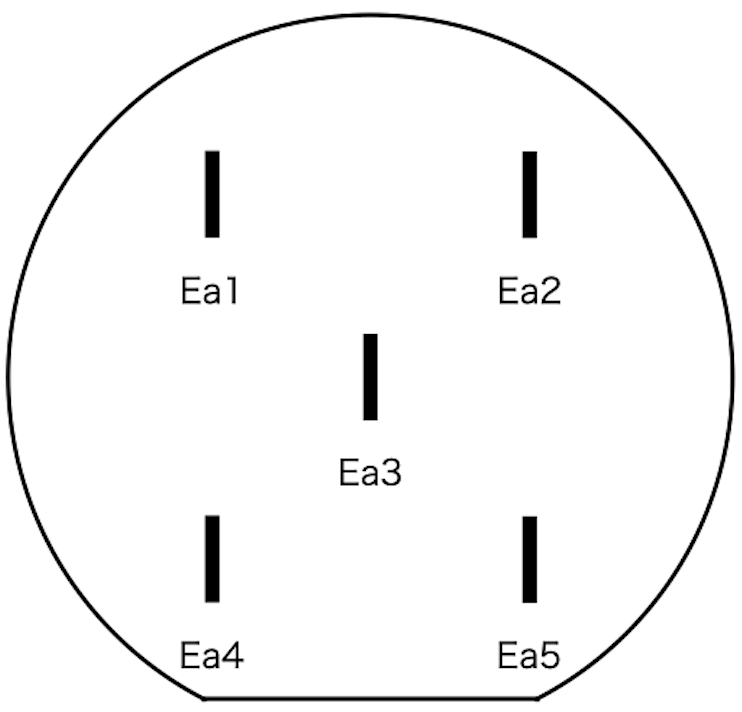
\includegraphics[width=0.5\textwidth]{BoardSchematic.png}
    \label{fig:BoardSchematic}
\end{figure}
\begin{figure}[H]
    \centering
    \begin{minipage}[t]{0.48\textwidth}
        \centering
        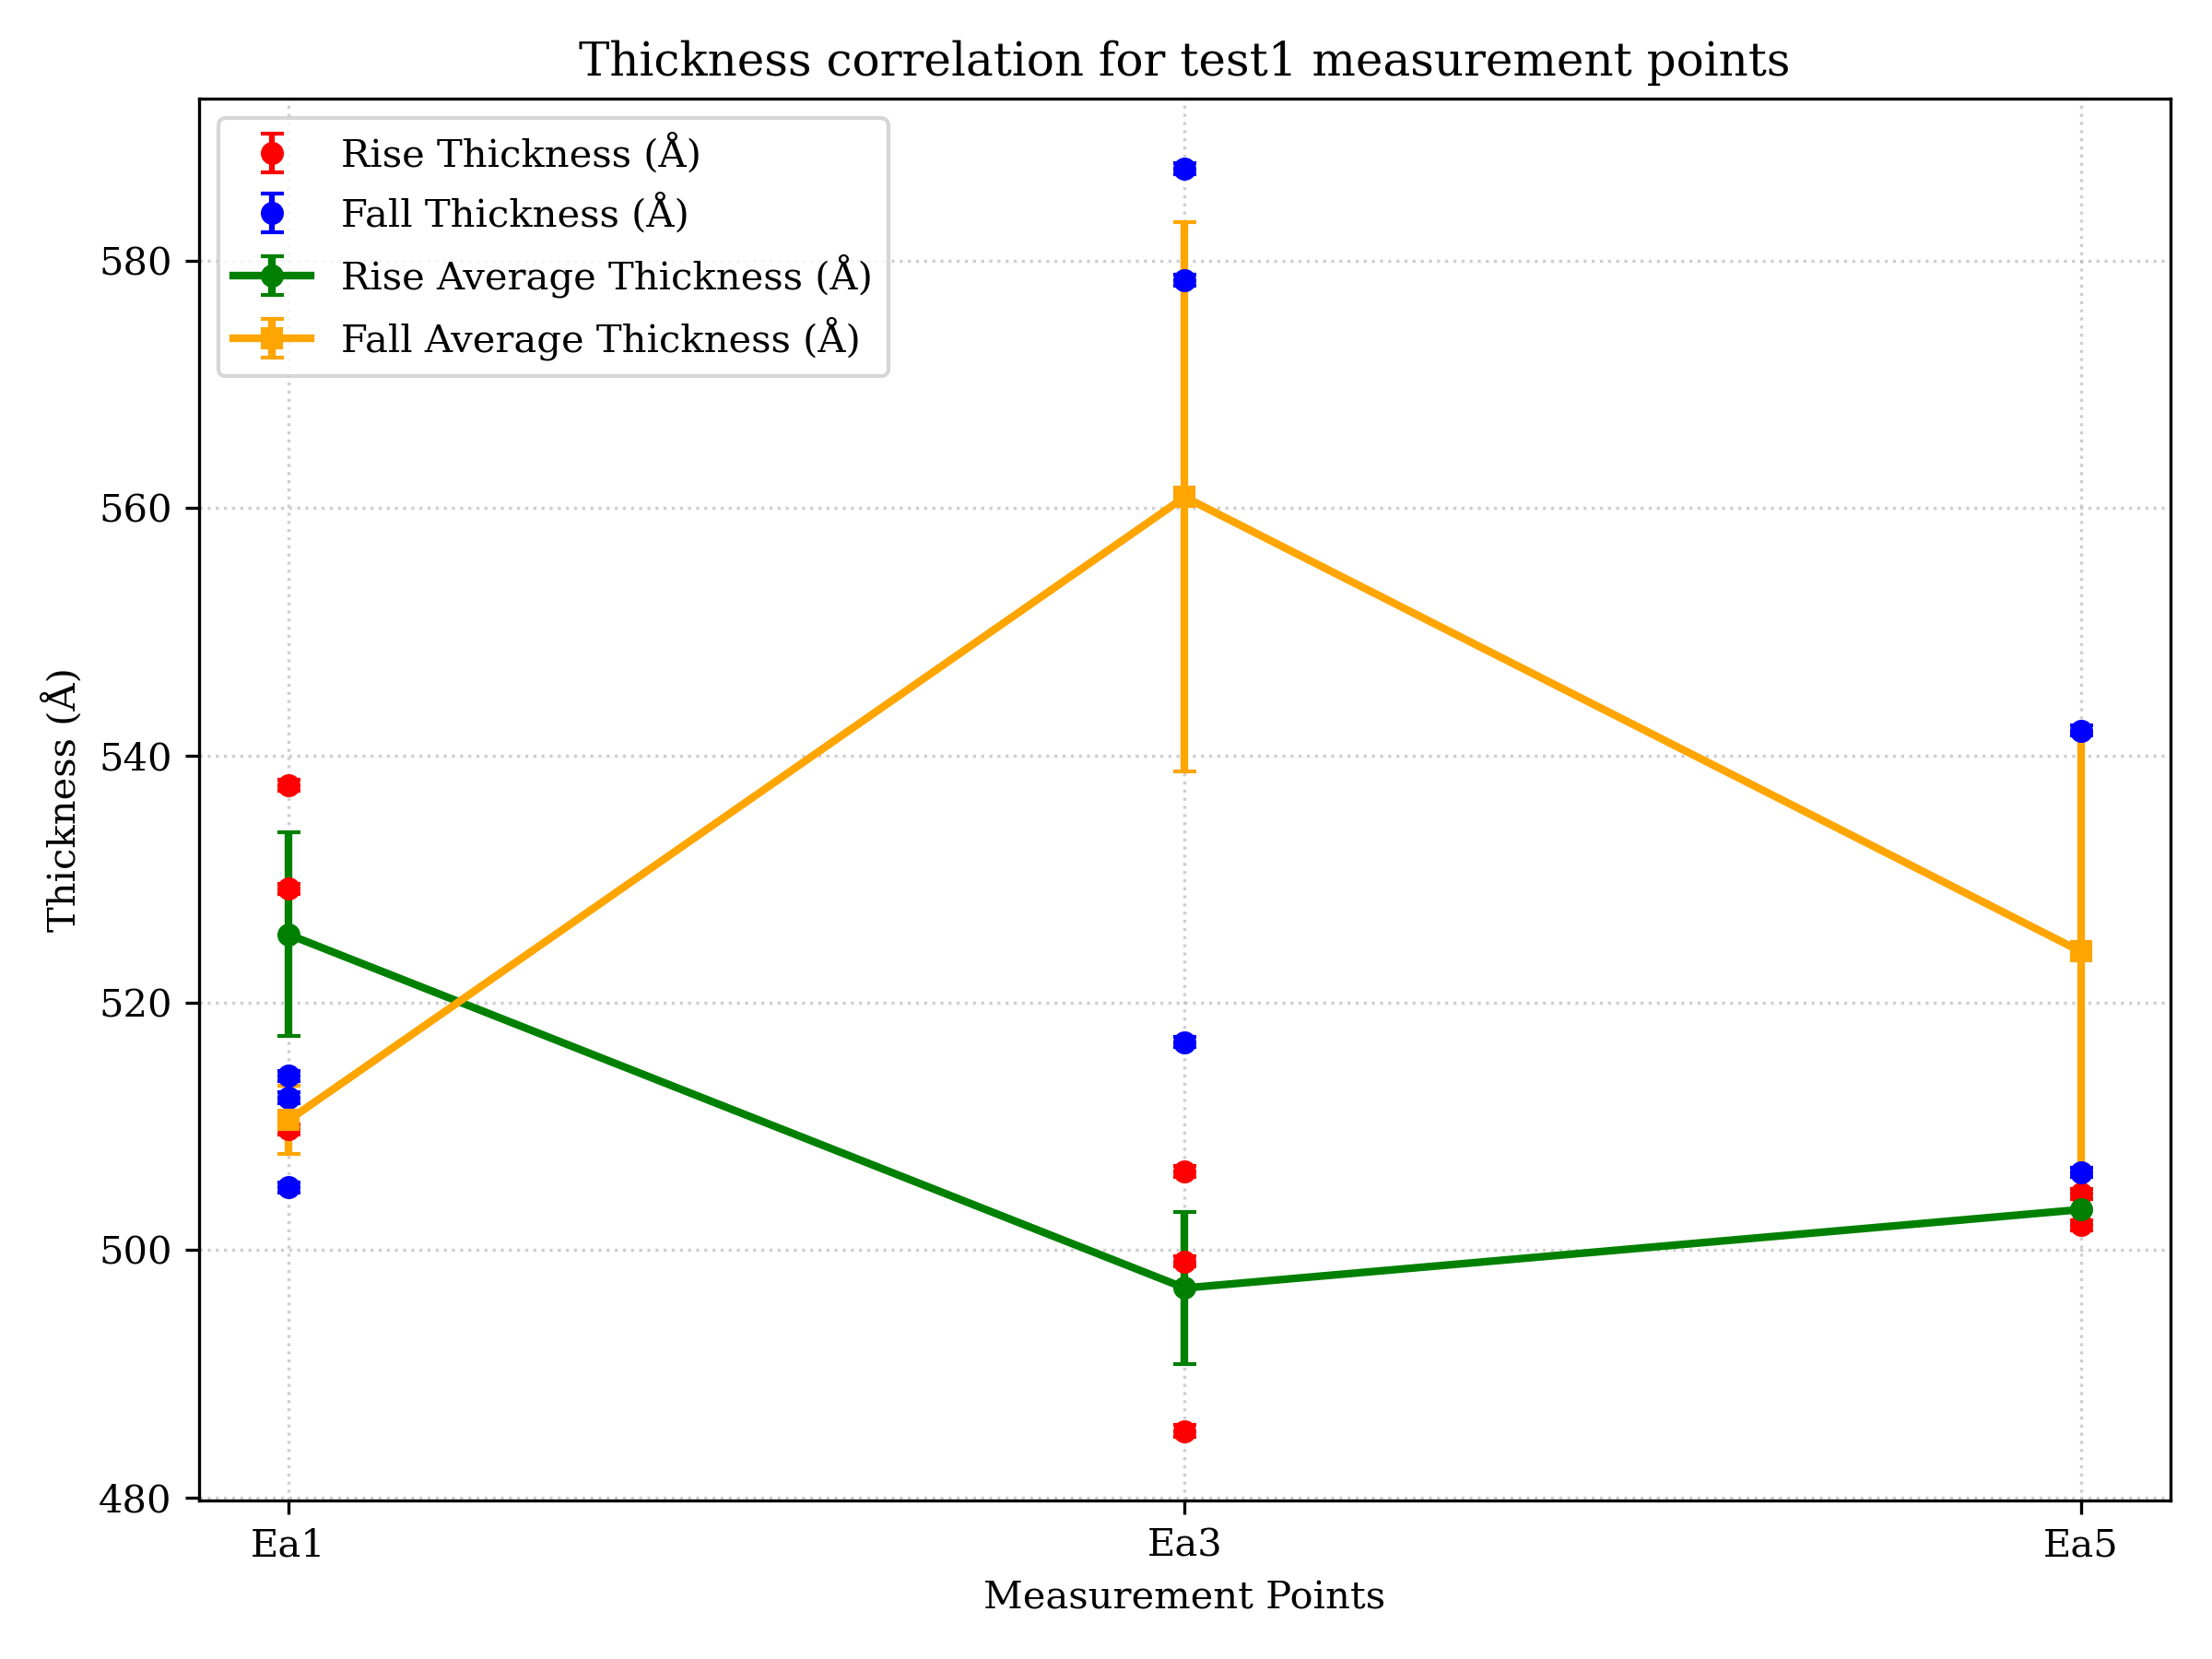
\includegraphics[width=\linewidth]{thickness_correlation_test1_Ea1-3-5.png}
    \end{minipage}
    \hfill
    \begin{minipage}[t]{0.48\textwidth}
        \centering
        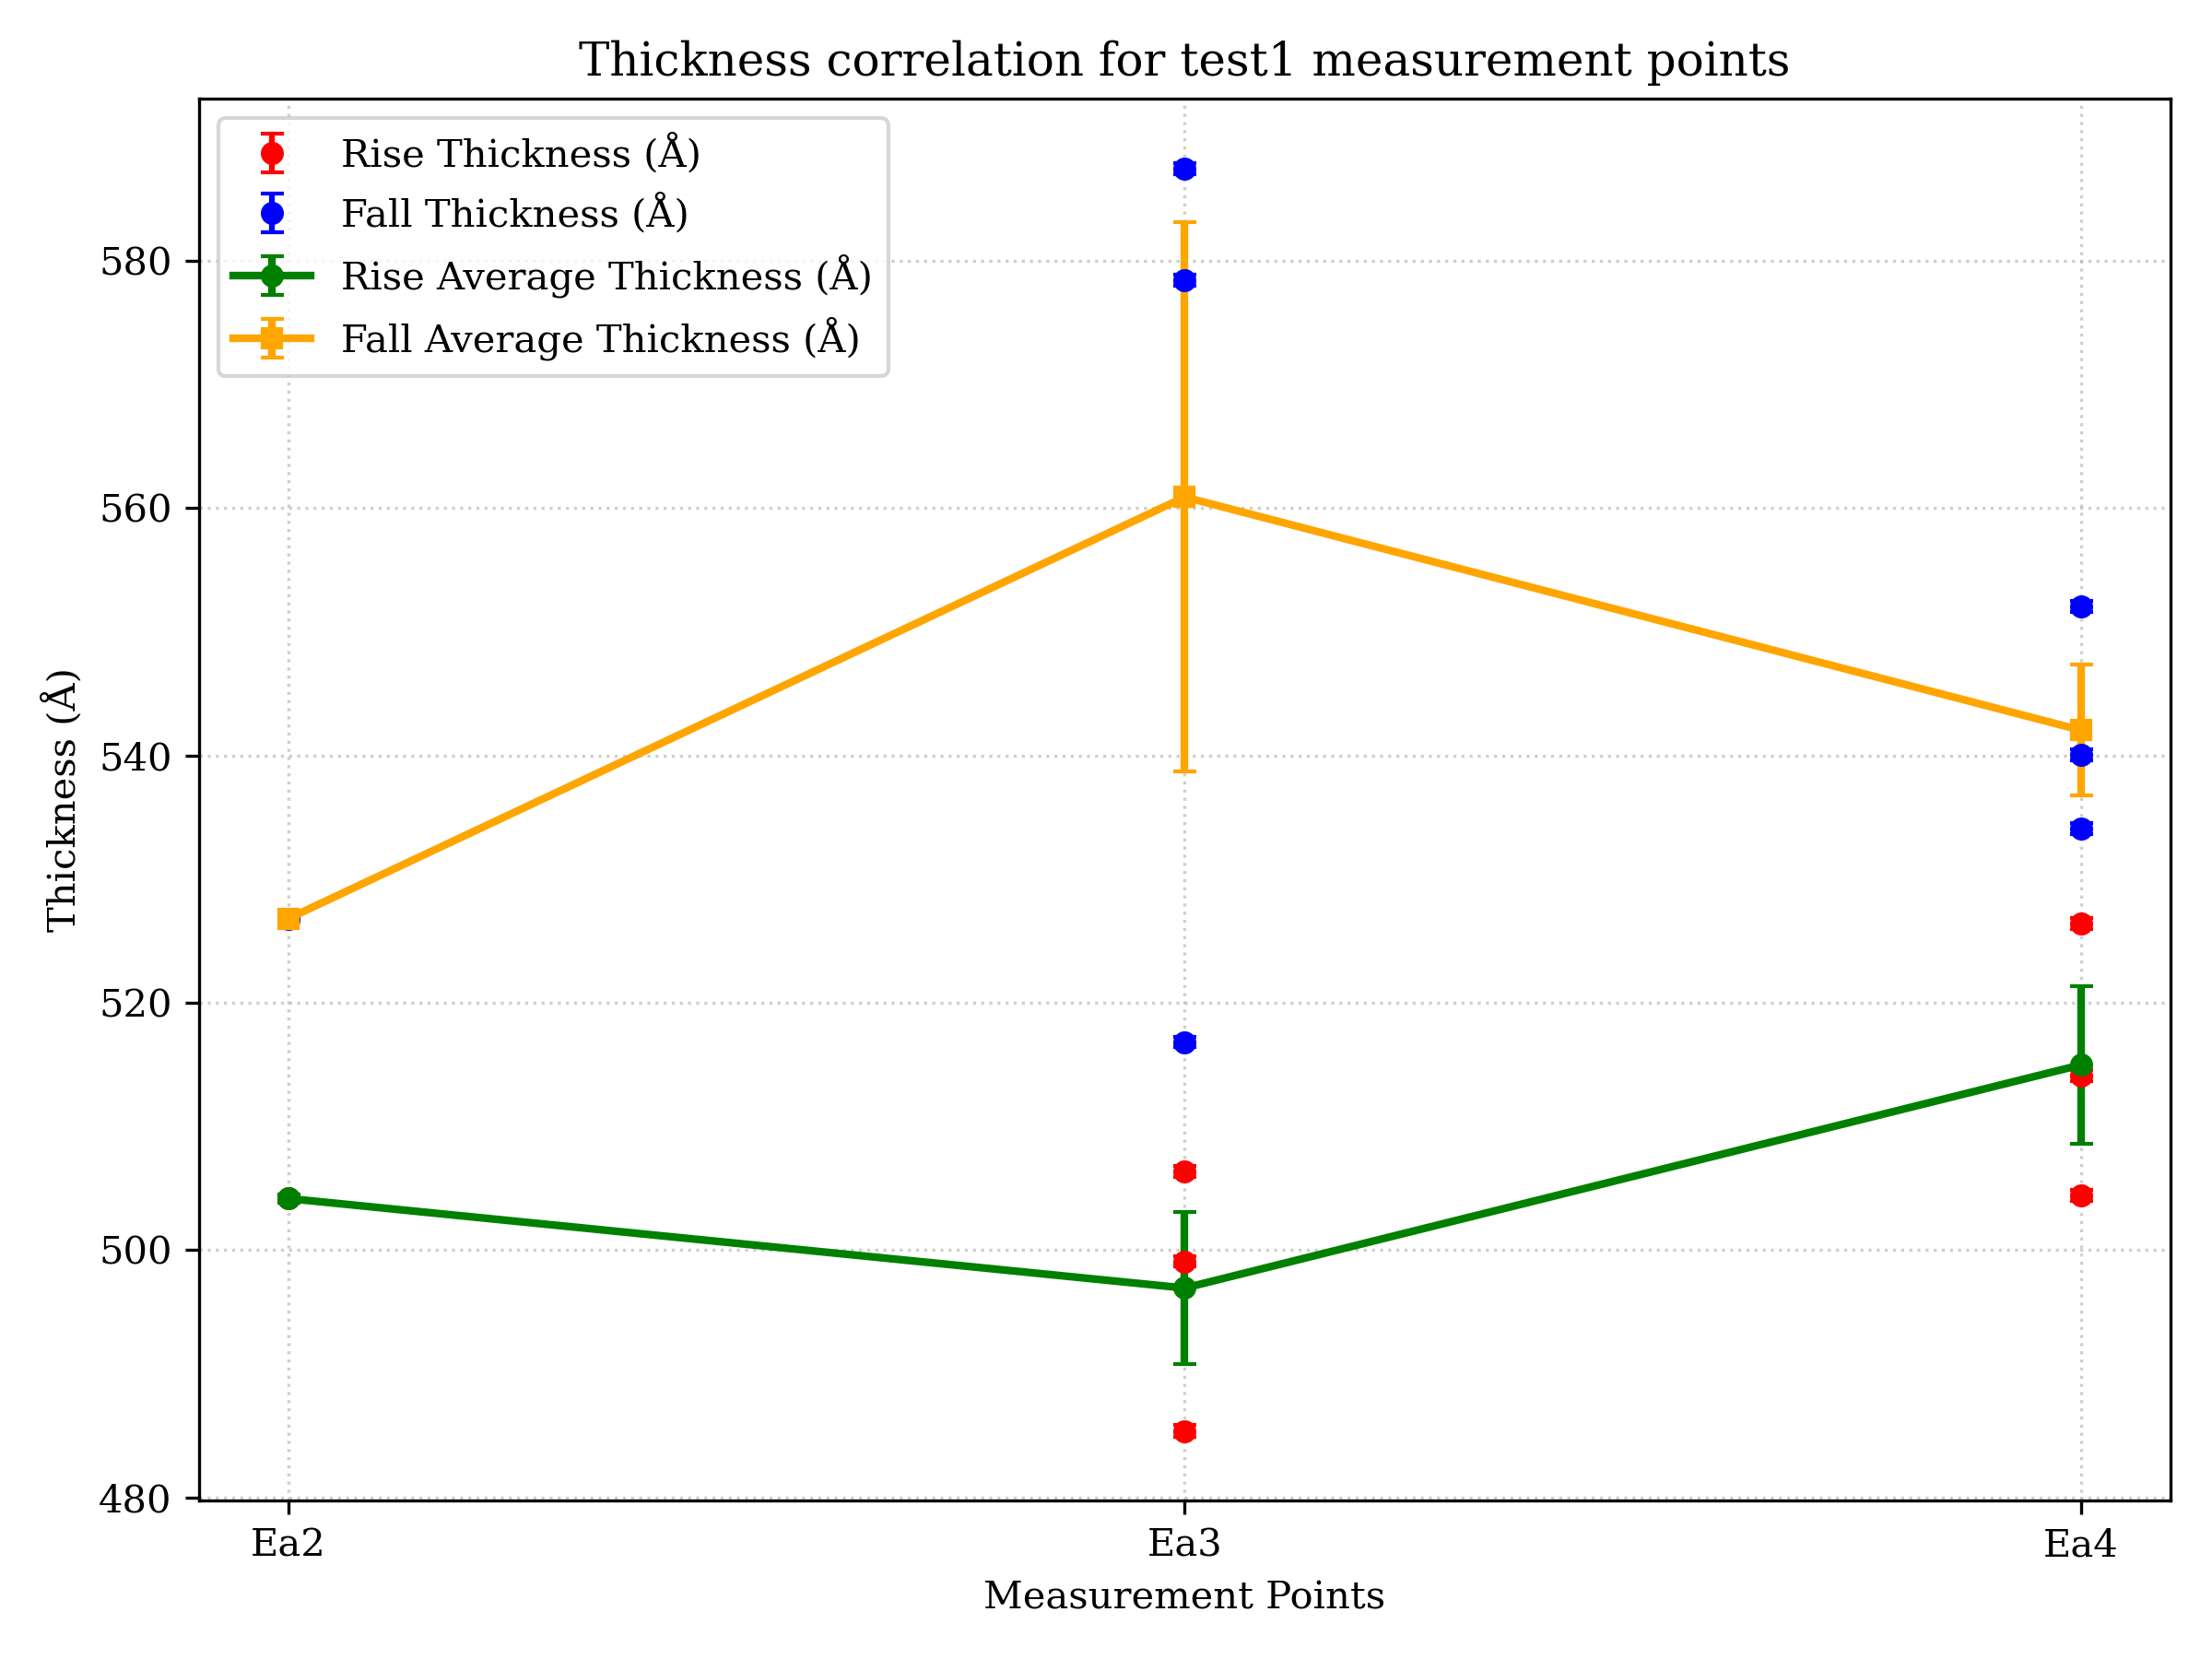
\includegraphics[width=\linewidth]{thickness_correlation_test1_Ea2-3-4.png}
    \end{minipage}
    \label{fig:test1_ea_correlations}
\end{figure}
\begin{figure}[H]
    \centering
    \begin{minipage}[t]{0.48\textwidth}
        \centering
        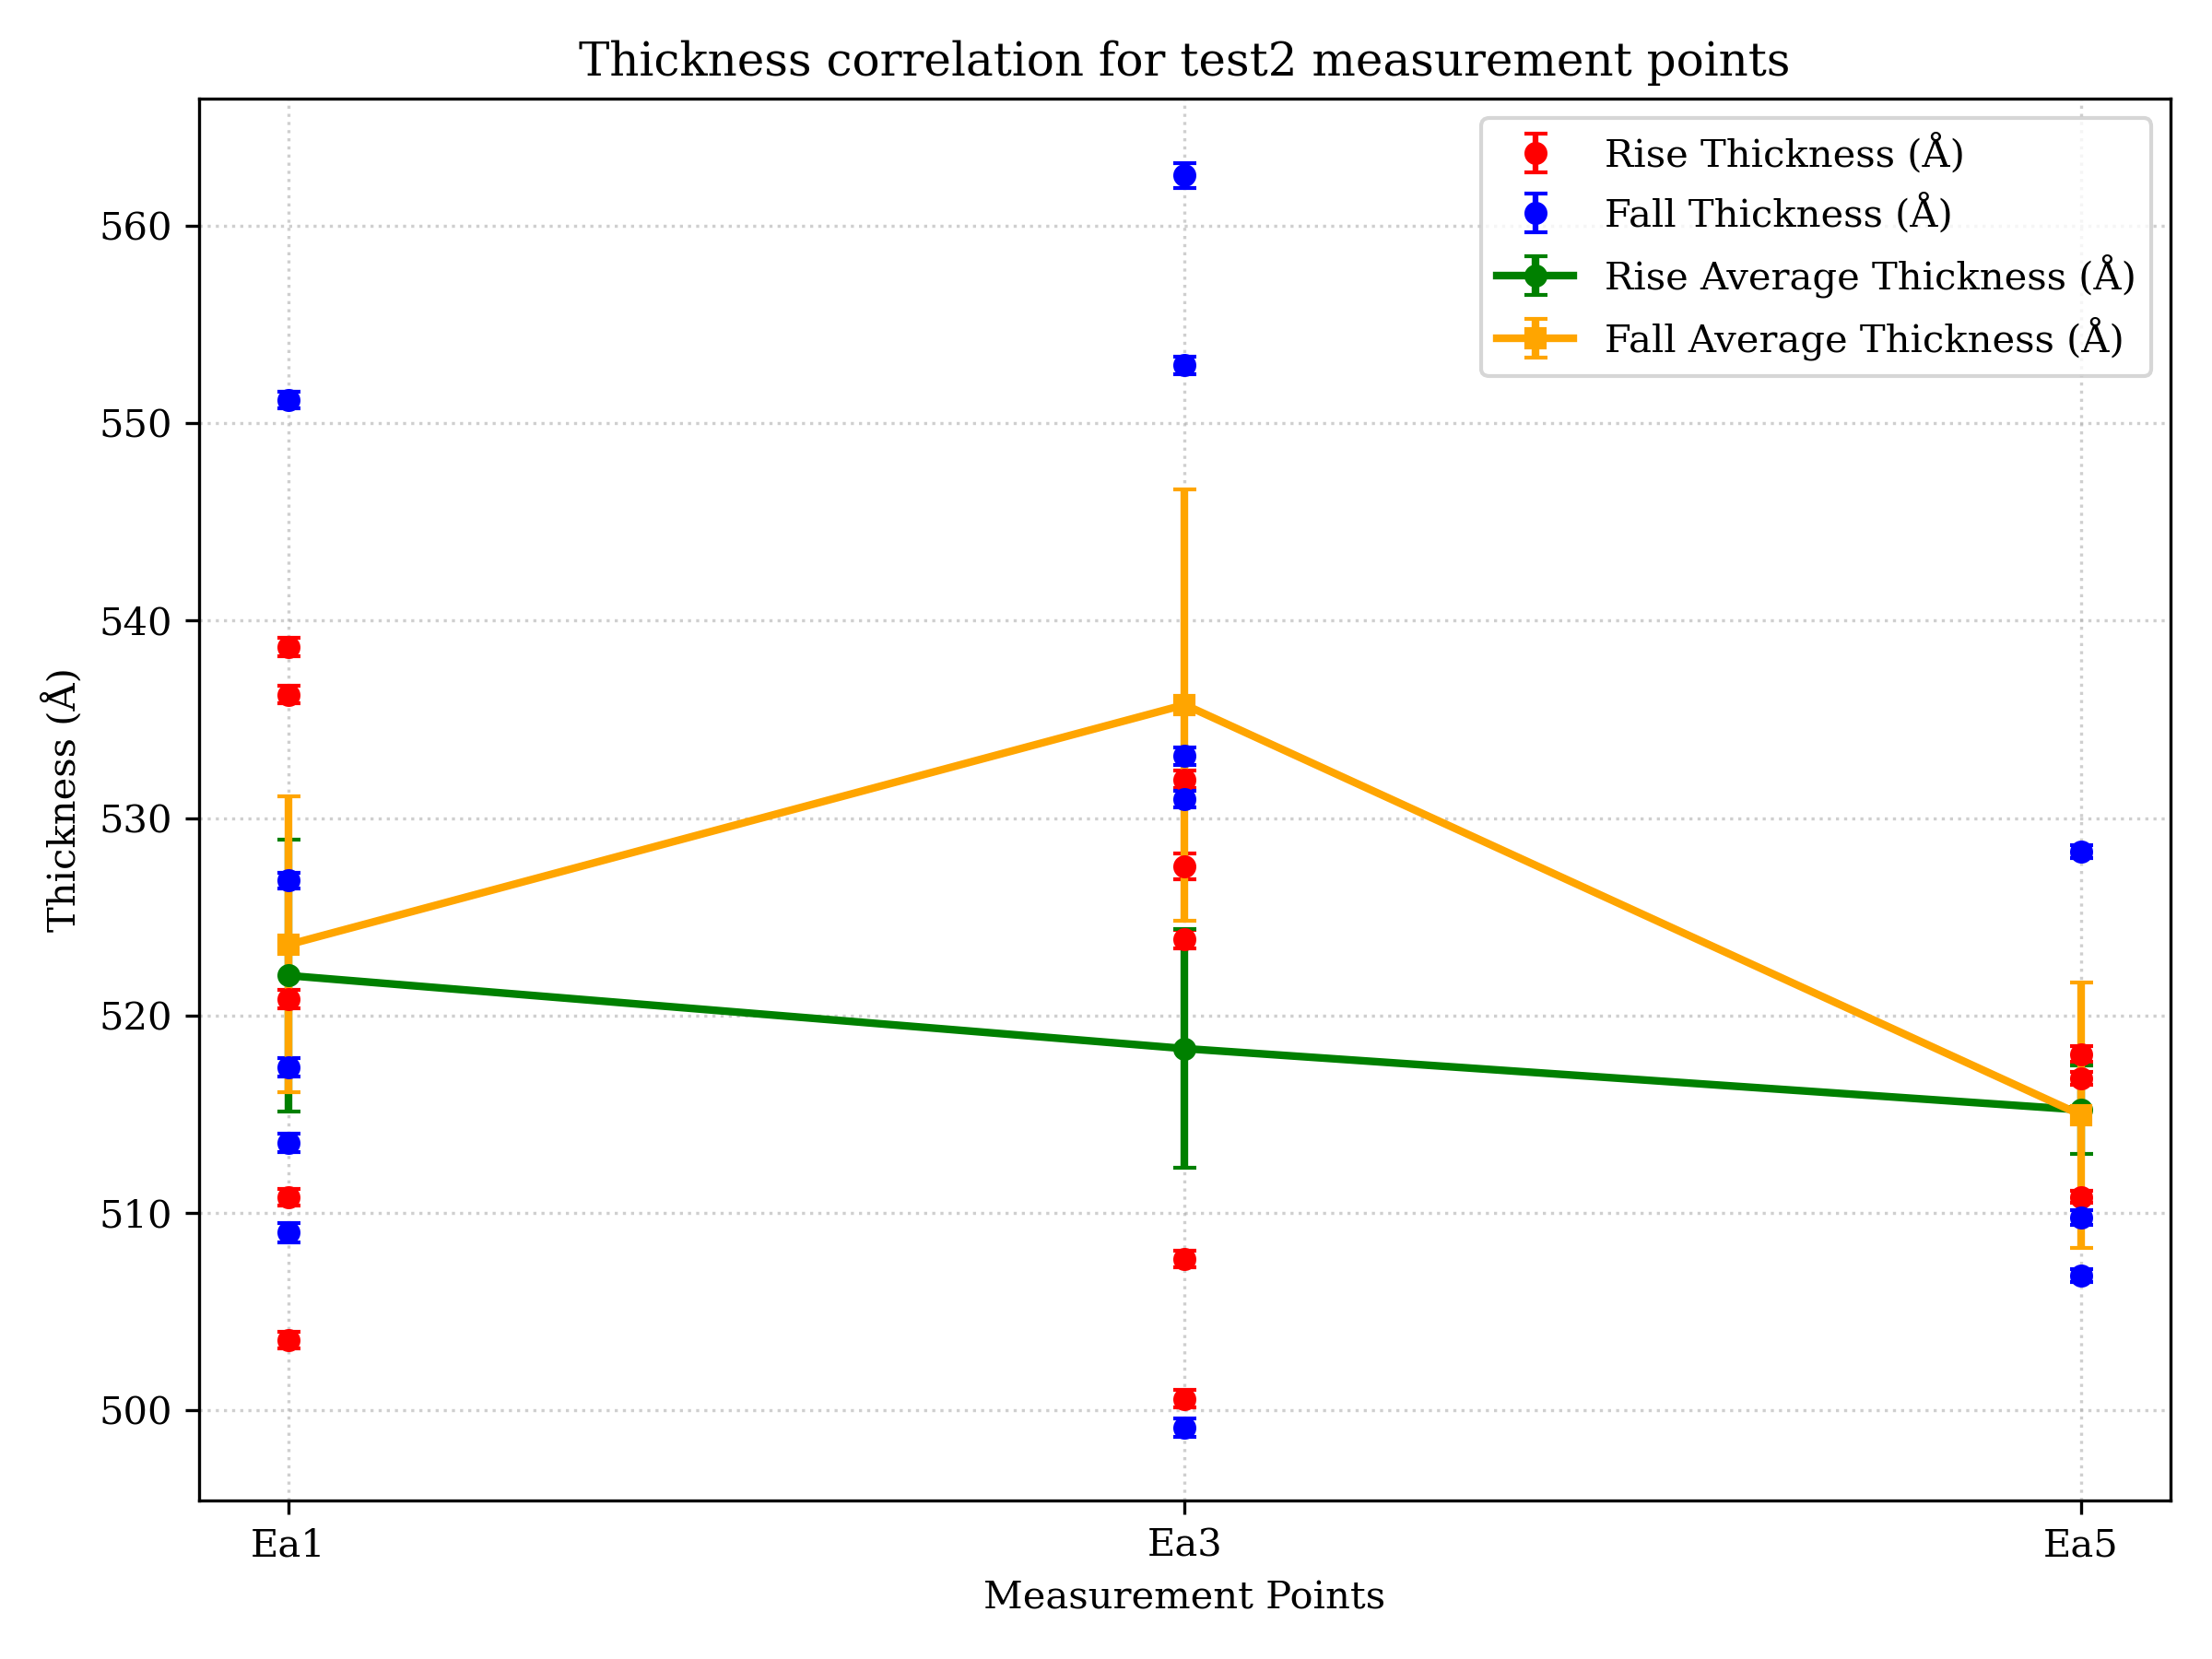
\includegraphics[width=\linewidth]{thickness_correlation_test2_Ea1-3-5.png}
    \end{minipage}
    \hfill
    \begin{minipage}[t]{0.48\textwidth}
        \centering
        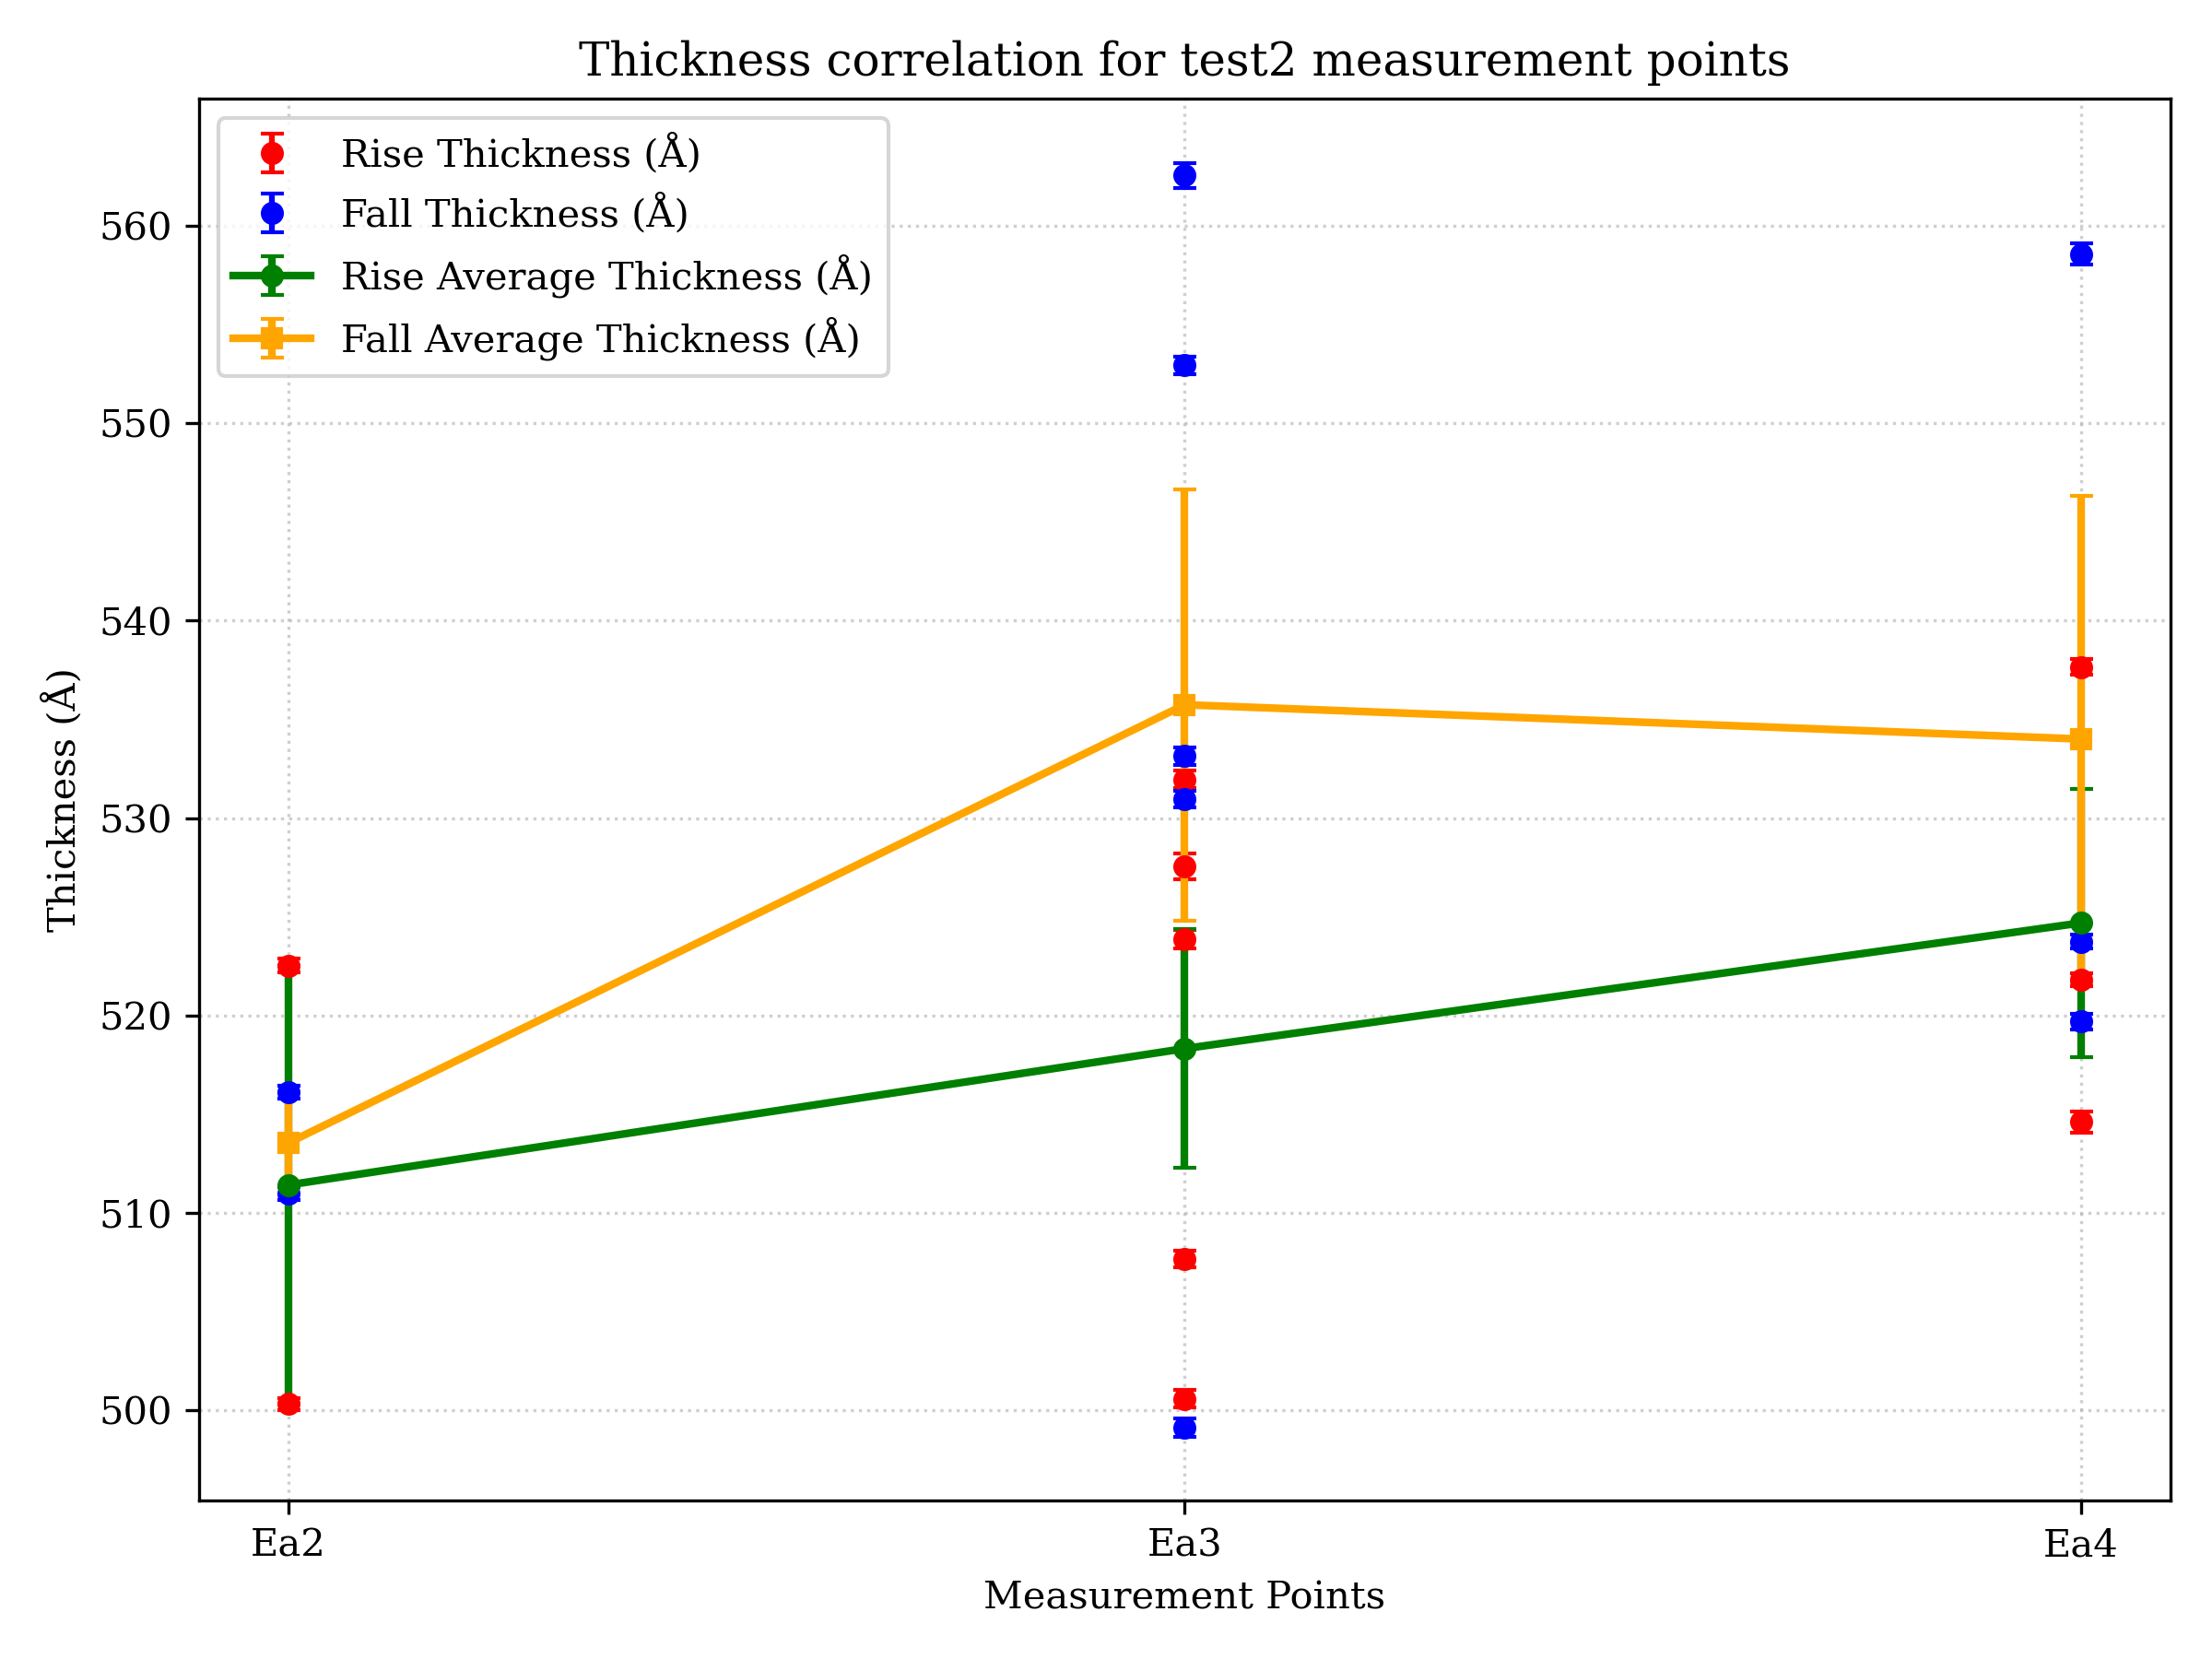
\includegraphics[width=\linewidth]{thickness_correlation_test2_Ea2-3-4.png}
    \end{minipage}
    \label{fig:test2_ea_correlations}
\end{figure}
\begin{figure}[H]
    \centering
    \begin{minipage}[t]{0.48\textwidth}
        \centering
        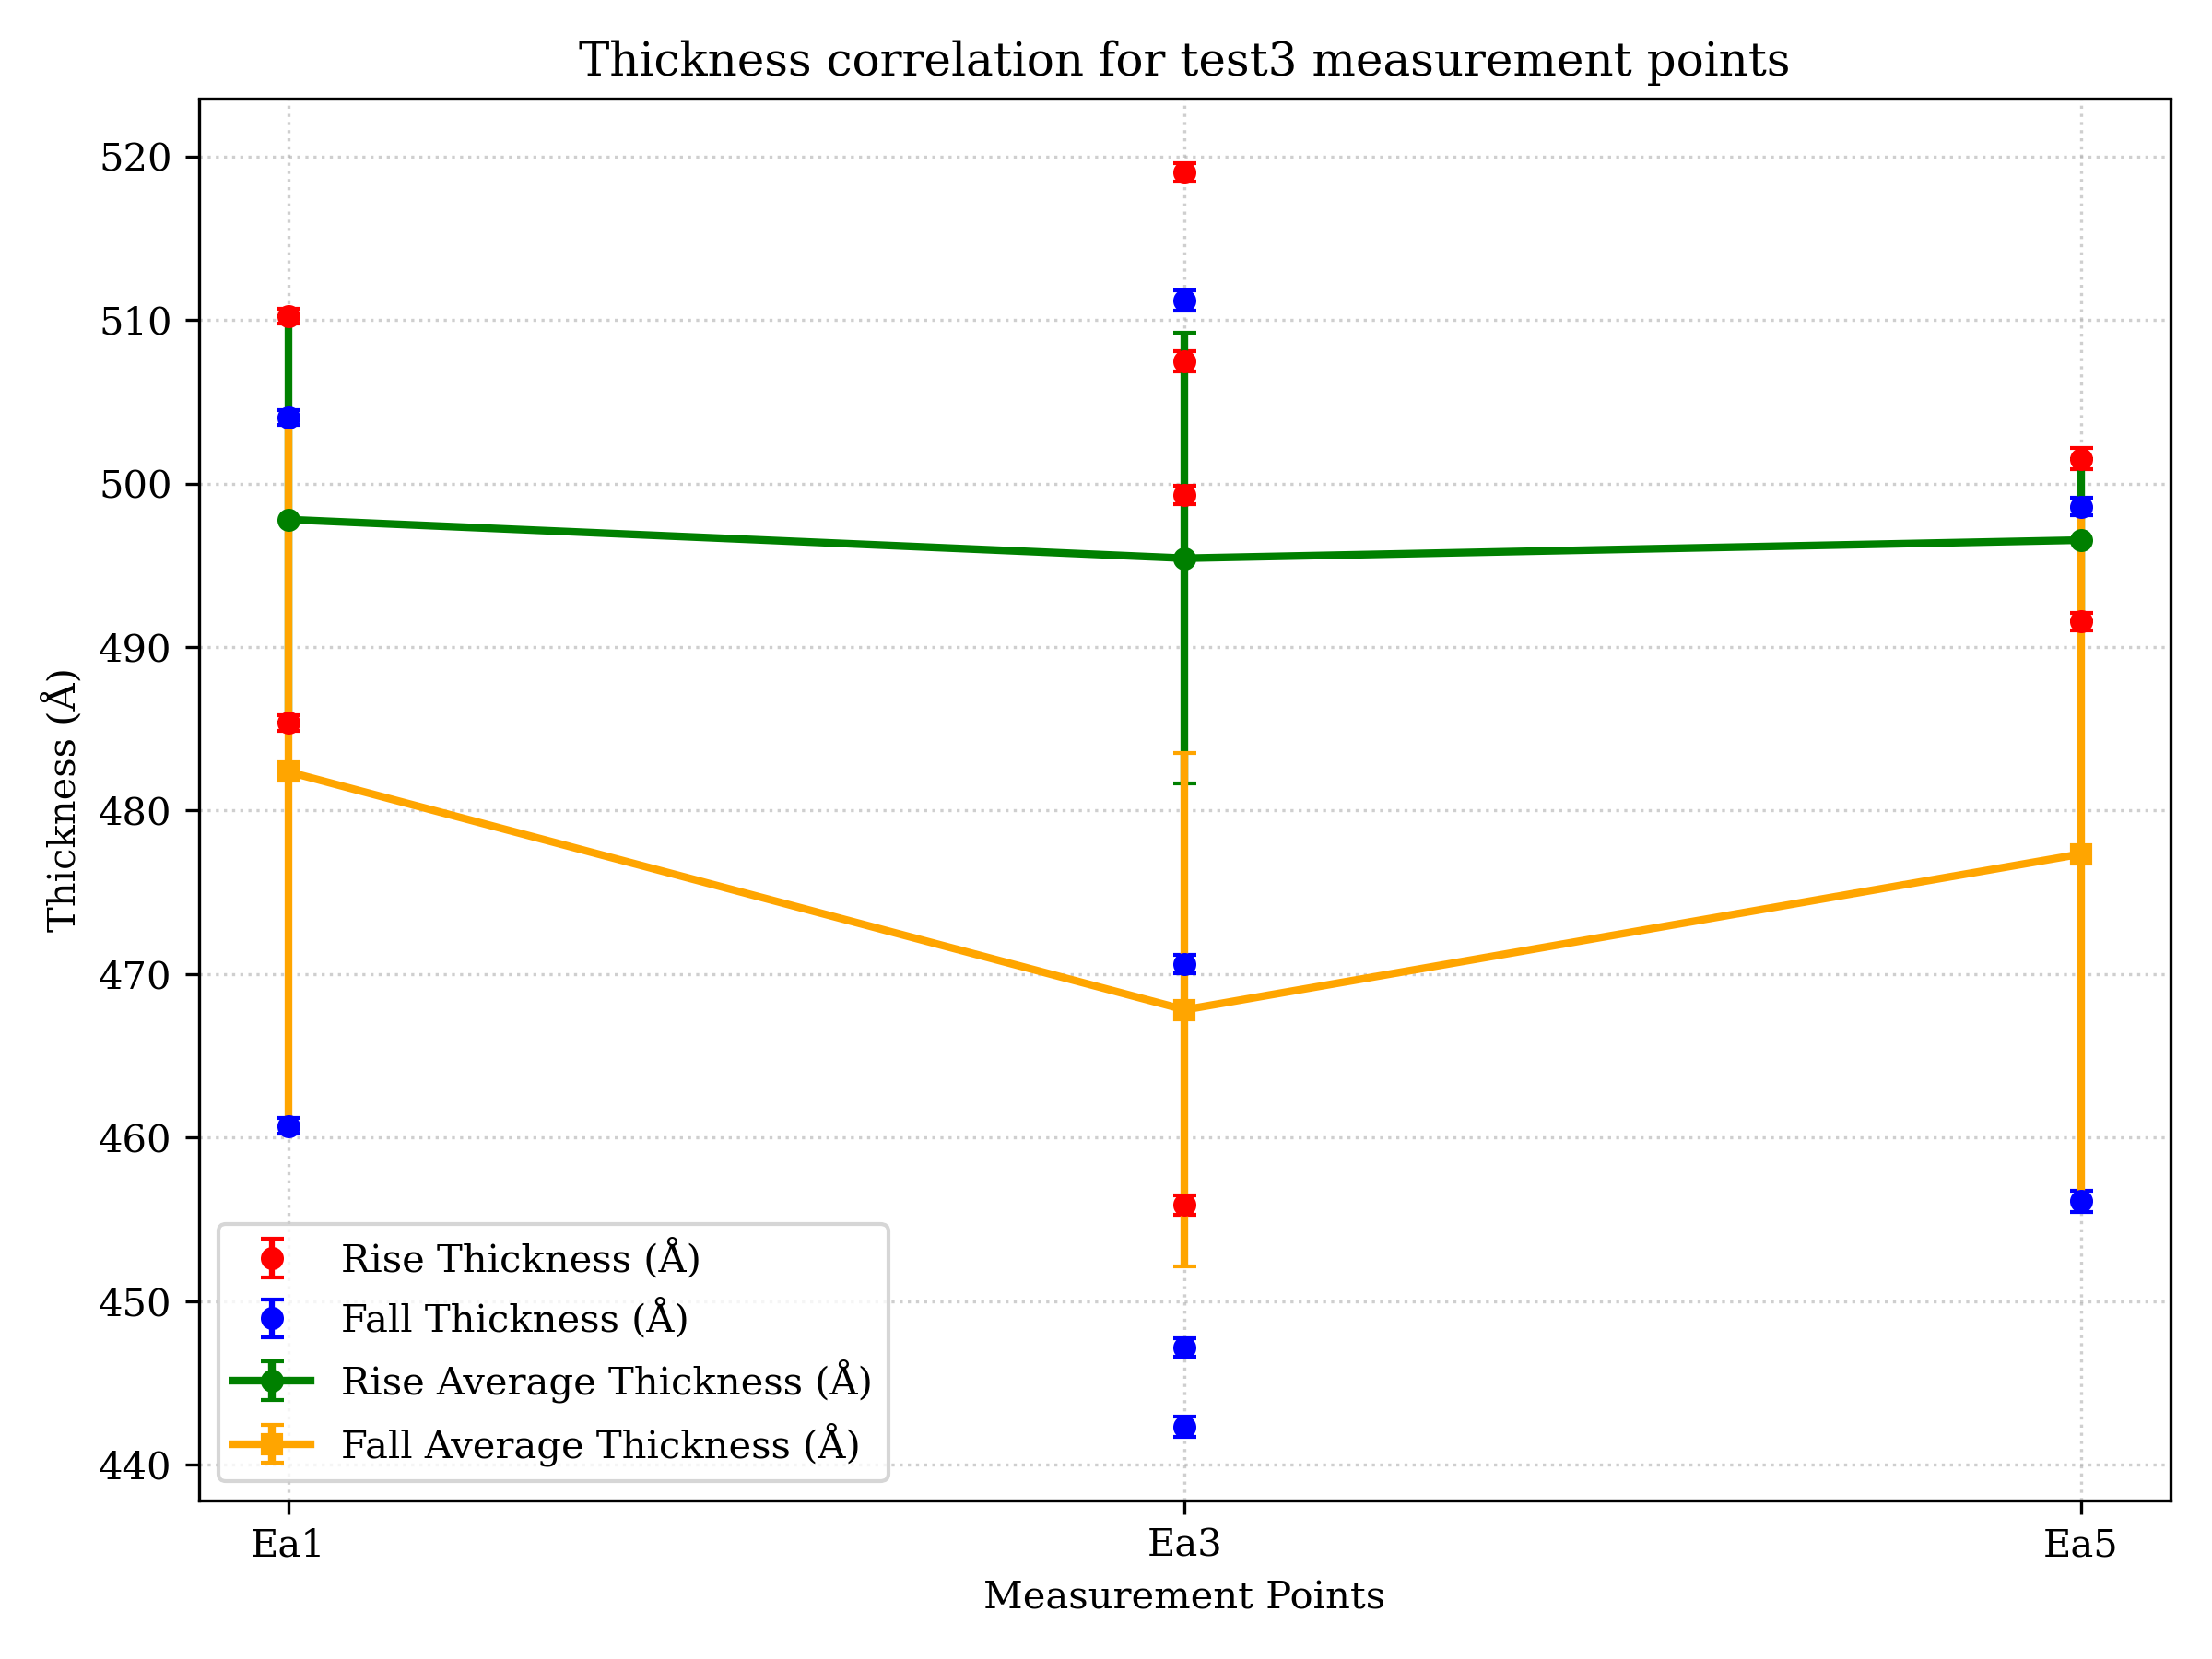
\includegraphics[width=\linewidth]{thickness_correlation_test3_Ea1-3-5.png}
    \end{minipage}
    \hfill
    \begin{minipage}[t]{0.48\textwidth}
        \centering
        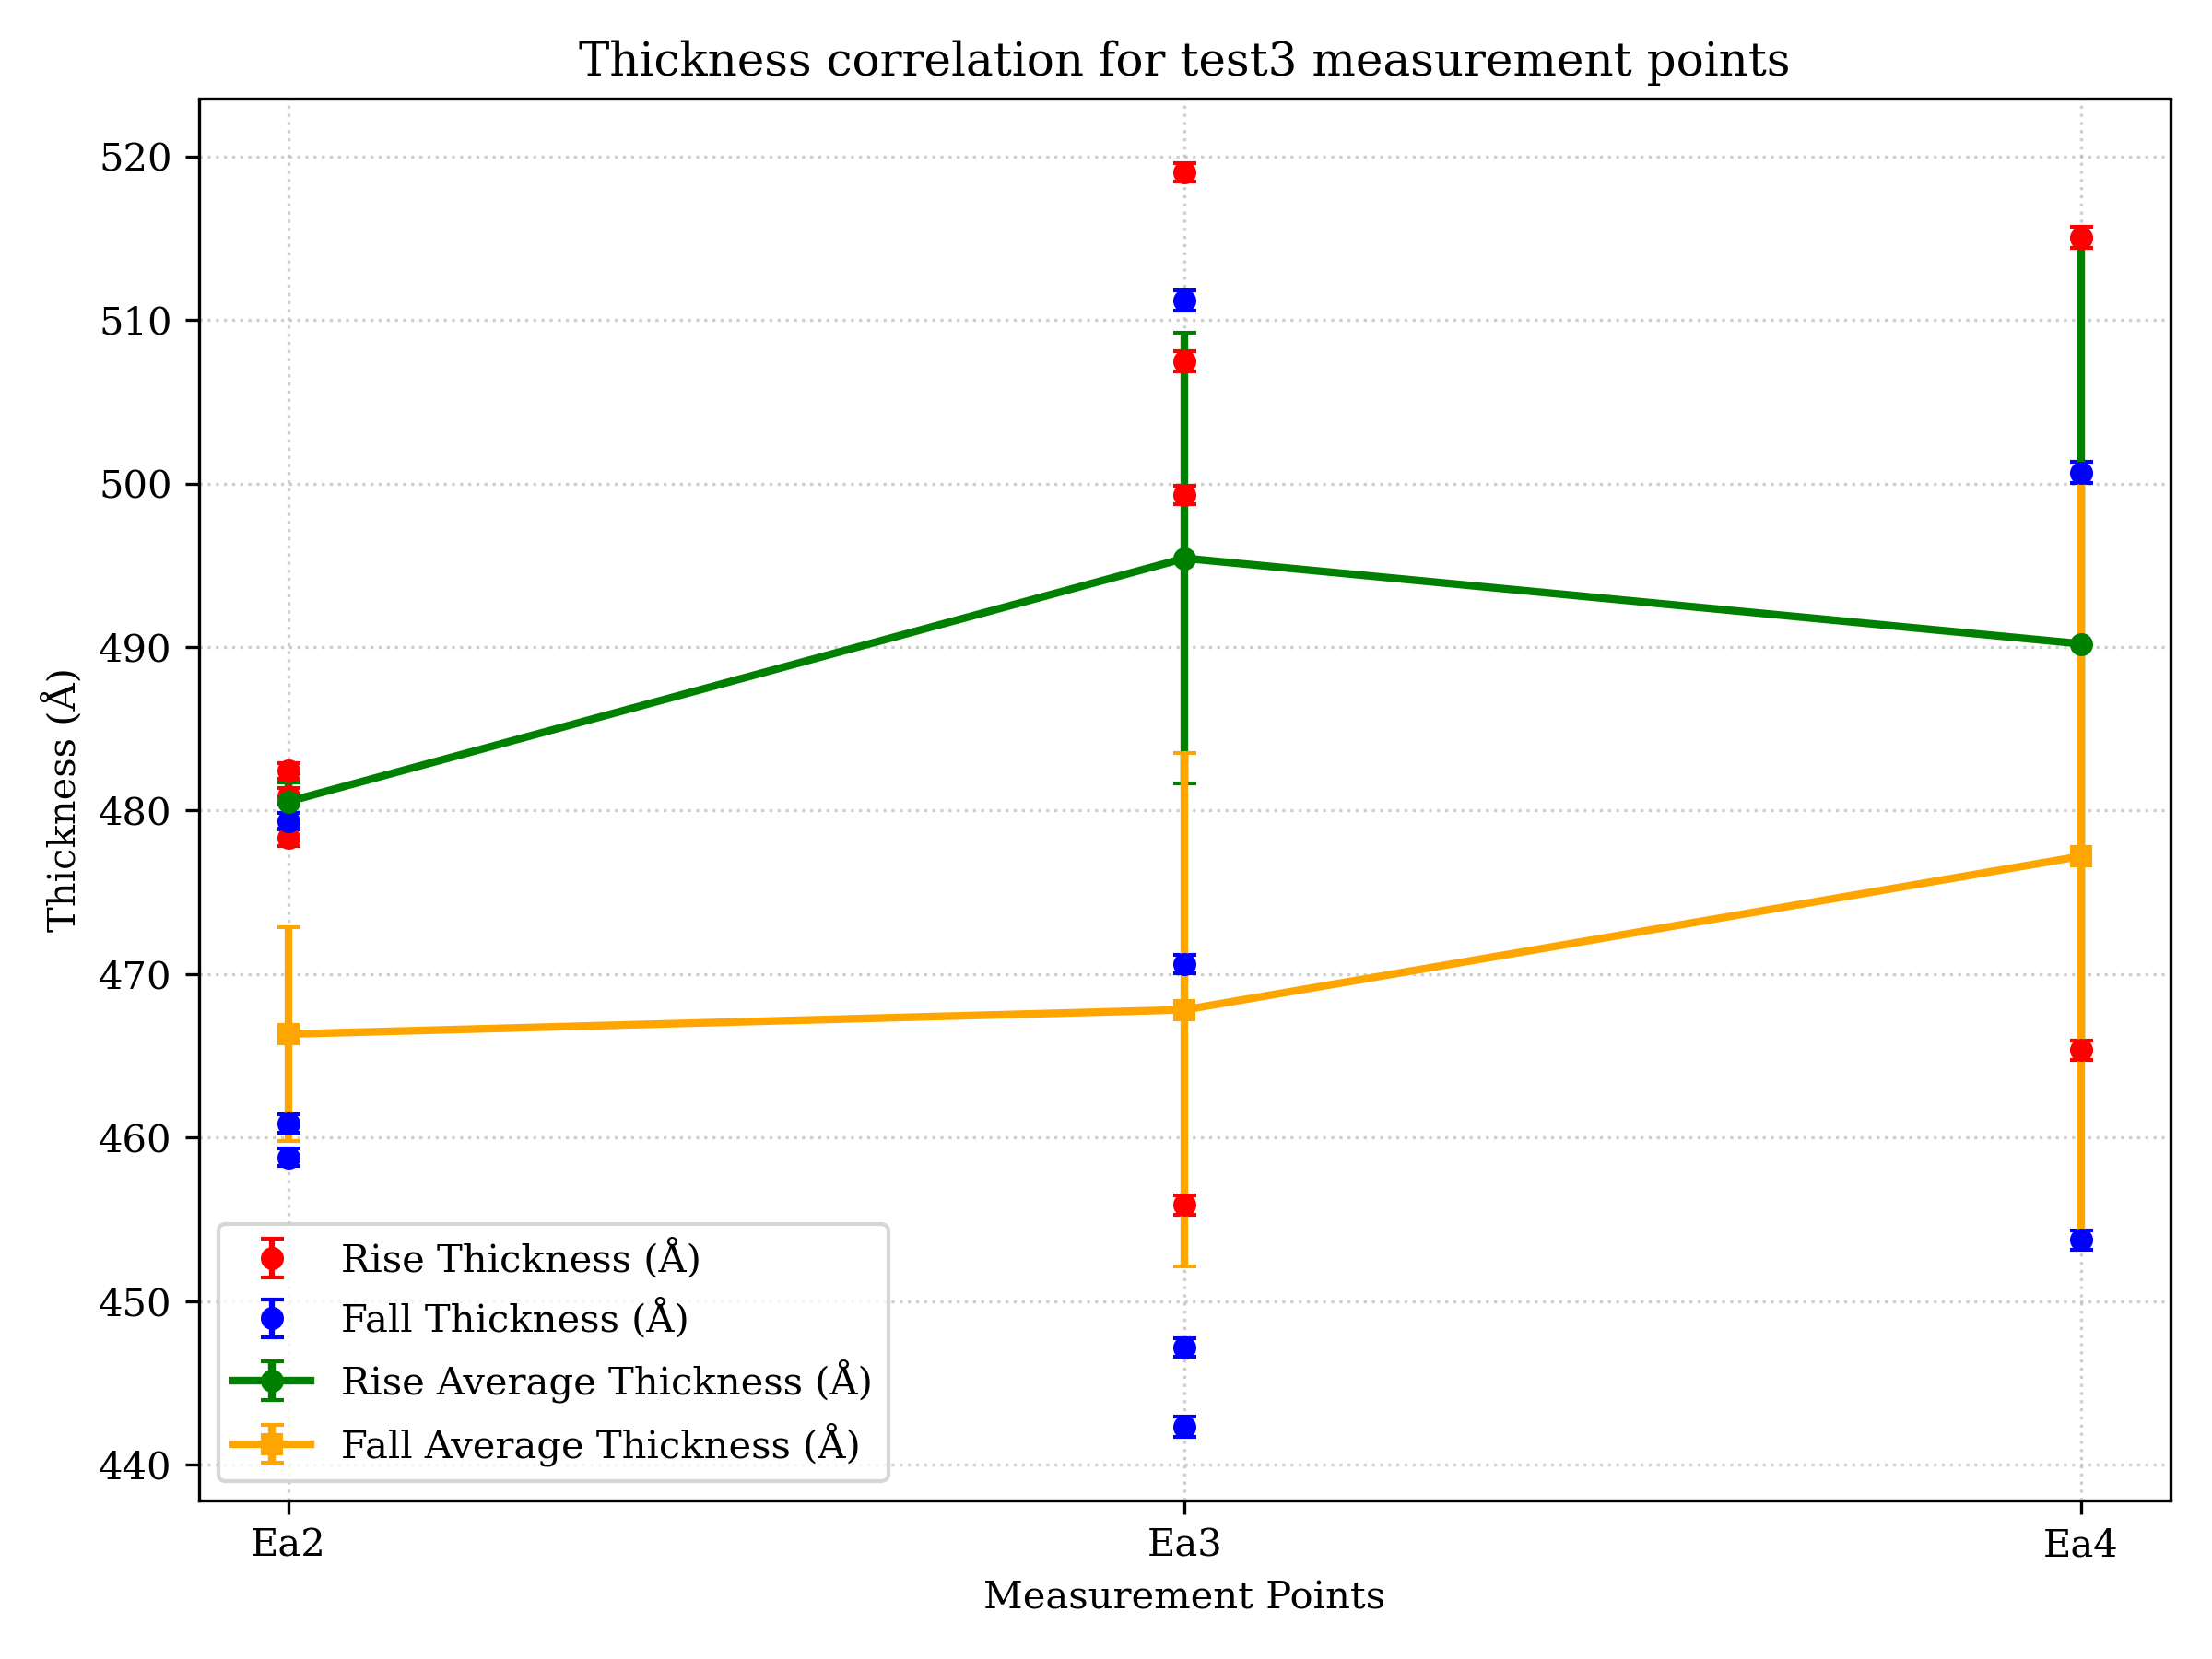
\includegraphics[width=\linewidth]{thickness_correlation_test3_Ea2-3-4.png}
    \end{minipage}
    \label{fig:test3_ea_correlations}
\end{figure}
\clearpage

\subsection*{Average Thickness Table}
各基板の位置ごとに,立ち上がり時間と立ち下がり時間による膜厚値の結果(平均値)を表にまとめる。
\par
誤差は,平均値の不偏標準偏差で計算する。
\begin{table}[H]
    \centering
    \begin{tabular}{ccD{+}{\,\pm\,}{6,6}D{+}{\,\pm\,}{6,6}D{+}{\,\pm\,}{6,6}D{+}{\,\pm\,}{6,6}D{+}{\,\pm\,}{6,6}}
        \toprule
        & & \multicolumn{1}{c}{Ea1} & \multicolumn{1}{c}{Ea2} & \multicolumn{1}{c}{Ea3} & \multicolumn{1}{c}{Ea4} & \multicolumn{1}{c}{Ea5} \\
        \midrule
        \multirow{2}{*}{test1} & Rise & 525.52+8.23 & 504.17+0.37 & 496.93+6.16 & 514.97+6.36 & 503.28+1.26 \\
        & Fall & 510.50+2.76 & 526.81+0.37 & 560.89+22.20 & 542.04+5.28 & 524.14+17.85 \\
        \addlinespace
        \multirow{2}{*}{test2} & Rise & 522.02+6.89 & 511.41+11.10 & 518.32+6.04 & 524.69+6.81 & 515.22+2.23 \\
        & Fall & 523.59+7.49 & 513.54+2.57 & 535.74+10.92 & 534.00+12.34 & 514.96+6.72 \\
        \addlinespace
        \multirow{2}{*}{test3} & Rise & 497.80+12.44 & 480.56+1.19 & 495.44+13.80 & 490.20+24.86 & 496.55+4.98 \\
        & Fall & 482.37+21.67 & 466.33+6.54 & 467.82+15.73 & 477.21+23.48 & 477.34+21.24 \\
        \bottomrule
    \end{tabular}
\end{table}
\clearpage

\section*{Thickness Results Table}
全測定データにおける膜厚値の表にまとめる。
\par
1列目から順に,データファイル名,立ち上がり始めの点,立ち上がり終わりの点,立ち上がりの膜厚値,立ち下がり始めの点,立ち下がり終わりの点,立ち下がりの膜厚値である。
\begin{table}[H]
    \resizebox{\textwidth}{!}{
        \begin{tabular}{lD{.}{.}{4.2}D{.}{.}{4.2}D{.}{.}{4.2}D{.}{.}{4.2}D{.}{.}{4.2}D{.}{.}{4.2}}
            \toprule
            \multicolumn{1}{c}{File Name} & \multicolumn{1}{c}{Pre-Rise Value ($\rm\AA$)} & \multicolumn{1}{c}{Post-Rise Value ($\rm\AA$)} & \multicolumn{1}{c}{Rise Height ($\rm\AA$)} & \multicolumn{1}{c}{Pre-Fall Value ($\rm\AA$)} & \multicolumn{1}{c}{Post-Fall Value ($\rm\AA$)} & \multicolumn{1}{c}{Fall Height ($\rm\AA$)} \\
            \midrule
            \hyperref[fig:LOR3Atest1250526LtoREa11]{LOR3A\_test1\_250526\_LtoR\_Ea1\_1.txt} & 1.23 & 510.99 & 509.77 & 805.17 & 300.09 & 505.08 \\
            \hyperref[fig:LOR3Atest1250526LtoREa31]{LOR3A\_test1\_250526\_LtoR\_Ea3\_1.txt} & 20.86 & 527.23 & 506.37 & 1060.57 & 482.16 & 578.42 \\
            \hyperref[fig:LOR3Atest1250526LtoREa32]{LOR3A\_test1\_250526\_LtoR\_Ea3\_2.txt} & 30.36 & 529.43 & 499.07 & 809.80 & 292.99 & 516.80 \\
            \hyperref[fig:LOR3Atest1250526LtoREa41]{LOR3A\_test1\_250526\_LtoR\_Ea4\_1.txt} & 11.35 & 537.74 & 526.39 & 967.17 & 427.15 & 540.02 \\
            \hyperref[fig:LOR3Atest1250526LtoREa51]{LOR3A\_test1\_250526\_LtoR\_Ea5\_1.txt} & -54.46 & 450.08 & 504.54 & 640.59 & 98.60 & 541.99 \\
            \hyperref[fig:LOR3Atest1250526RtoLEa11]{LOR3A\_test1\_250526\_RtoL\_Ea1\_1.txt} & -8.11 & 521.10 & 529.21 & 515.50 & 1.42 & 514.08 \\
            \hyperref[fig:LOR3Atest1250526RtoLEa12]{LOR3A\_test1\_250526\_RtoL\_Ea1\_2.txt} & 5.40 & 542.96 & 537.56 & 745.09 & 232.75 & 512.34 \\
            \hyperref[fig:LOR3Atest1250526RtoLEa21]{LOR3A\_test1\_250526\_RtoL\_Ea2\_1.txt} & -4.71 & 499.46 & 504.17 & 838.00 & 311.19 & 526.81 \\
            \hyperref[fig:LOR3Atest1250526RtoLEa31]{LOR3A\_test1\_250526\_RtoL\_Ea3\_1.txt} & 13.87 & 499.24 & 485.37 & 845.68 & 258.24 & 587.44 \\
            \hyperref[fig:LOR3Atest1250526RtoLEa41]{LOR3A\_test1\_250526\_RtoL\_Ea4\_1.txt} & -9.05 & 505.07 & 514.12 & 766.10 & 214.09 & 552.01 \\
            \hyperref[fig:LOR3Atest1250526RtoLEa42]{LOR3A\_test1\_250526\_RtoL\_Ea4\_2.txt} & -7.97 & 496.44 & 504.41 & 739.43 & 205.36 & 534.07 \\
            \hyperref[fig:LOR3Atest1250526RtoLEa51]{LOR3A\_test1\_250526\_RtoL\_Ea5\_1.txt} & -26.66 & 475.36 & 502.02 & 783.02 & 276.73 & 506.29 \\
            \hyperref[fig:LOR3Atest1250526test]{LOR3A\_test1\_250526\_test.txt} & 36.25 & 533.44 & 497.19 & 524.52 & 48.71 & 475.80 \\
            \hyperref[fig:LOR3Atest2250526LtoREa11]{LOR3A\_test2\_250526\_LtoR\_Ea1\_1.txt} & 8.32 & 547.00 & 538.67 & 638.16 & 124.61 & 513.55 \\
            \hyperref[fig:LOR3Atest2250526LtoREa12]{LOR3A\_test2\_250526\_LtoR\_Ea1\_2.txt} & -4.41 & 499.14 & 503.56 & 504.44 & -22.39 & 526.83 \\
            \hyperref[fig:LOR3Atest2250526LtoREa21]{LOR3A\_test2\_250526\_LtoR\_Ea2\_1.txt} & 20.21 & 520.52 & 500.31 & 519.61 & 3.49 & 516.11 \\
            \hyperref[fig:LOR3Atest2250526LtoREa31]{LOR3A\_test2\_250526\_LtoR\_Ea3\_1.txt} & 5.86 & 533.41 & 527.55 & 545.71 & -16.85 & 562.56 \\
            \hyperref[fig:LOR3Atest2250526LtoREa32]{LOR3A\_test2\_250526\_LtoR\_Ea3\_2.txt} & 10.40 & 510.98 & 500.58 & 528.07 & -2.88 & 530.95 \\
            \hyperref[fig:LOR3Atest2250526LtoREa33]{LOR3A\_test2\_250526\_LtoR\_Ea3\_3.txt} & 17.73 & 525.38 & 507.65 & 534.04 & 0.91 & 533.13 \\
            \hyperref[fig:LOR3Atest2250526LtoREa41]{LOR3A\_test2\_250526\_LtoR\_Ea4\_1.txt} & -2.94 & 511.66 & 514.60 & 619.40 & 60.83 & 558.57 \\
            \hyperref[fig:LOR3Atest2250526LtoREa42]{LOR3A\_test2\_250526\_LtoR\_Ea4\_2.txt} & -24.05 & 513.60 & 537.65 & 521.78 & 2.08 & 519.70 \\
            \hyperref[fig:LOR3Atest2250526LtoREa51]{LOR3A\_test2\_250526\_LtoR\_Ea5\_1.txt} & -25.36 & 492.68 & 518.03 & 498.48 & -11.28 & 509.76 \\
            \hyperref[fig:LOR3Atest2250526LtoREa52]{LOR3A\_test2\_250526\_LtoR\_Ea5\_2.txt} & 11.75 & 522.56 & 510.81 & 501.51 & -5.32 & 506.83 \\
            \hyperref[fig:LOR3Atest2250526RtoLEa11]{LOR3A\_test2\_250526\_RtoL\_Ea1\_1.txt} & -13.66 & 497.13 & 510.79 & 562.00 & 10.83 & 551.17 \\
            \hyperref[fig:LOR3Atest2250526RtoLEa12]{LOR3A\_test2\_250526\_RtoL\_Ea1\_2.txt} & -2.47 & 518.36 & 520.82 & 536.04 & 27.04 & 509.00 \\
            \hyperref[fig:LOR3Atest2250526RtoLEa13]{LOR3A\_test2\_250526\_RtoL\_Ea1\_3.txt} & -12.38 & 523.88 & 536.25 & 553.72 & 36.34 & 517.38 \\
            \hyperref[fig:LOR3Atest2250526RtoLEa21]{LOR3A\_test2\_250526\_RtoL\_Ea2\_1.txt} & 18.24 & 540.76 & 522.51 & 532.89 & 21.92 & 510.98 \\
            \hyperref[fig:LOR3Atest2250526RtoLEa31]{LOR3A\_test2\_250526\_RtoL\_Ea3\_1.txt} & -21.99 & 509.97 & 531.96 & 703.12 & 150.18 & 552.94 \\
            \hyperref[fig:LOR3Atest2250526RtoLEa32]{LOR3A\_test2\_250526\_RtoL\_Ea3\_2.txt} & 17.78 & 541.63 & 523.85 & 511.61 & 12.49 & 499.12 \\
            \hyperref[fig:LOR3Atest2250526RtoLEa41]{LOR3A\_test2\_250526\_RtoL\_Ea4\_1.txt} & 10.95 & 532.76 & 521.81 & 523.16 & -0.58 & 523.74 \\
            \hyperref[fig:LOR3Atest2250526RtoLEa51]{LOR3A\_test2\_250526\_RtoL\_Ea5\_1.txt} & -11.97 & 504.84 & 516.80 & 506.98 & -21.31 & 528.29 \\
            \hyperref[fig:LOR3Atest3250526LtoREa11]{LOR3A\_test3\_250526\_LtoR\_Ea1\_1.txt} & -1.55 & 483.81 & 485.36 & 507.71 & 47.01 & 460.70 \\
            \hyperref[fig:LOR3Atest3250526LtoREa21]{LOR3A\_test3\_250526\_LtoR\_Ea2\_1.txt} & -7.47 & 470.89 & 478.36 & 508.23 & 47.37 & 460.86 \\
            \hyperref[fig:LOR3Atest3250526LtoREa22]{LOR3A\_test3\_250526\_LtoR\_Ea2\_2.txt} & -7.53 & 473.35 & 480.88 & 500.68 & 41.90 & 458.79 \\
            \hyperref[fig:LOR3Atest3250526LtoREa31]{LOR3A\_test3\_250526\_LtoR\_Ea3\_1.txt} & 0.91 & 519.97 & 519.06 & 466.32 & 19.15 & 447.16 \\
            \hyperref[fig:LOR3Atest3250526LtoREa32]{LOR3A\_test3\_250526\_LtoR\_Ea3\_2.txt} & -20.02 & 479.29 & 499.32 & 488.17 & 17.56 & 470.61 \\
            \hyperref[fig:LOR3Atest3250526LtoREa41]{LOR3A\_test3\_250526\_LtoR\_Ea4\_1.txt} & -14.19 & 451.16 & 465.35 & 463.50 & 9.77 & 453.73 \\
            \hyperref[fig:LOR3Atest3250526LtoREa51]{LOR3A\_test3\_250526\_LtoR\_Ea5\_1.txt} & -20.46 & 481.07 & 501.53 & 486.75 & 30.65 & 456.10 \\
            \hyperref[fig:LOR3Atest3250526RtoLEa11]{LOR3A\_test3\_250526\_RtoL\_Ea1\_1.txt} & 0.98 & 511.22 & 510.24 & 500.51 & -3.53 & 504.04 \\
            \hyperref[fig:LOR3Atest3250526RtoLEa21]{LOR3A\_test3\_250526\_RtoL\_Ea2\_1.txt} & 12.21 & 494.64 & 482.43 & 489.63 & 10.28 & 479.35 \\
            \hyperref[fig:LOR3Atest3250526RtoLEa31]{LOR3A\_test3\_250526\_RtoL\_Ea3\_1.txt} & 15.77 & 523.27 & 507.50 & 540.78 & 29.59 & 511.20 \\
            \hyperref[fig:LOR3Atest3250526RtoLEa32]{LOR3A\_test3\_250526\_RtoL\_Ea3\_2.txt} & 13.01 & 468.89 & 455.88 & 495.41 & 53.11 & 442.30 \\
            \hyperref[fig:LOR3Atest3250526RtoLEa41]{LOR3A\_test3\_250526\_RtoL\_Ea4\_1.txt} & -18.71 & 496.35 & 515.06 & 525.65 & 24.97 & 500.69 \\
            \hyperref[fig:LOR3Atest3250526RtoLEa51]{LOR3A\_test3\_250526\_RtoL\_Ea5\_1.txt} & -26.76 & 464.80 & 491.56 & 495.34 & -3.25 & 498.59 \\
            \bottomrule
        \end{tabular}
    }
\end{table}
\clearpage

\section*{Correlation Results}
基板ごとに,立ち上がりと立ち下がりによる膜厚値の全計算結果をまとめてプロットする。
\par
横軸は測定点で,縦軸が膜厚値である。また,赤色の誤差付きマーカーは立ち上がりの膜厚値,青色の誤差付きマーカーは立ち下がりの膜厚値を表す。
\par
誤差は,各データについて,Measurement Indexにおける0から立ち上がり始めまでのデータ点から,不偏標準偏差で計算する。
\begin{figure}[H]
    \centering
    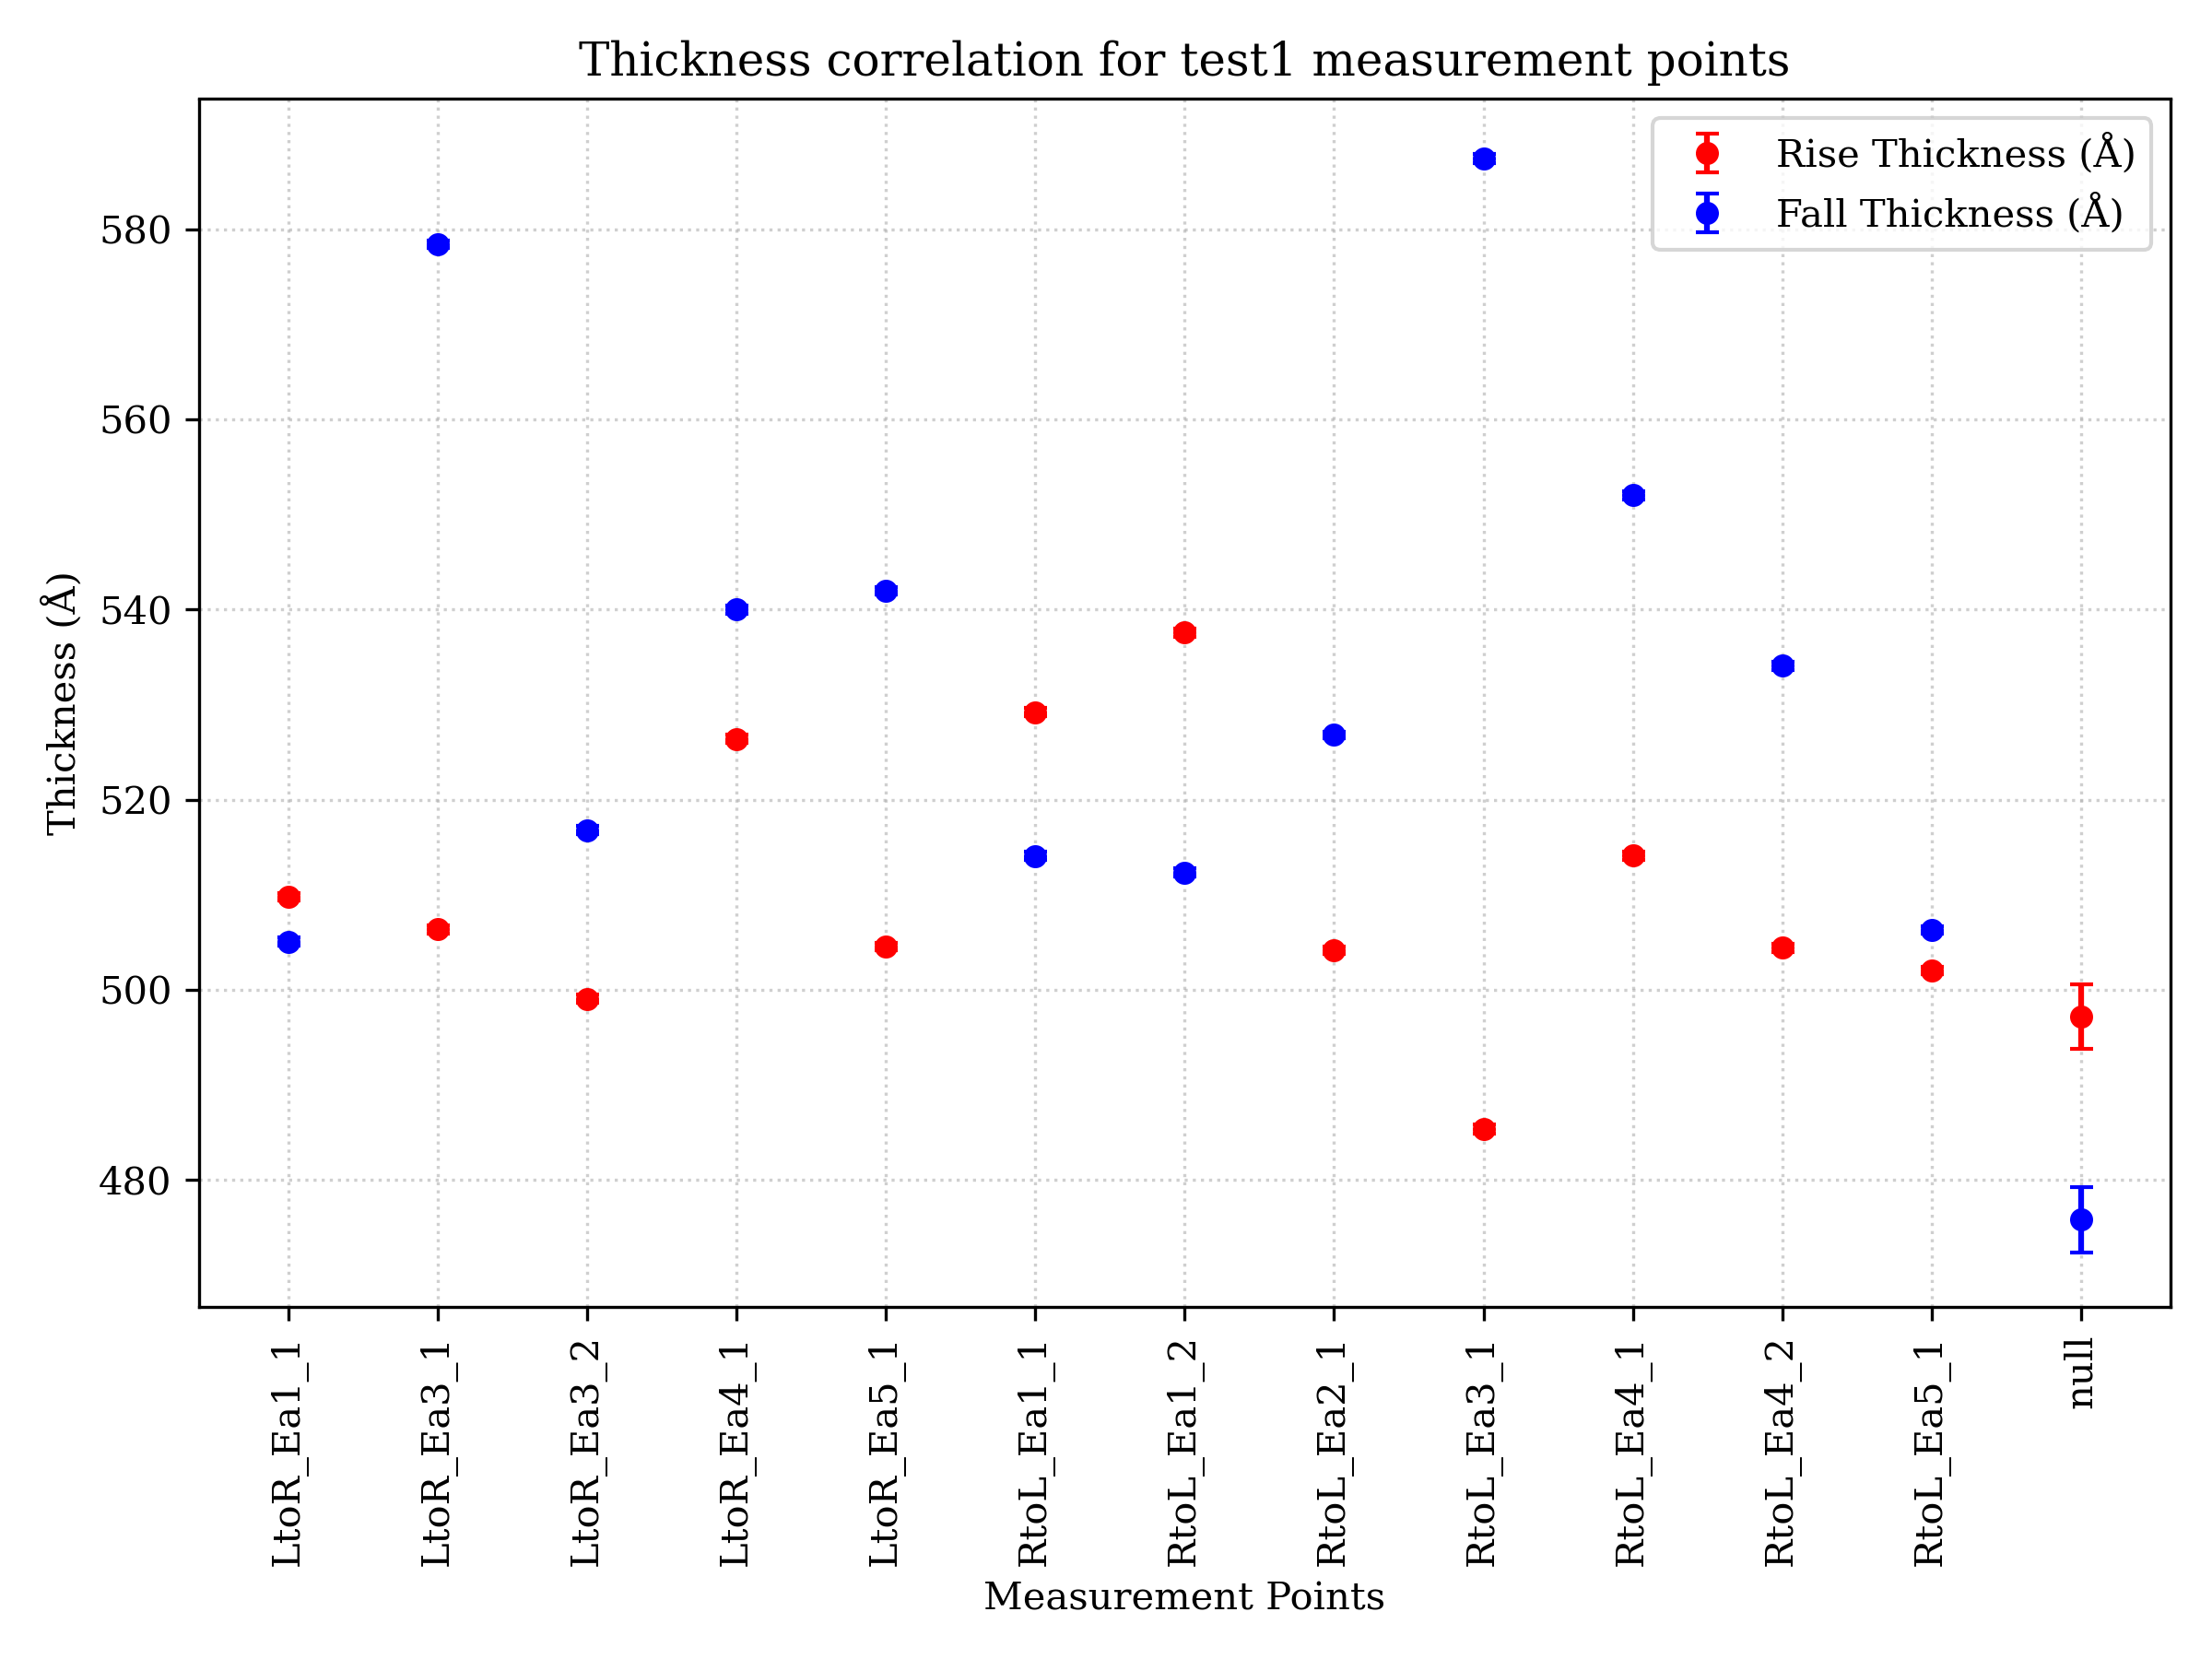
\includegraphics[width=0.8\textwidth]{thickness_correlation_test1.png}
    \label{fig:Correlationtest1}
\end{figure}
\begin{figure}[H]
    \centering
    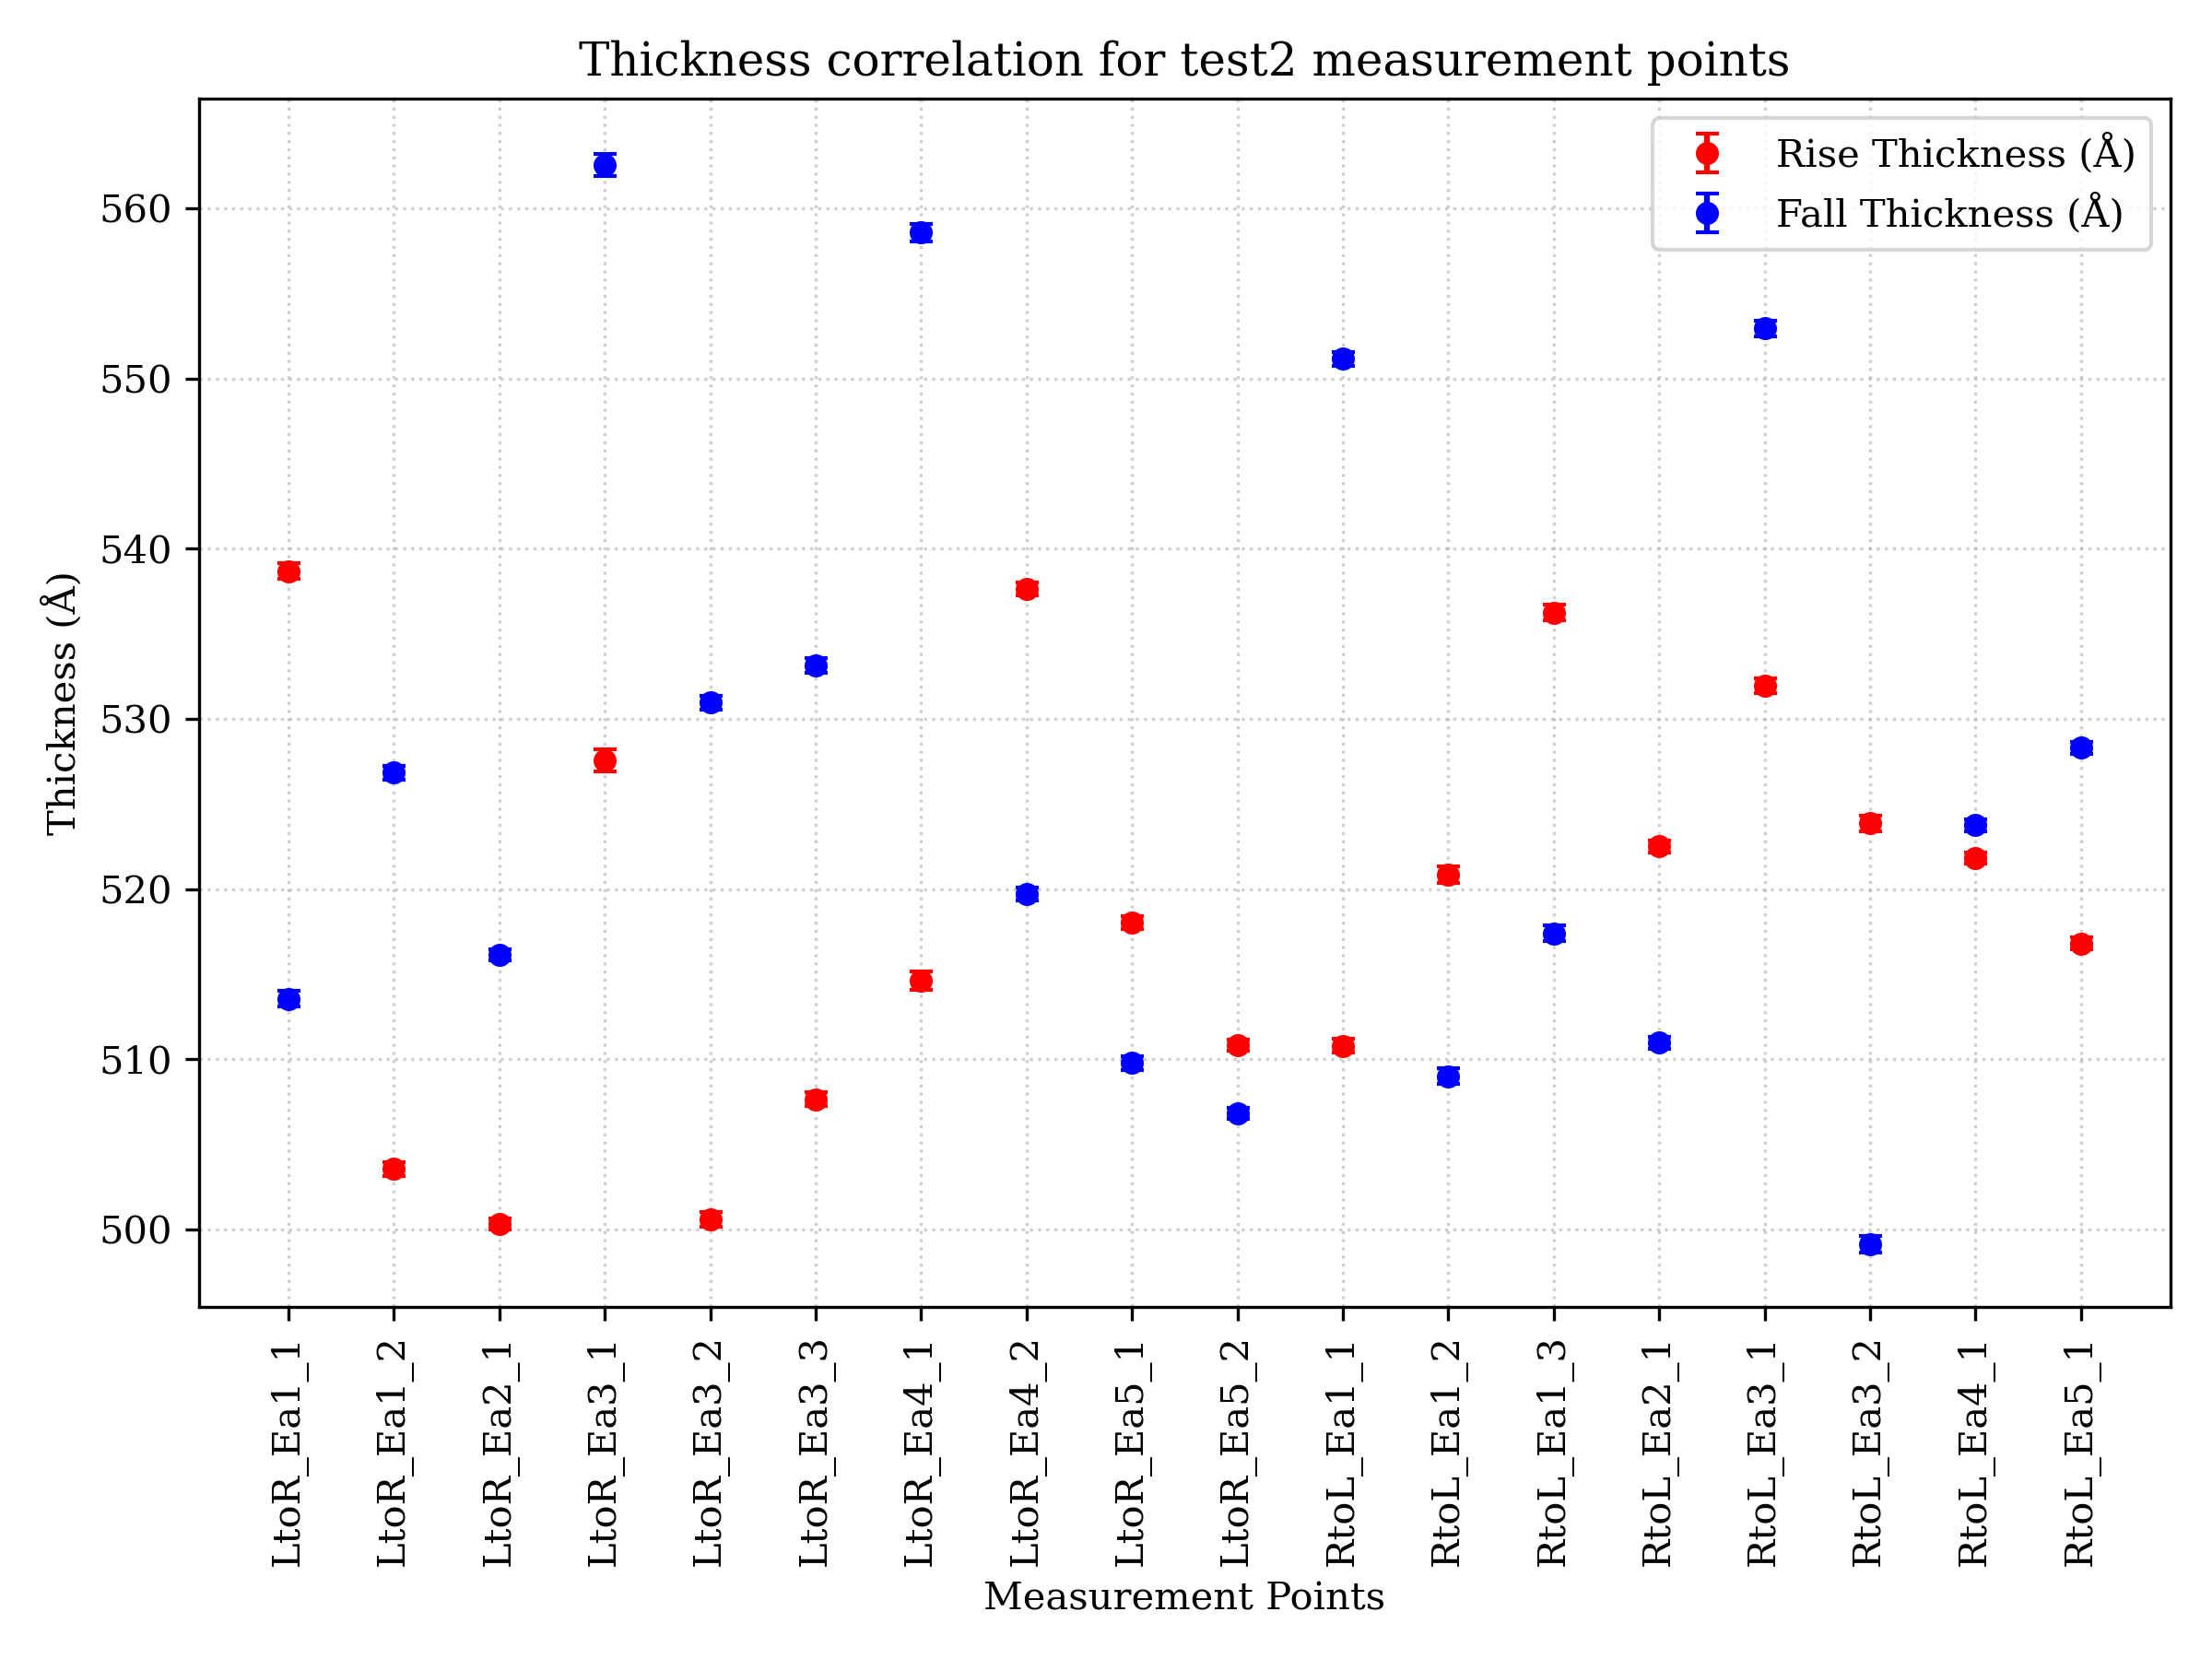
\includegraphics[width=0.8\textwidth]{thickness_correlation_test2.png}
    \label{fig:Correlationtest2}
\end{figure}
\begin{figure}[H]
    \centering
    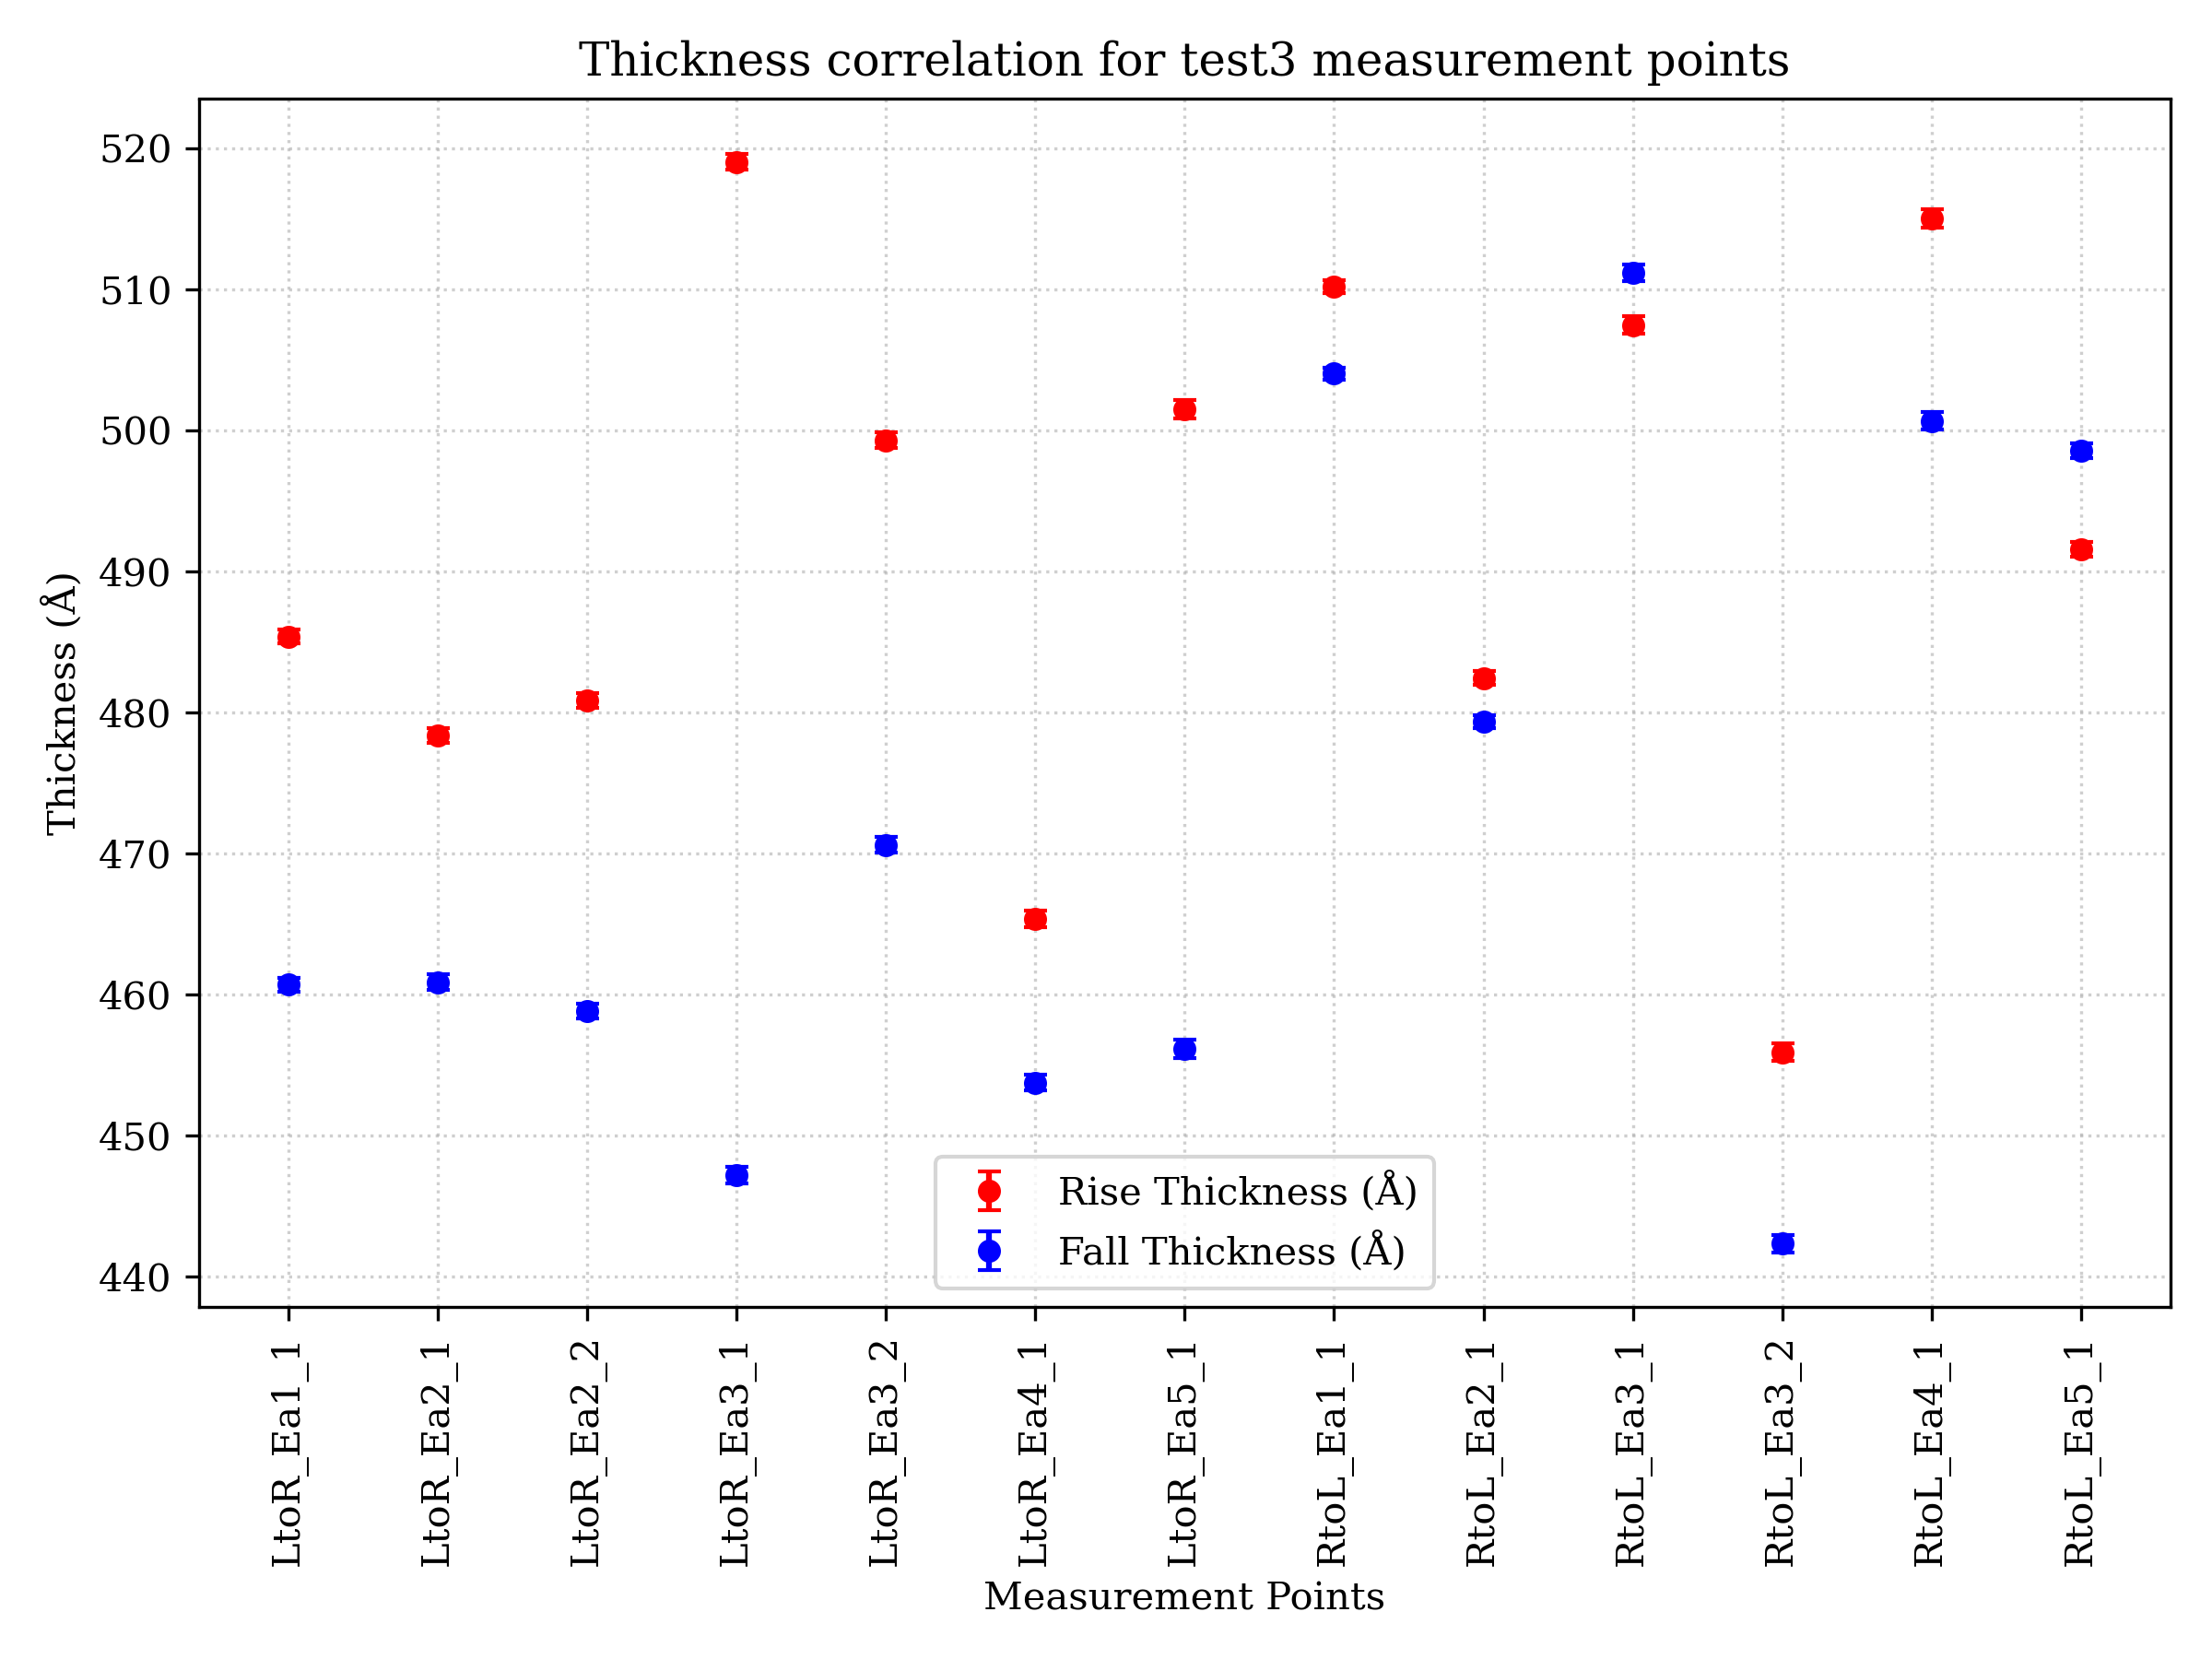
\includegraphics[width=0.8\textwidth]{thickness_correlation_test3.png}
    \label{fig:Correlationtest3}
\end{figure}
\clearpage

\section*{Each Plot}
全測定データを各々プロットする。
\par
横軸は測定位置のインデックスで,縦軸が膜厚値である。青色のラインは素データ,橙色のラインはuniform\_filter1dを用いてスムージングしたデータを表す。また,緑色のマーカーは立ち上がり始めの点,赤色のマーカーは立ち上がり終わりの点,シアン色のマーカーは立ち下がりは始めの点,マゼンタ色のマーカーは立ち下がり終わりの点を表す。
\begin{figure}[H]
    \centering
    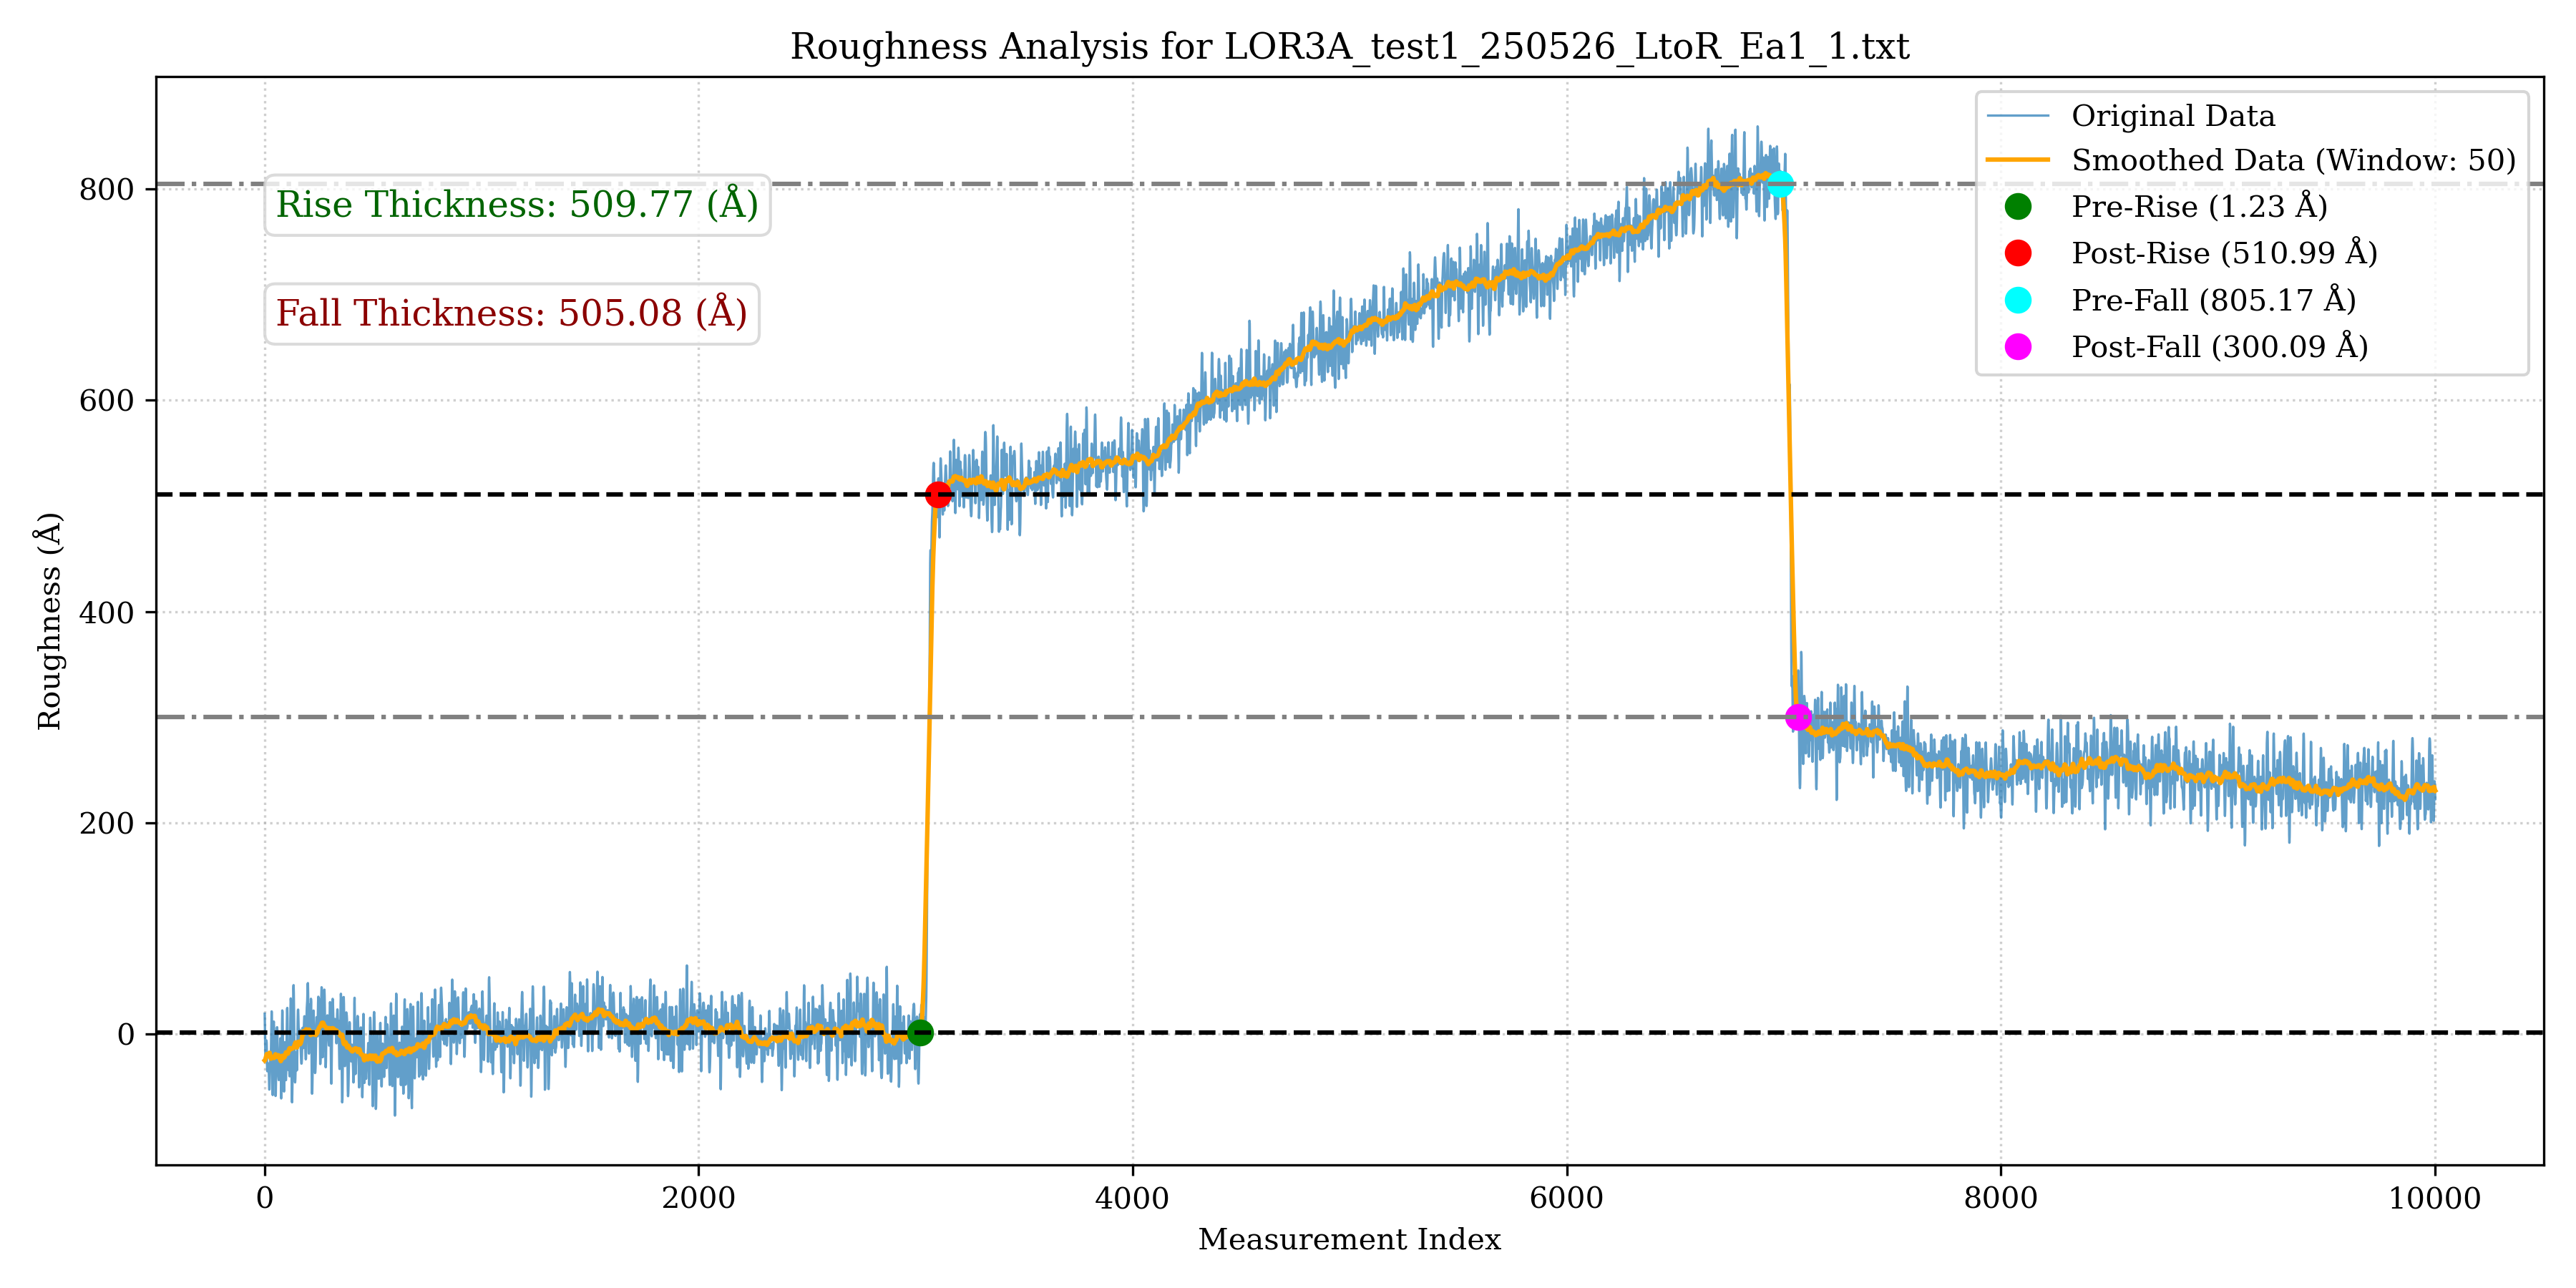
\includegraphics[width=\textwidth]{LOR3A_test1_250526_LtoR_Ea1_1.png}
    \label{fig:LOR3Atest1250526LtoREa11}
\end{figure}
\begin{figure}[H]
    \centering
    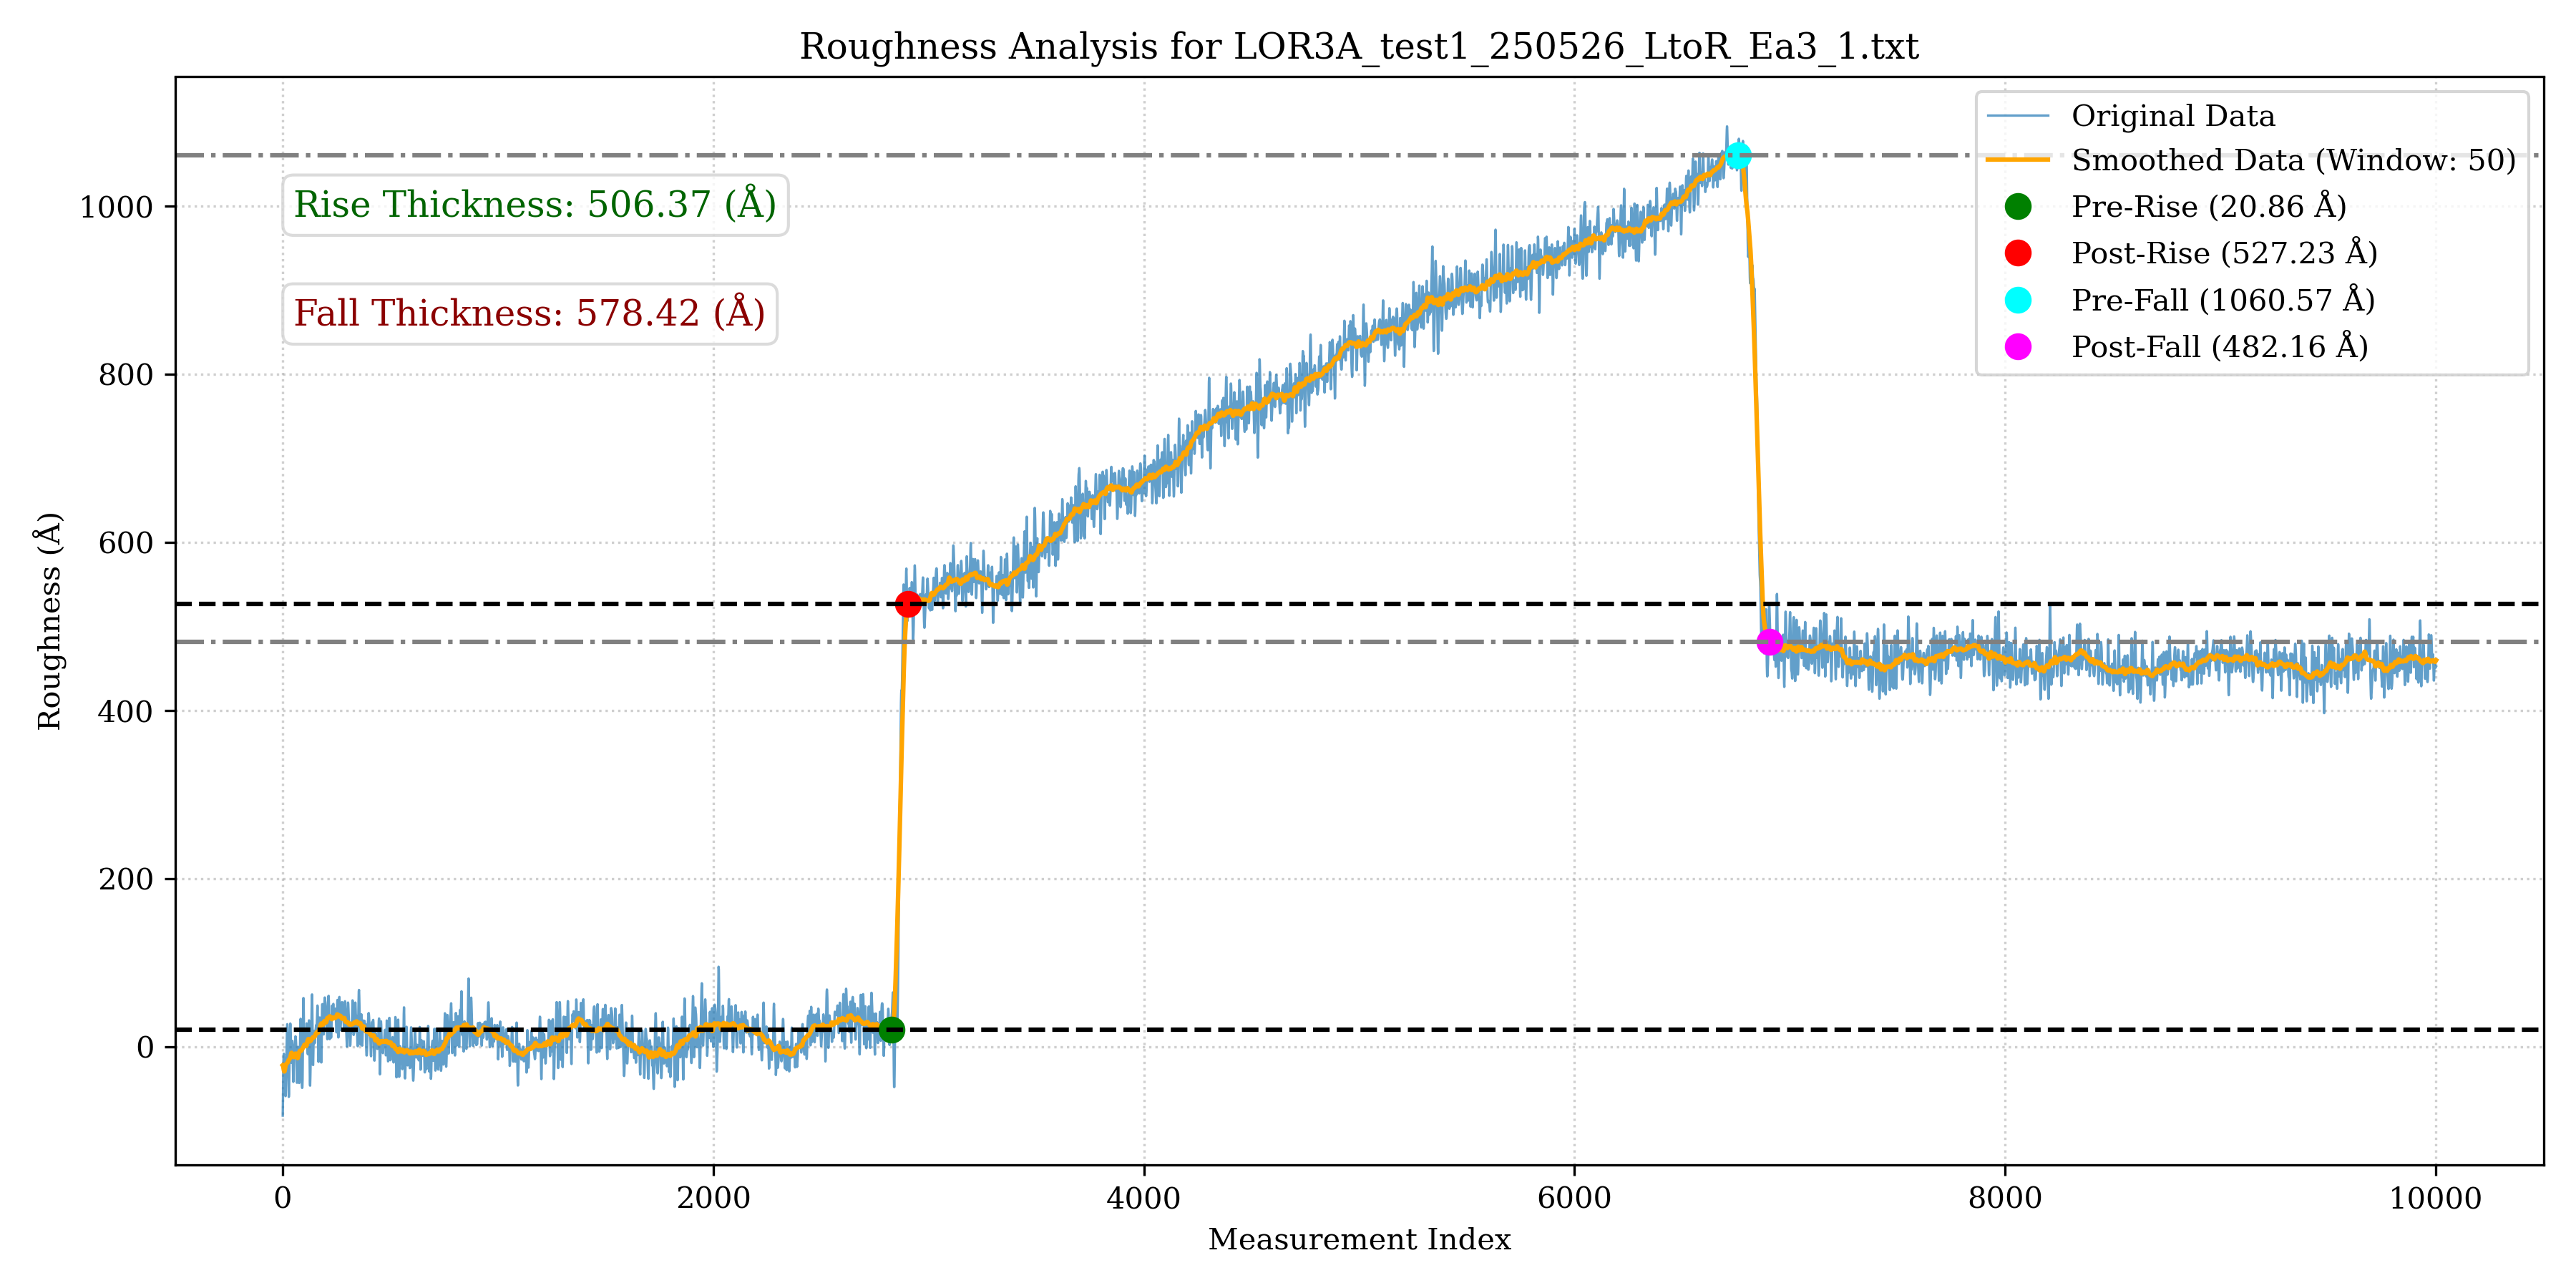
\includegraphics[width=\textwidth]{LOR3A_test1_250526_LtoR_Ea3_1.png}
    \label{fig:LOR3Atest1250526LtoREa31}
\end{figure}
\begin{figure}[H]
    \centering
    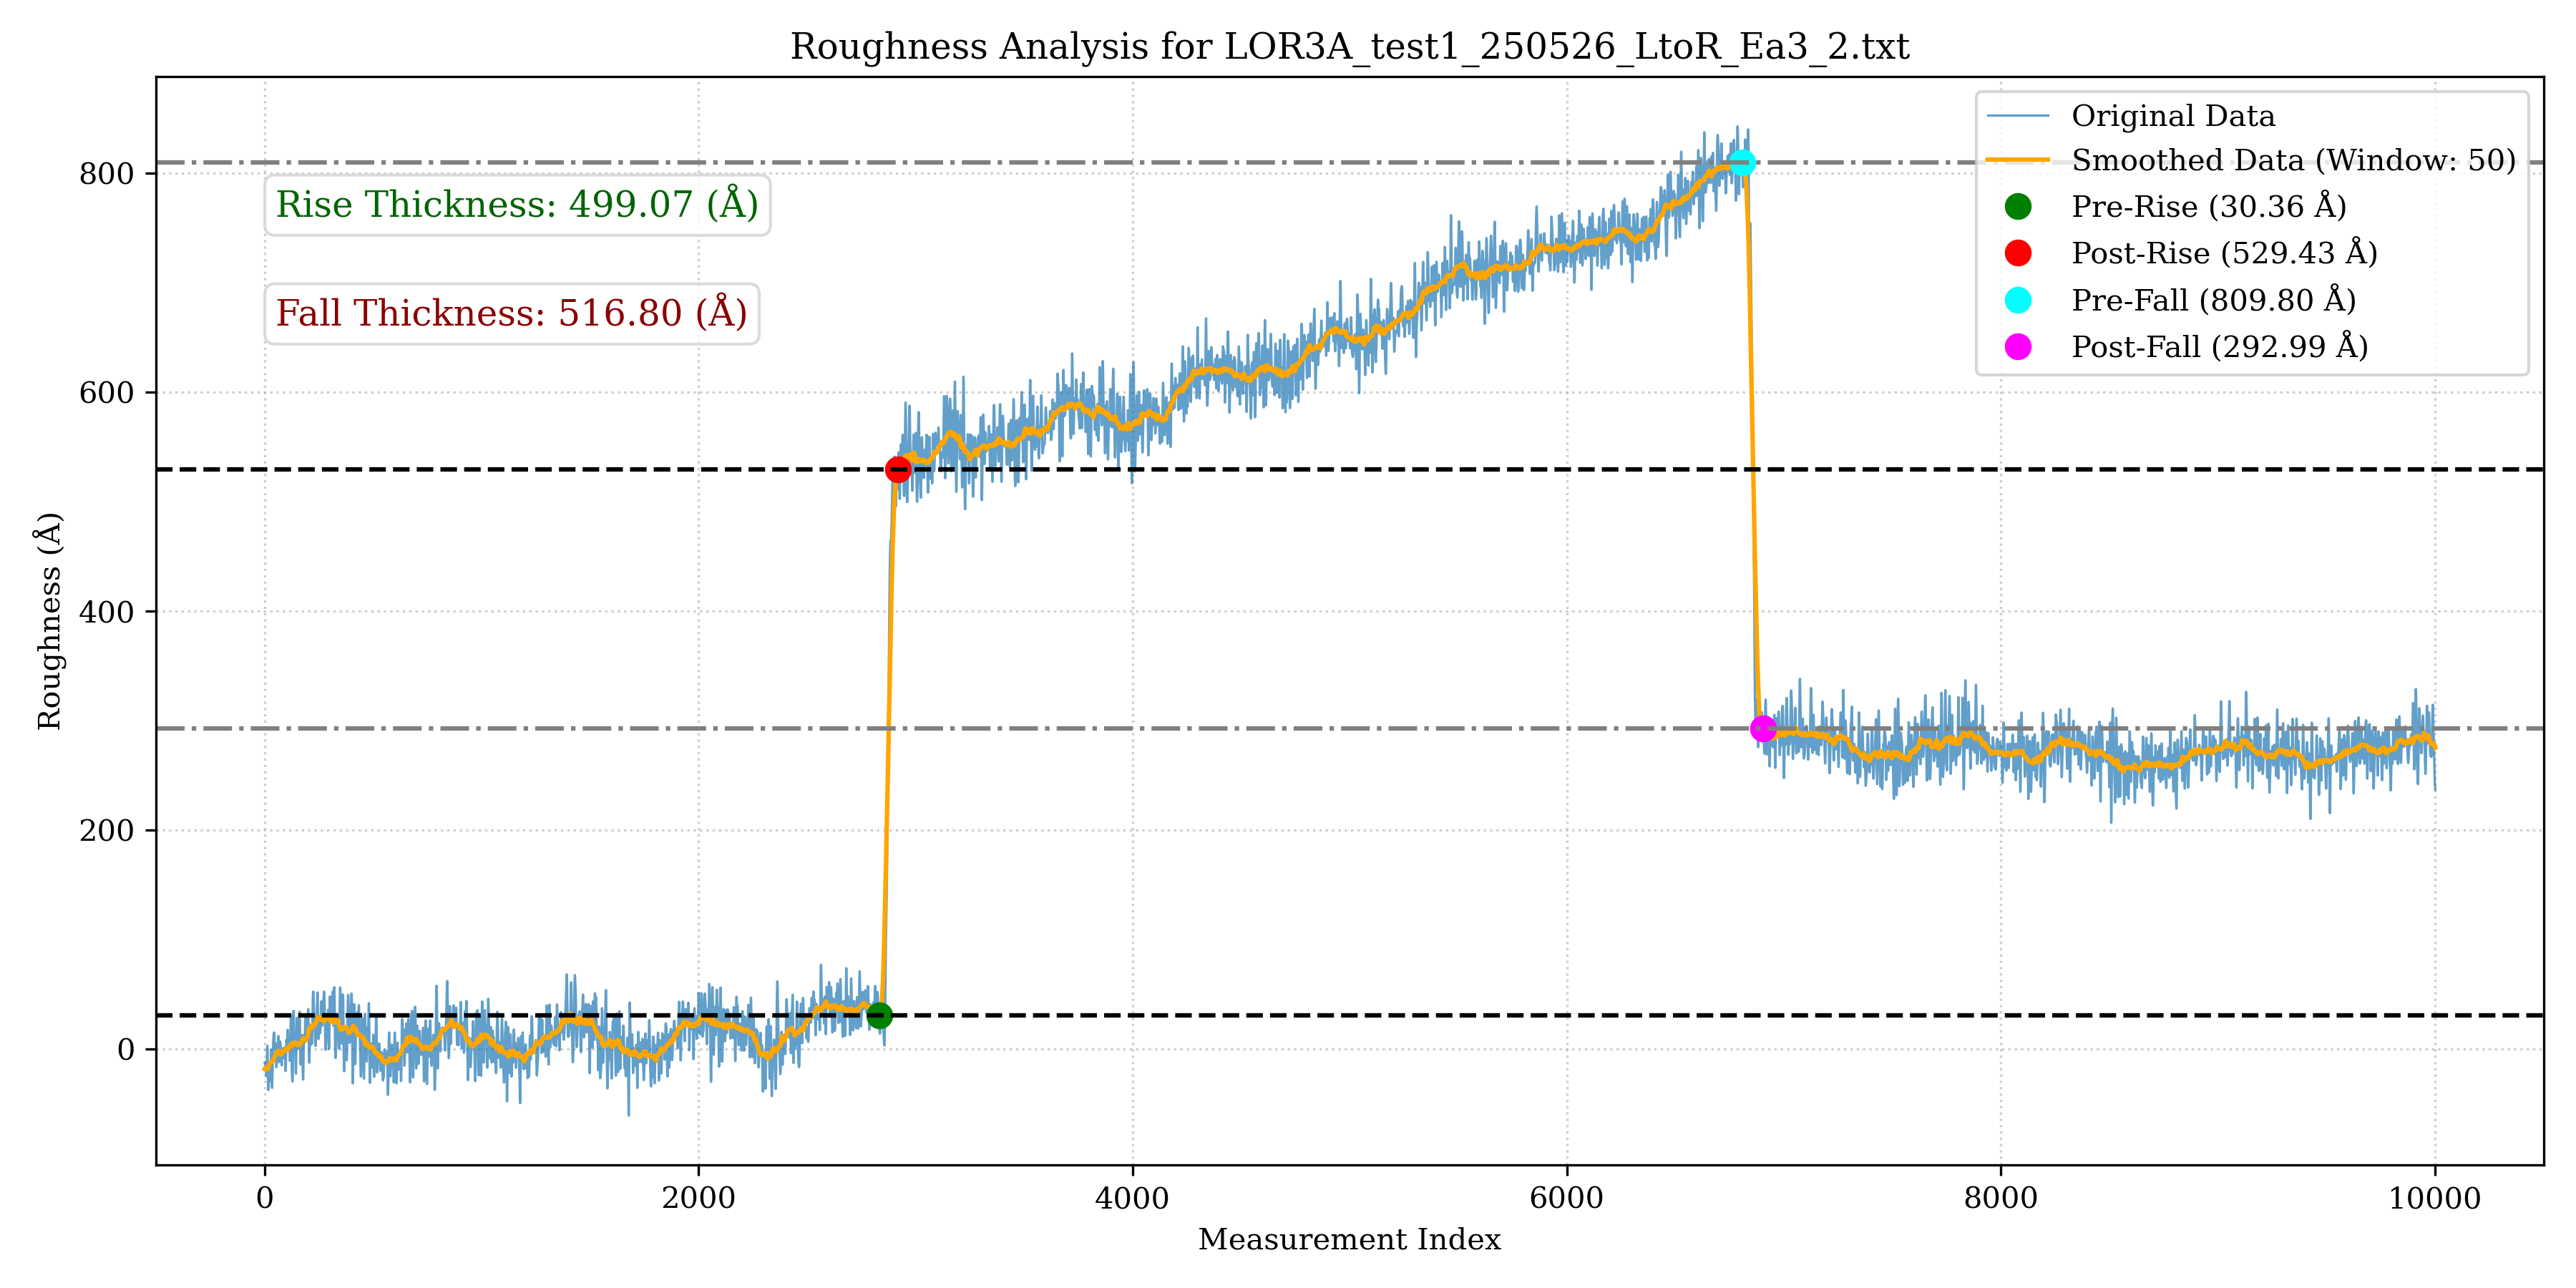
\includegraphics[width=\textwidth]{LOR3A_test1_250526_LtoR_Ea3_2.png}
    \label{fig:LOR3Atest1250526LtoREa32}
\end{figure}
\begin{figure}[H]
    \centering
    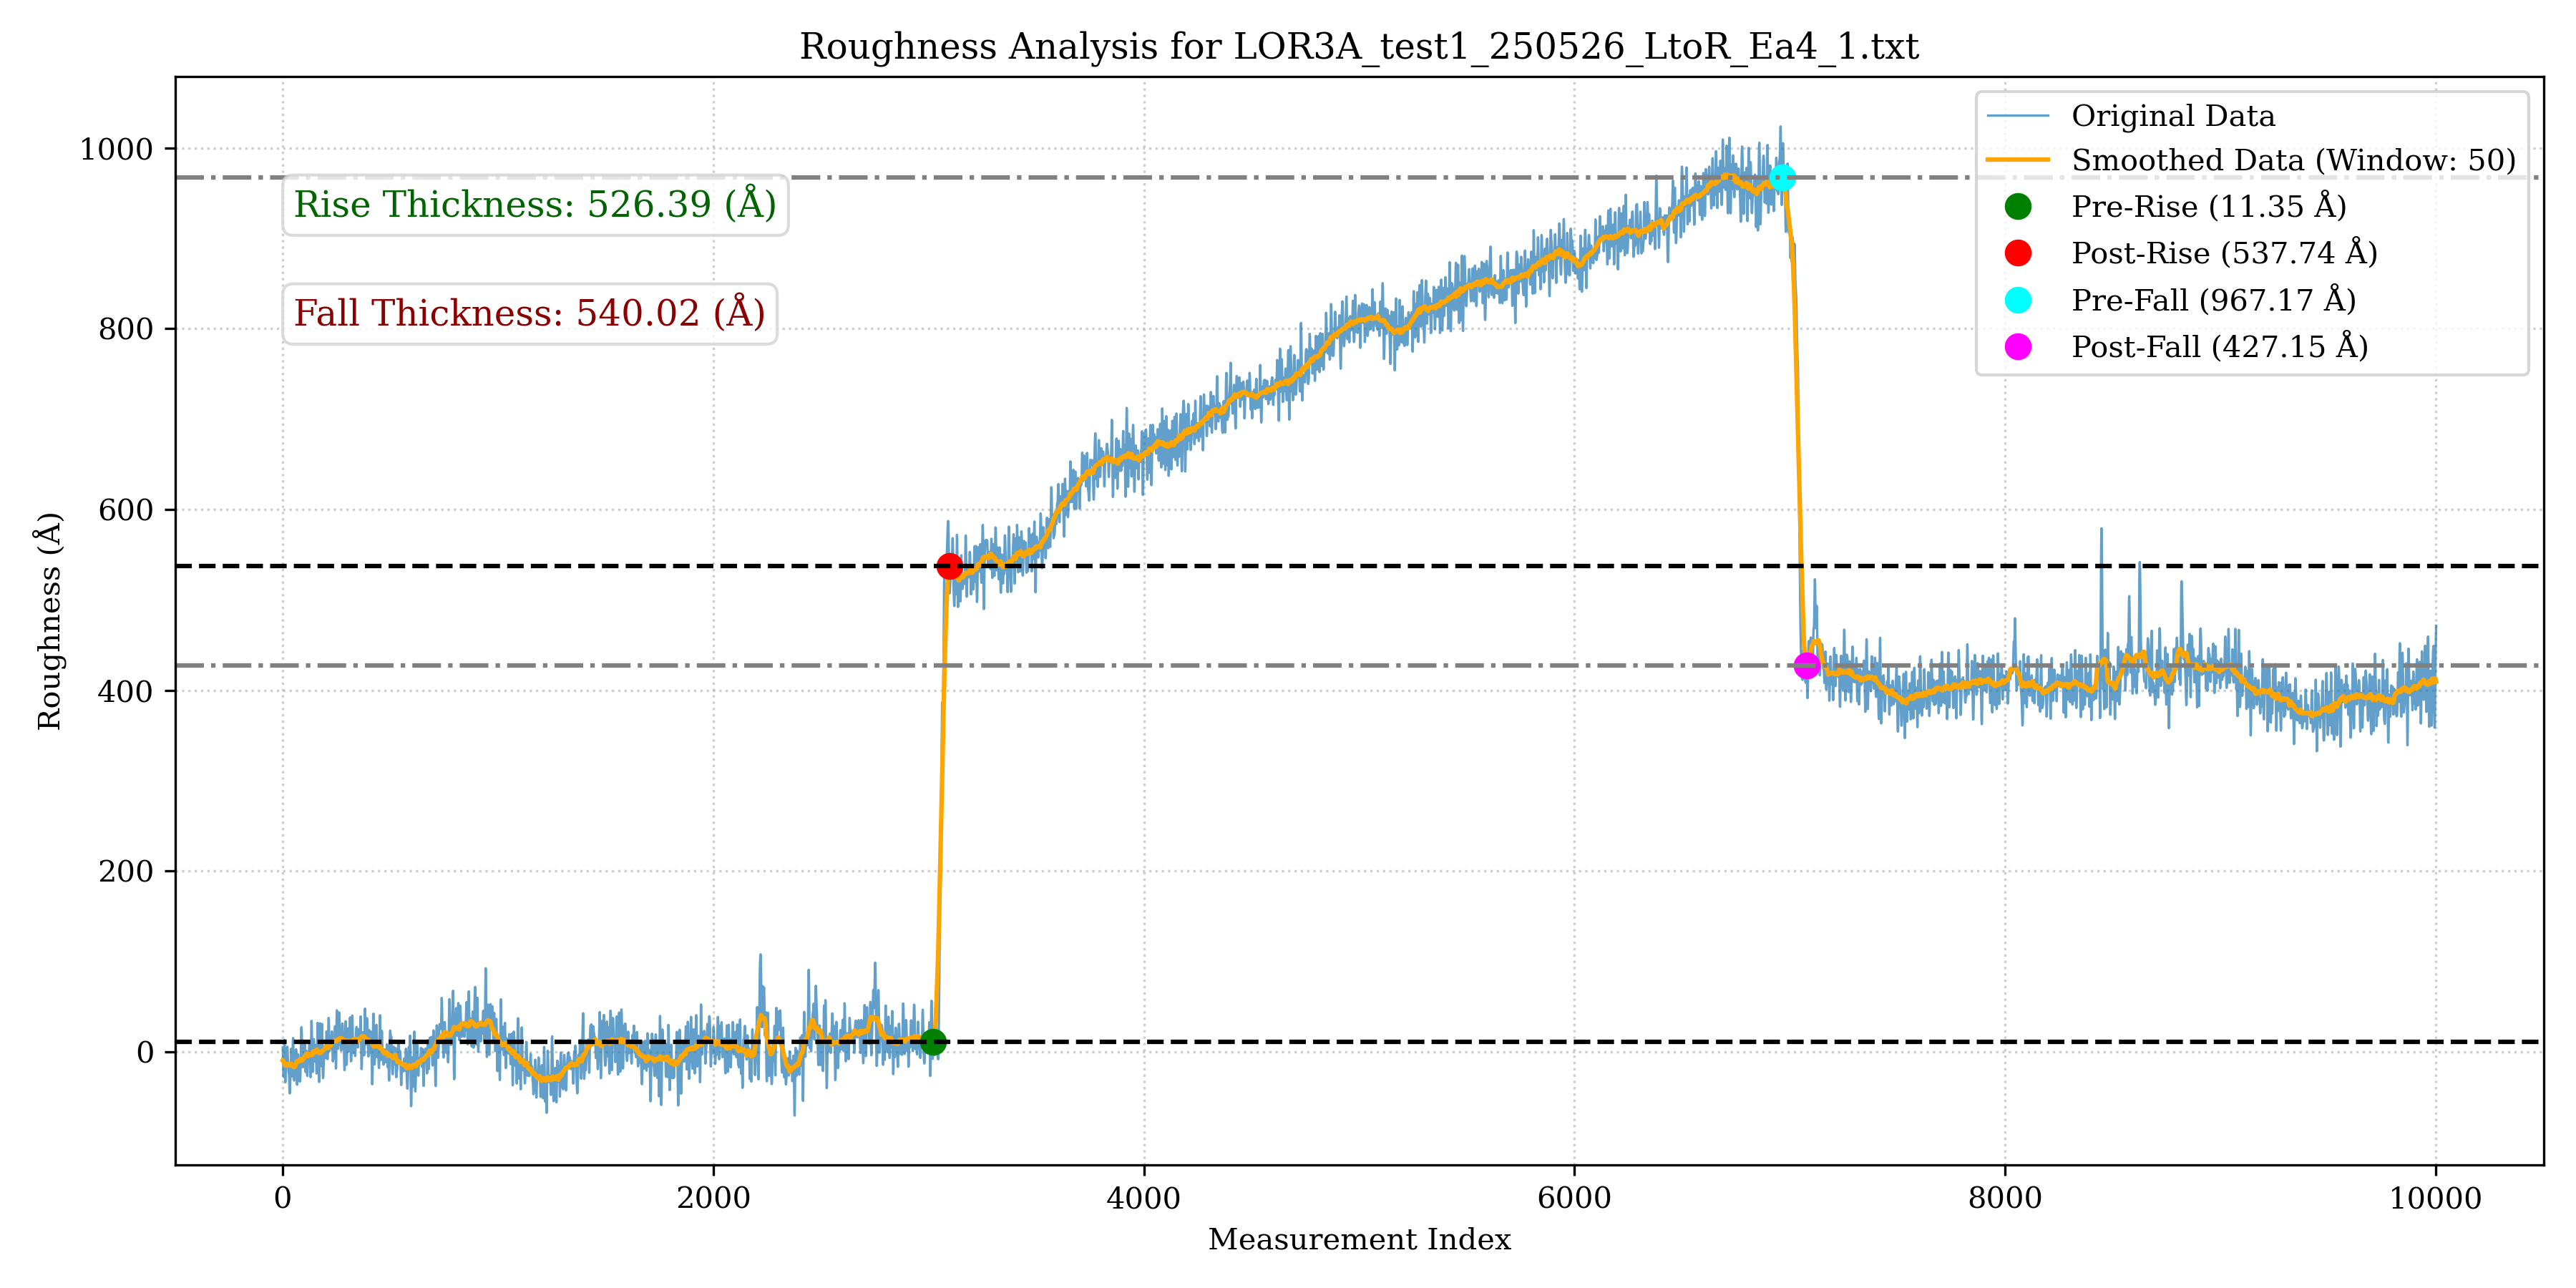
\includegraphics[width=\textwidth]{LOR3A_test1_250526_LtoR_Ea4_1.png}
    \label{fig:LOR3Atest1250526LtoREa41}
\end{figure}
\begin{figure}[H]
    \centering
    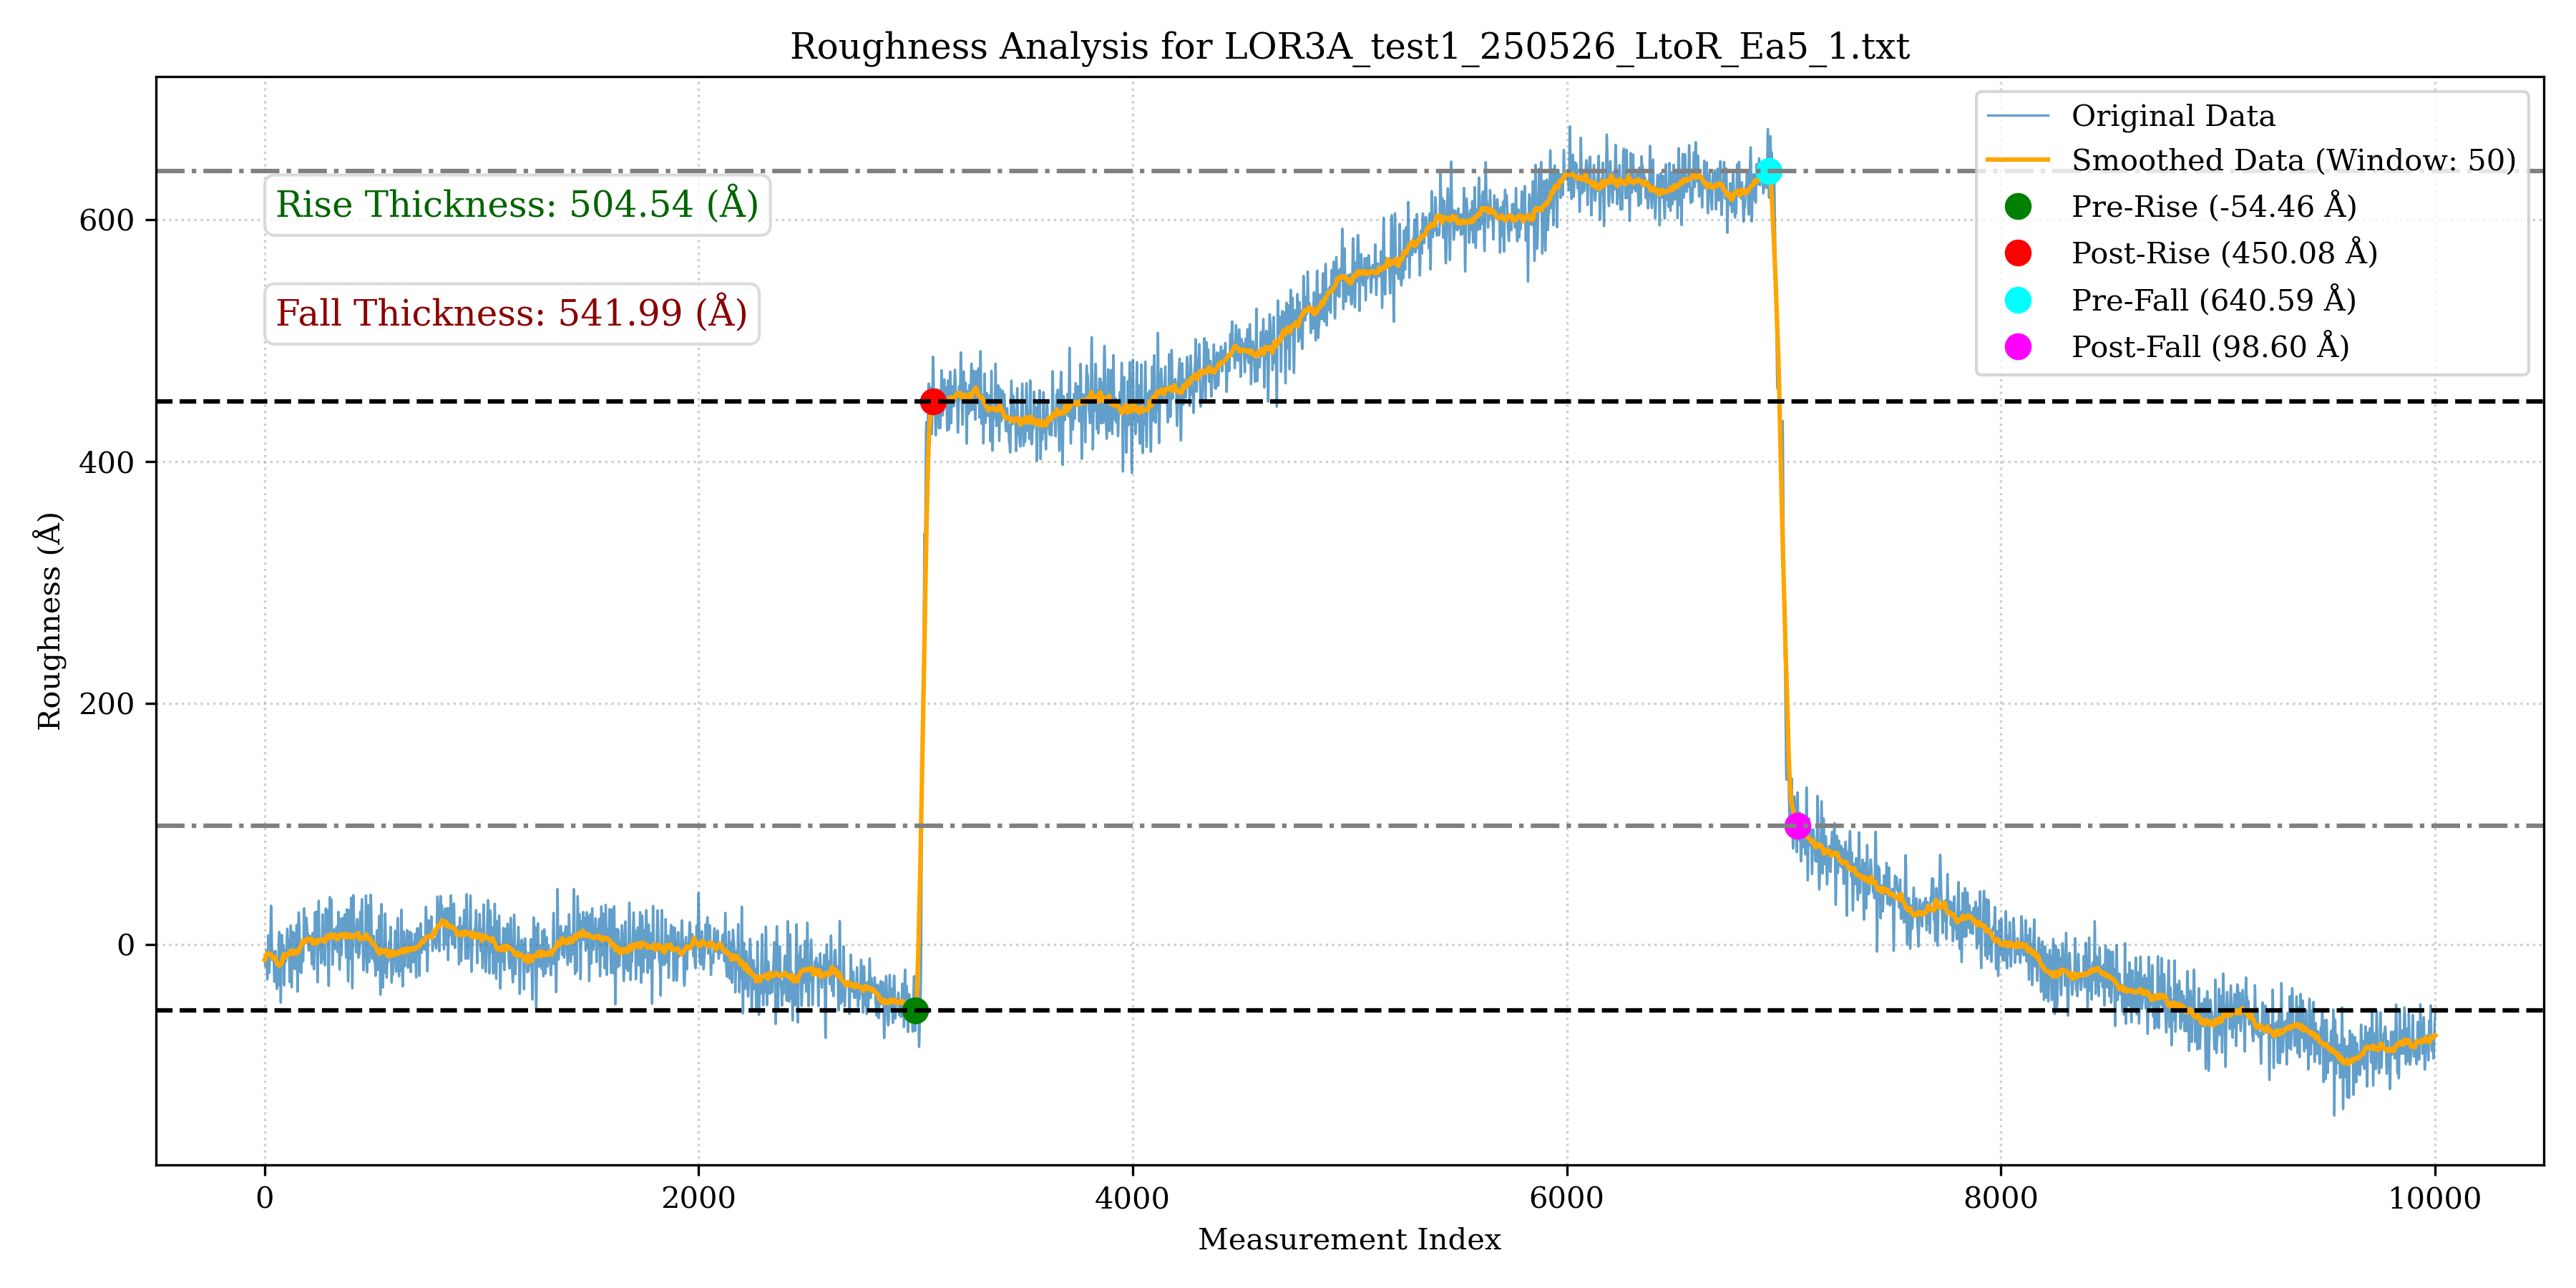
\includegraphics[width=\textwidth]{LOR3A_test1_250526_LtoR_Ea5_1.png}
    \label{fig:LOR3Atest1250526LtoREa51}
\end{figure}
\begin{figure}[H]
    \centering
    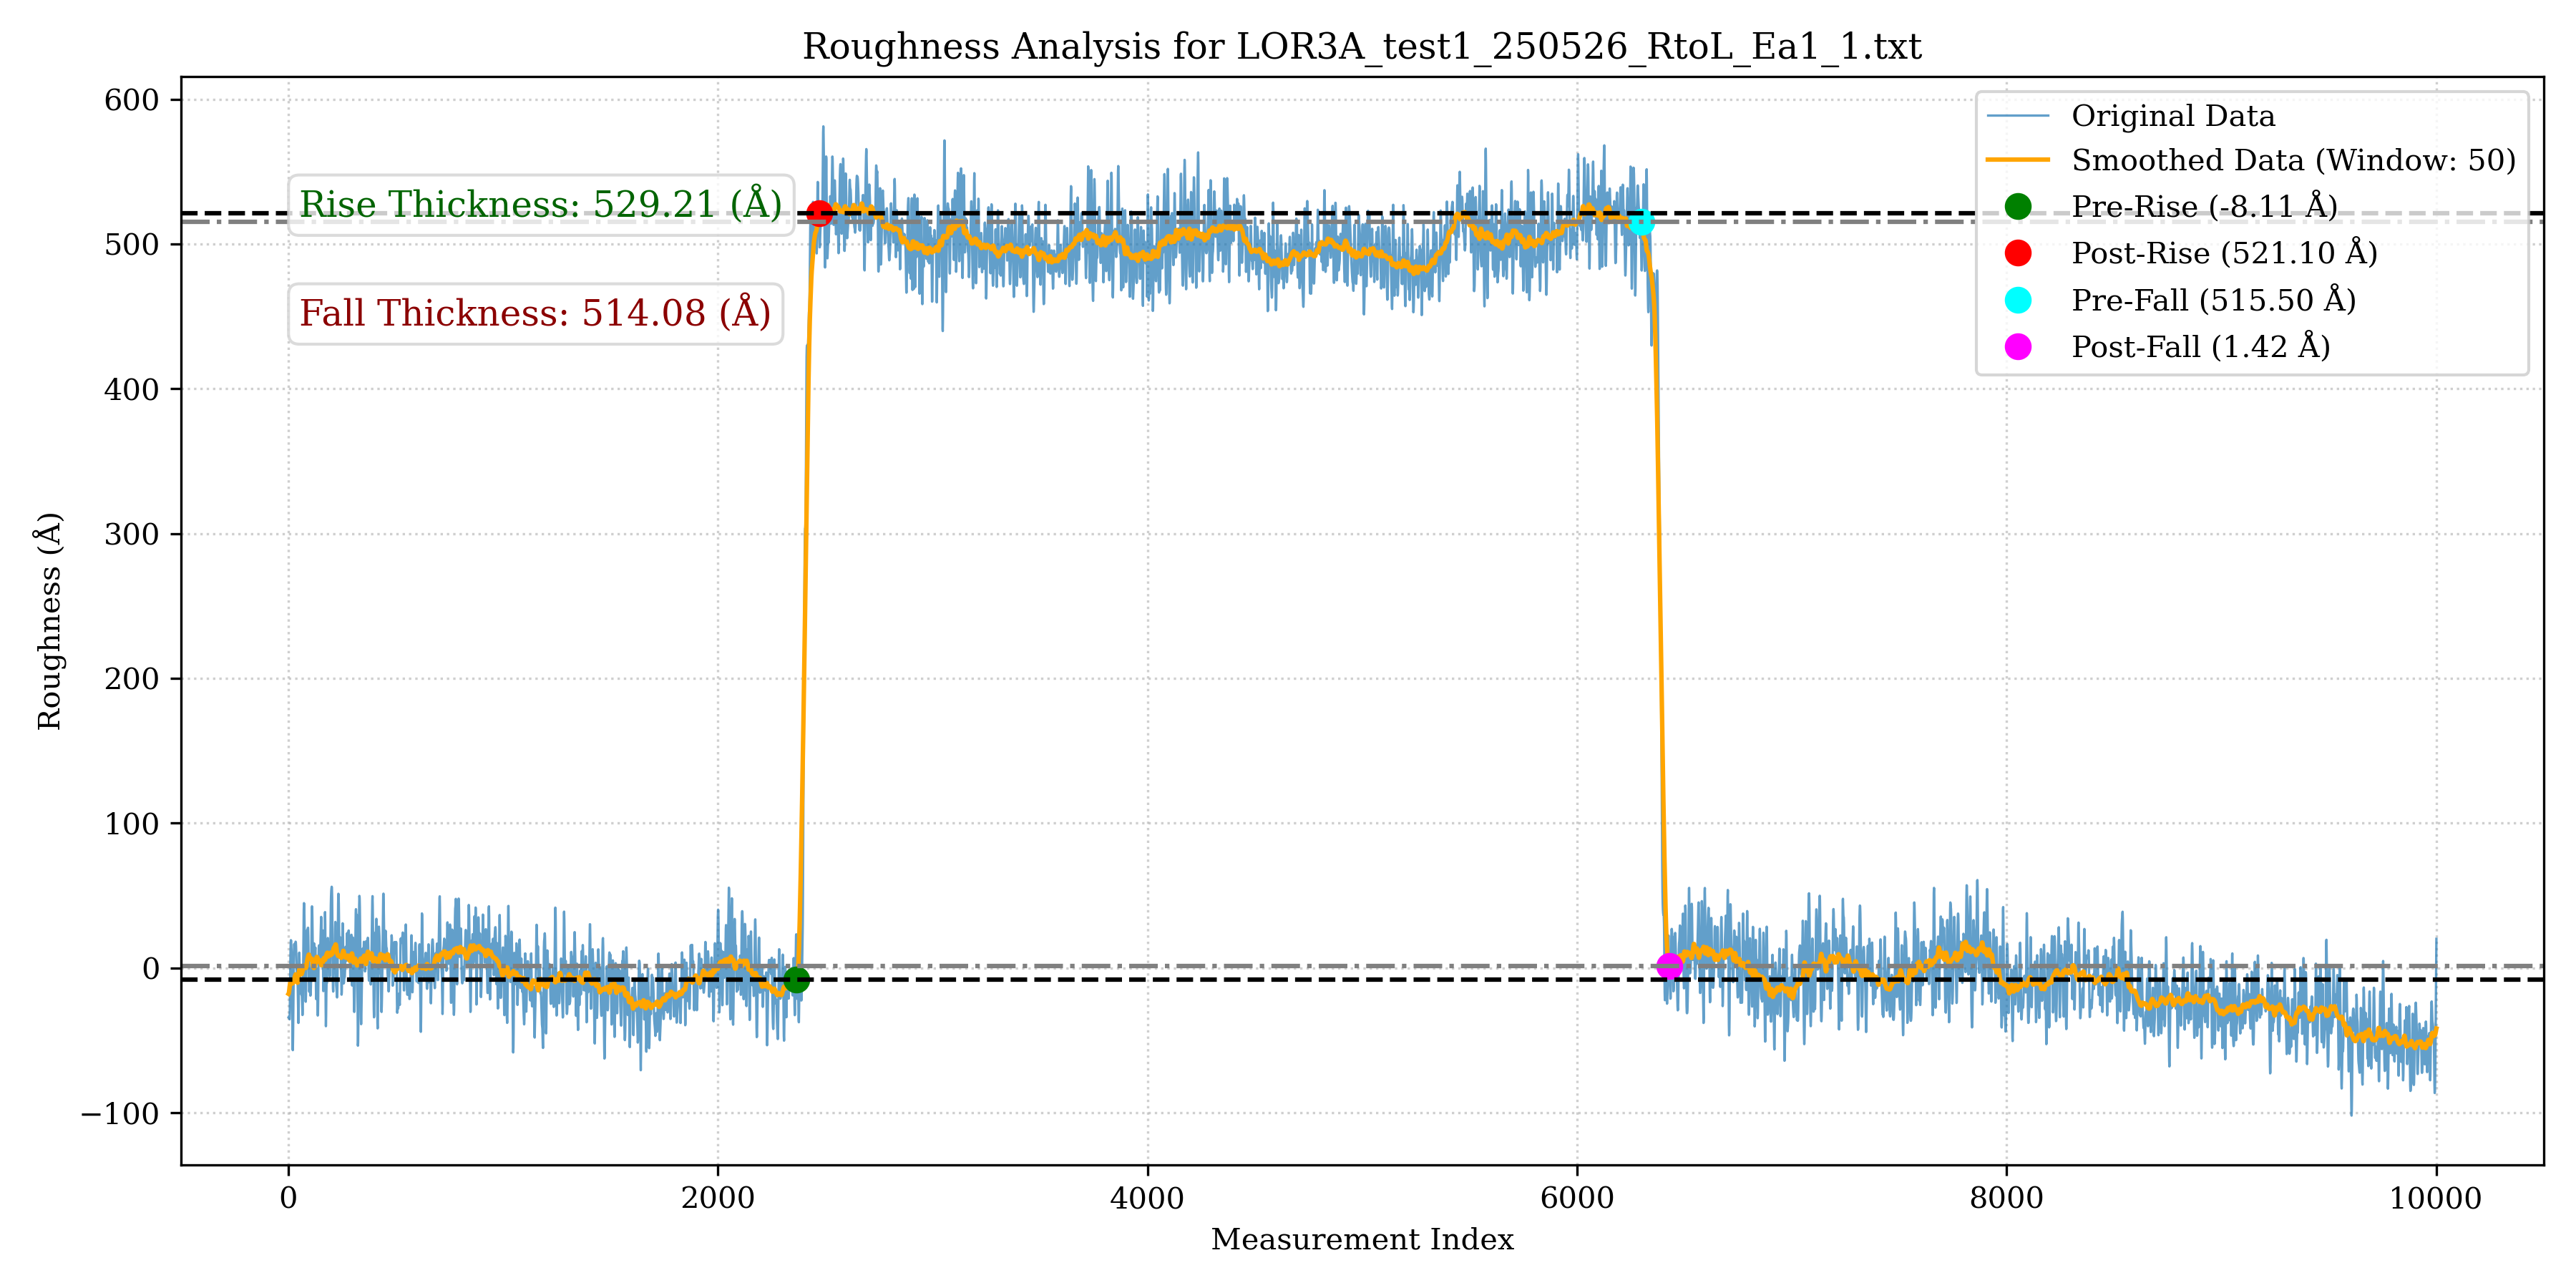
\includegraphics[width=\textwidth]{LOR3A_test1_250526_RtoL_Ea1_1.png}
    \label{fig:LOR3Atest1250526RtoLEa11}
\end{figure}
\begin{figure}[H]
    \centering
    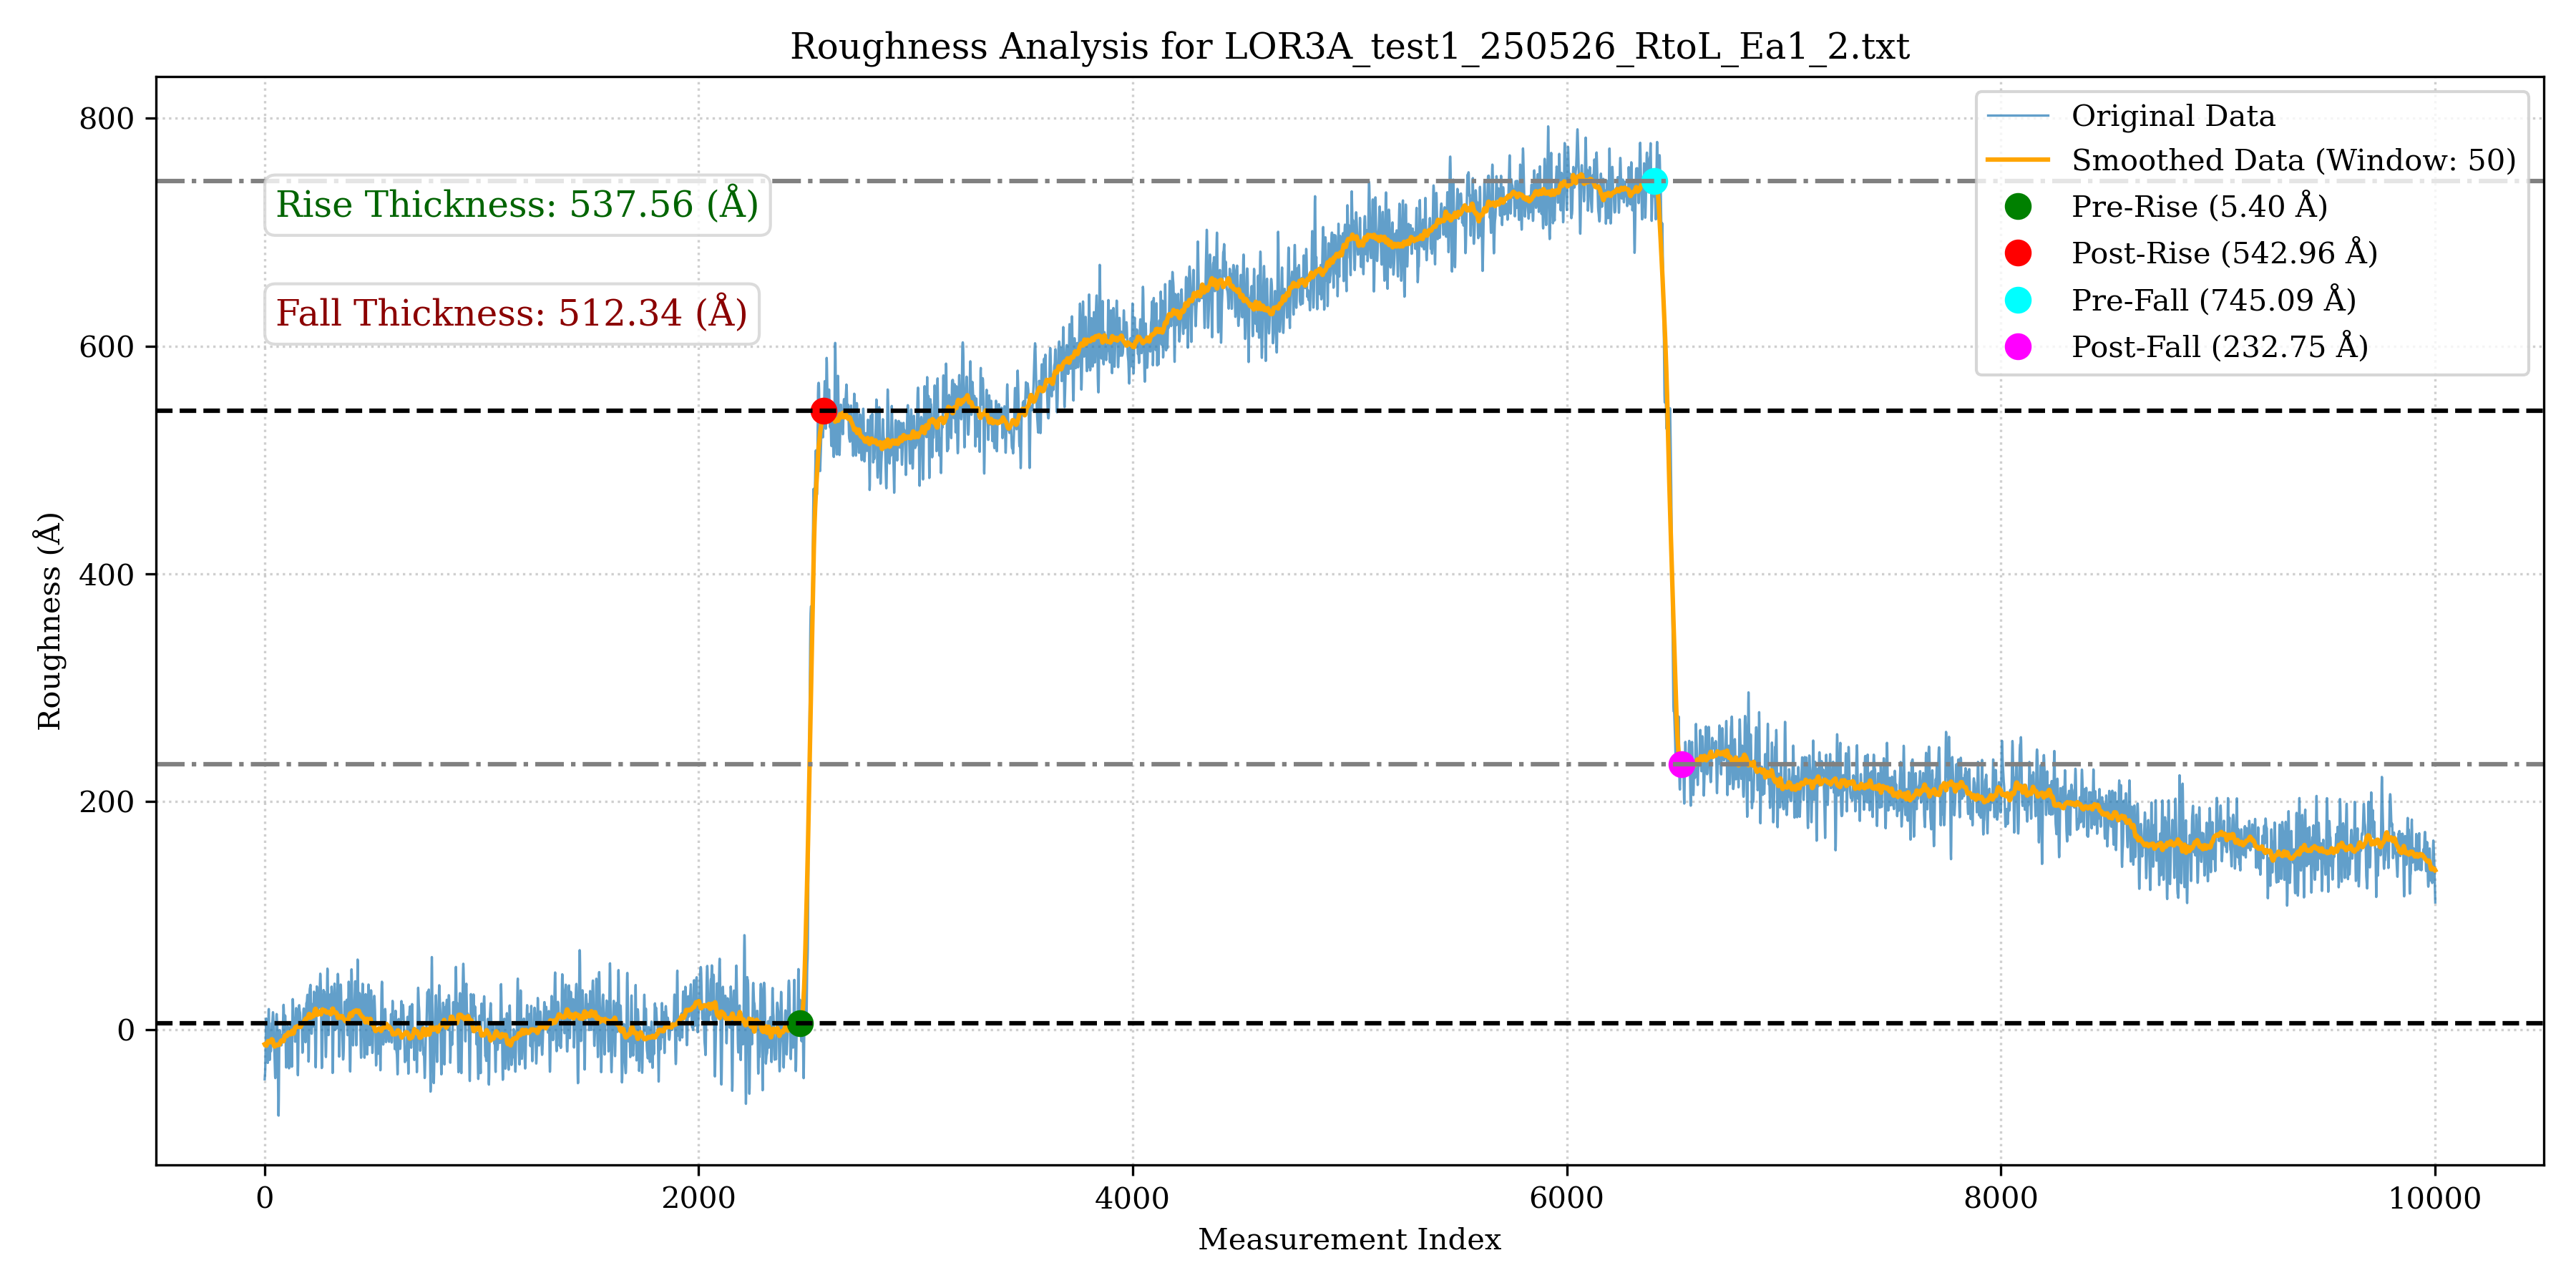
\includegraphics[width=\textwidth]{LOR3A_test1_250526_RtoL_Ea1_2.png}
    \label{fig:LOR3Atest1250526RtoLEa12}
\end{figure}
\begin{figure}[H]
    \centering
    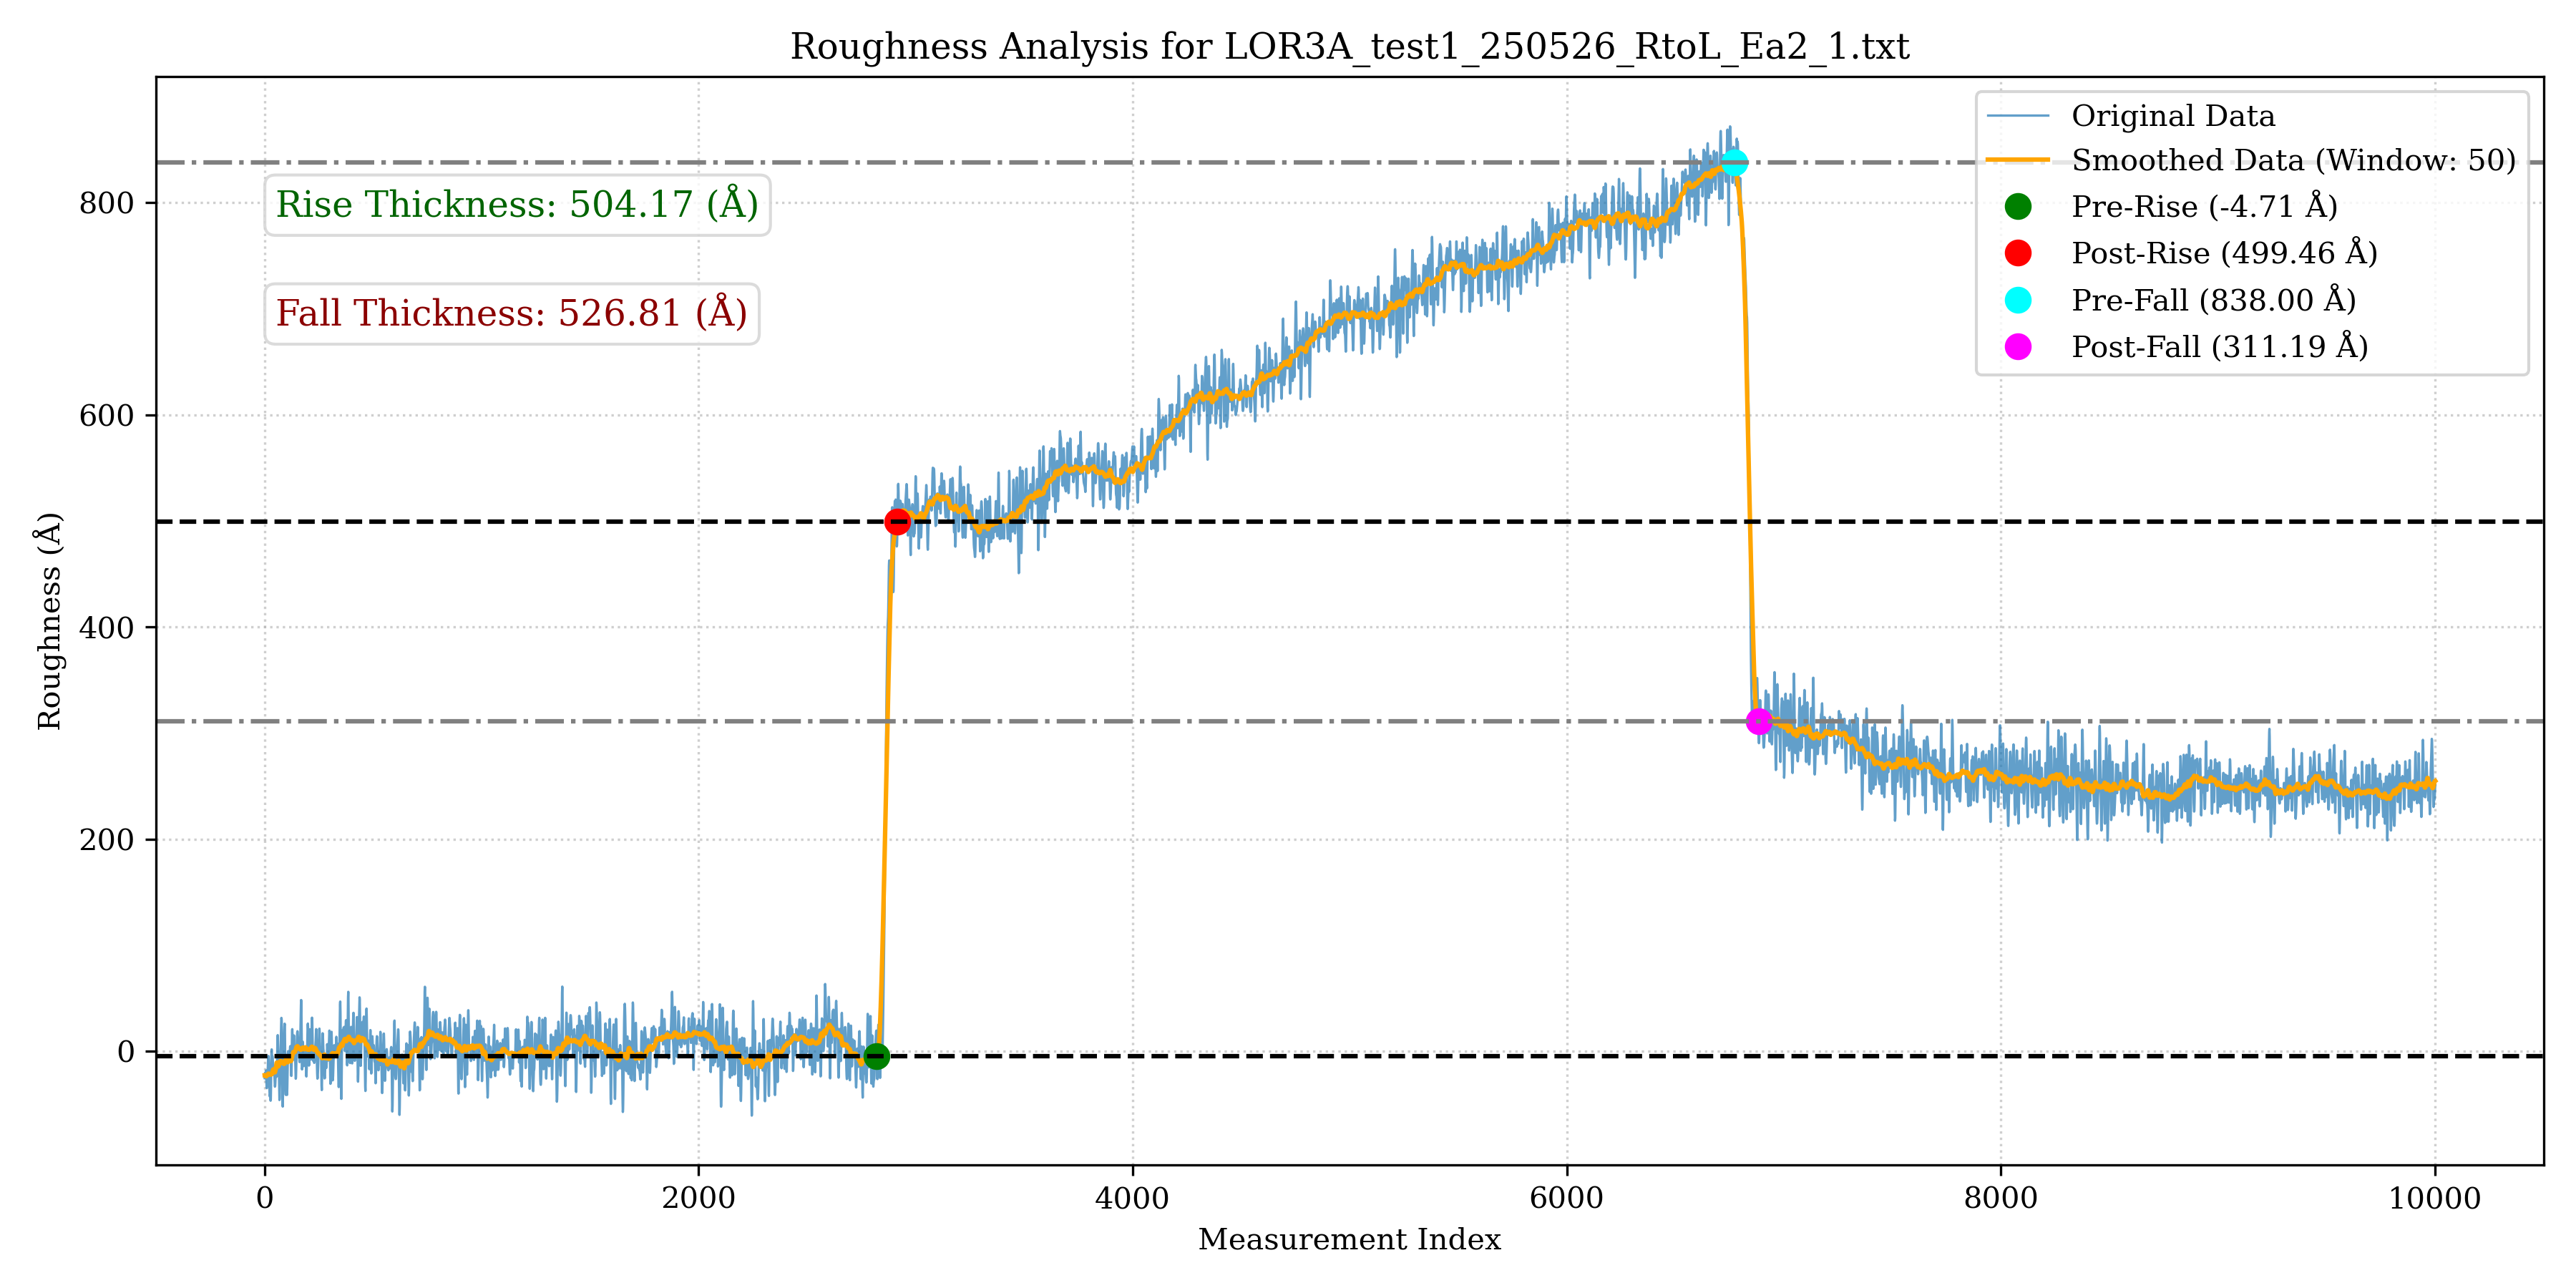
\includegraphics[width=\textwidth]{LOR3A_test1_250526_RtoL_Ea2_1.png}
    \label{fig:LOR3Atest1250526RtoLEa21}
\end{figure}
\begin{figure}[H]
    \centering
    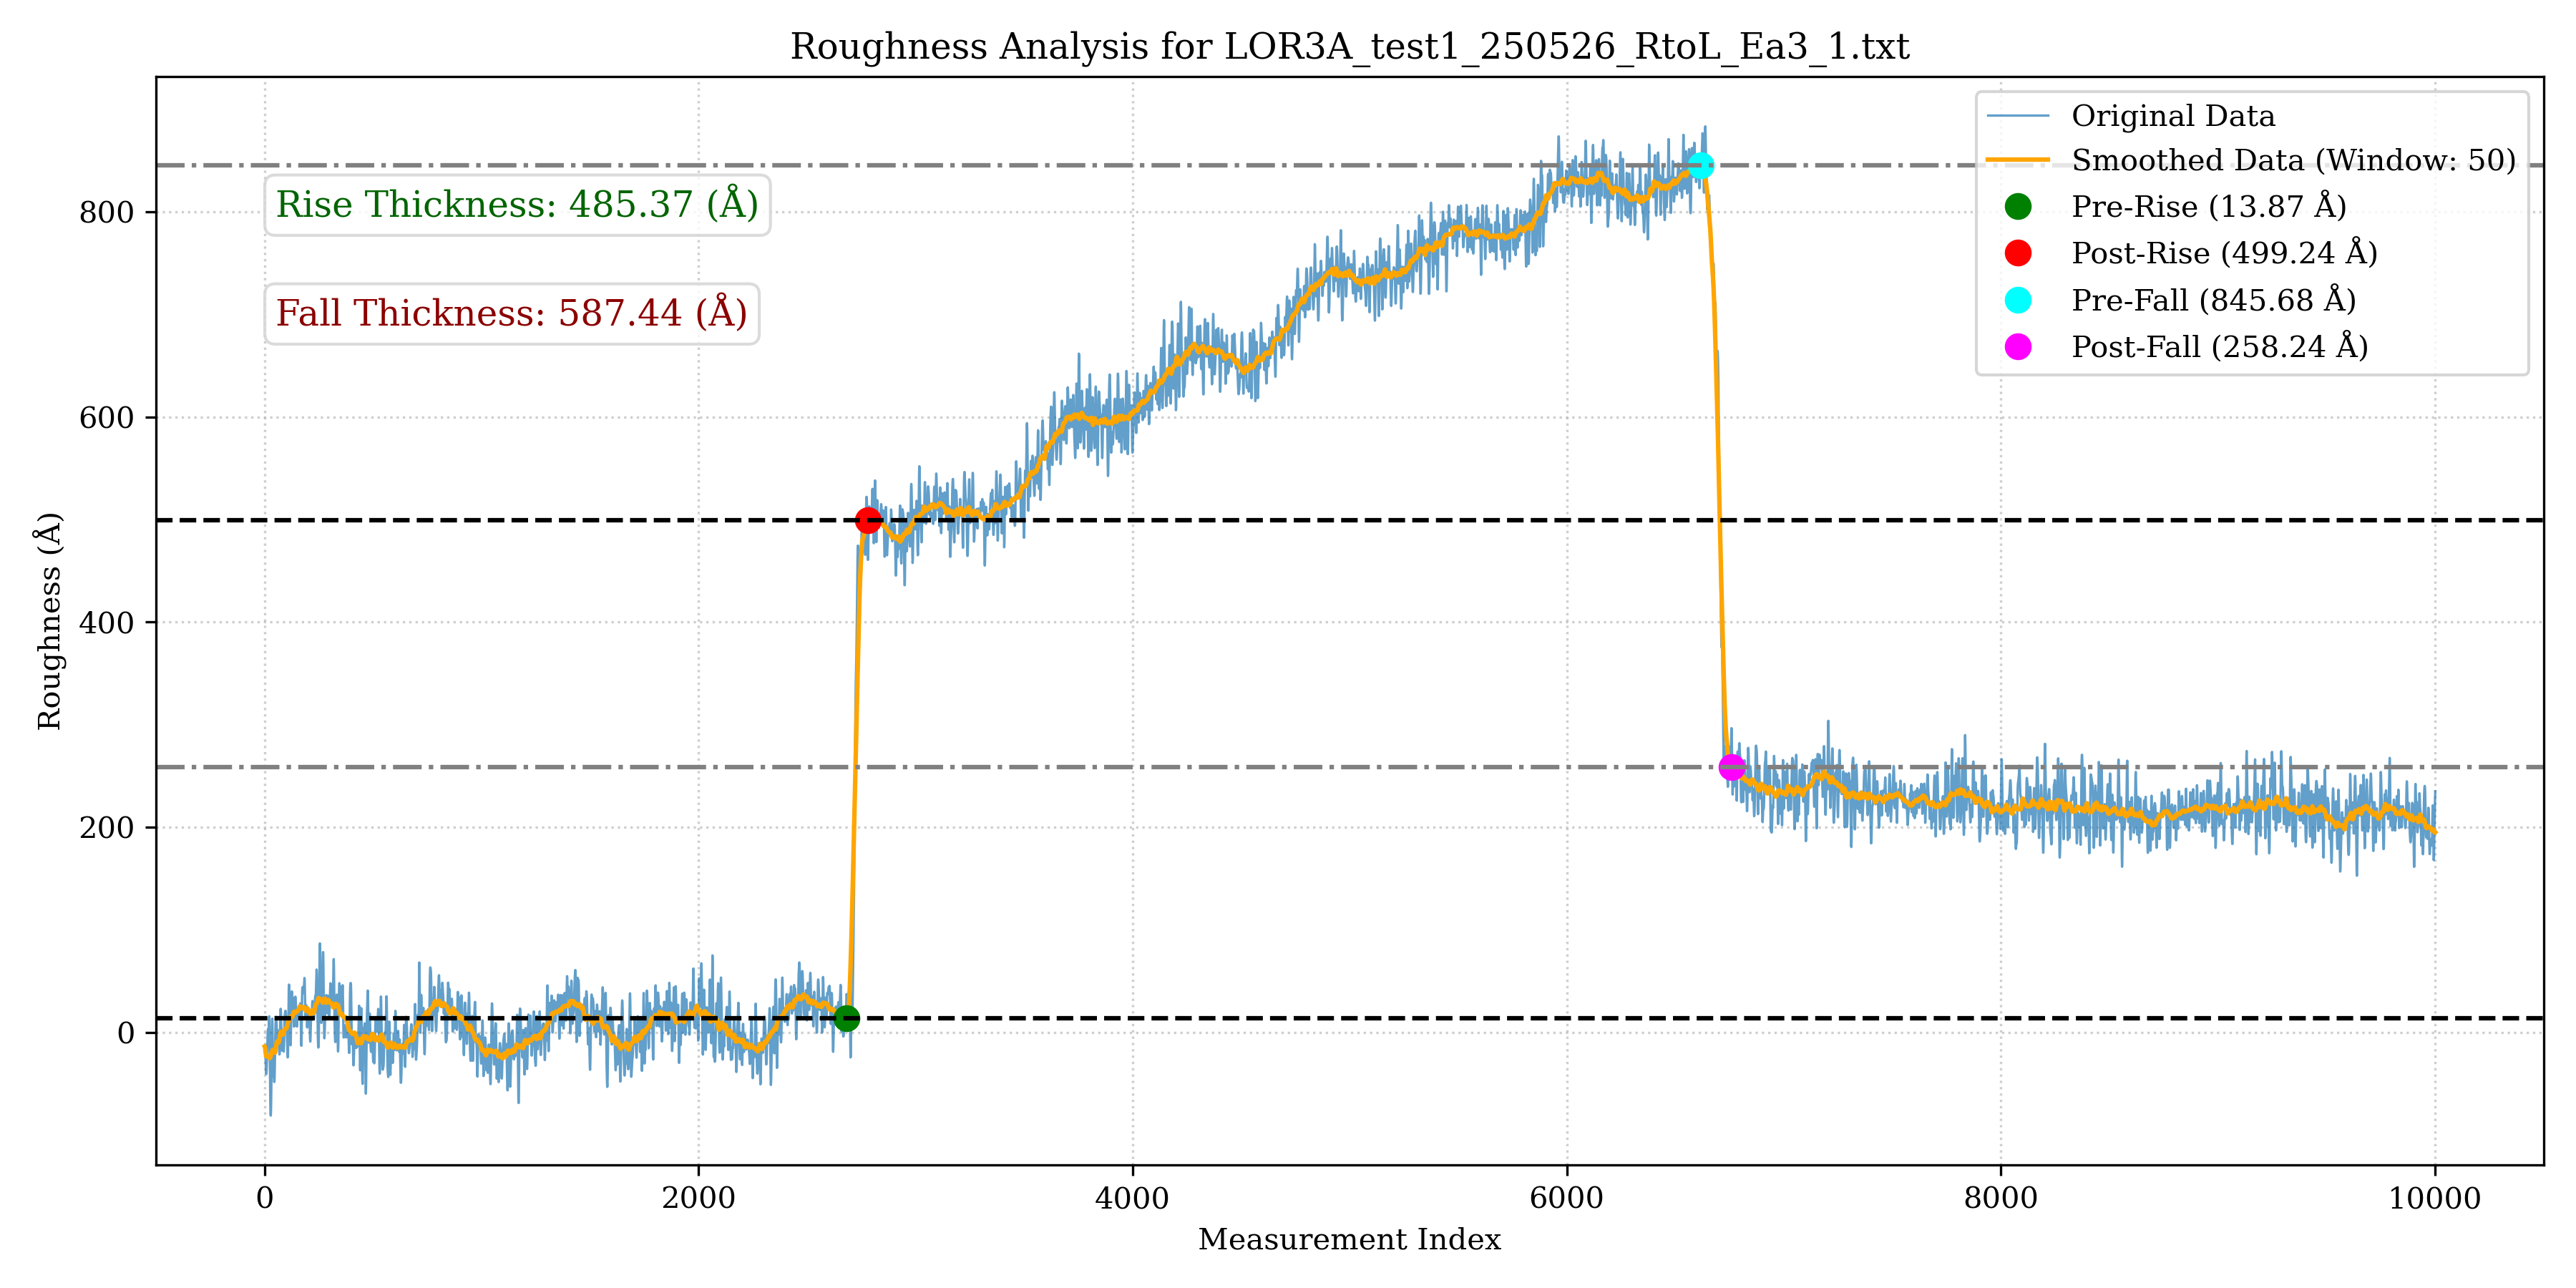
\includegraphics[width=\textwidth]{LOR3A_test1_250526_RtoL_Ea3_1.png}
    \label{fig:LOR3Atest1250526RtoLEa31}
\end{figure}
\begin{figure}[H]
    \centering
    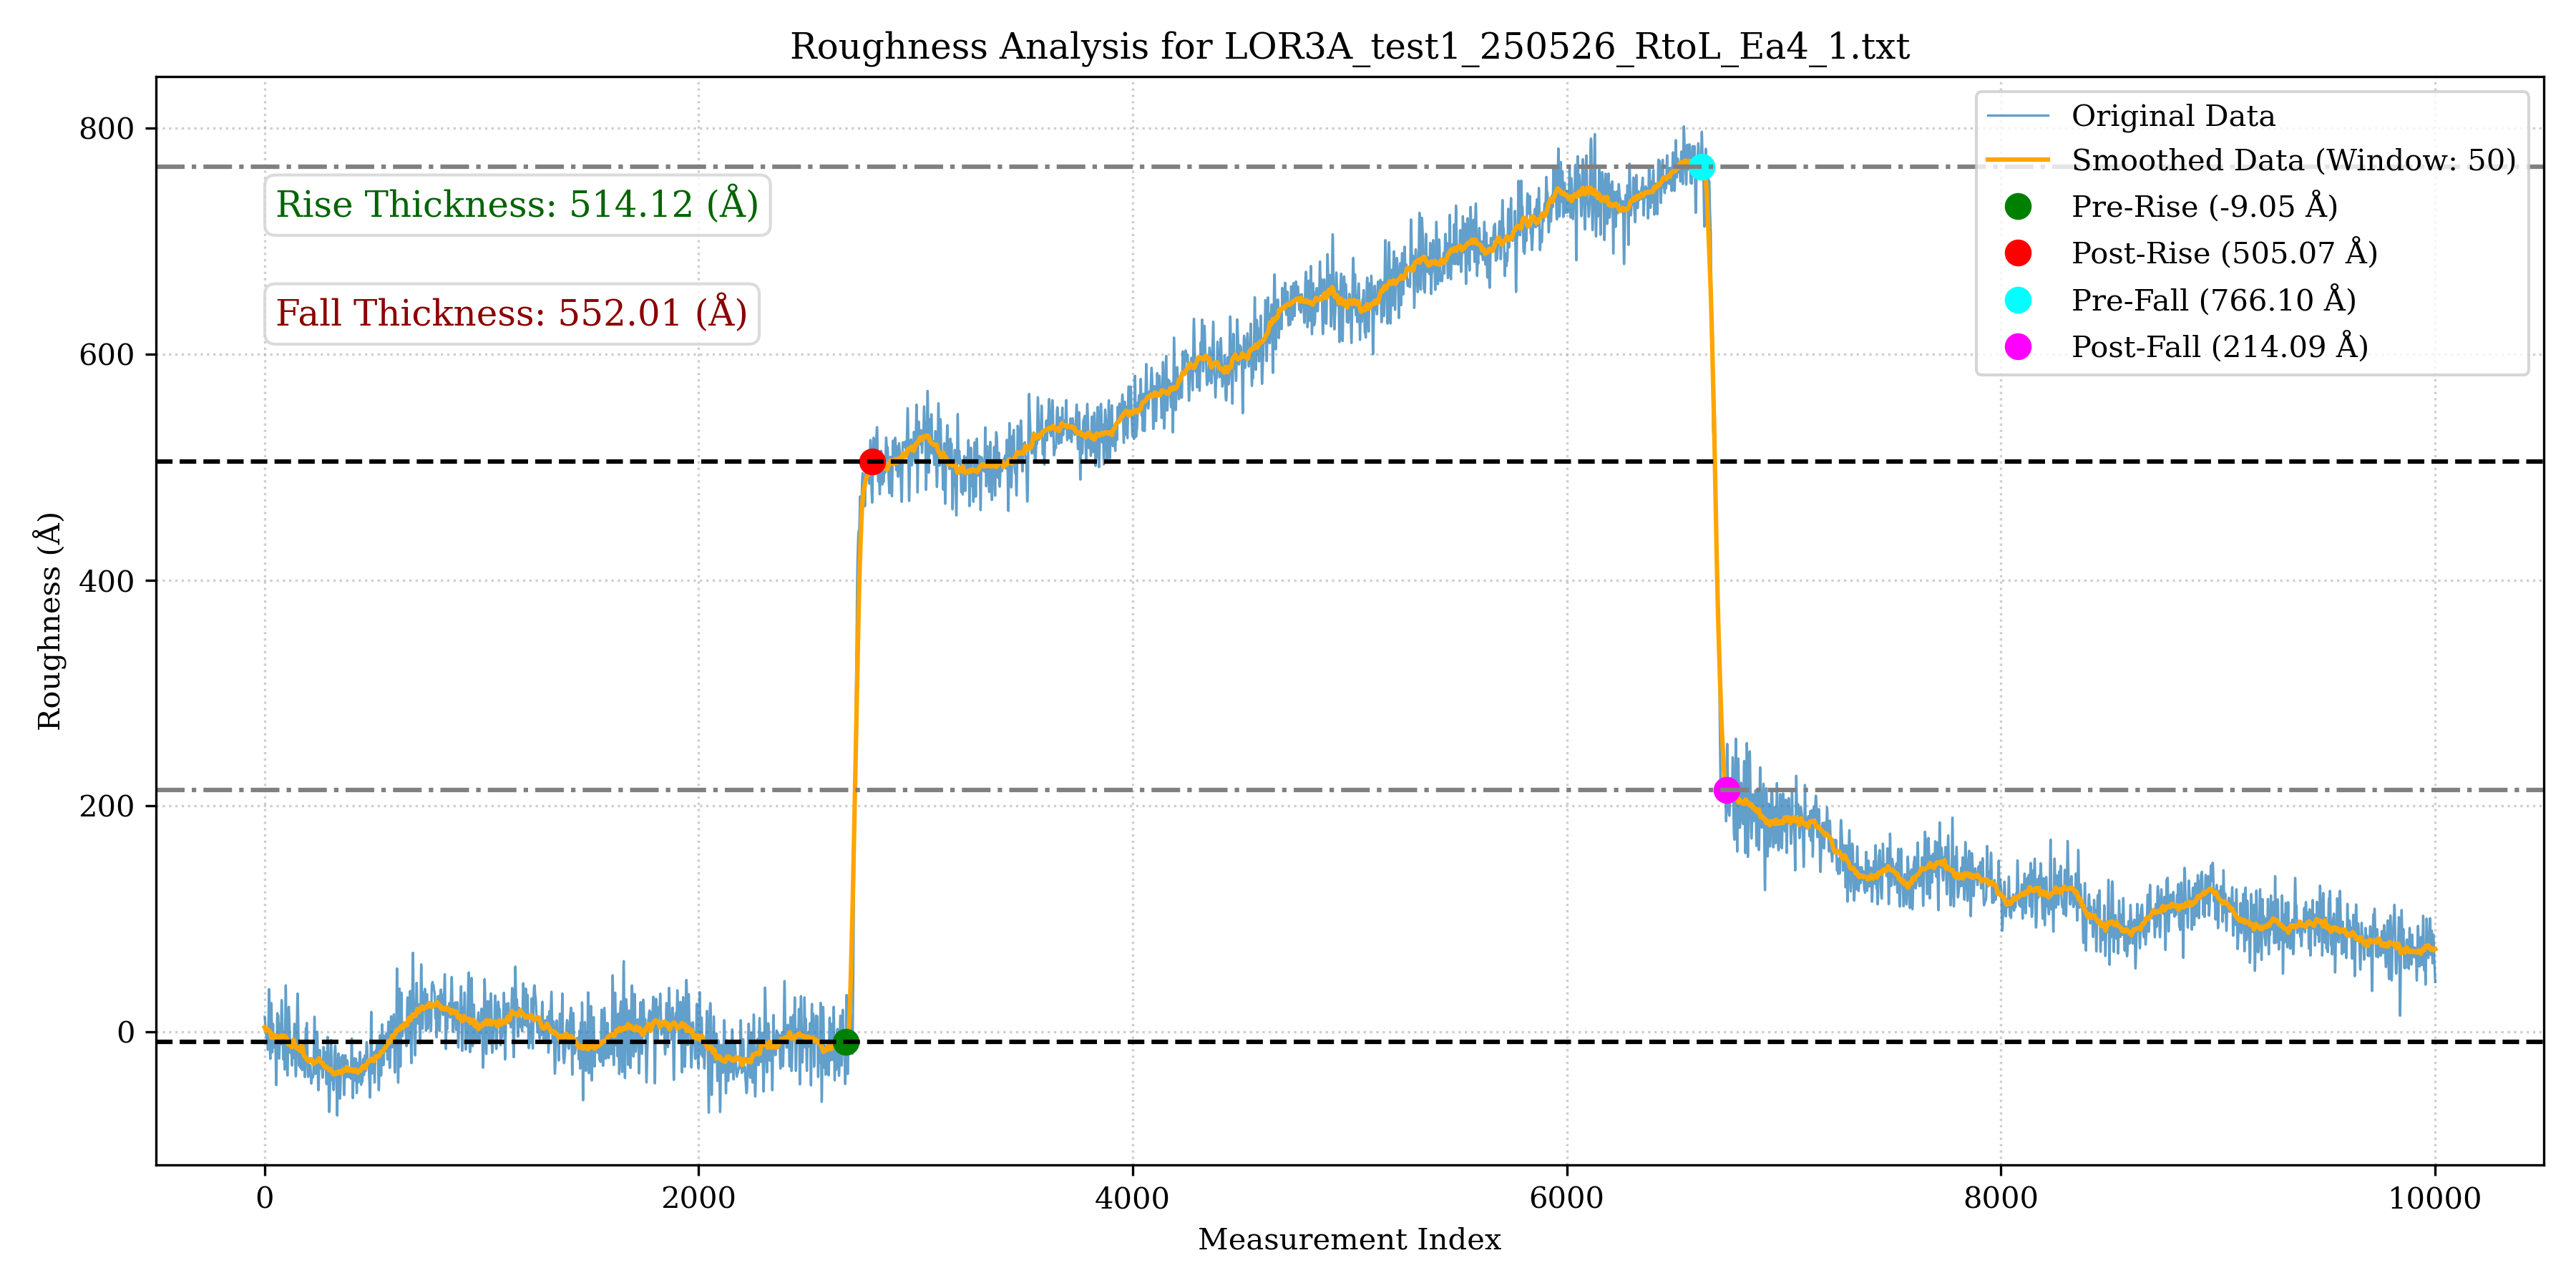
\includegraphics[width=\textwidth]{LOR3A_test1_250526_RtoL_Ea4_1.png}
    \label{fig:LOR3Atest1250526RtoLEa41}
\end{figure}
\begin{figure}[H]
    \centering
    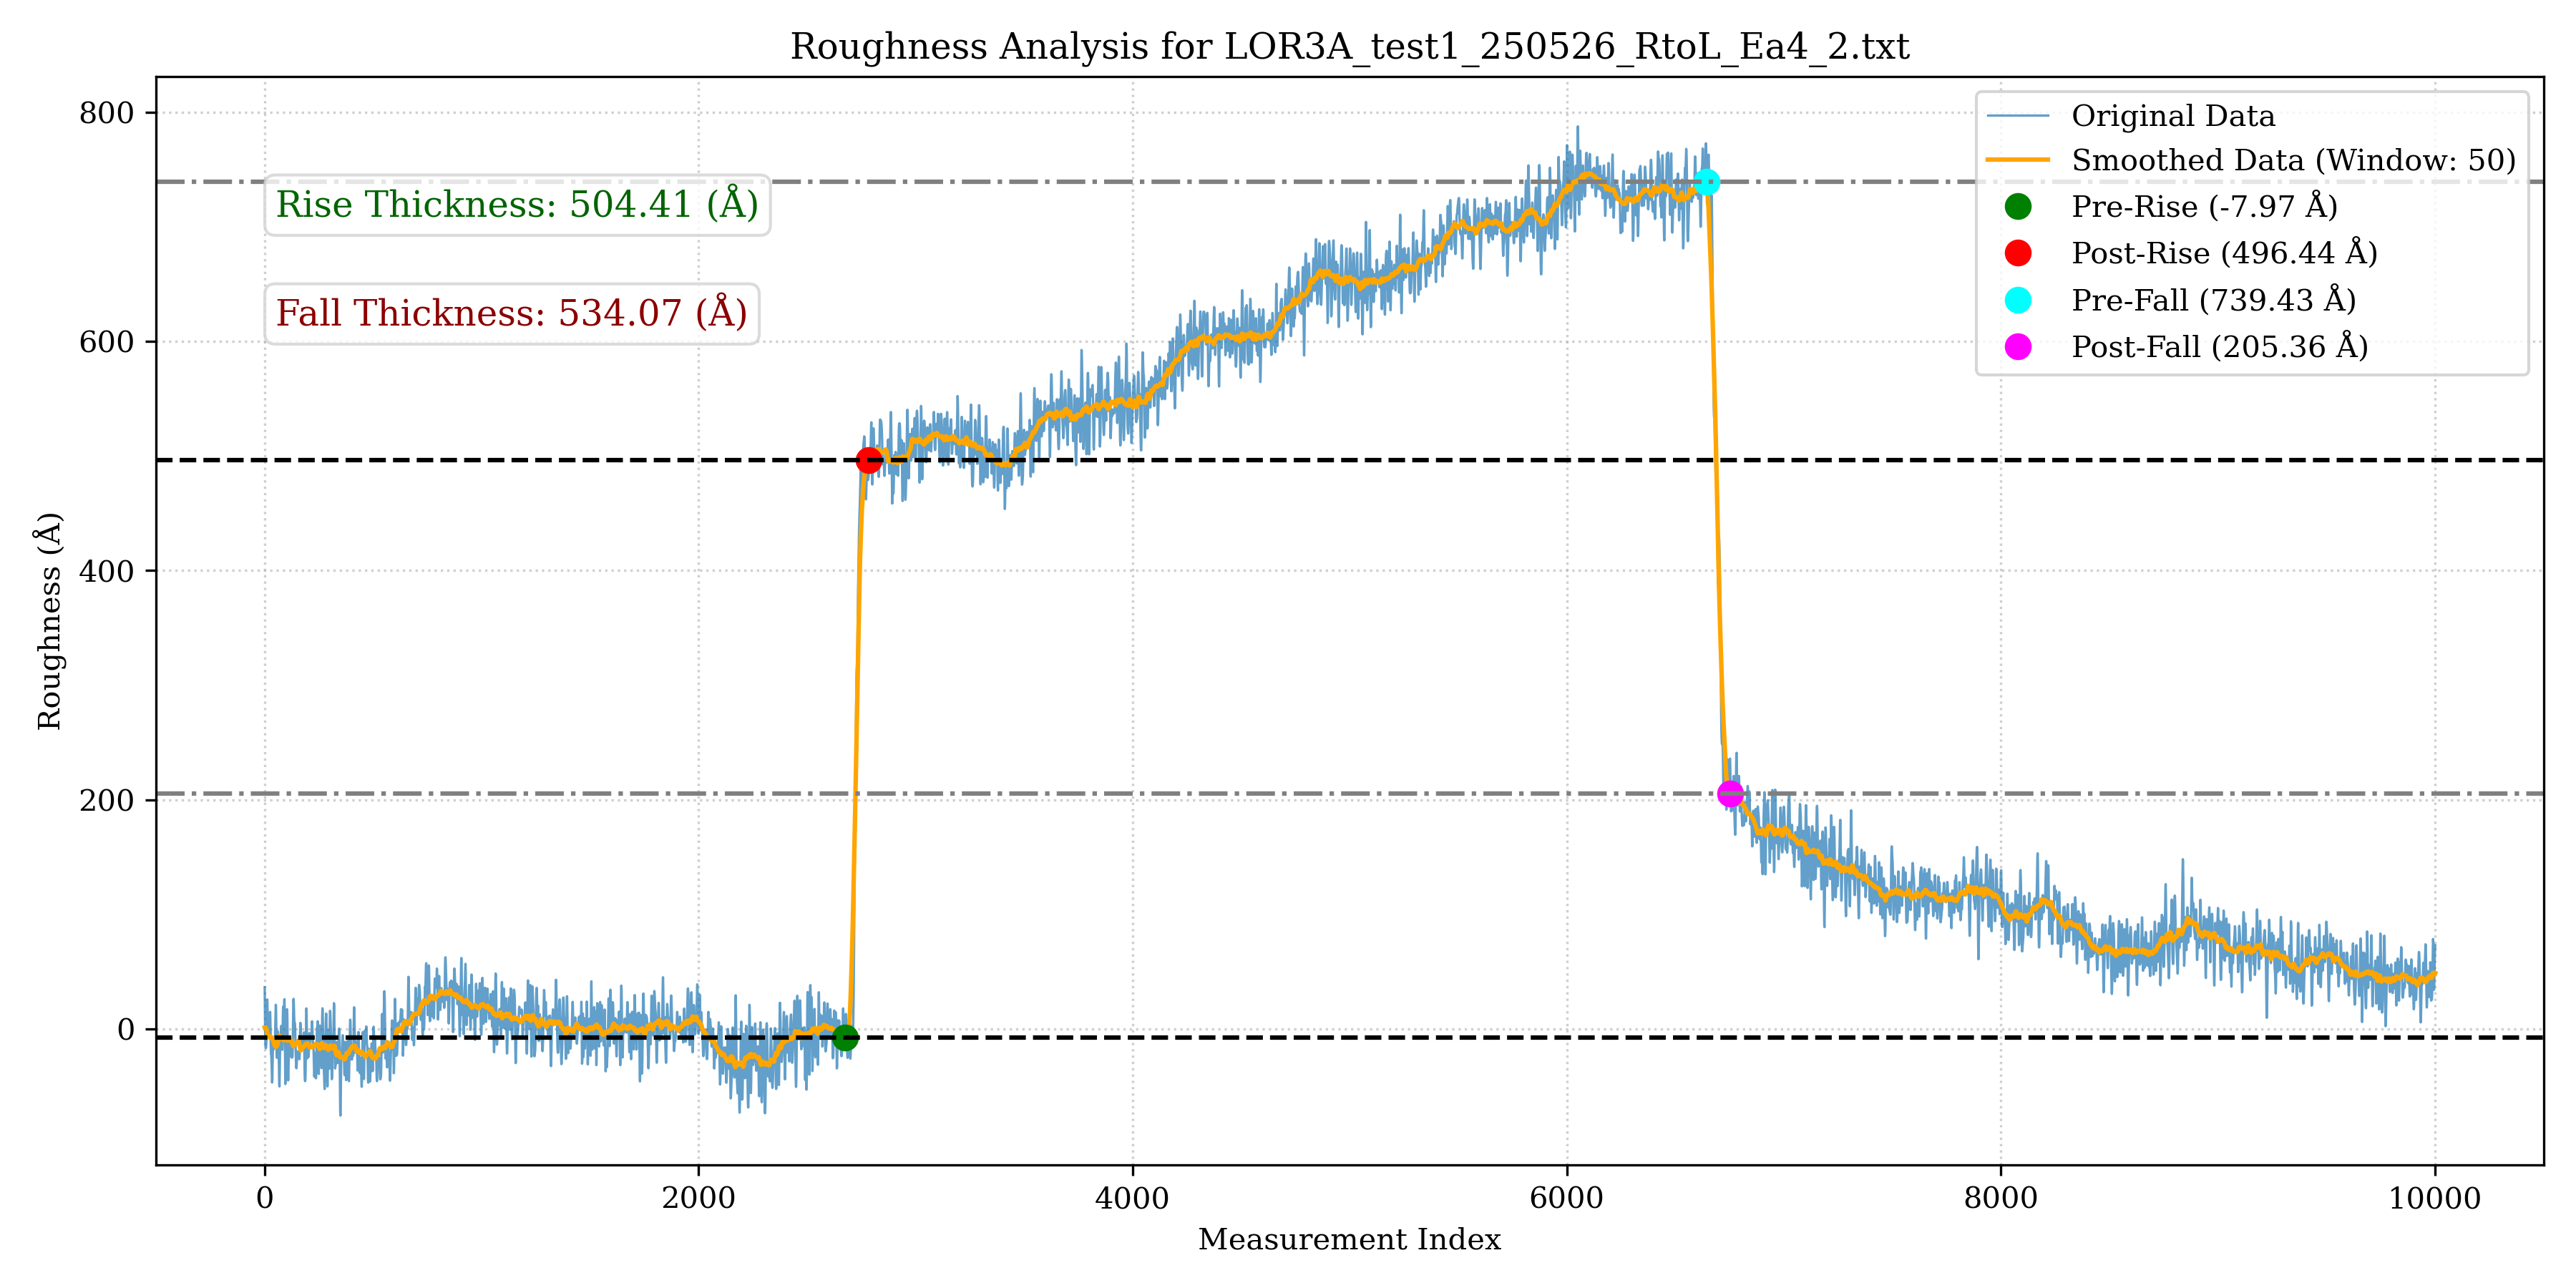
\includegraphics[width=\textwidth]{LOR3A_test1_250526_RtoL_Ea4_2.png}
    \label{fig:LOR3Atest1250526RtoLEa42}
\end{figure}
\begin{figure}[H]
    \centering
    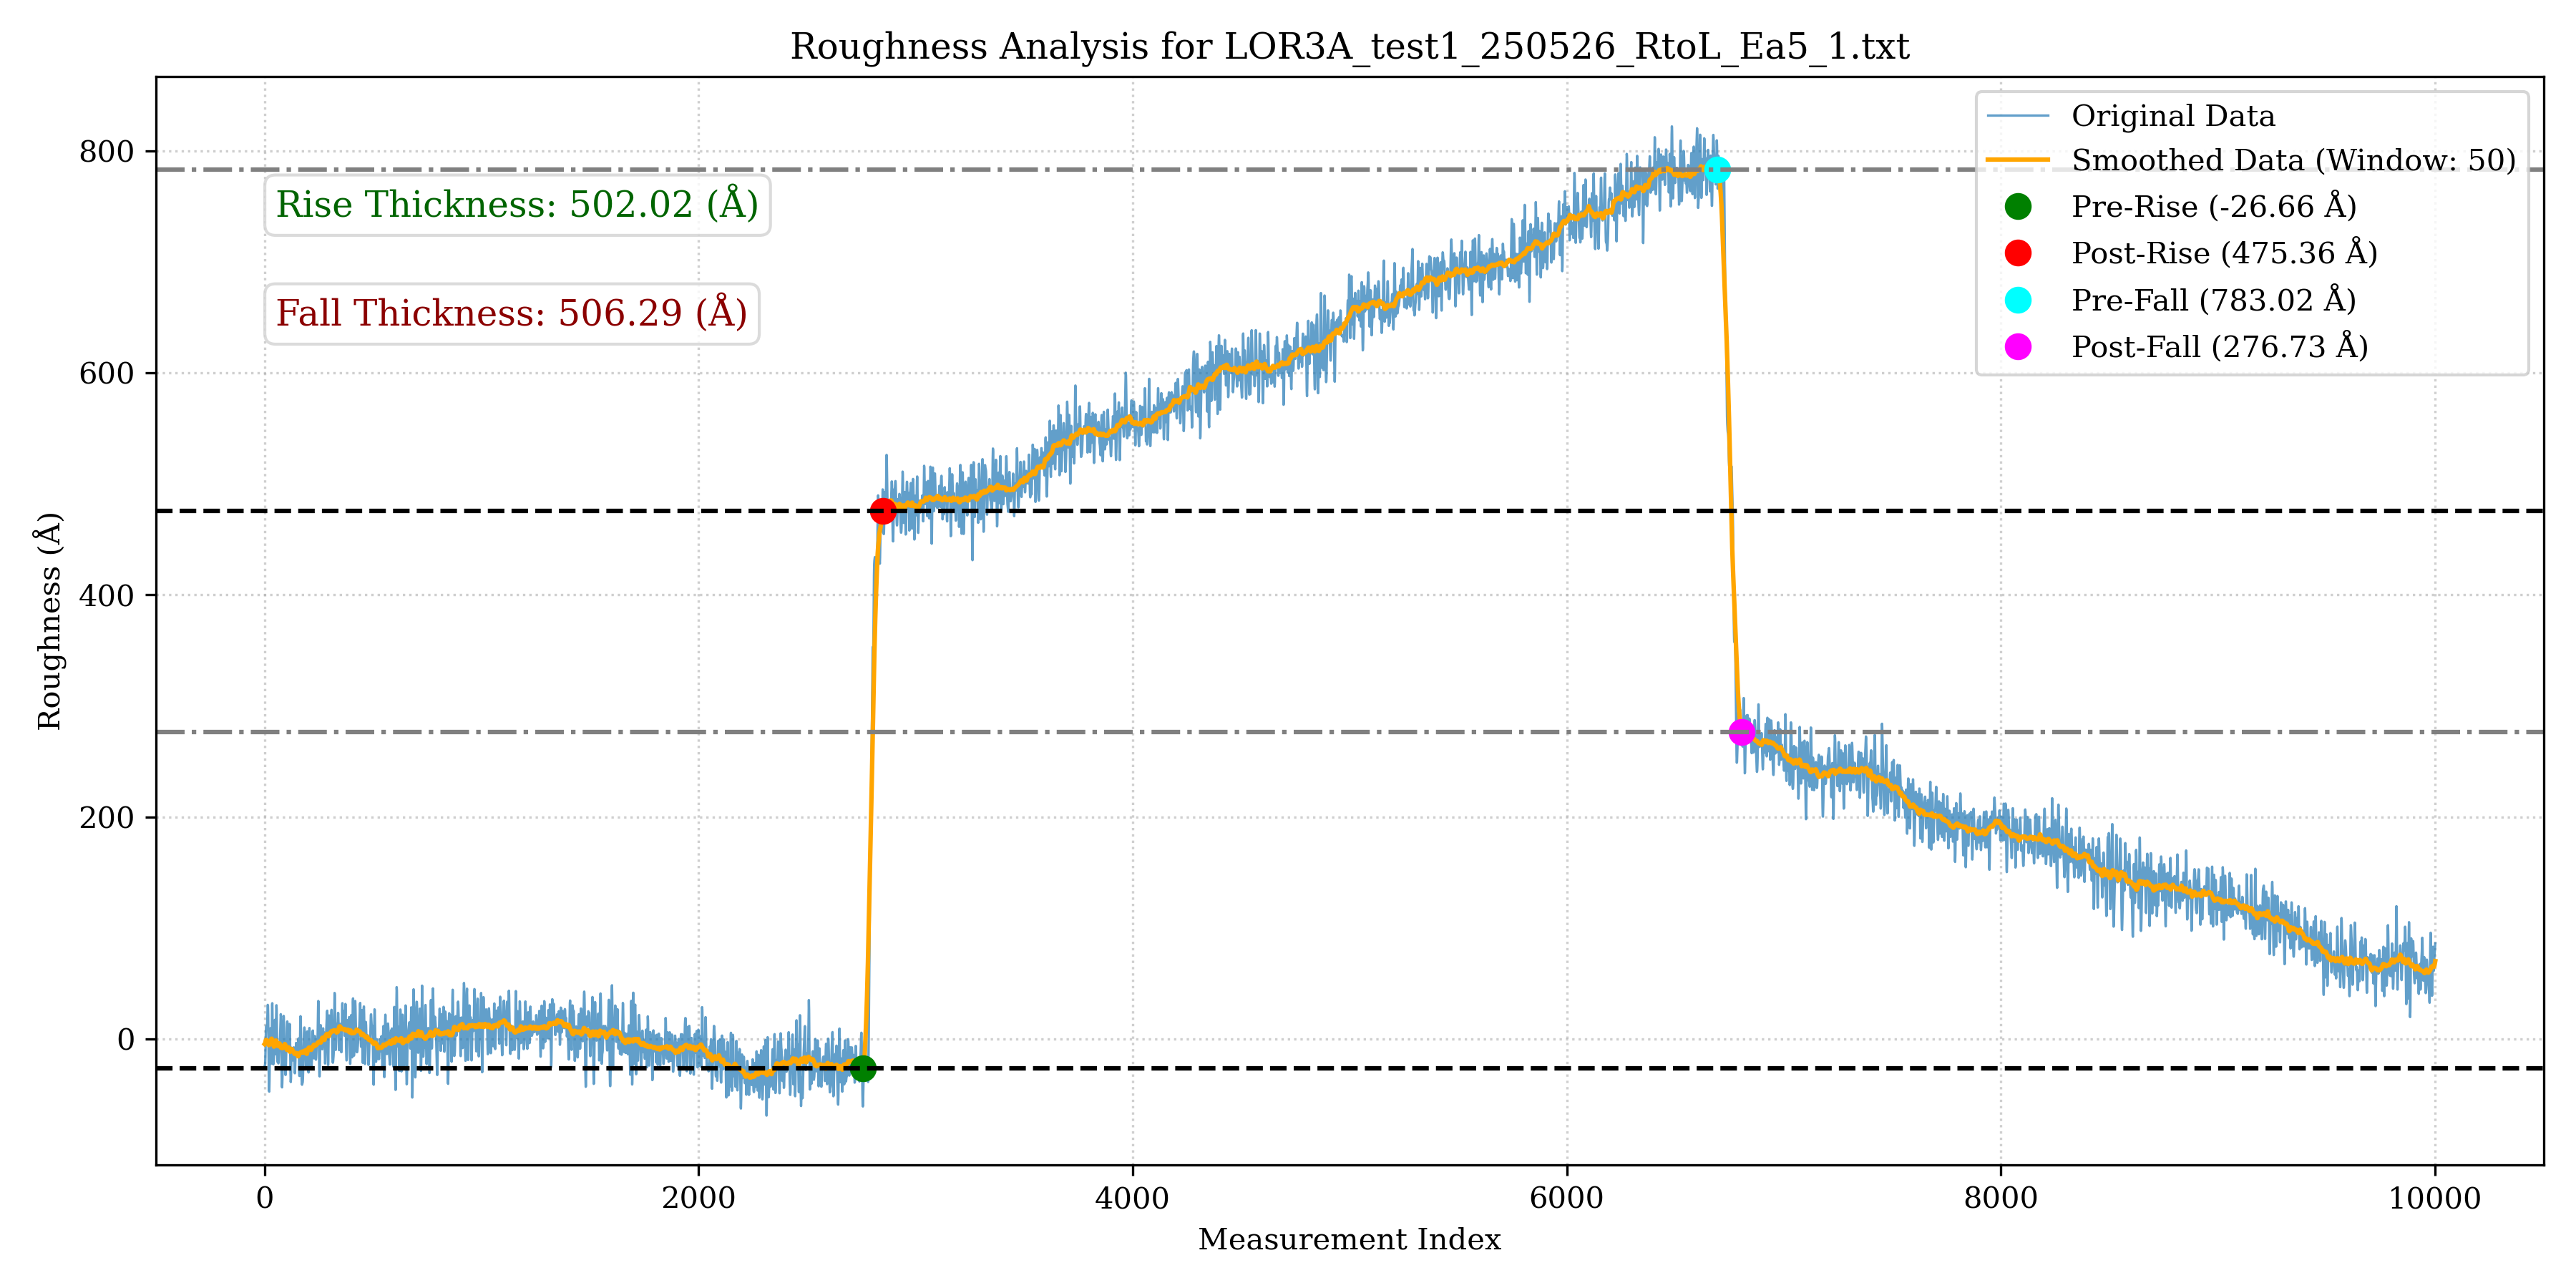
\includegraphics[width=\textwidth]{LOR3A_test1_250526_RtoL_Ea5_1.png}
    \label{fig:LOR3Atest1250526RtoLEa51}
\end{figure}
\begin{figure}[H]
    \centering
    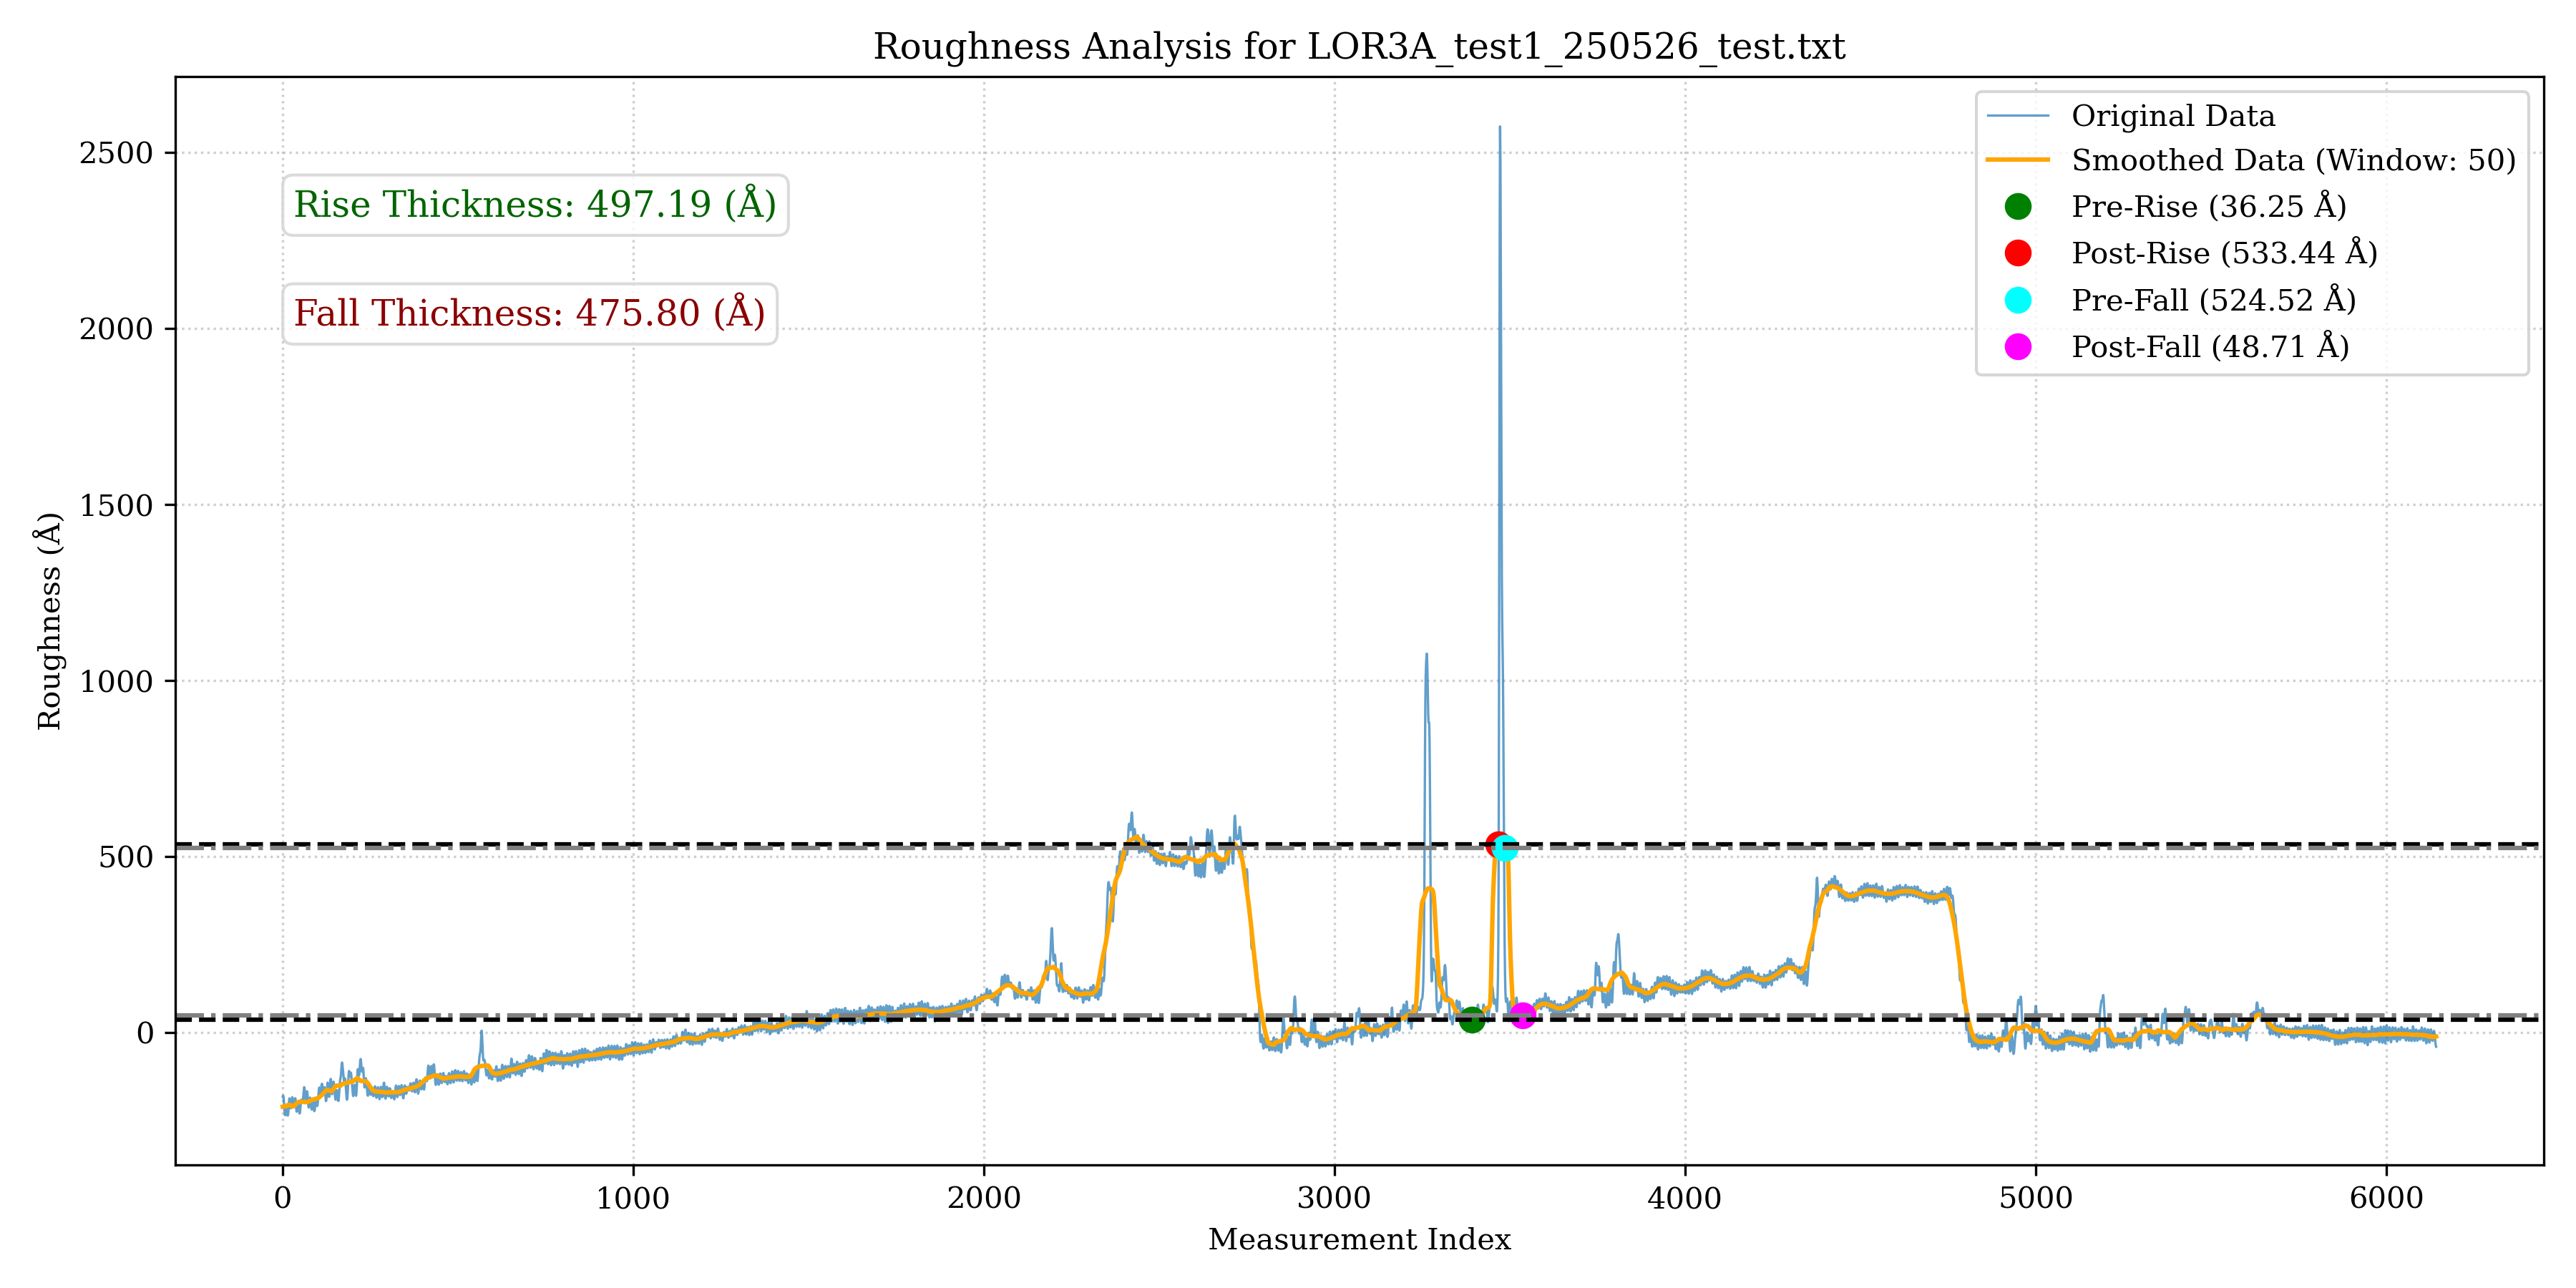
\includegraphics[width=\textwidth]{LOR3A_test1_250526_test.png}
    \label{fig:LOR3Atest1250526test}
\end{figure}
\begin{figure}[H]
    \centering
    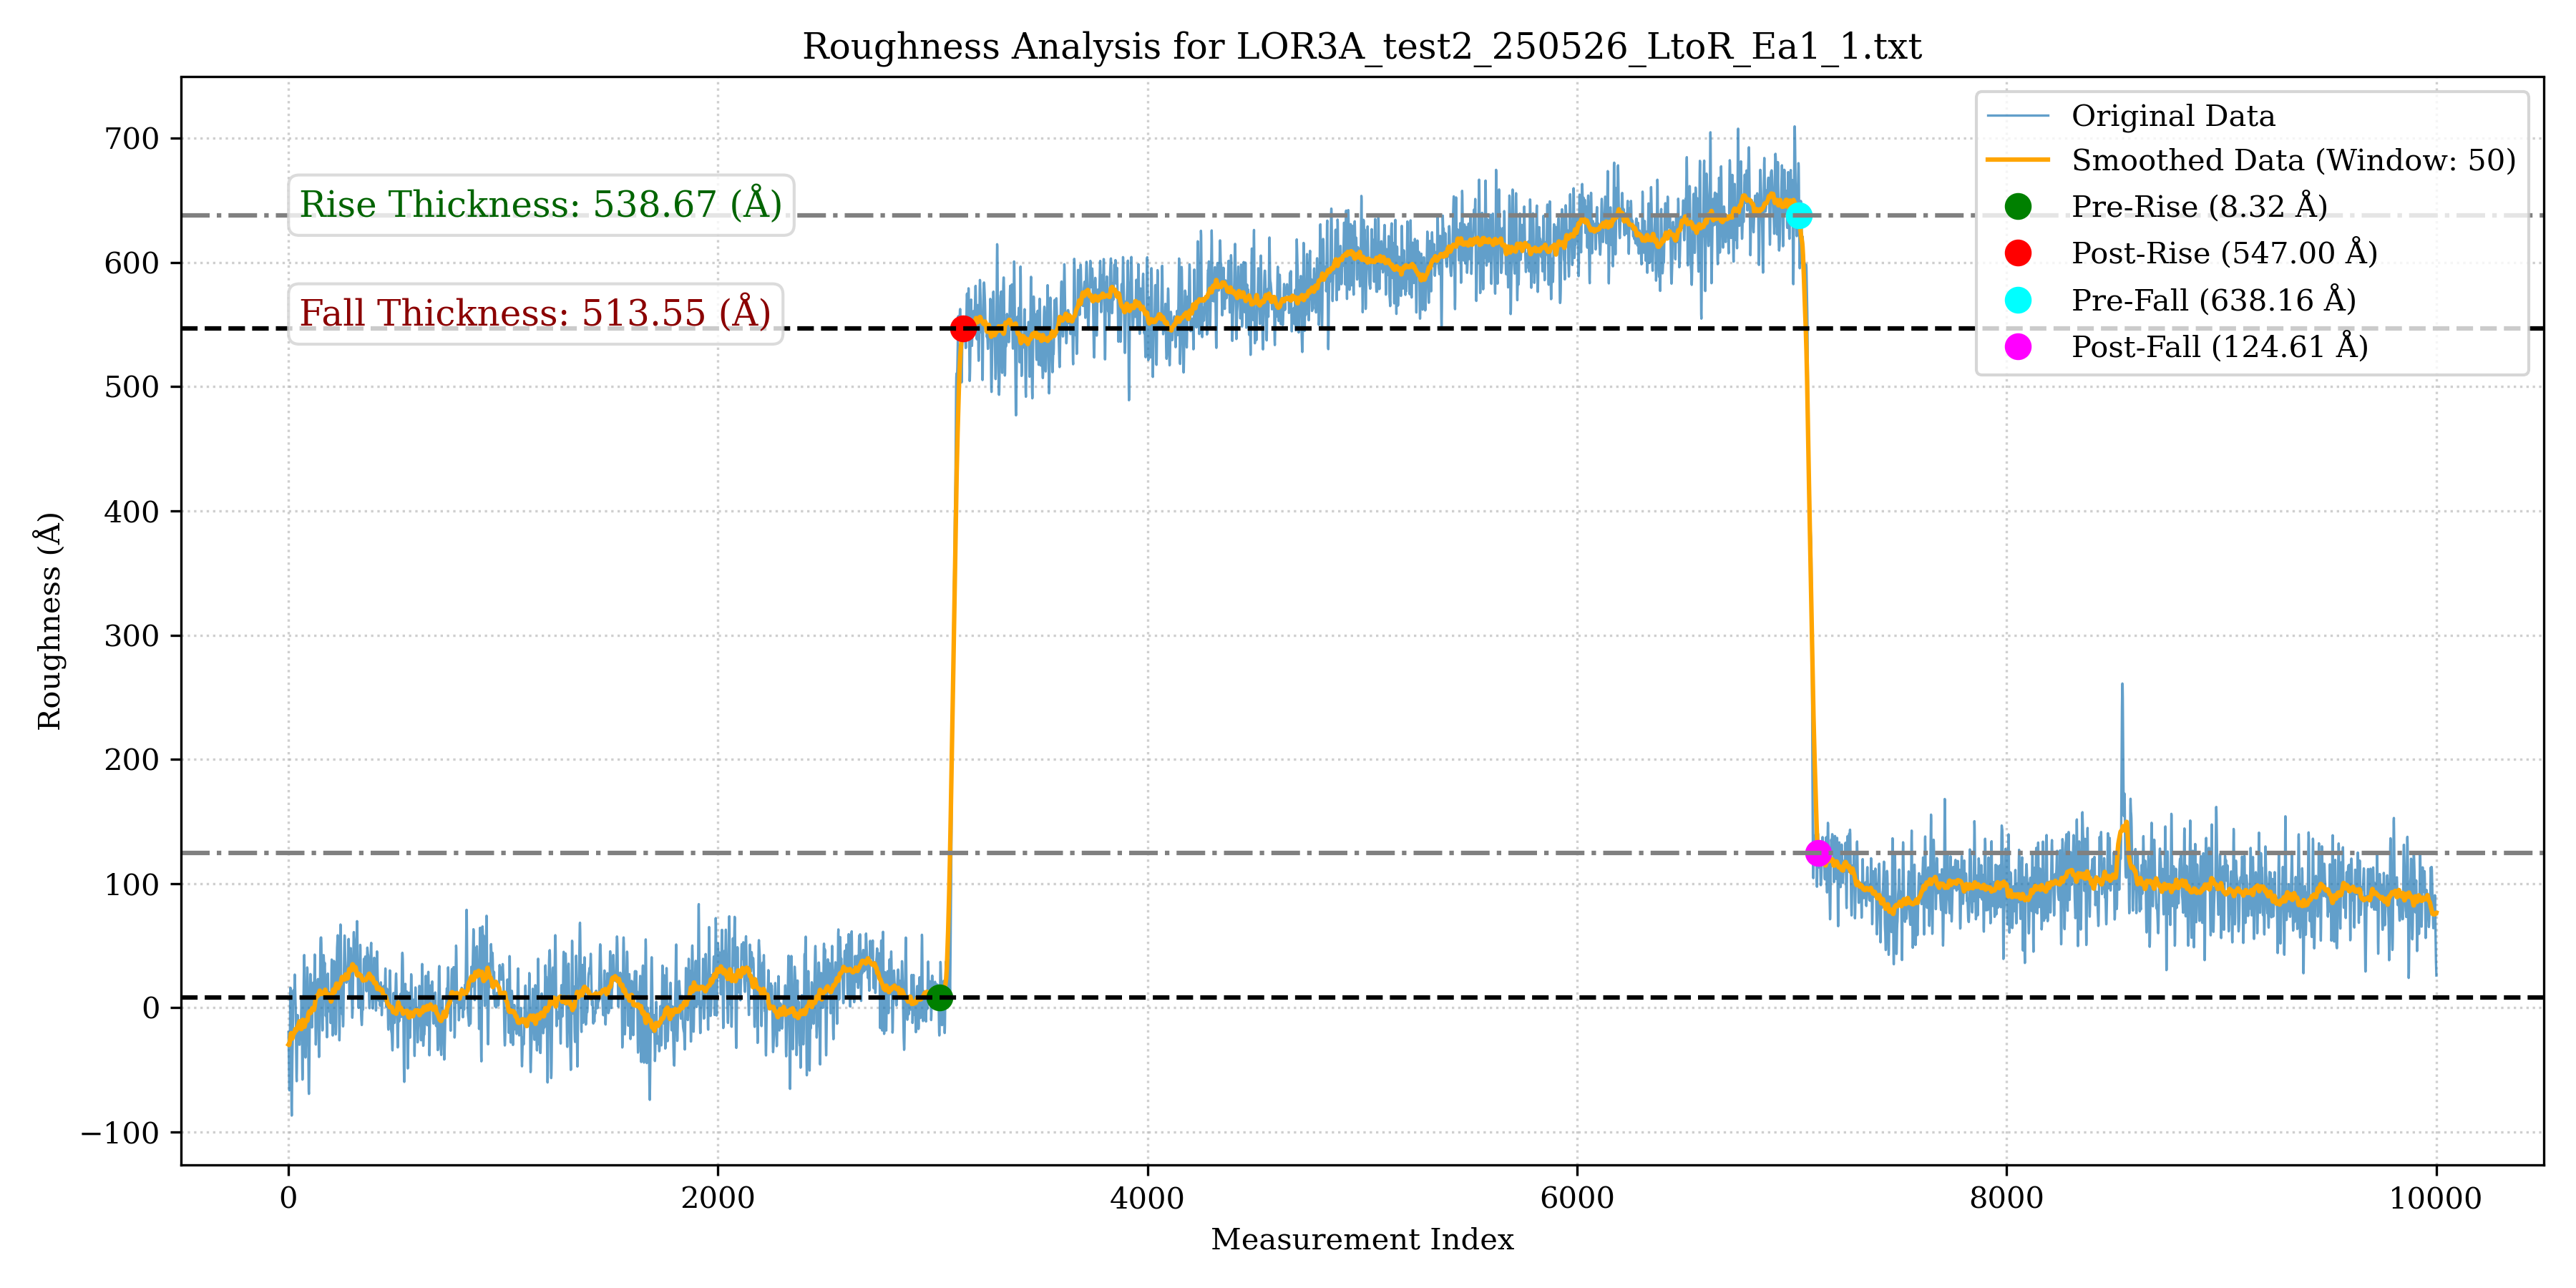
\includegraphics[width=\textwidth]{LOR3A_test2_250526_LtoR_Ea1_1.png}
    \label{fig:LOR3Atest2250526LtoREa11}
\end{figure}
\begin{figure}[H]
    \centering
    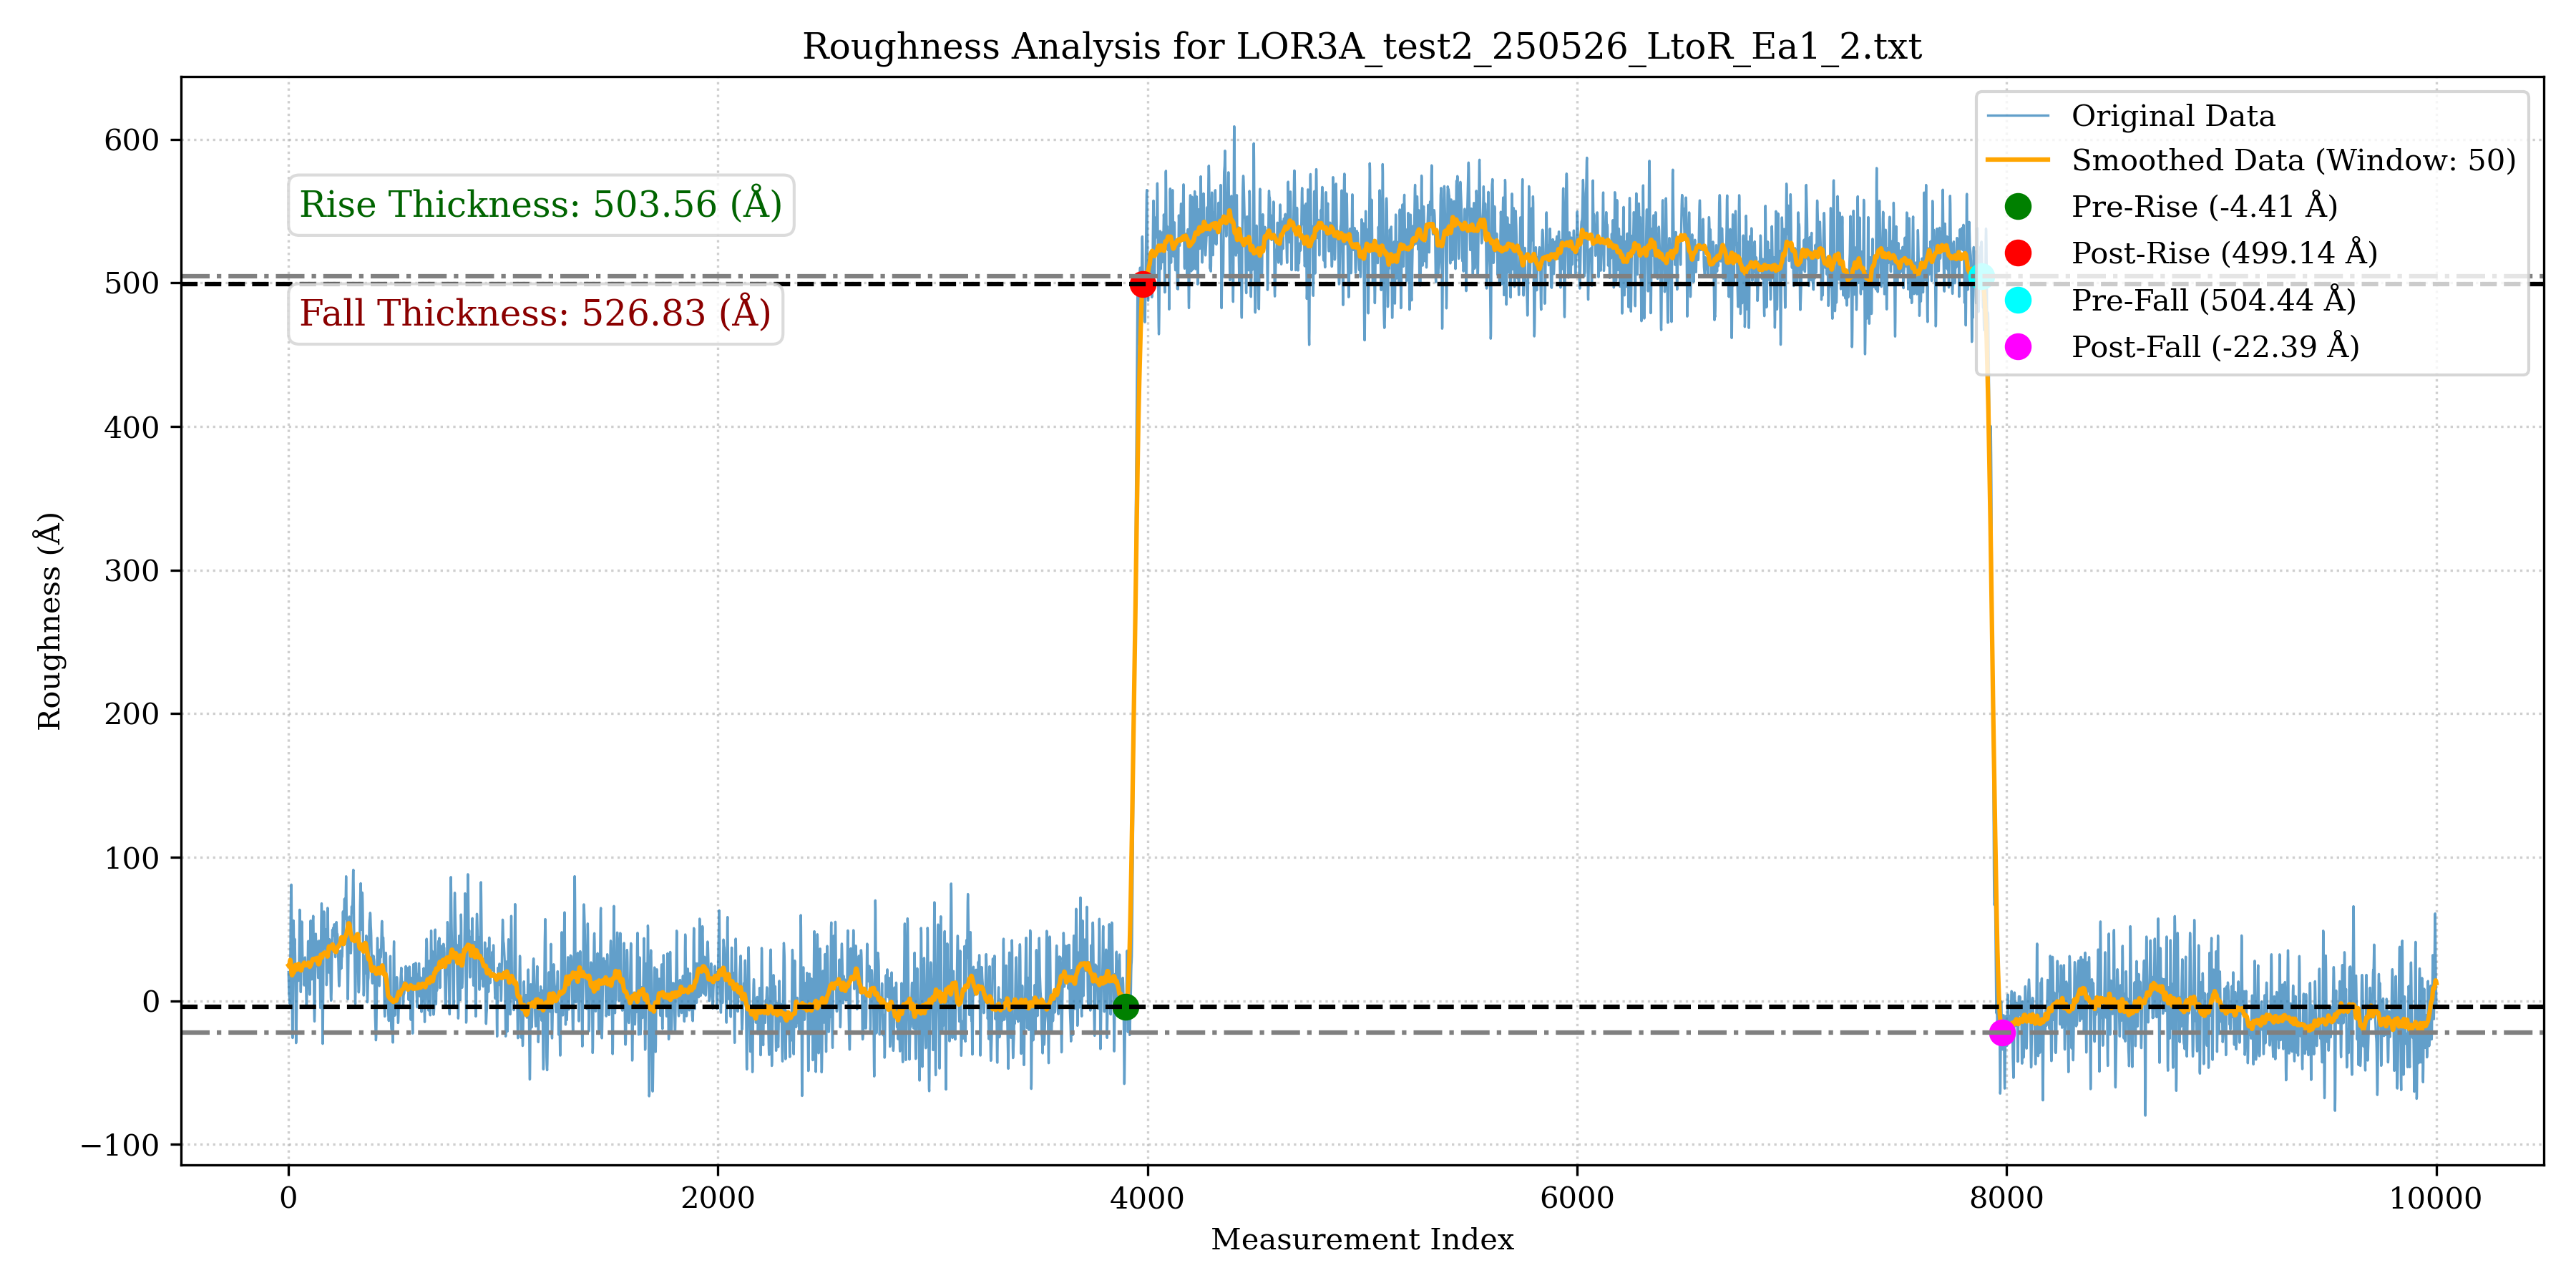
\includegraphics[width=\textwidth]{LOR3A_test2_250526_LtoR_Ea1_2.png}
    \label{fig:LOR3Atest2250526LtoREa12}
\end{figure}
\begin{figure}[H]
    \centering
    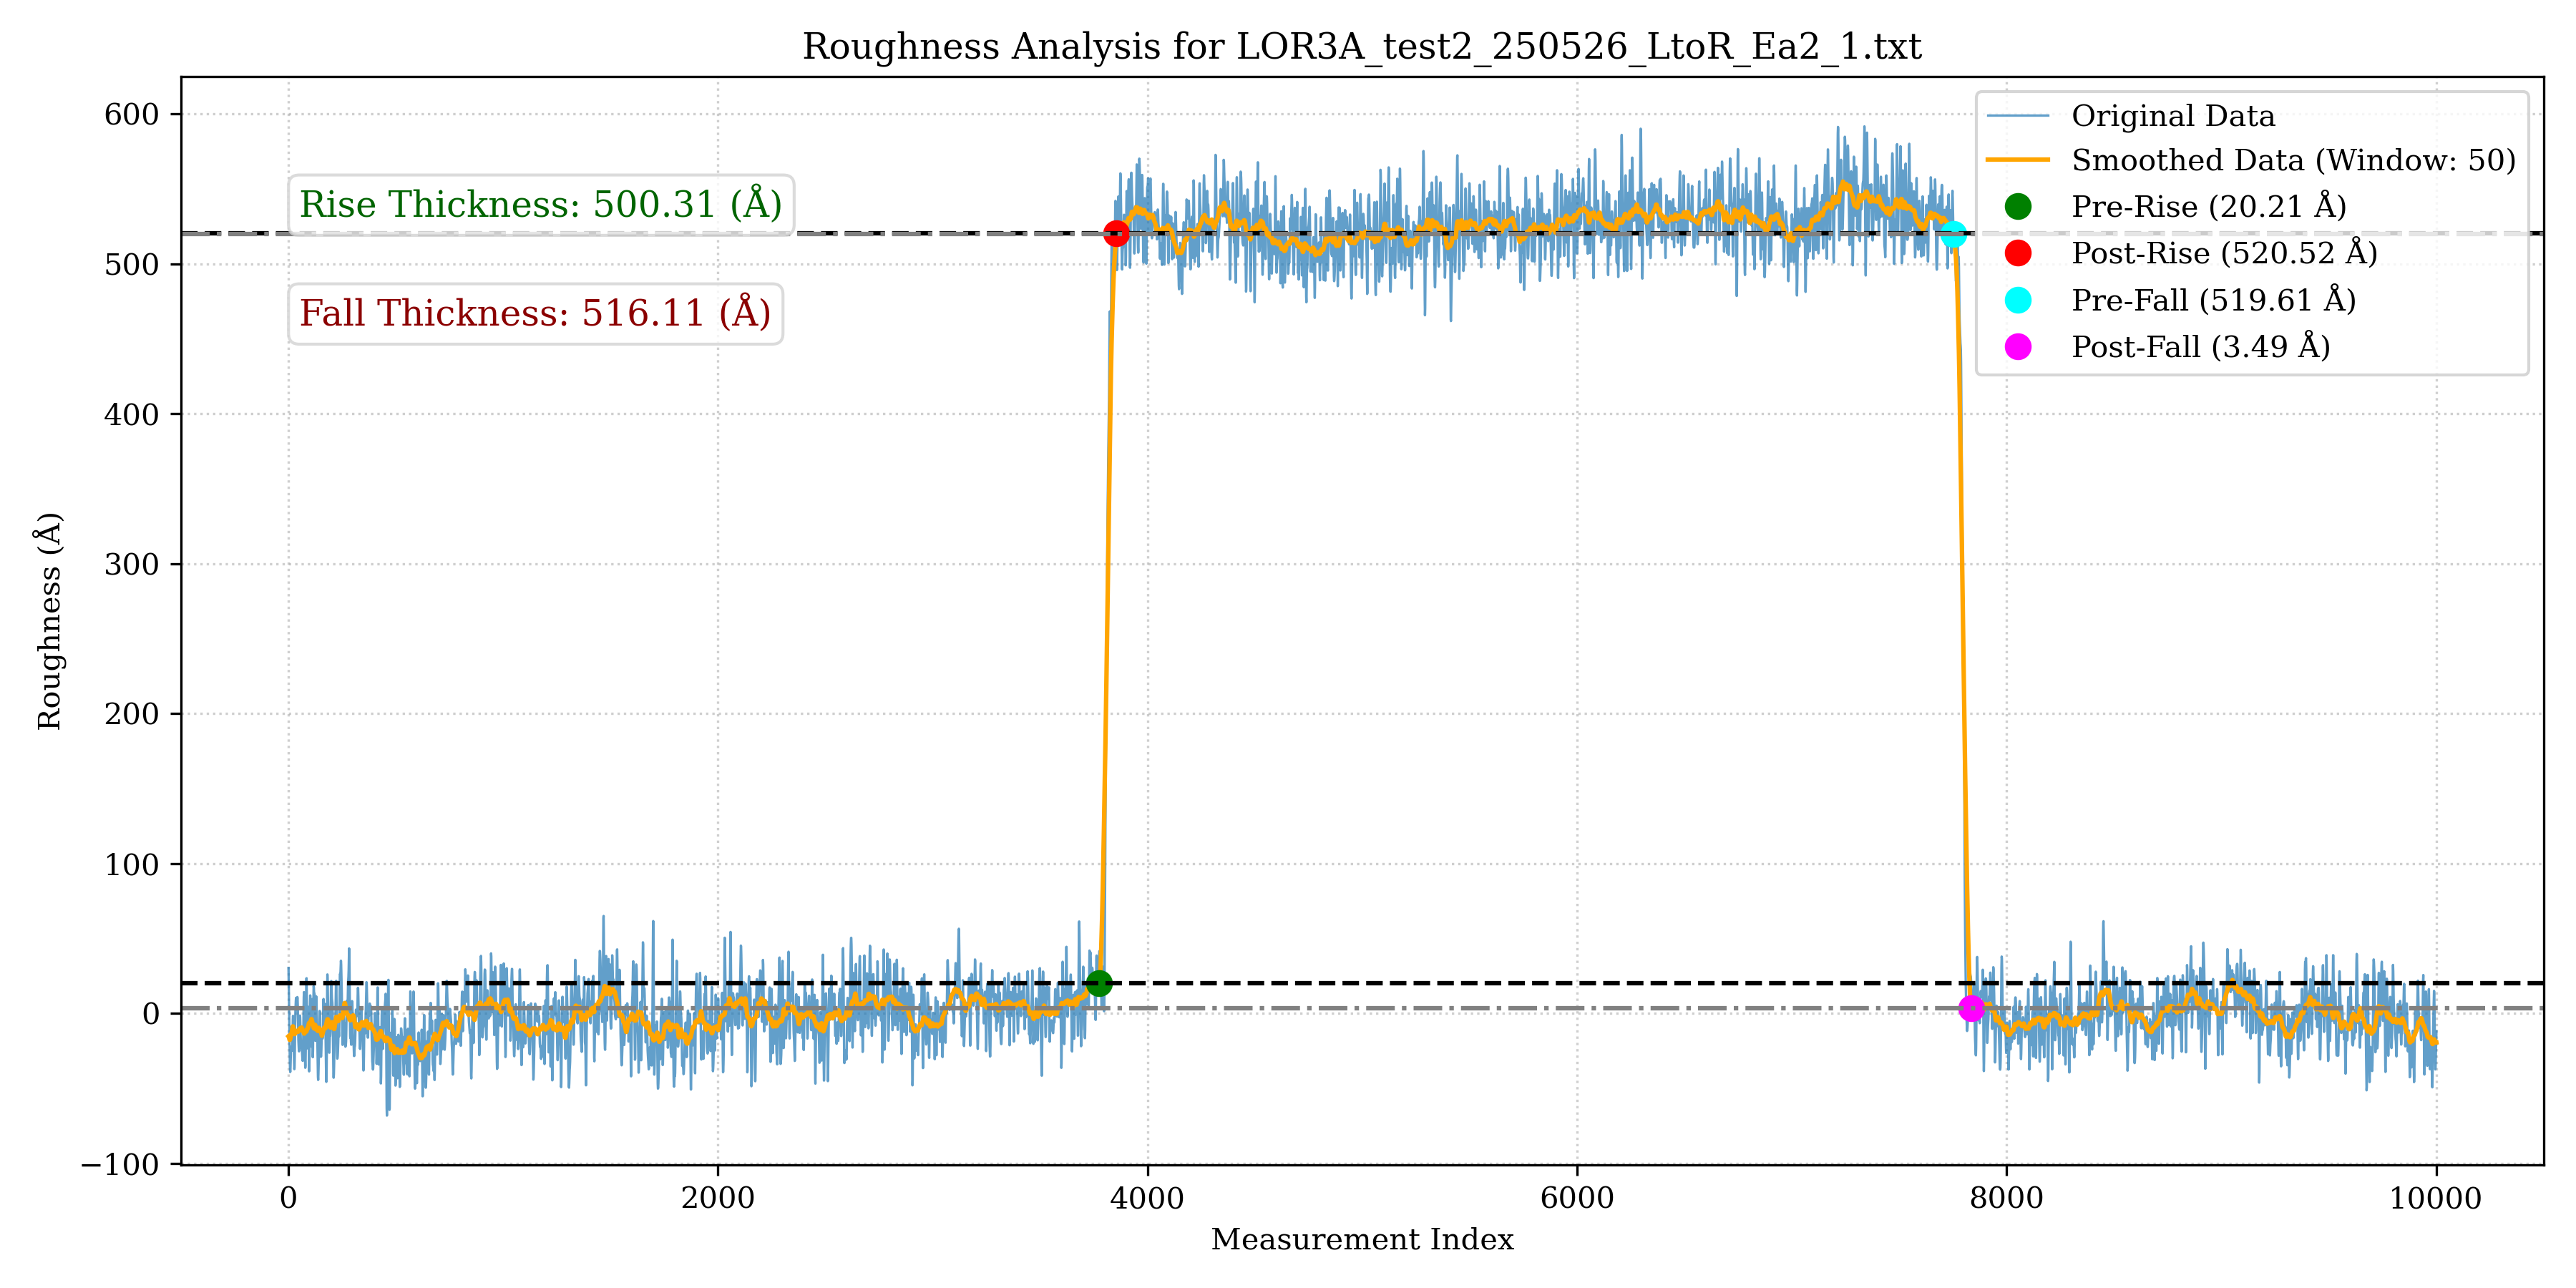
\includegraphics[width=\textwidth]{LOR3A_test2_250526_LtoR_Ea2_1.png}
    \label{fig:LOR3Atest2250526LtoREa21}
\end{figure}
\begin{figure}[H]
    \centering
    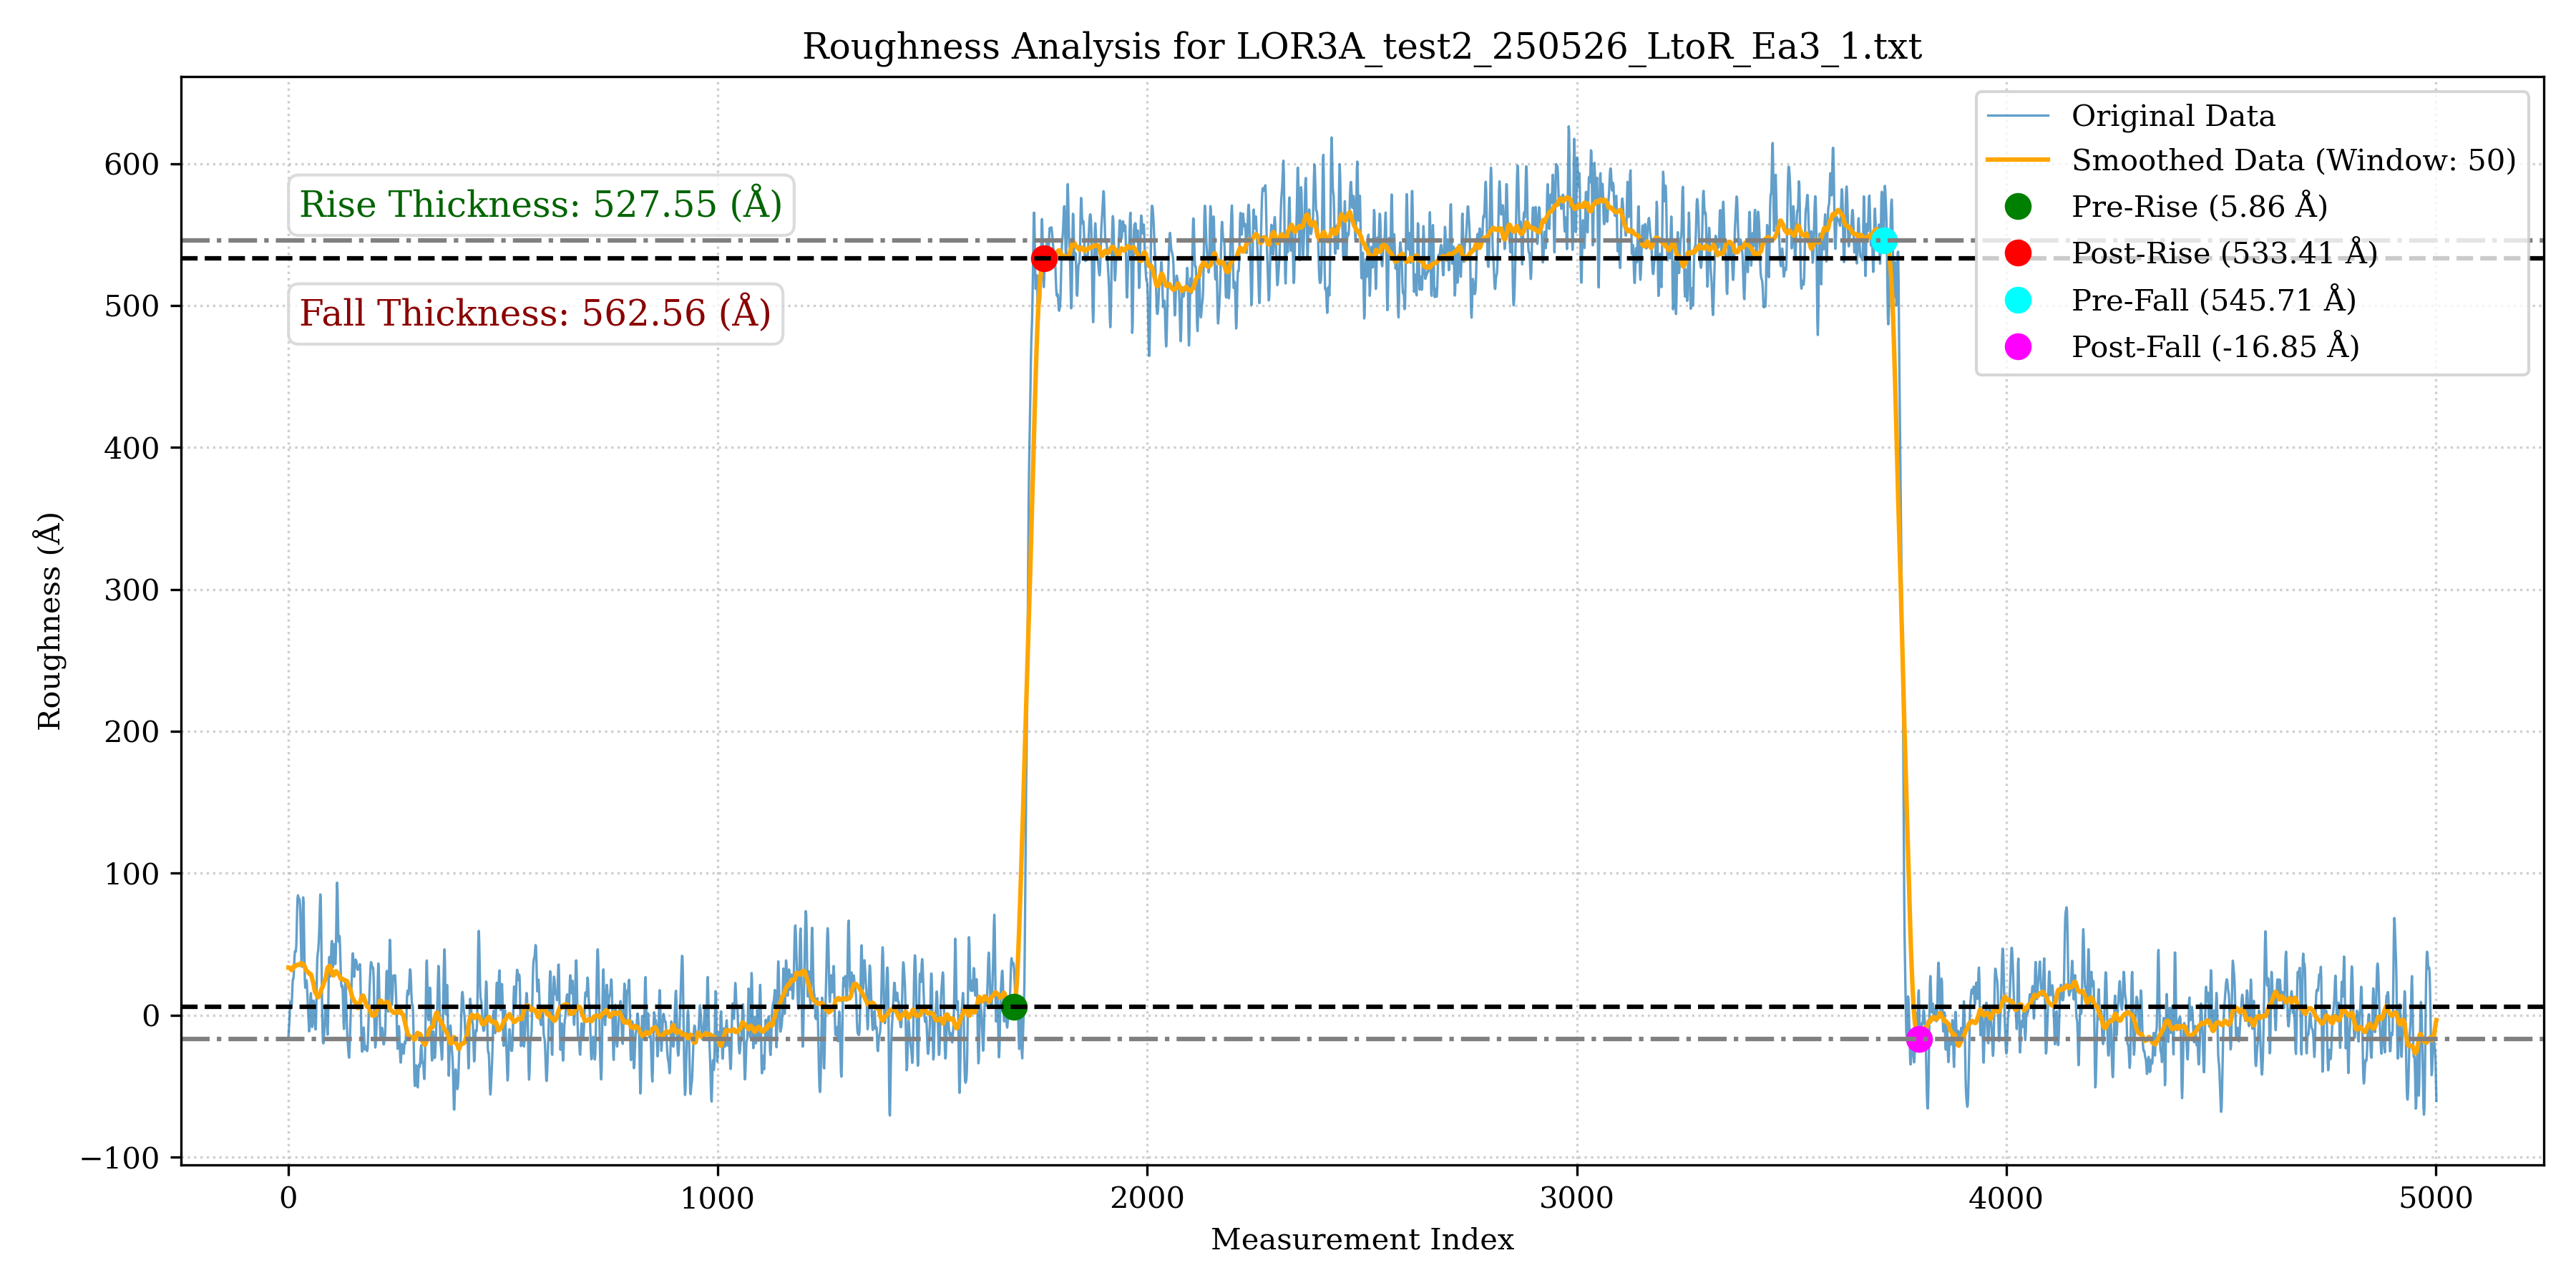
\includegraphics[width=\textwidth]{LOR3A_test2_250526_LtoR_Ea3_1.png}
    \label{fig:LOR3Atest2250526LtoREa31}
\end{figure}
\begin{figure}[H]
    \centering
    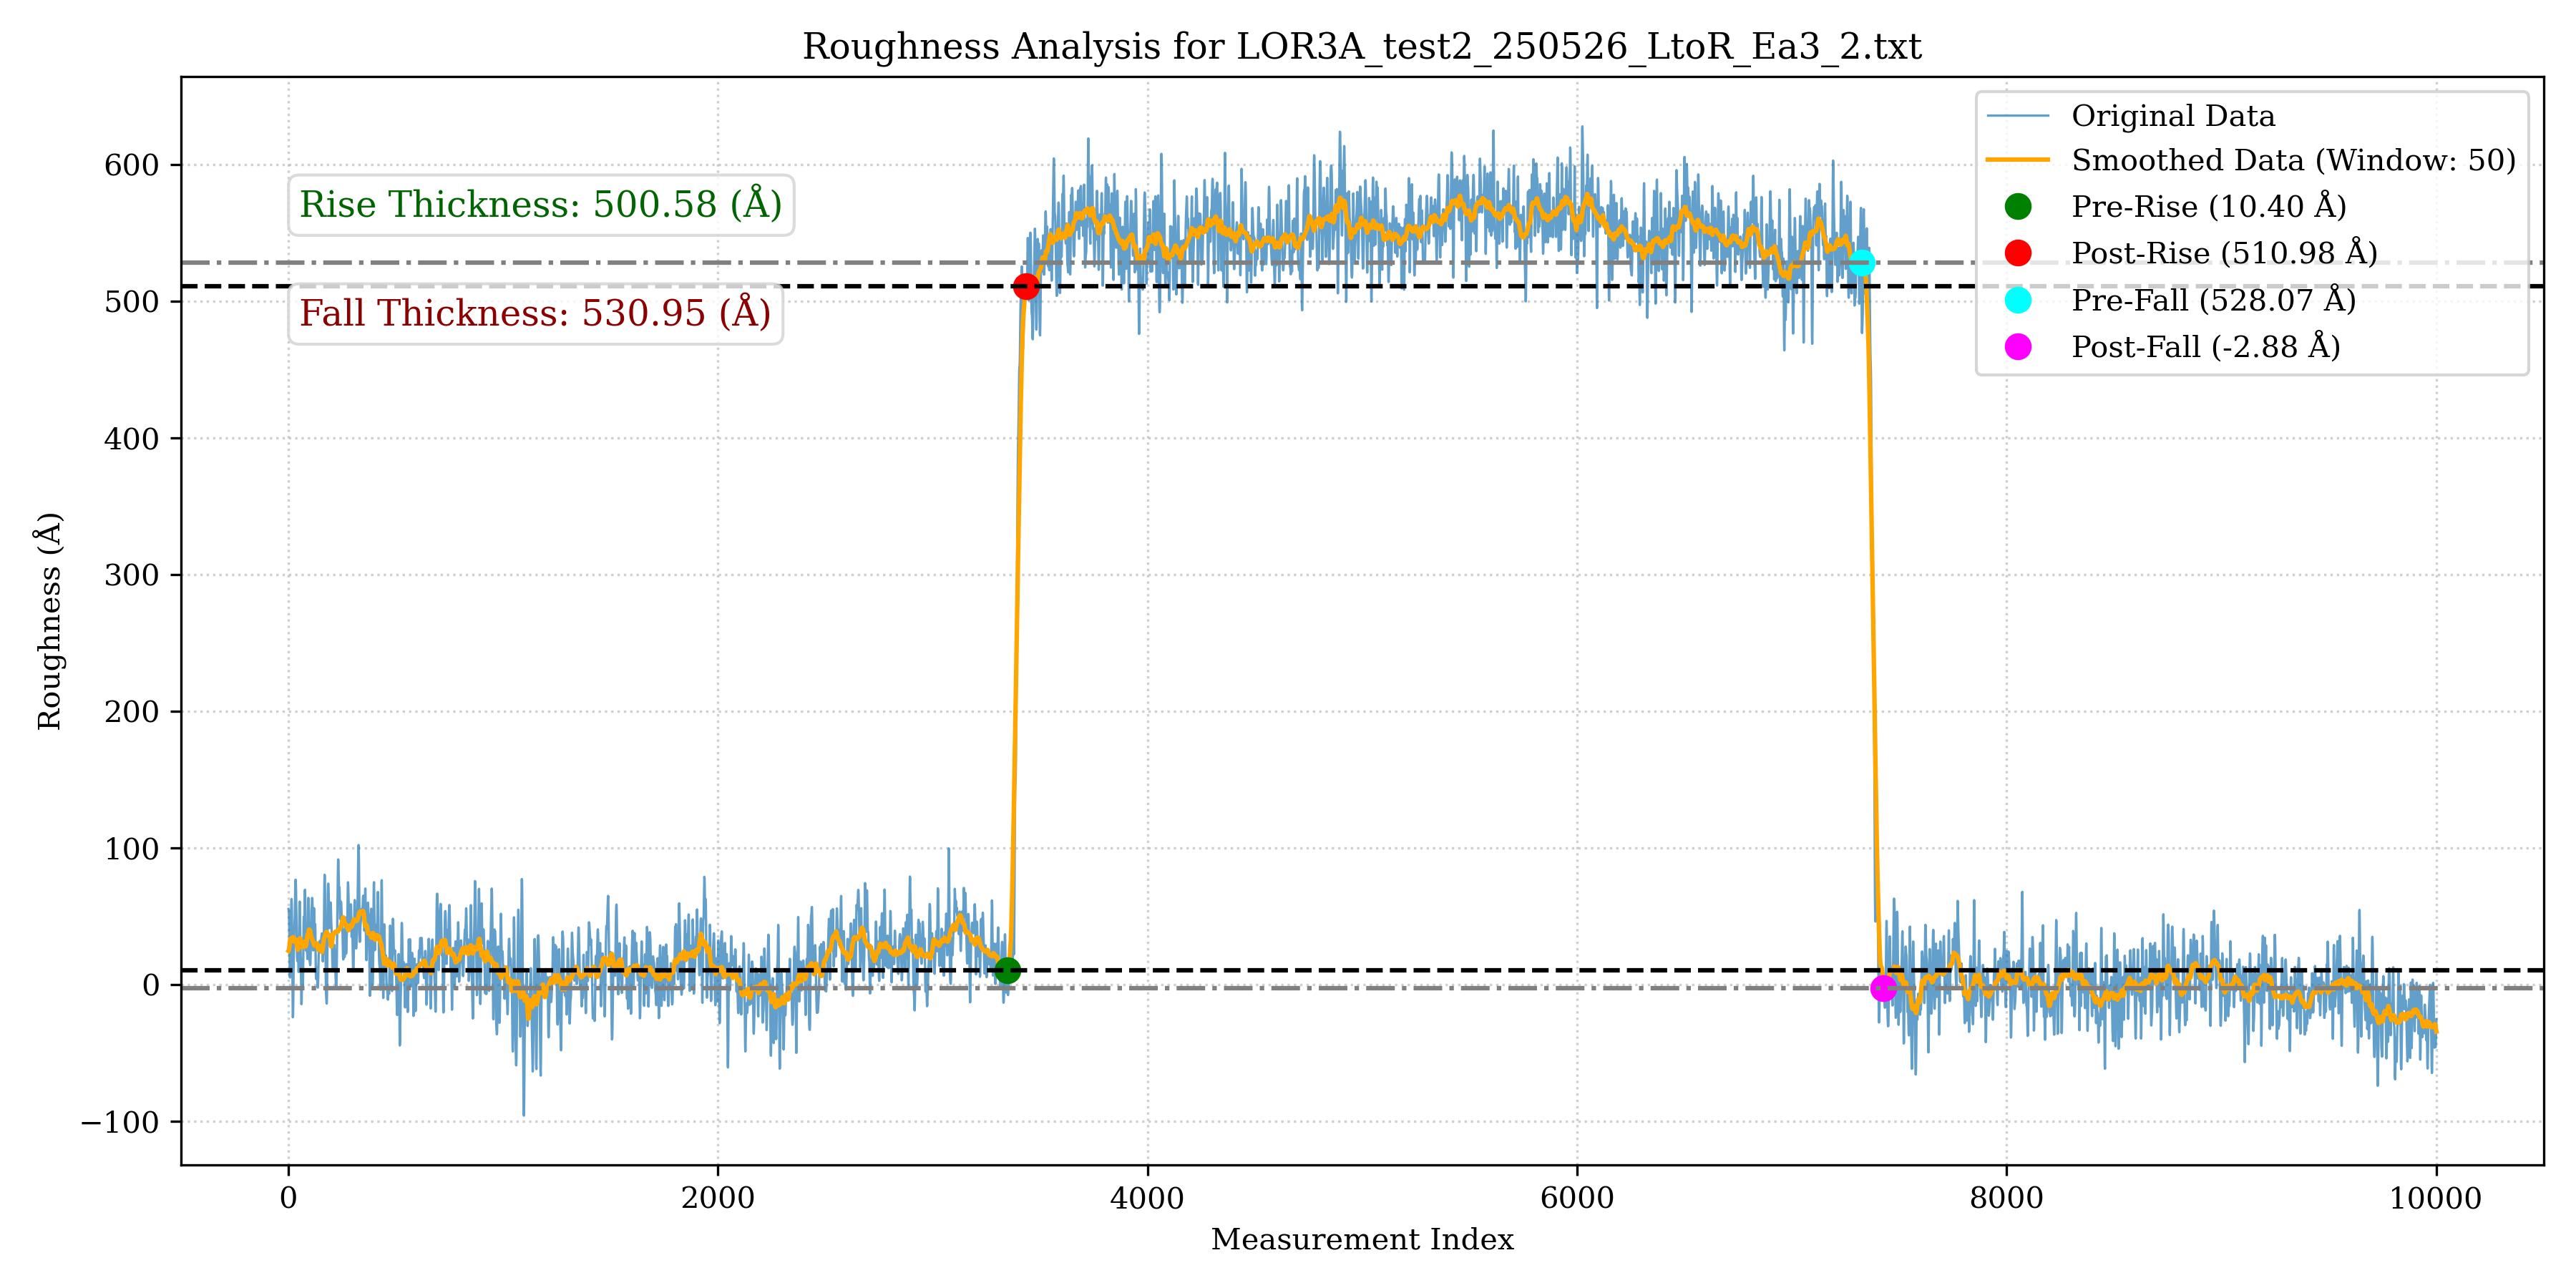
\includegraphics[width=\textwidth]{LOR3A_test2_250526_LtoR_Ea3_2.png}
    \label{fig:LOR3Atest2250526LtoREa32}
\end{figure}
\begin{figure}[H]
    \centering
    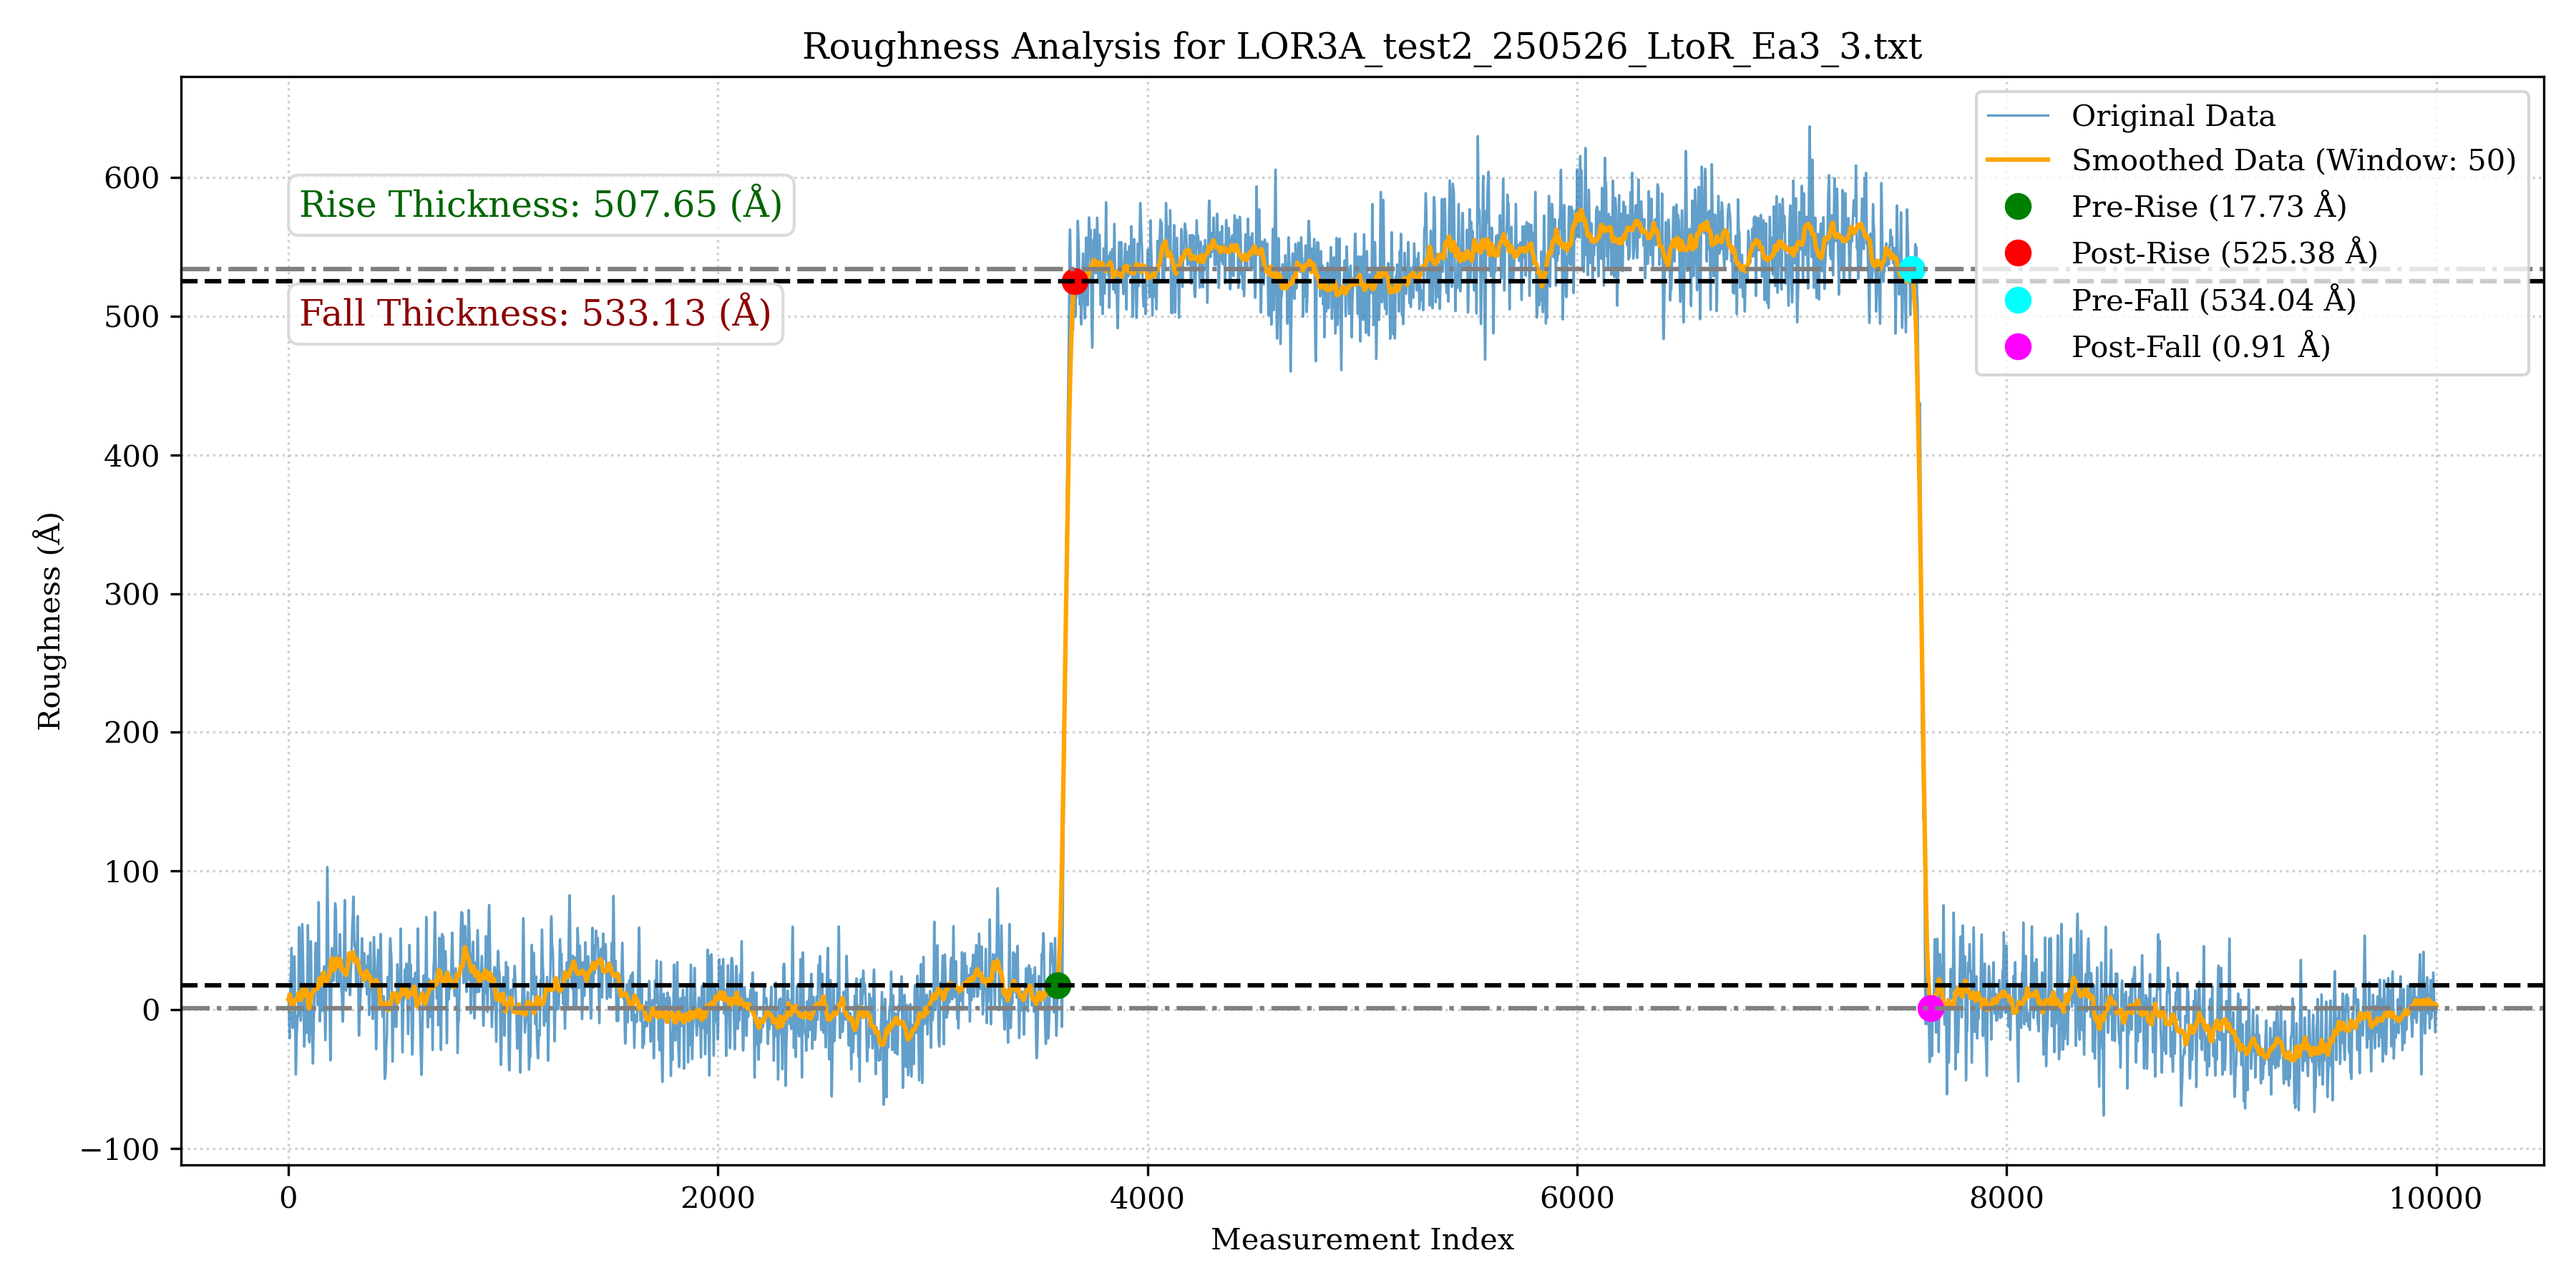
\includegraphics[width=\textwidth]{LOR3A_test2_250526_LtoR_Ea3_3.png}
    \label{fig:LOR3Atest2250526LtoREa33}
\end{figure}
\begin{figure}[H]
    \centering
    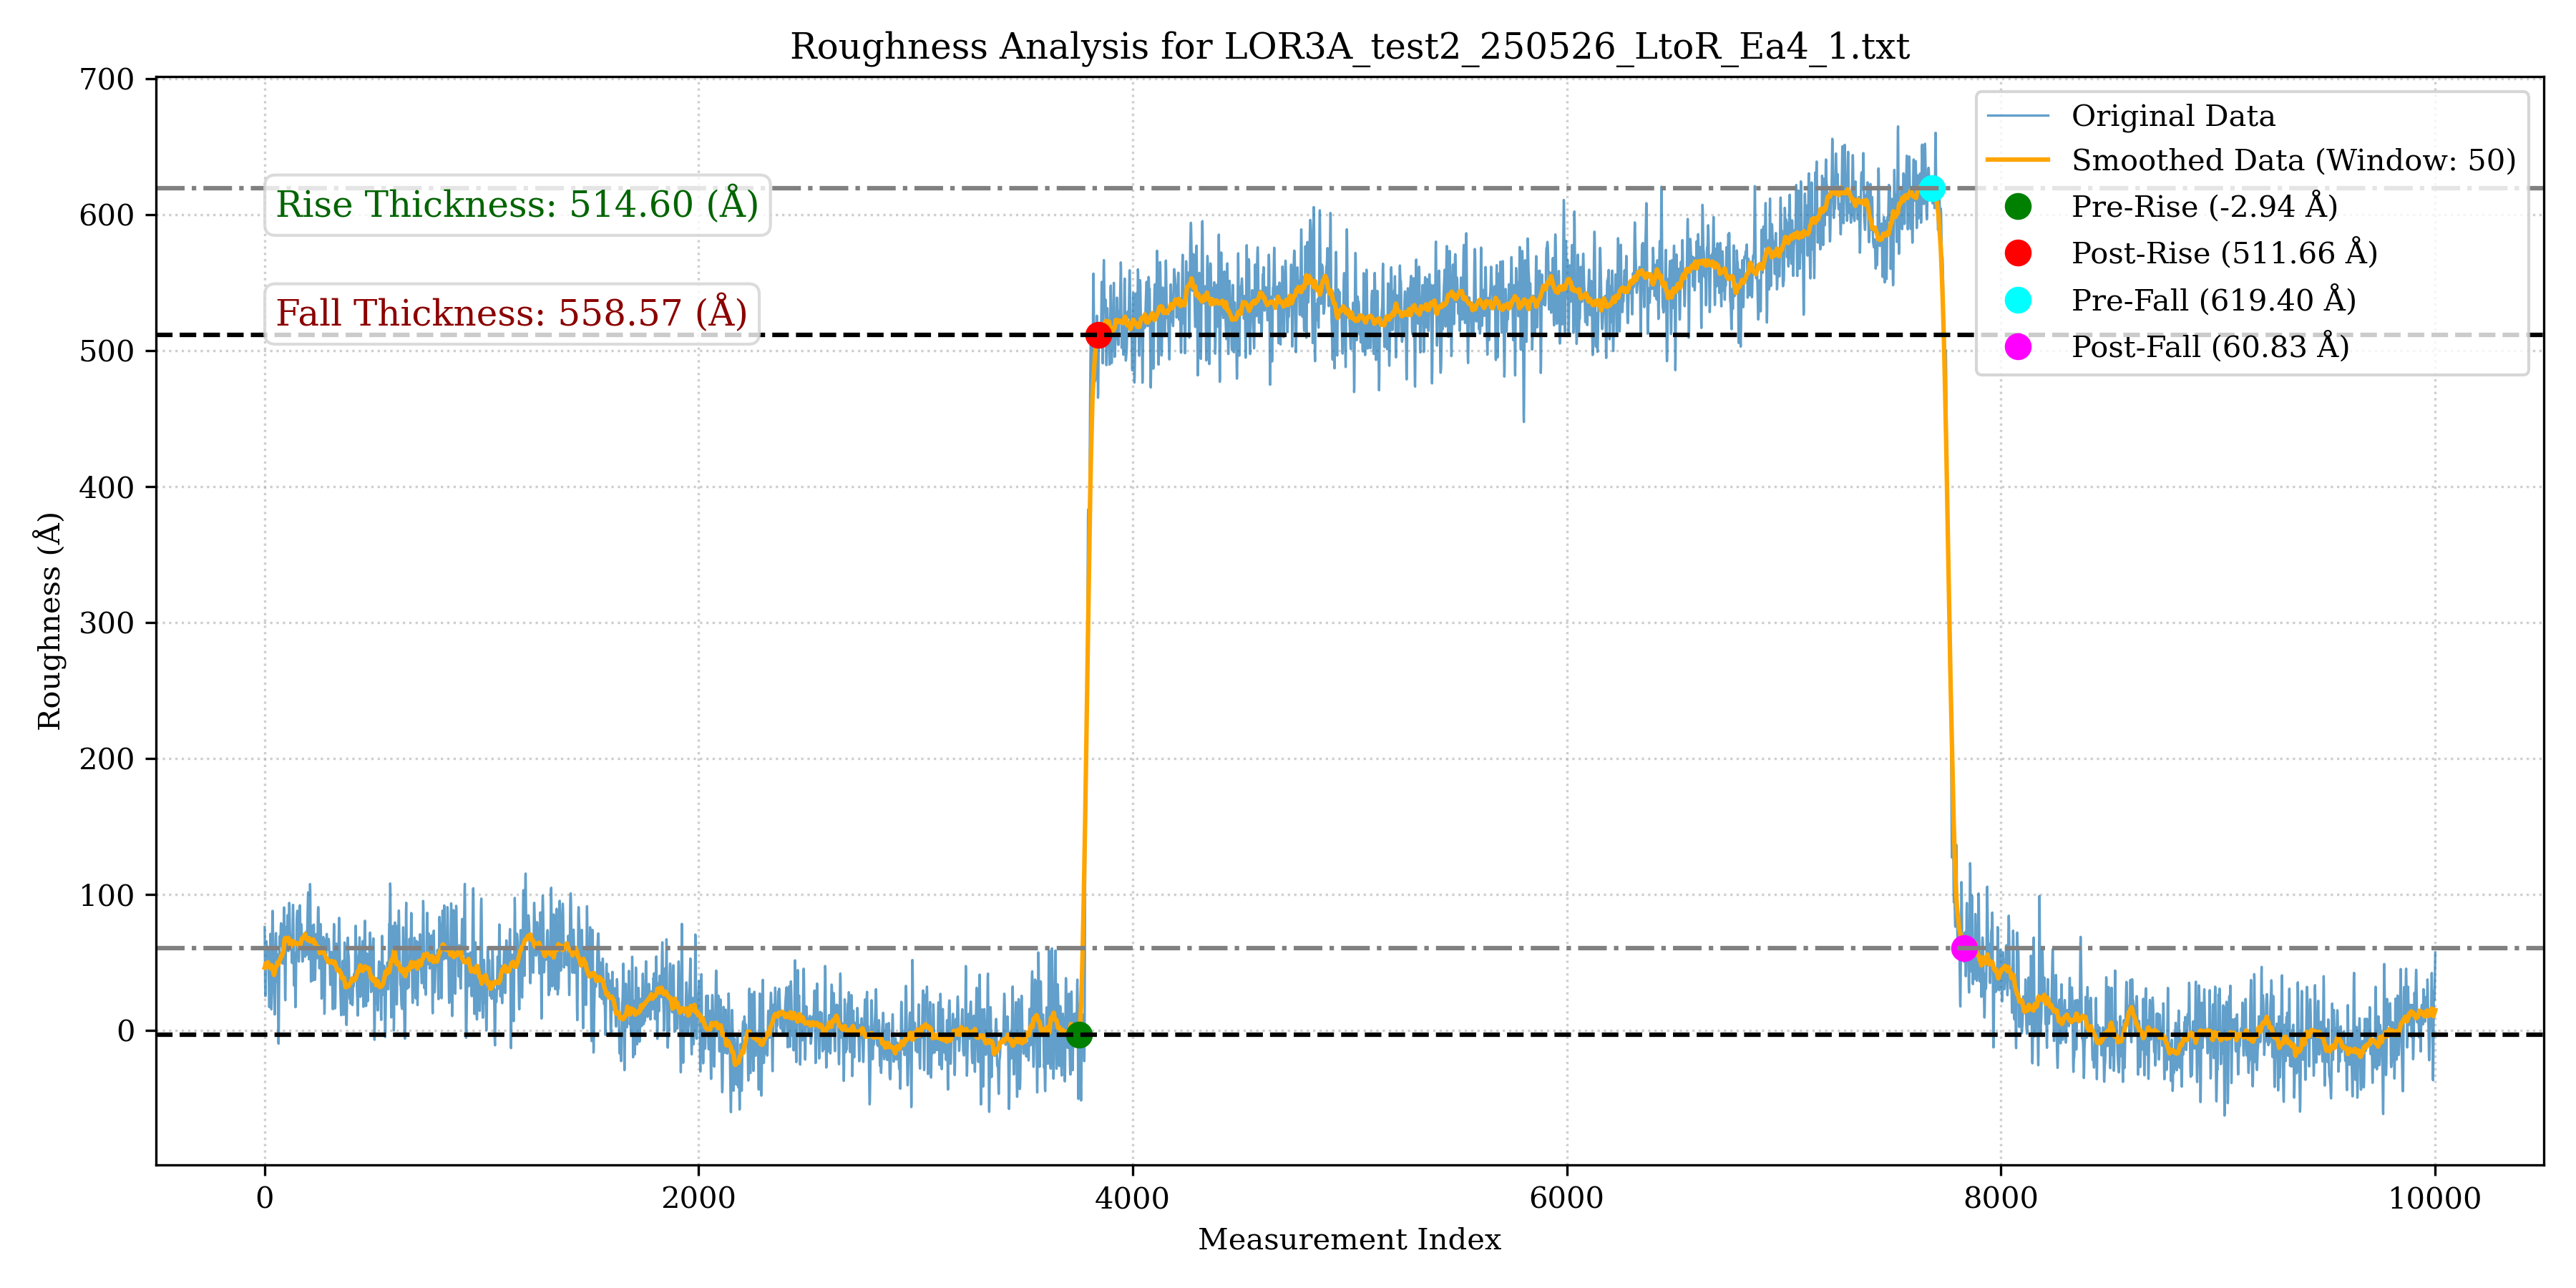
\includegraphics[width=\textwidth]{LOR3A_test2_250526_LtoR_Ea4_1.png}
    \label{fig:LOR3Atest2250526LtoREa41}
\end{figure}
\begin{figure}[H]
    \centering
    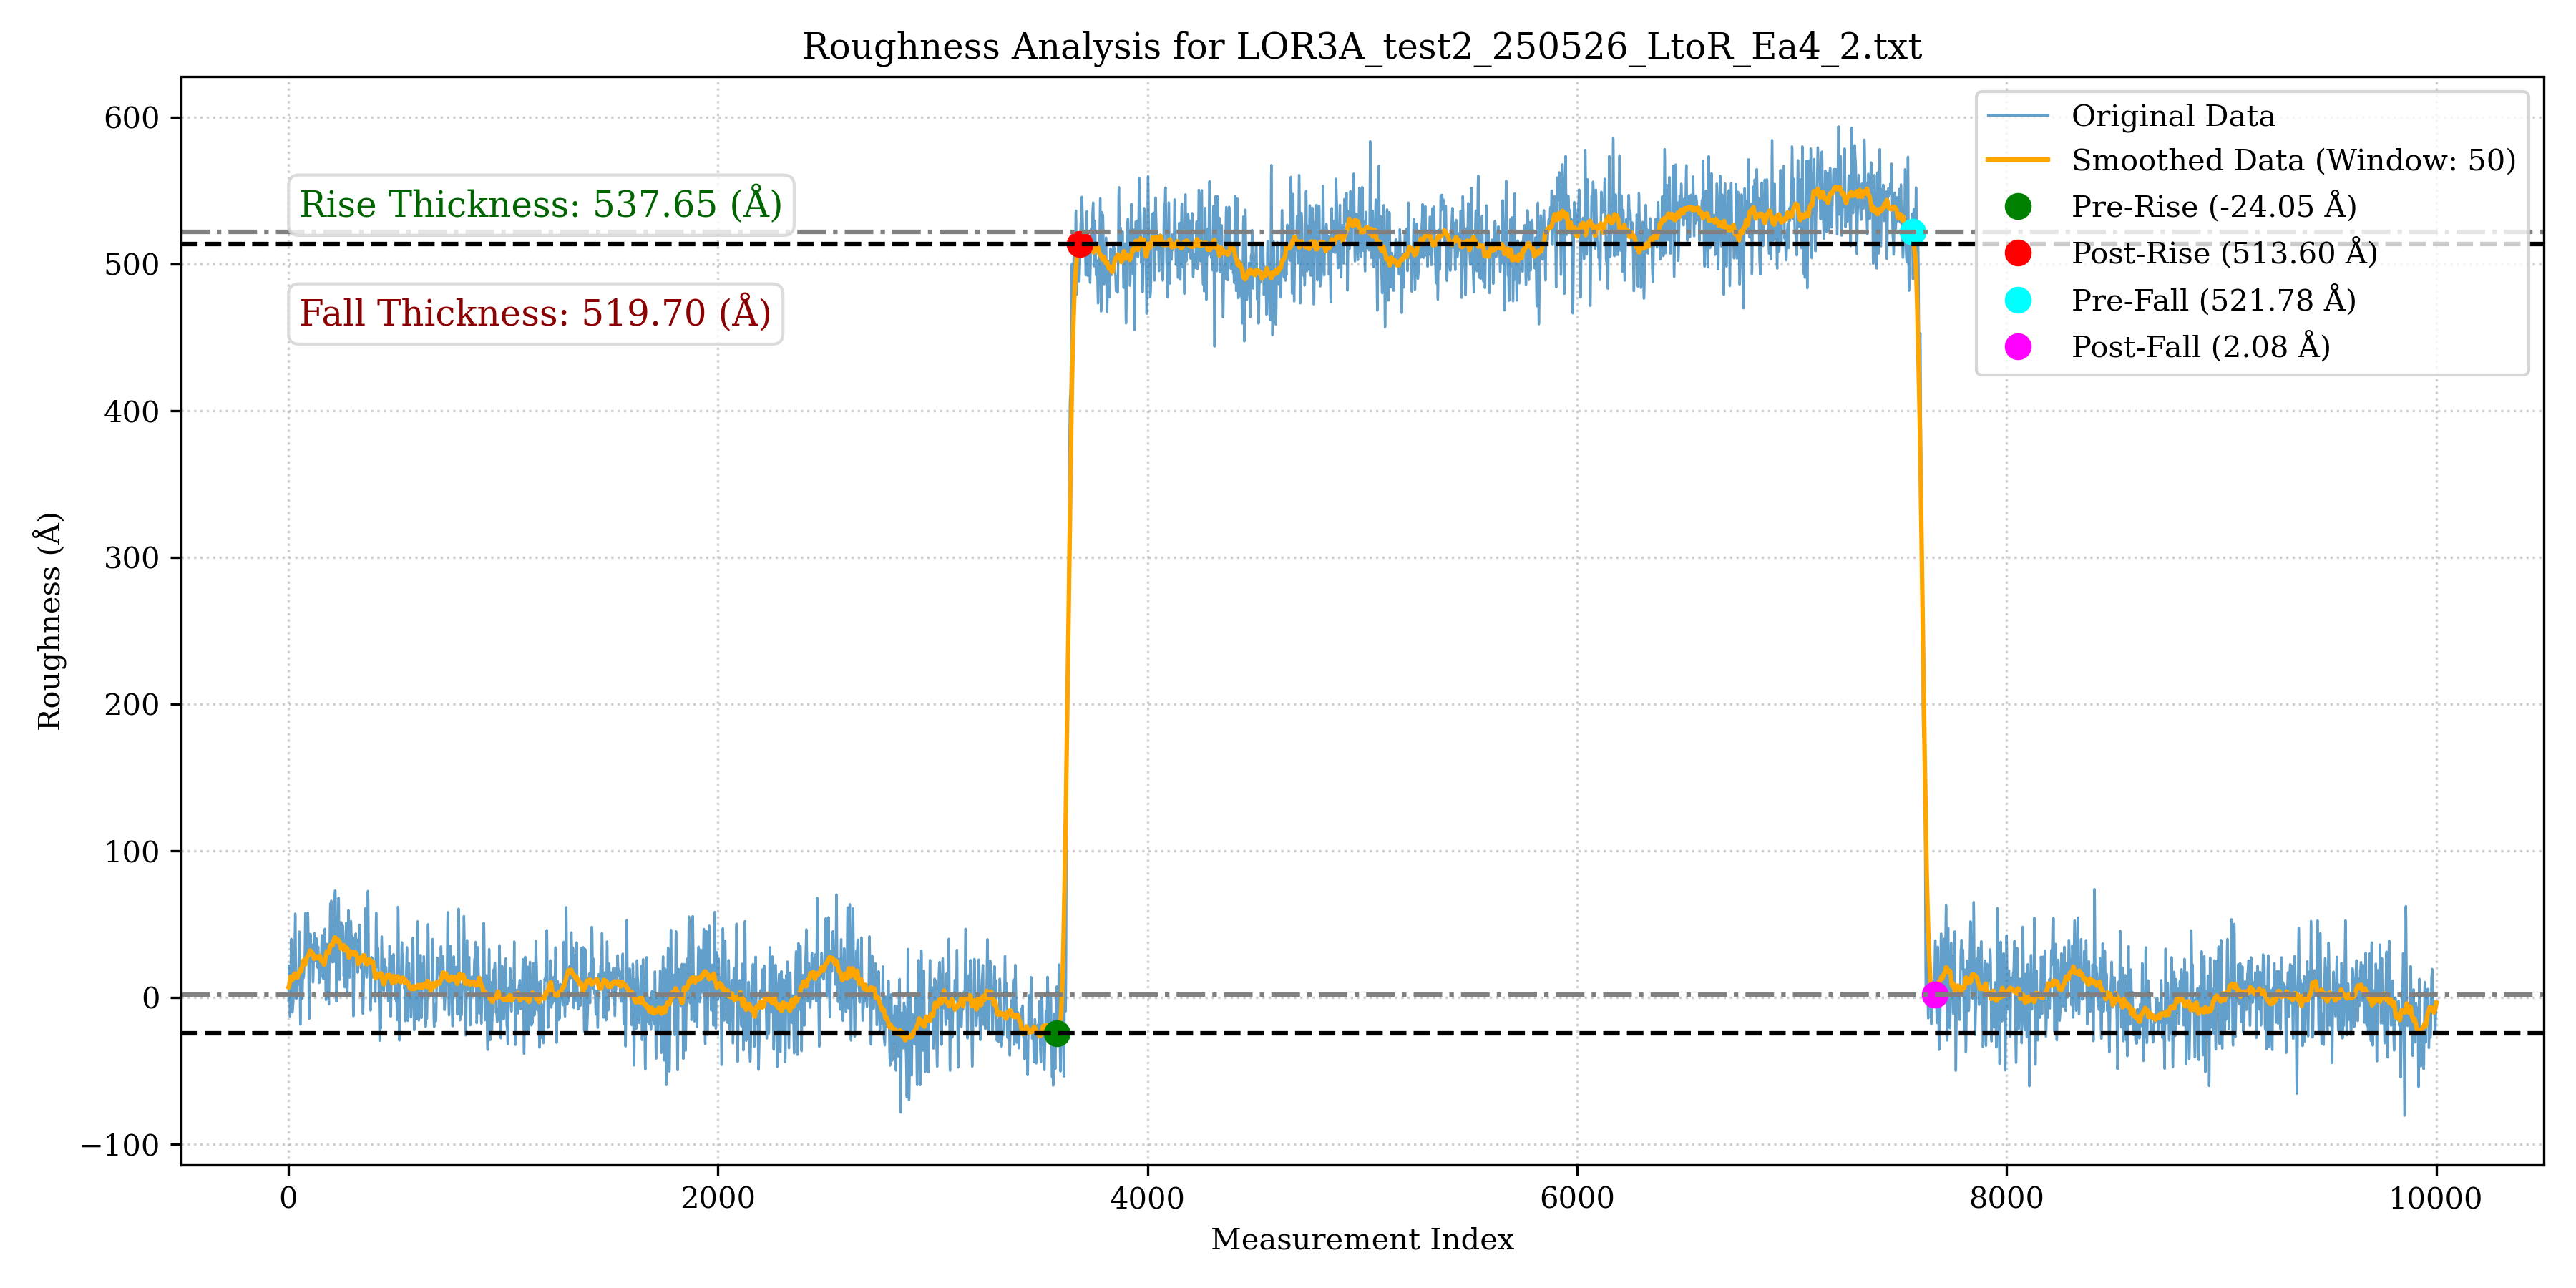
\includegraphics[width=\textwidth]{LOR3A_test2_250526_LtoR_Ea4_2.png}
    \label{fig:LOR3Atest2250526LtoREa42}
\end{figure}
\begin{figure}[H]
    \centering
    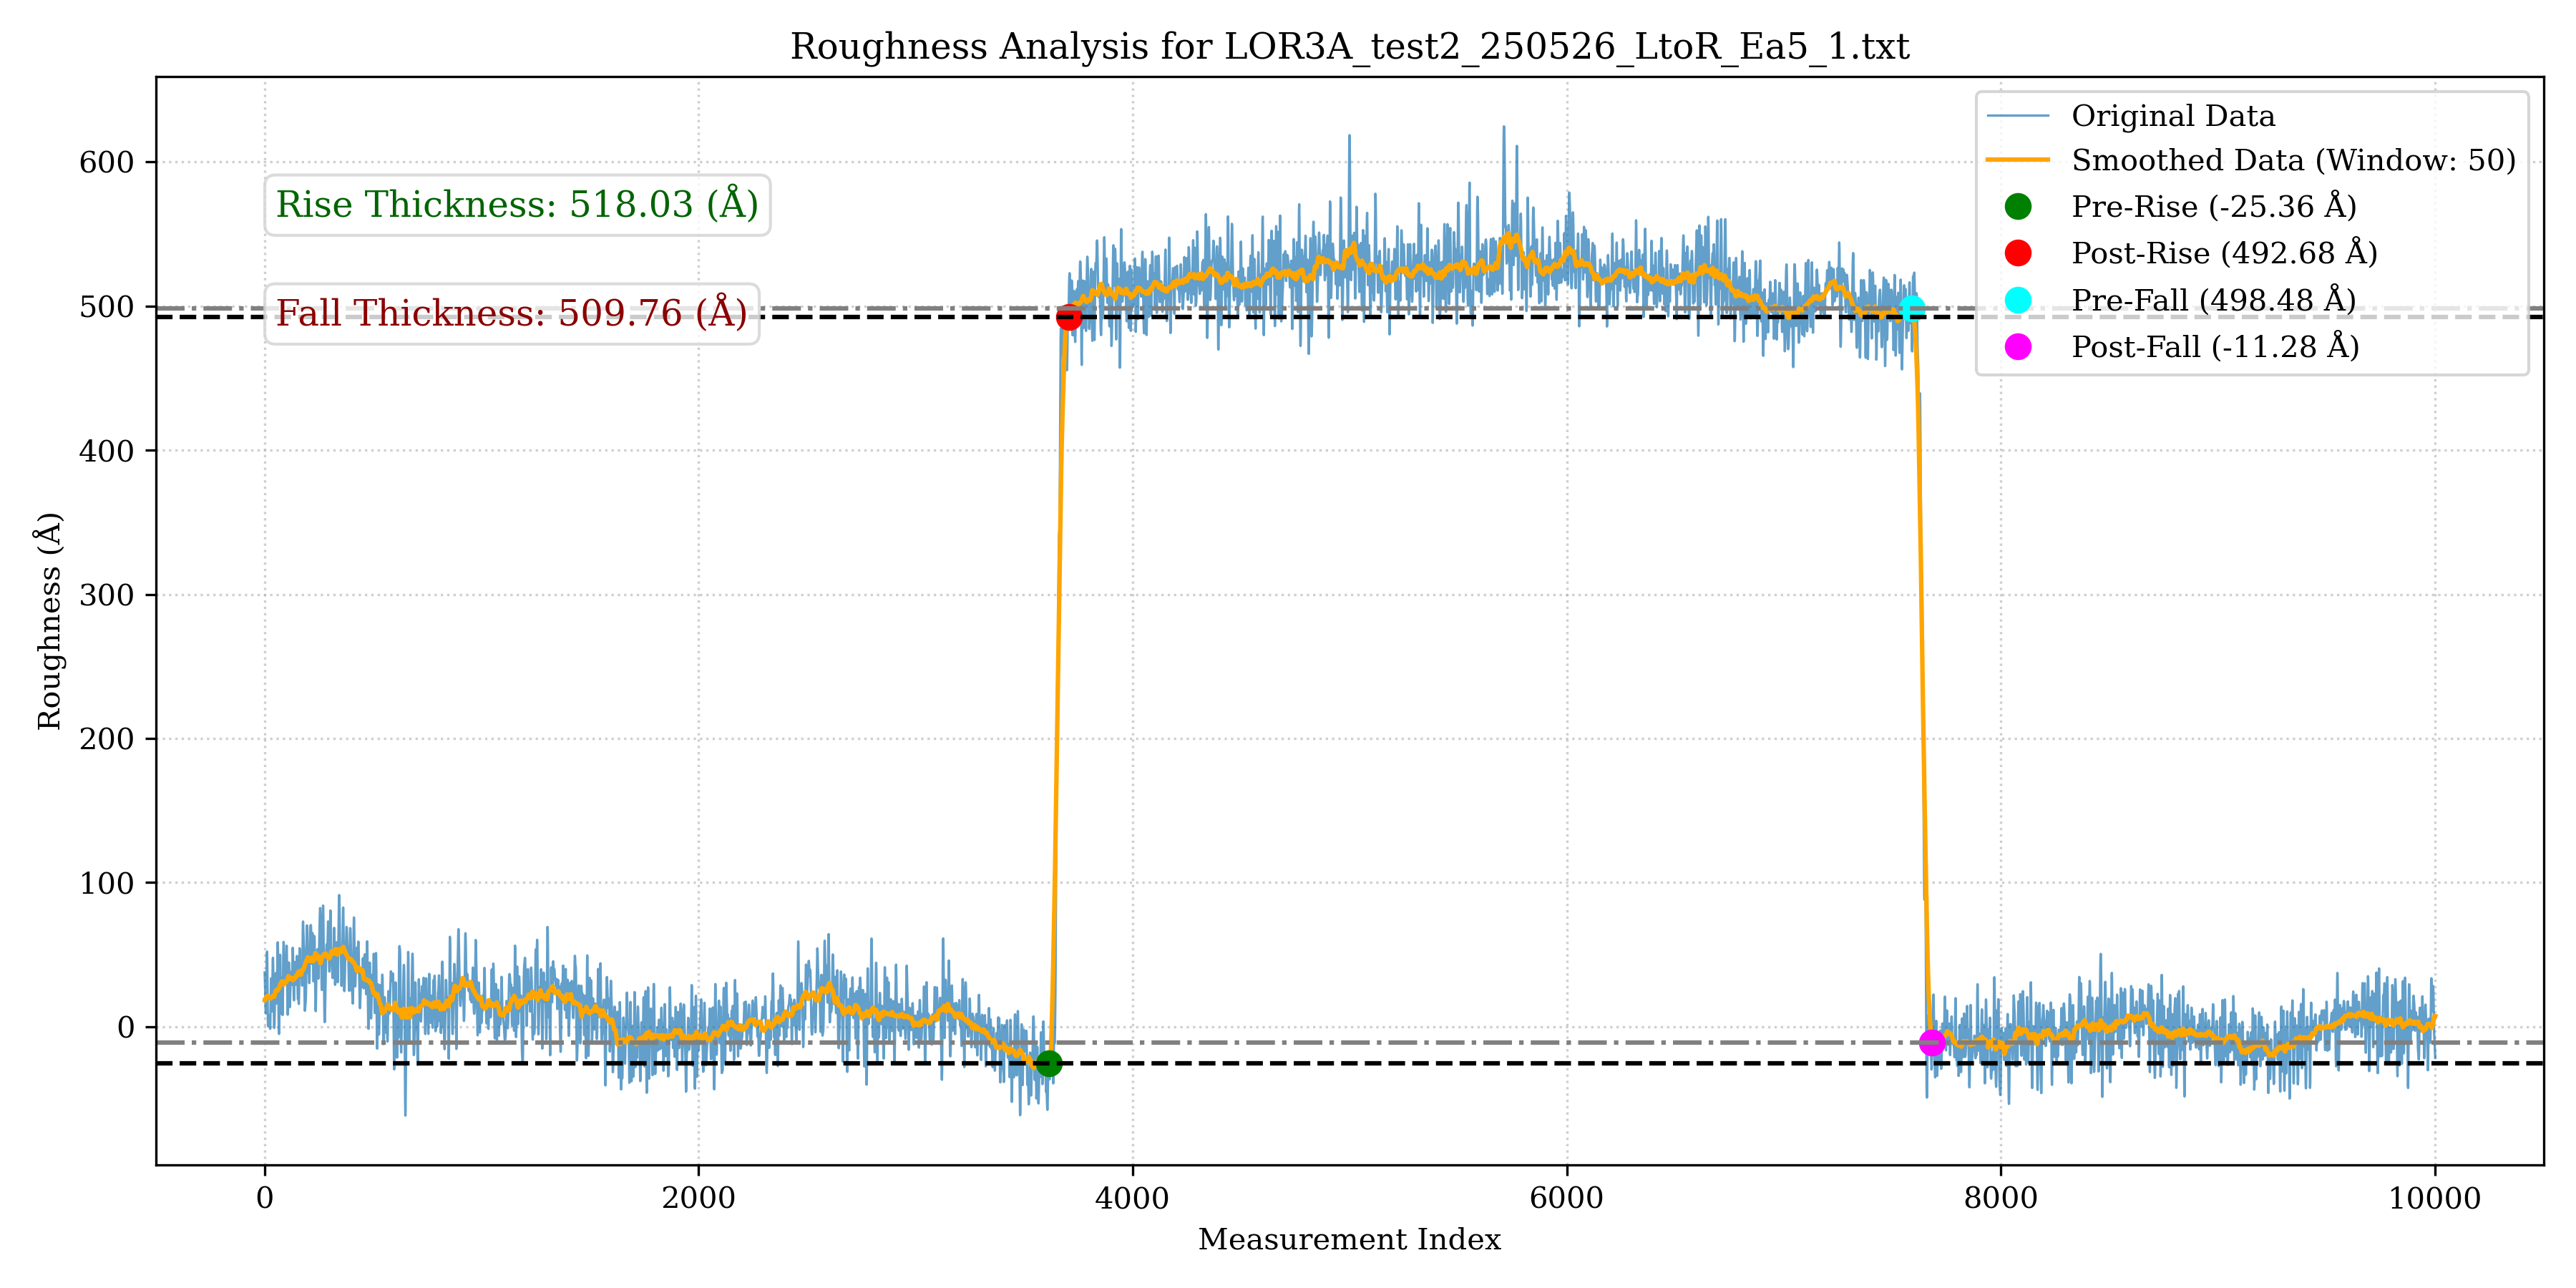
\includegraphics[width=\textwidth]{LOR3A_test2_250526_LtoR_Ea5_1.png}
    \label{fig:LOR3Atest2250526LtoREa51}
\end{figure}
\begin{figure}[H]
    \centering
    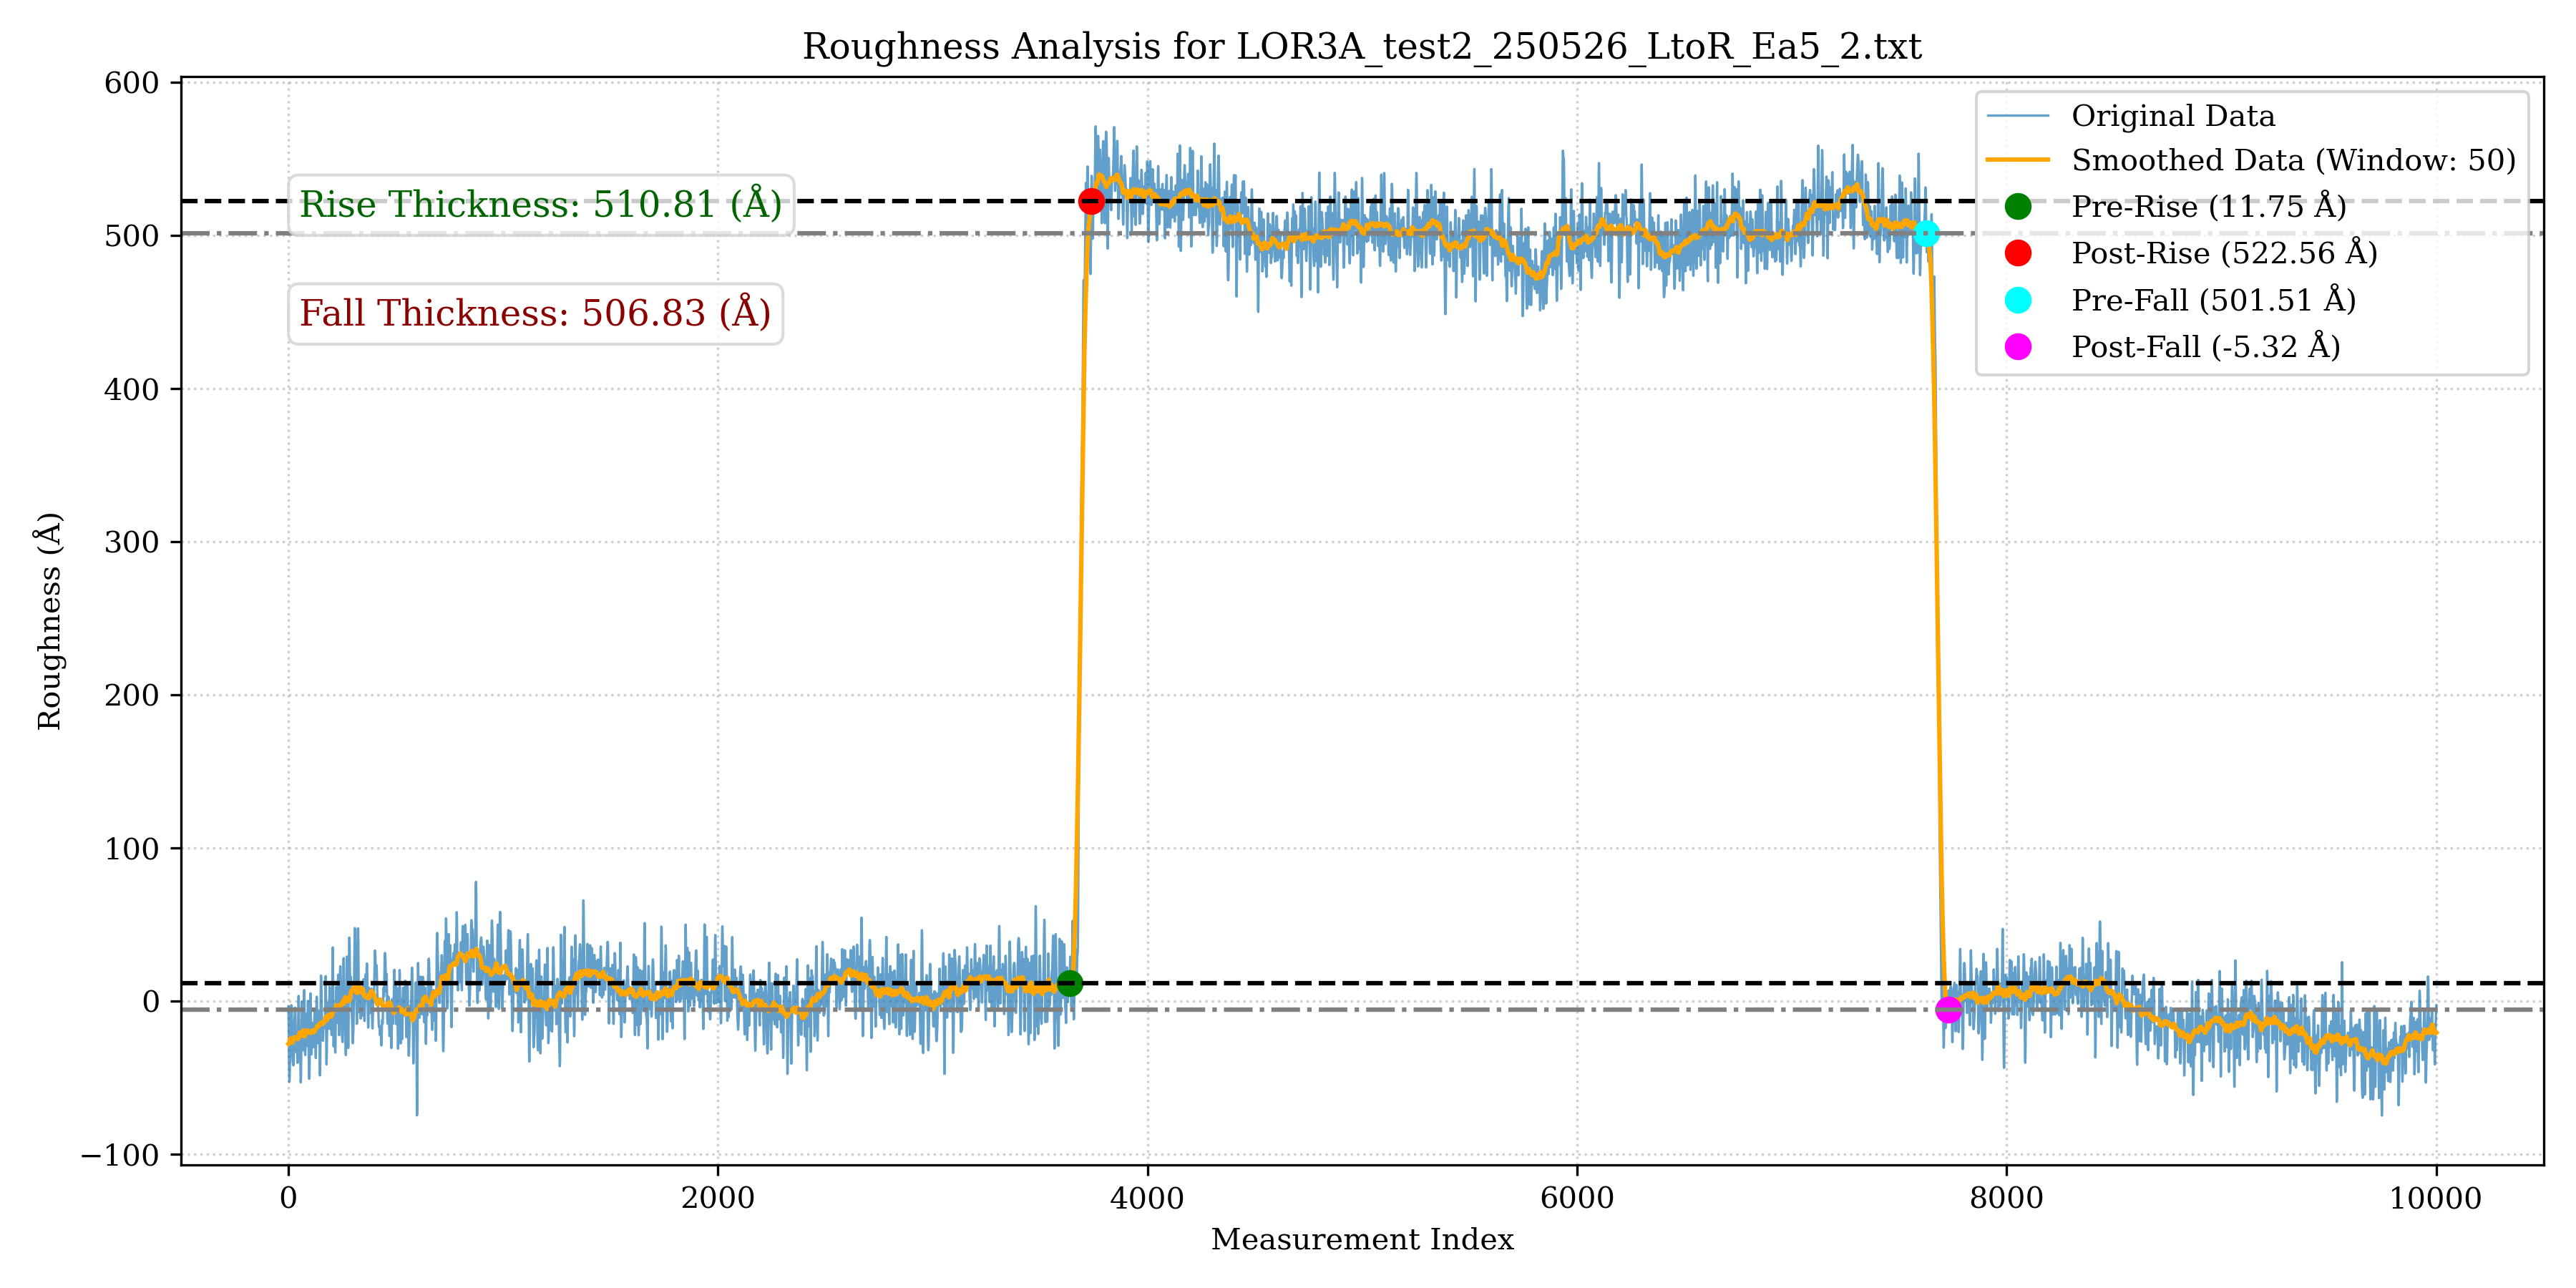
\includegraphics[width=\textwidth]{LOR3A_test2_250526_LtoR_Ea5_2.png}
    \label{fig:LOR3Atest2250526LtoREa52}
\end{figure}
\begin{figure}[H]
    \centering
    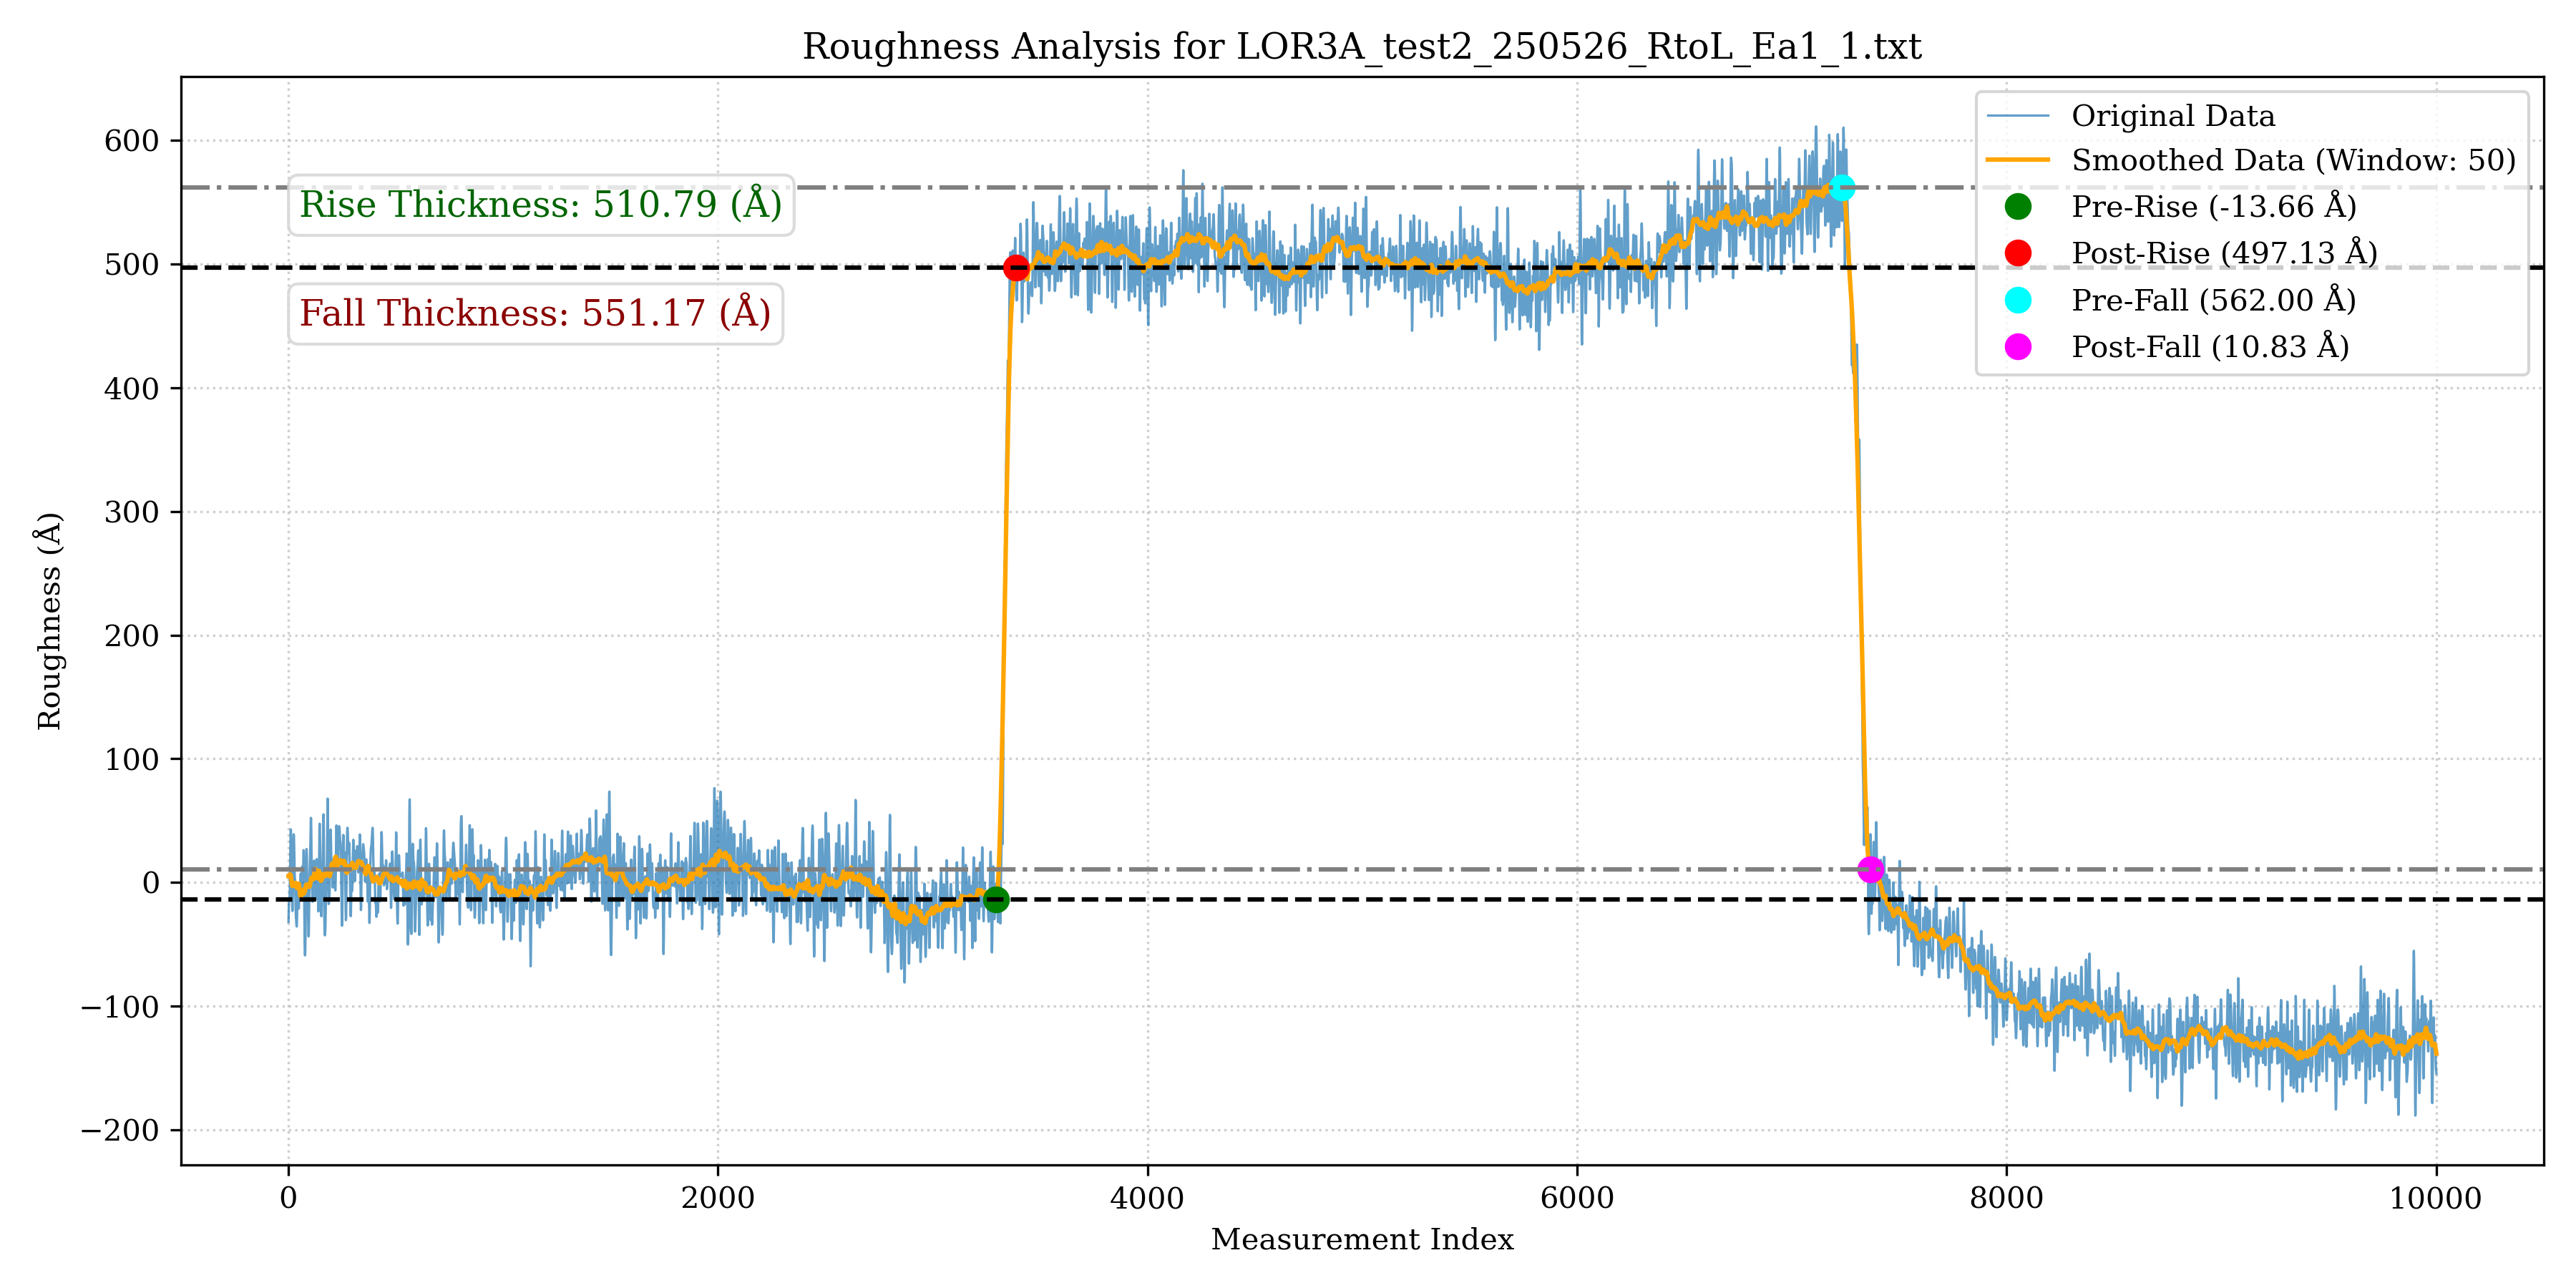
\includegraphics[width=\textwidth]{LOR3A_test2_250526_RtoL_Ea1_1.png}
    \label{fig:LOR3Atest2250526RtoLEa11}
\end{figure}
\begin{figure}[H]
    \centering
    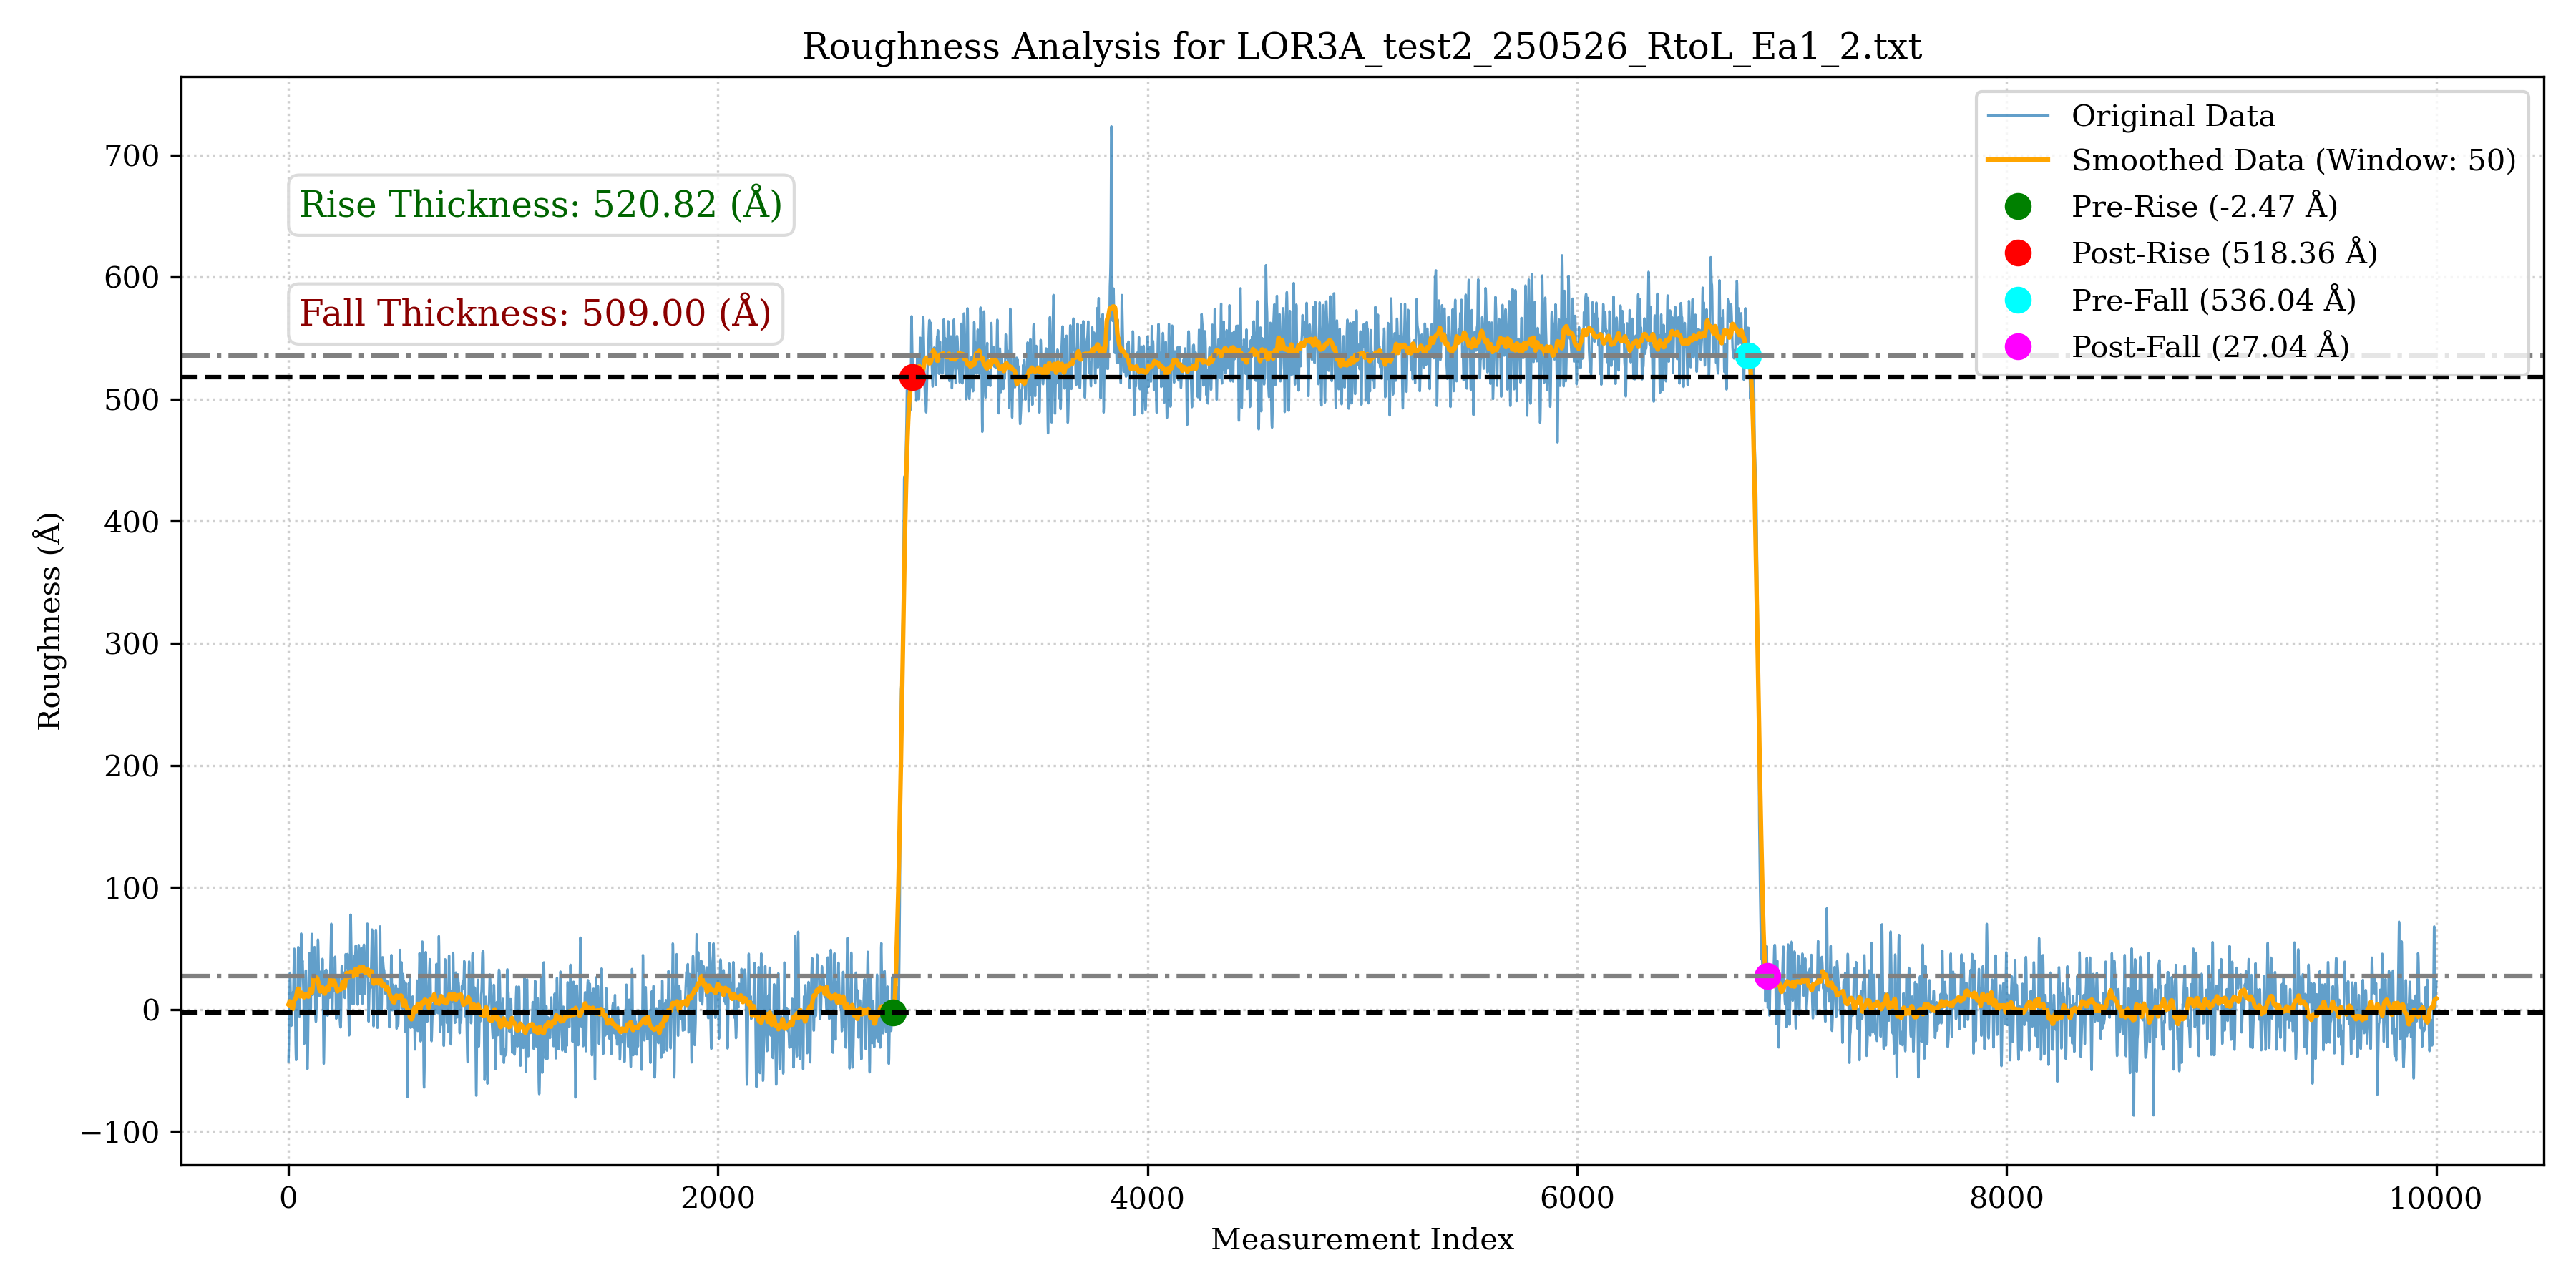
\includegraphics[width=\textwidth]{LOR3A_test2_250526_RtoL_Ea1_2.png}
    \label{fig:LOR3Atest2250526RtoLEa12}
\end{figure}
\begin{figure}[H]
    \centering
    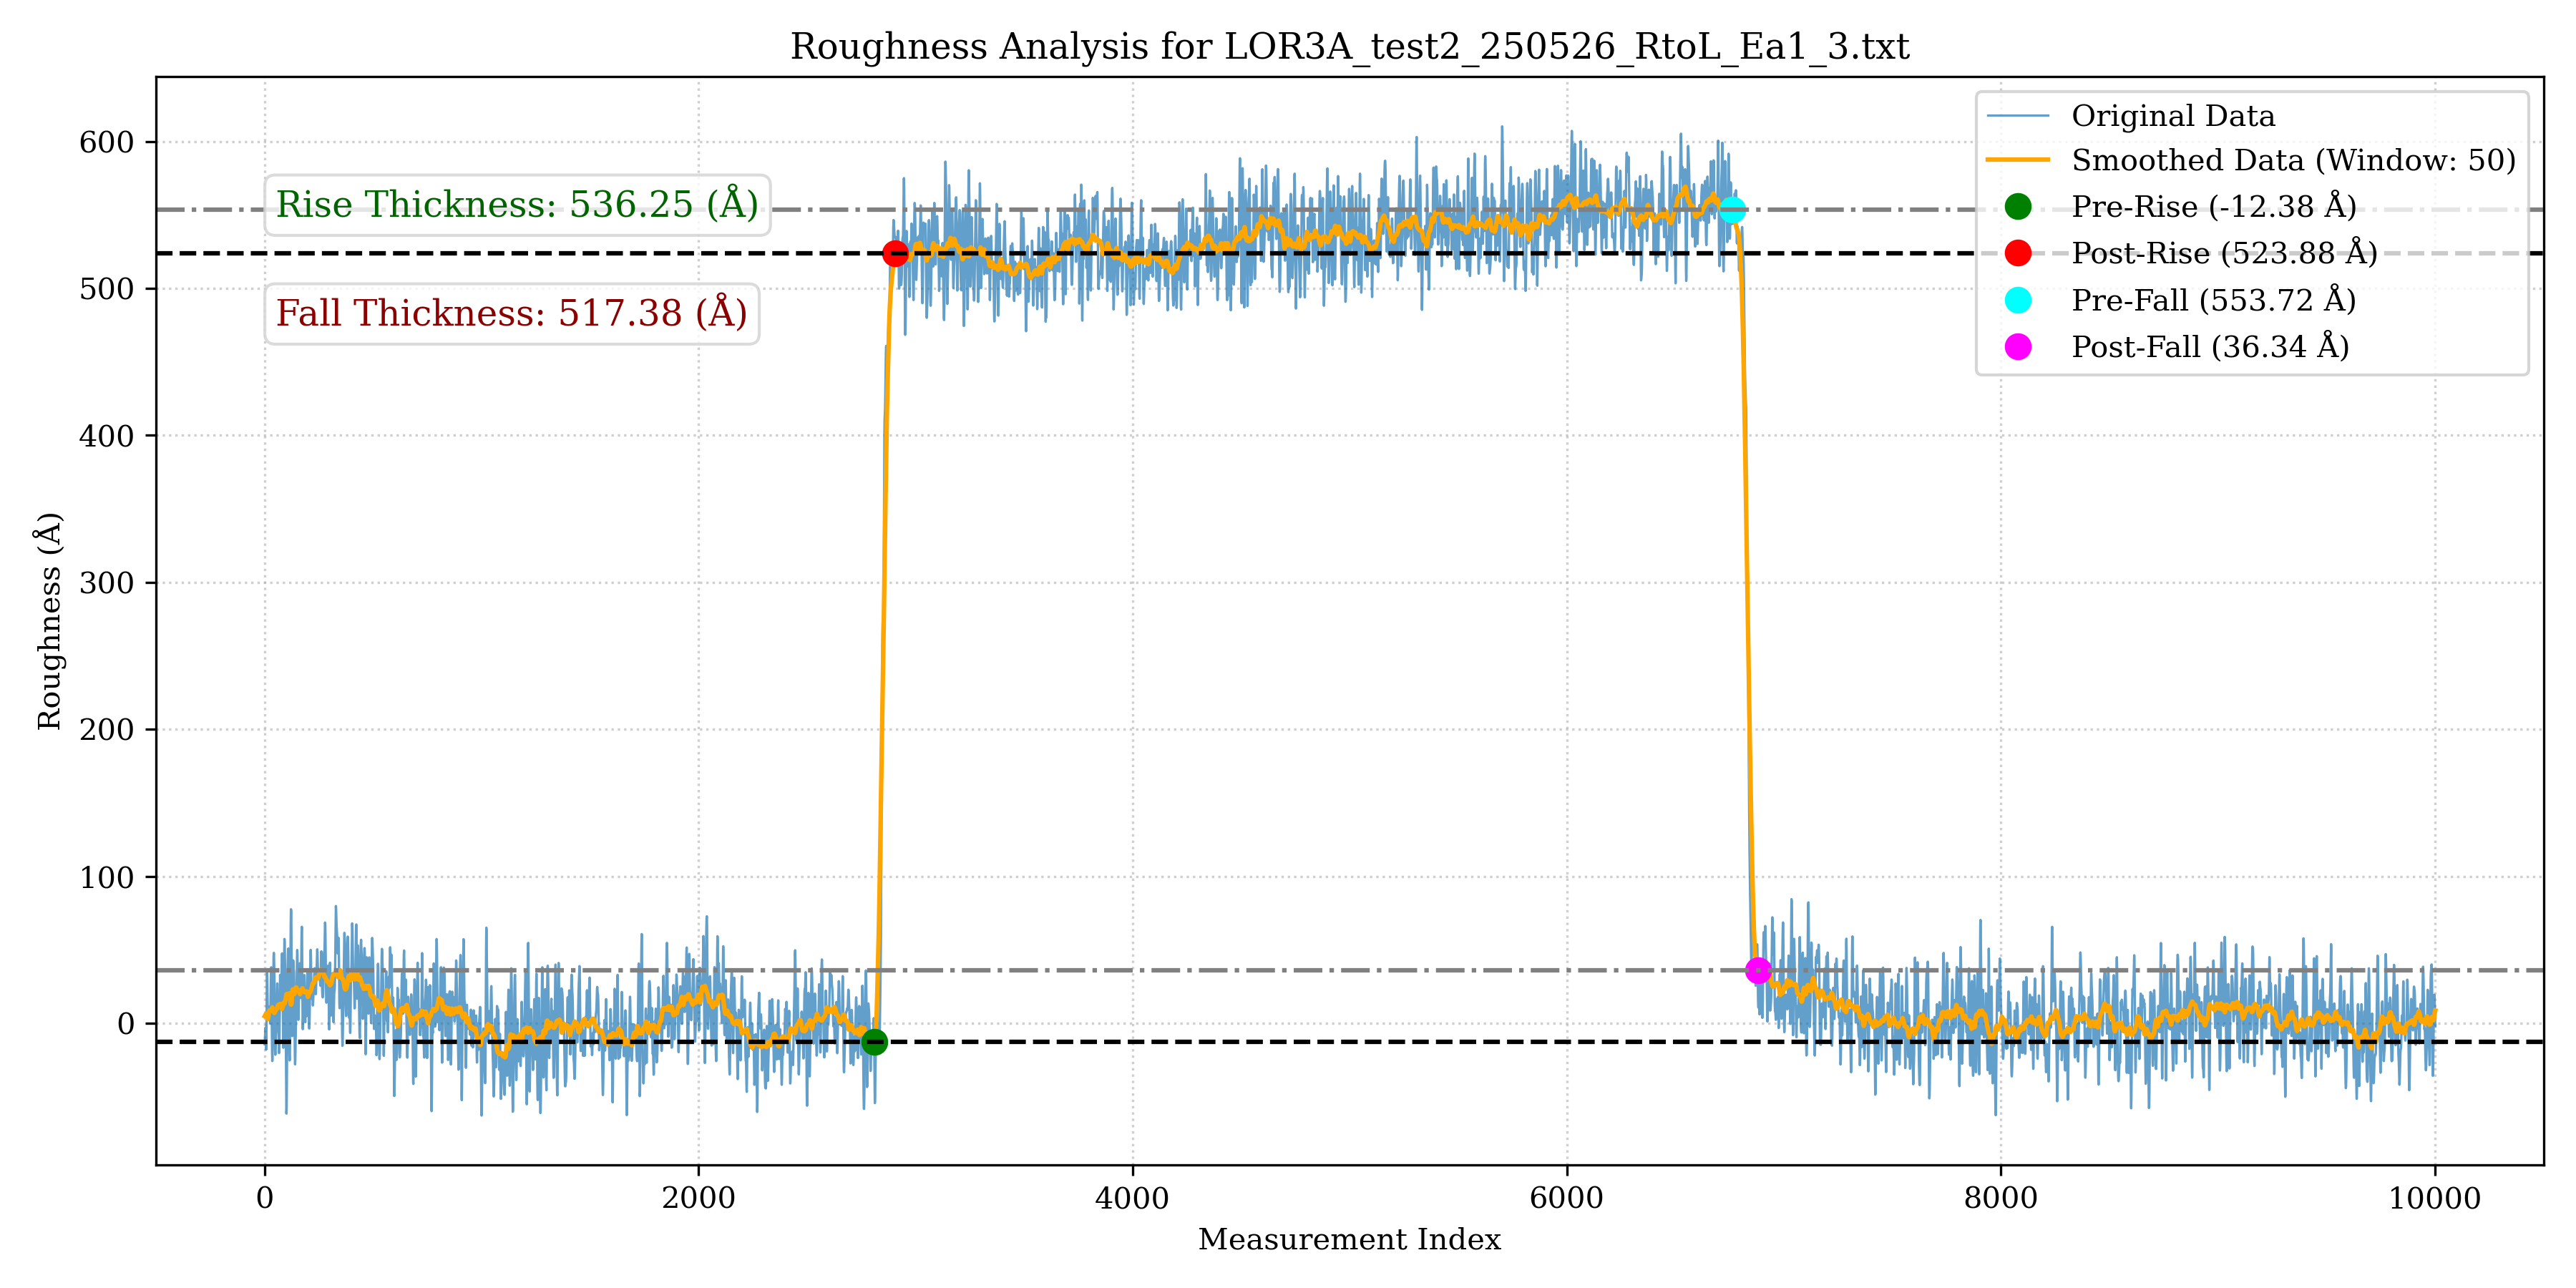
\includegraphics[width=\textwidth]{LOR3A_test2_250526_RtoL_Ea1_3.png}
    \label{fig:LOR3Atest2250526RtoLEa13}
\end{figure}
\begin{figure}[H]
    \centering
    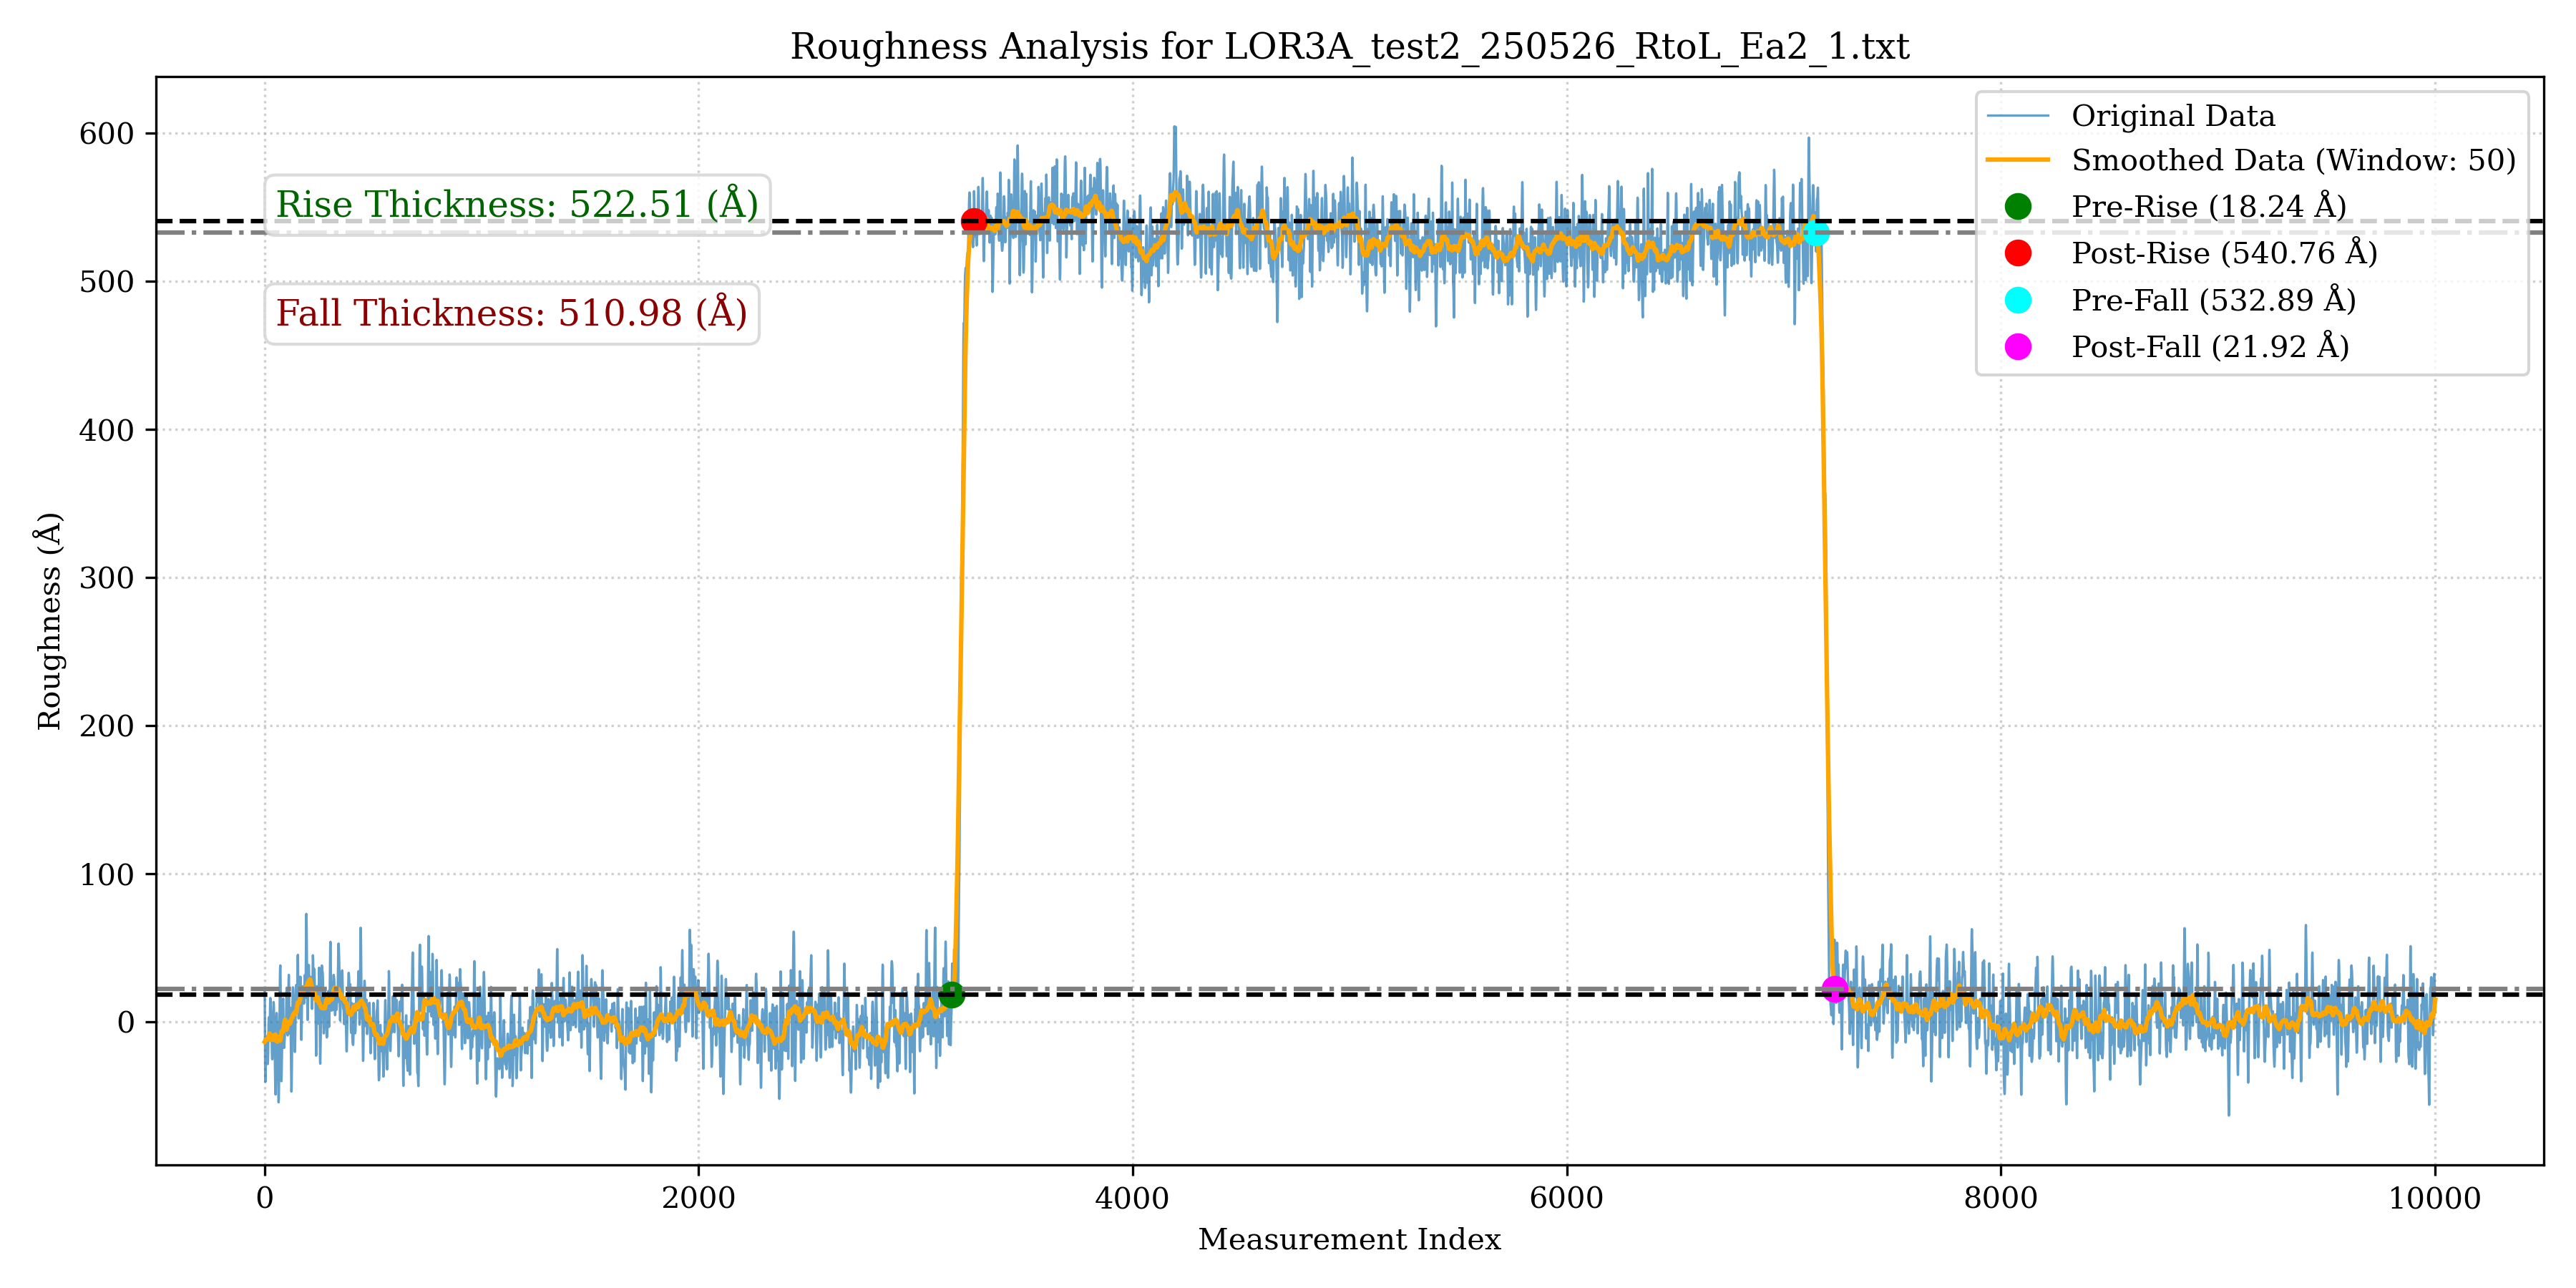
\includegraphics[width=\textwidth]{LOR3A_test2_250526_RtoL_Ea2_1.png}
    \label{fig:LOR3Atest2250526RtoLEa21}
\end{figure}
\begin{figure}[H]
    \centering
    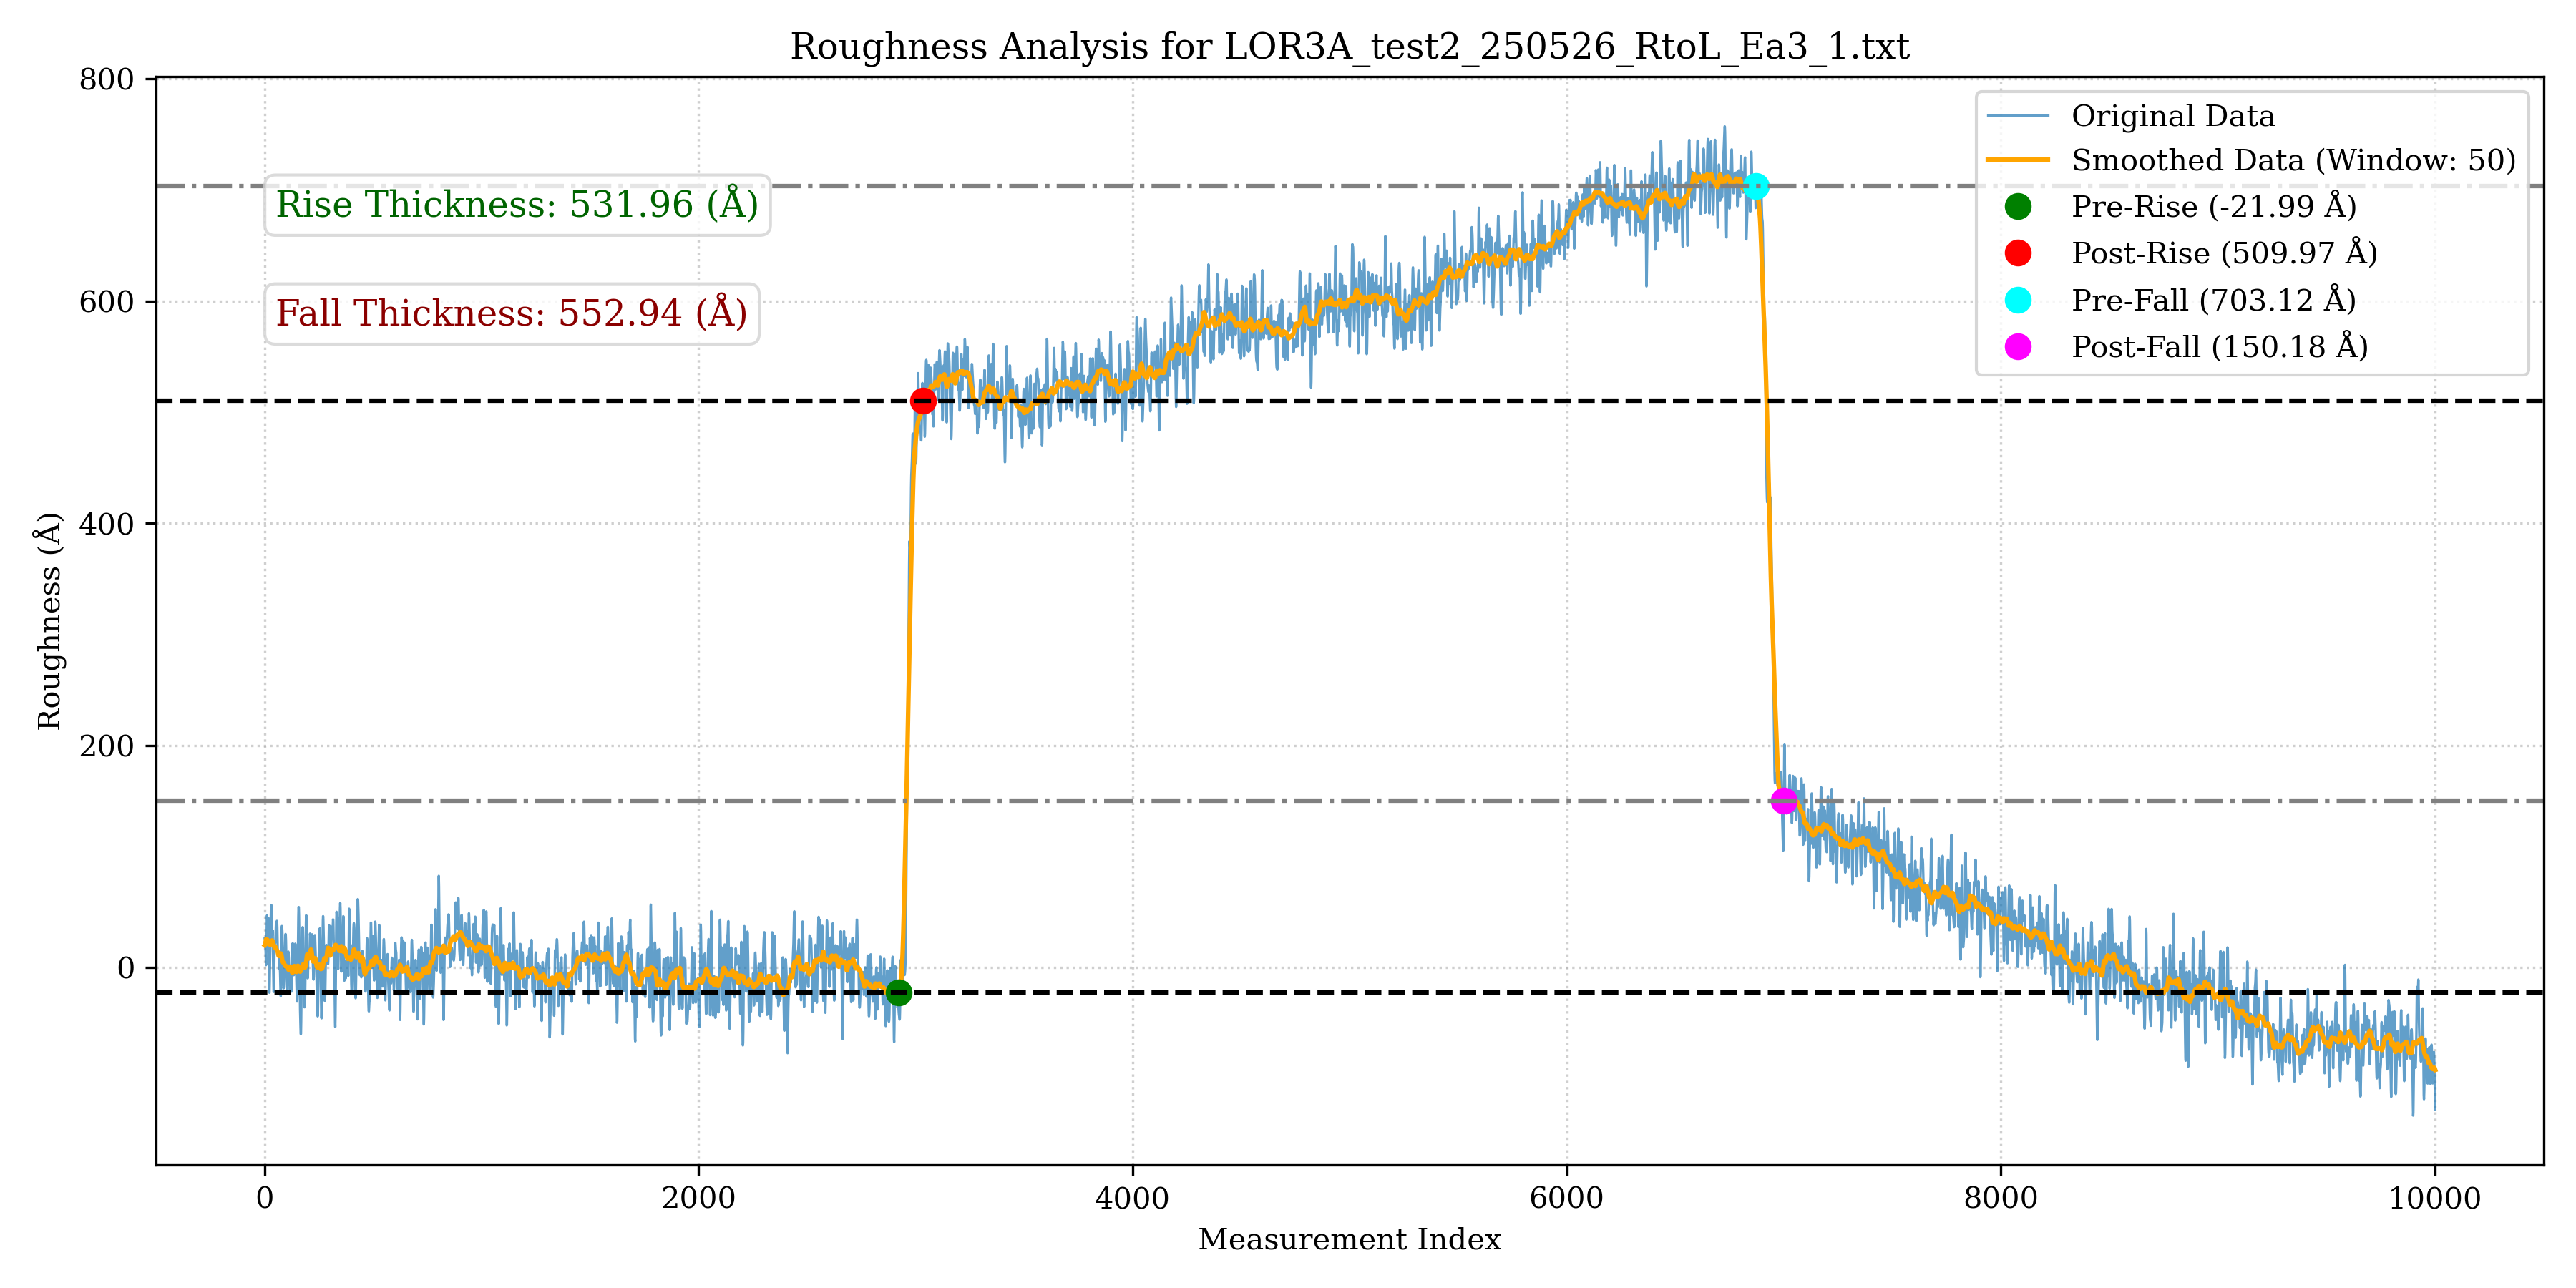
\includegraphics[width=\textwidth]{LOR3A_test2_250526_RtoL_Ea3_1.png}
    \label{fig:LOR3Atest2250526RtoLEa31}
\end{figure}
\begin{figure}[H]
    \centering
    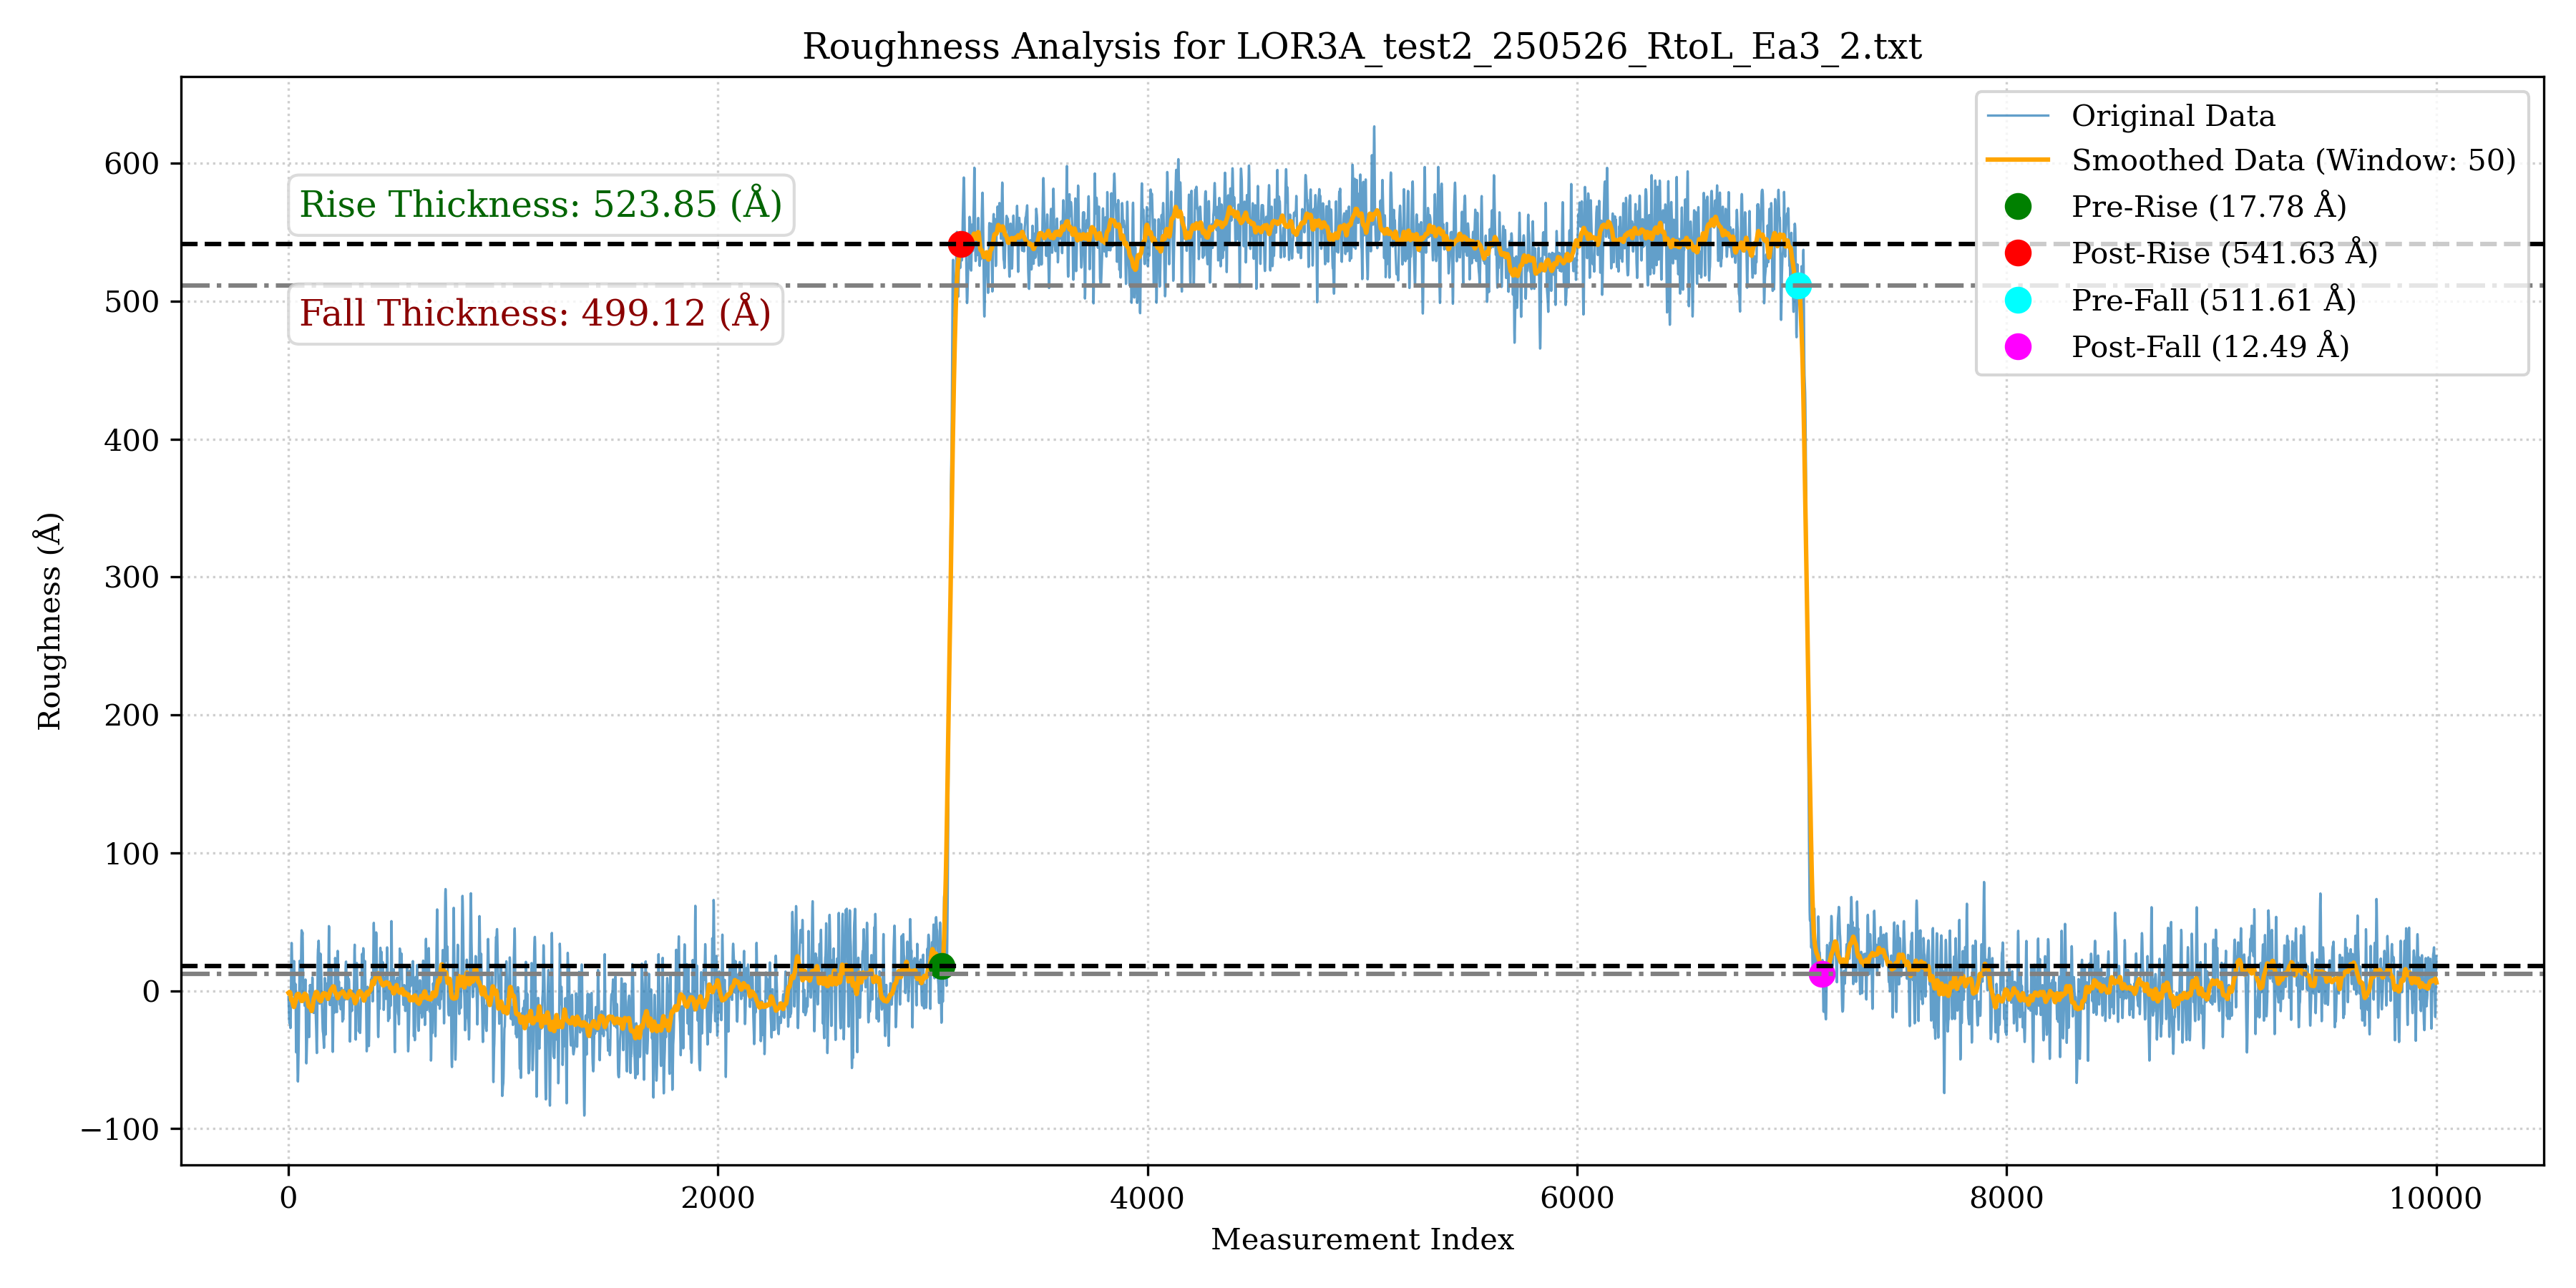
\includegraphics[width=\textwidth]{LOR3A_test2_250526_RtoL_Ea3_2.png}
    \label{fig:LOR3Atest2250526RtoLEa32}
\end{figure}
\begin{figure}[H]
    \centering
    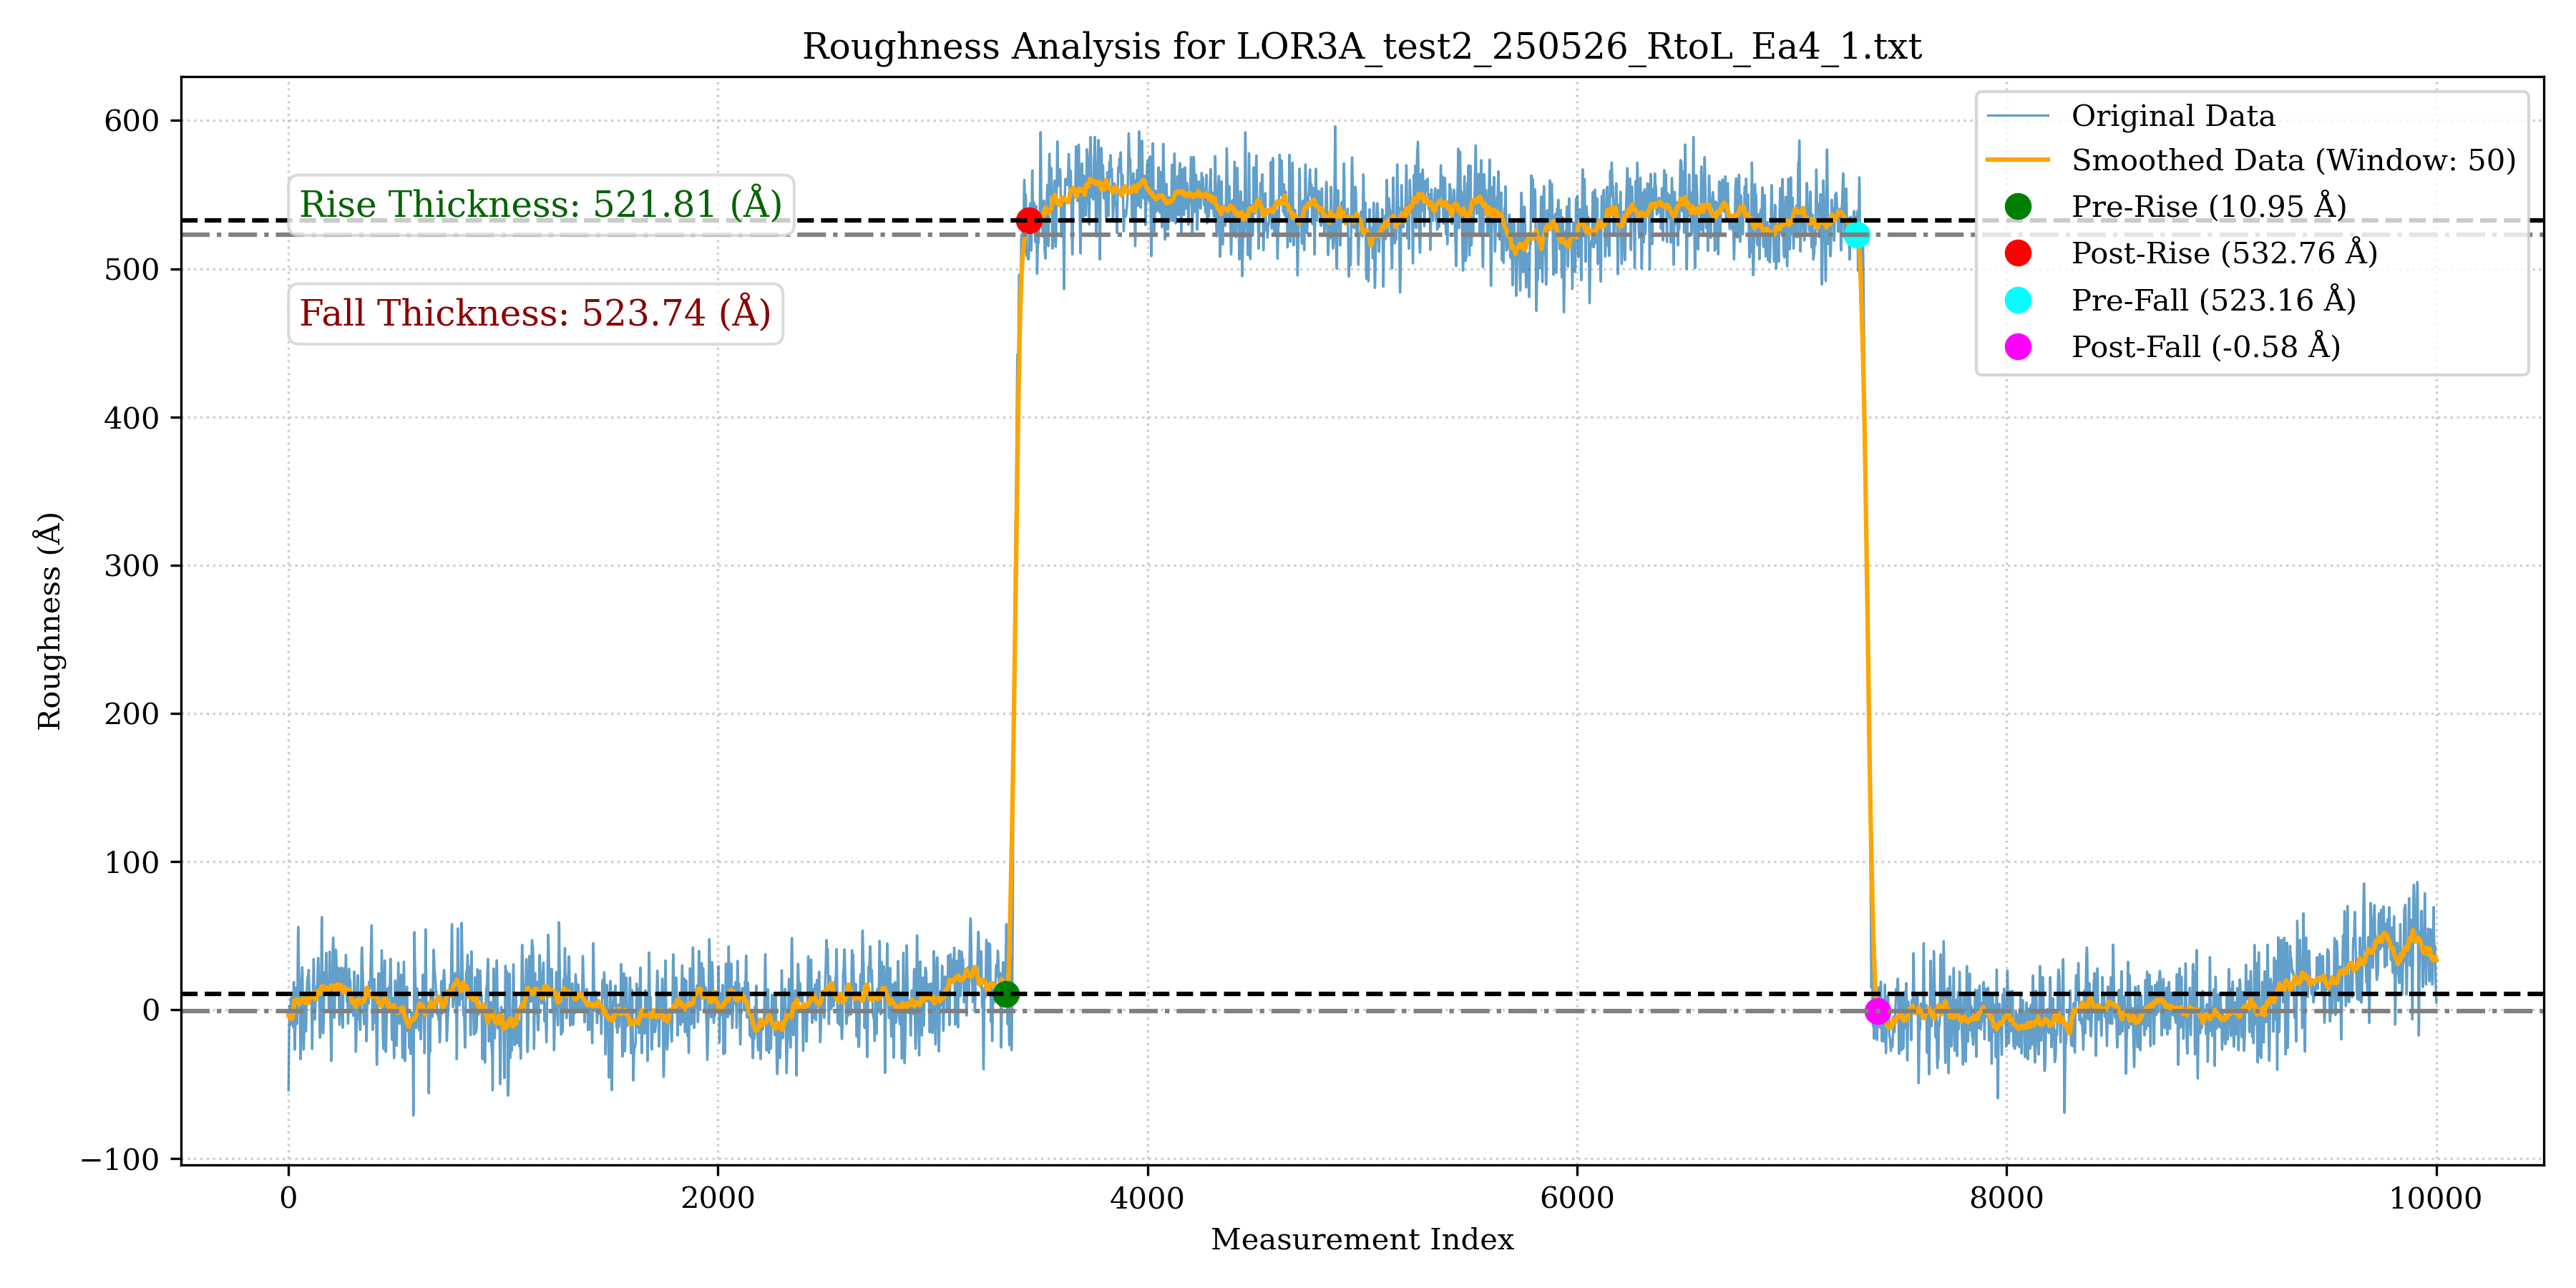
\includegraphics[width=\textwidth]{LOR3A_test2_250526_RtoL_Ea4_1.png}
    \label{fig:LOR3Atest2250526RtoLEa41}
\end{figure}
\begin{figure}[H]
    \centering
    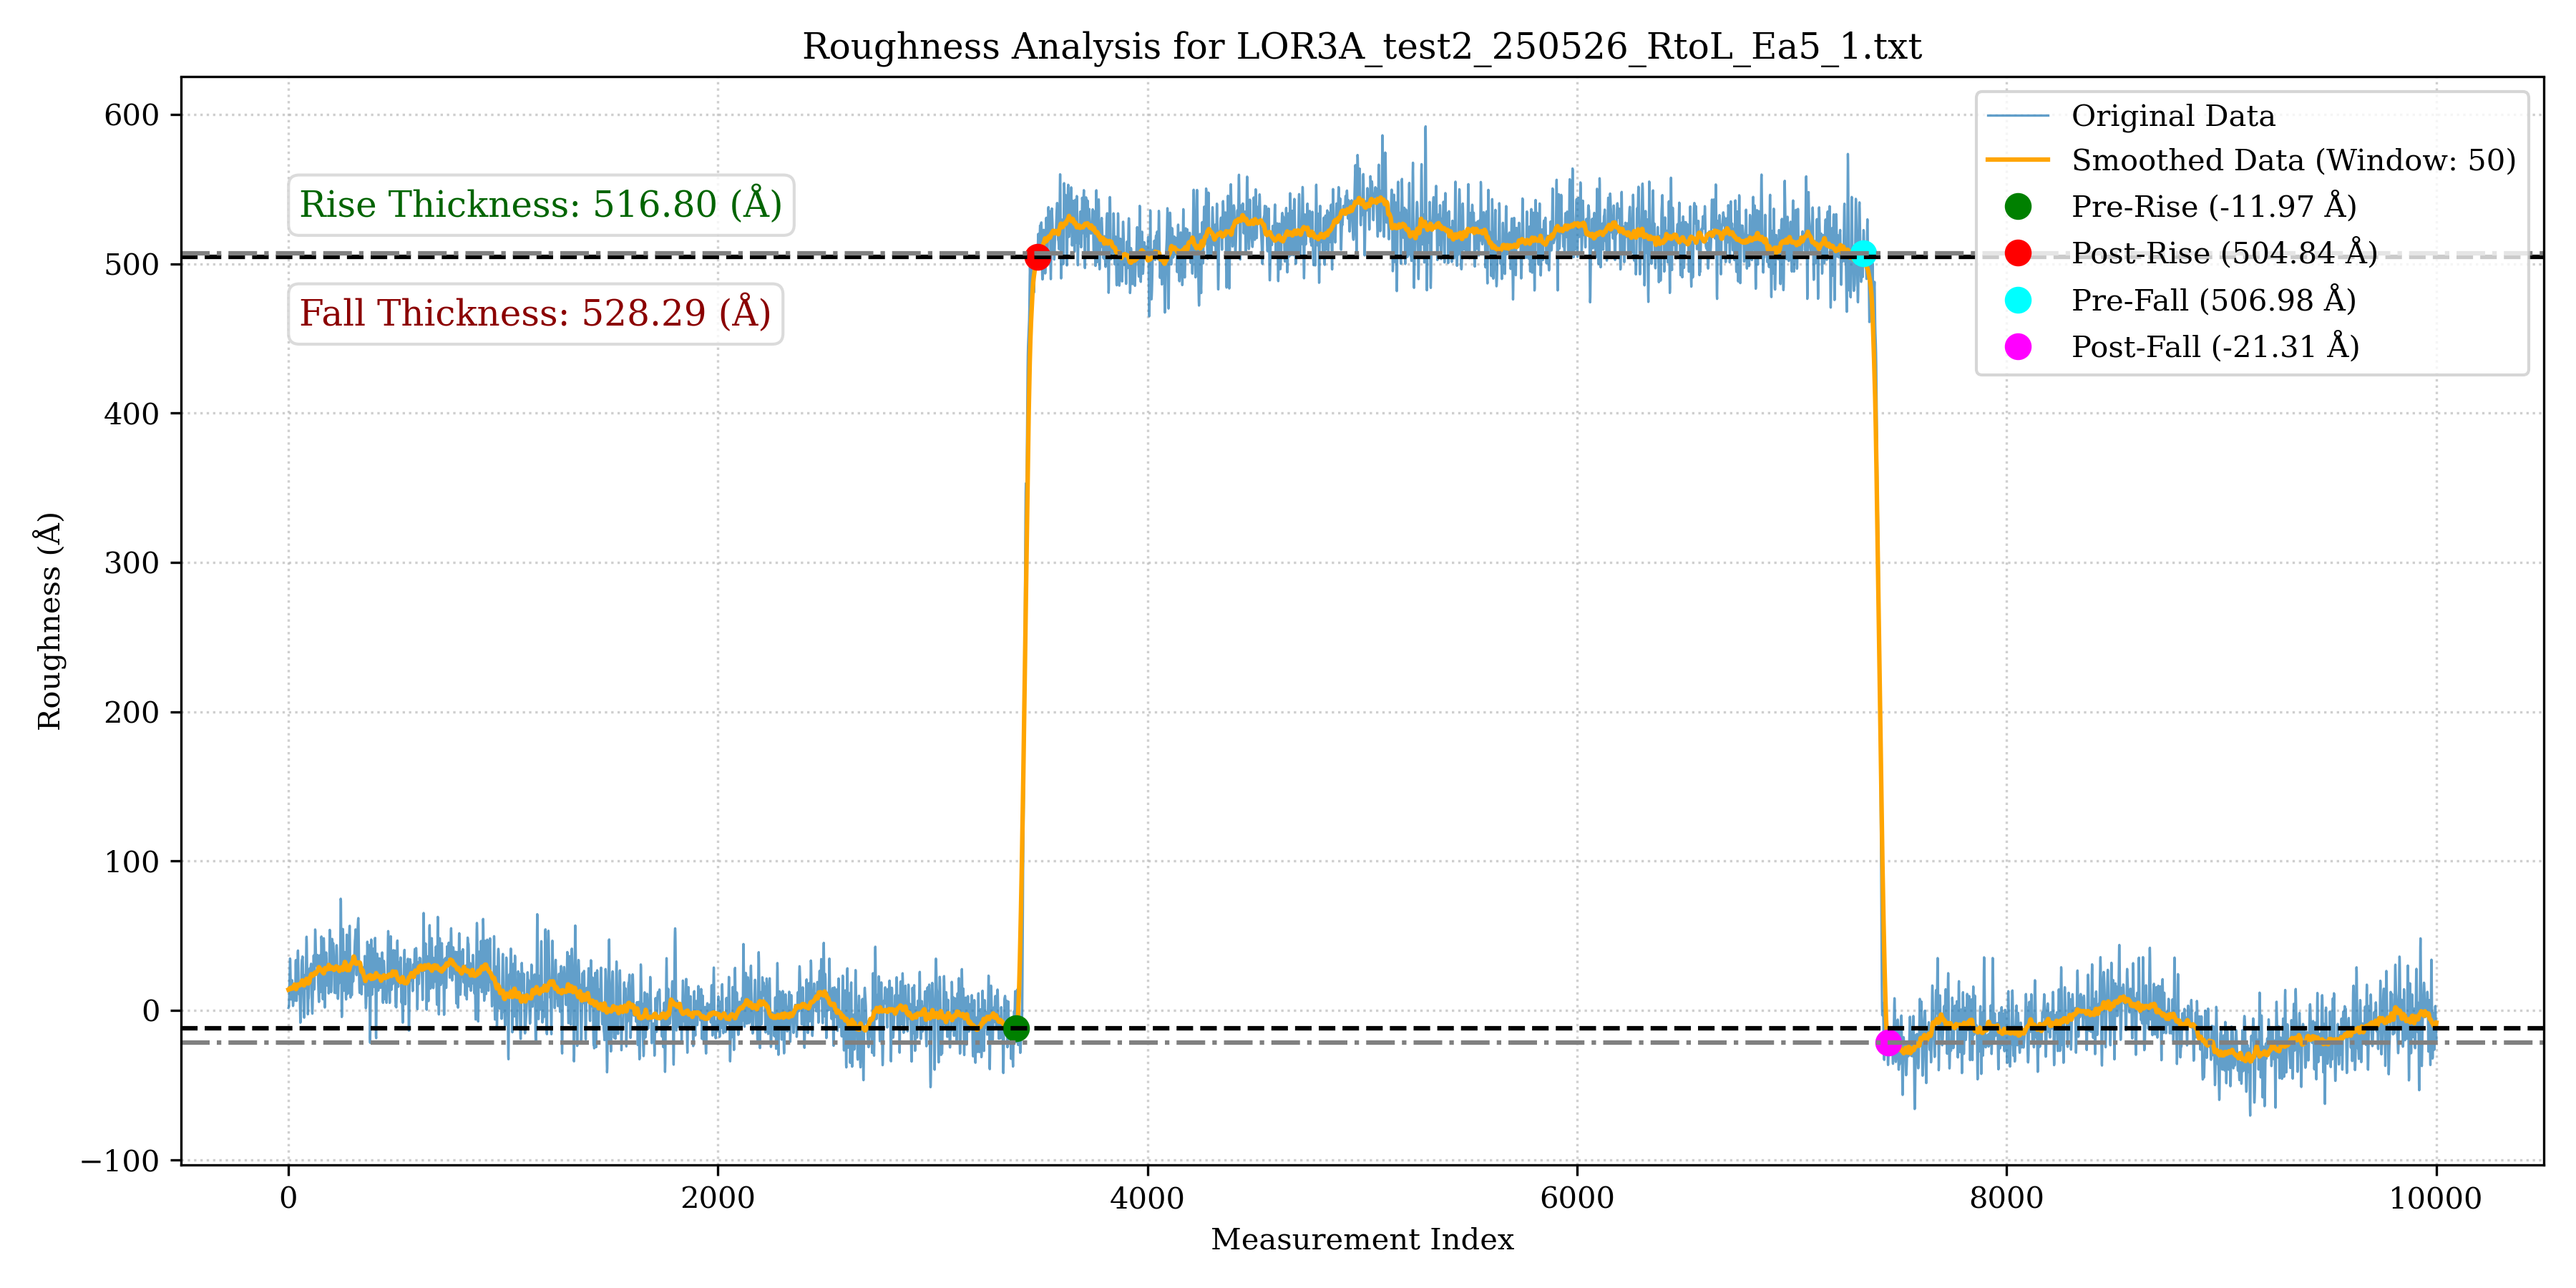
\includegraphics[width=\textwidth]{LOR3A_test2_250526_RtoL_Ea5_1.png}
    \label{fig:LOR3Atest2250526RtoLEa51}
\end{figure}
\begin{figure}[H]
    \centering
    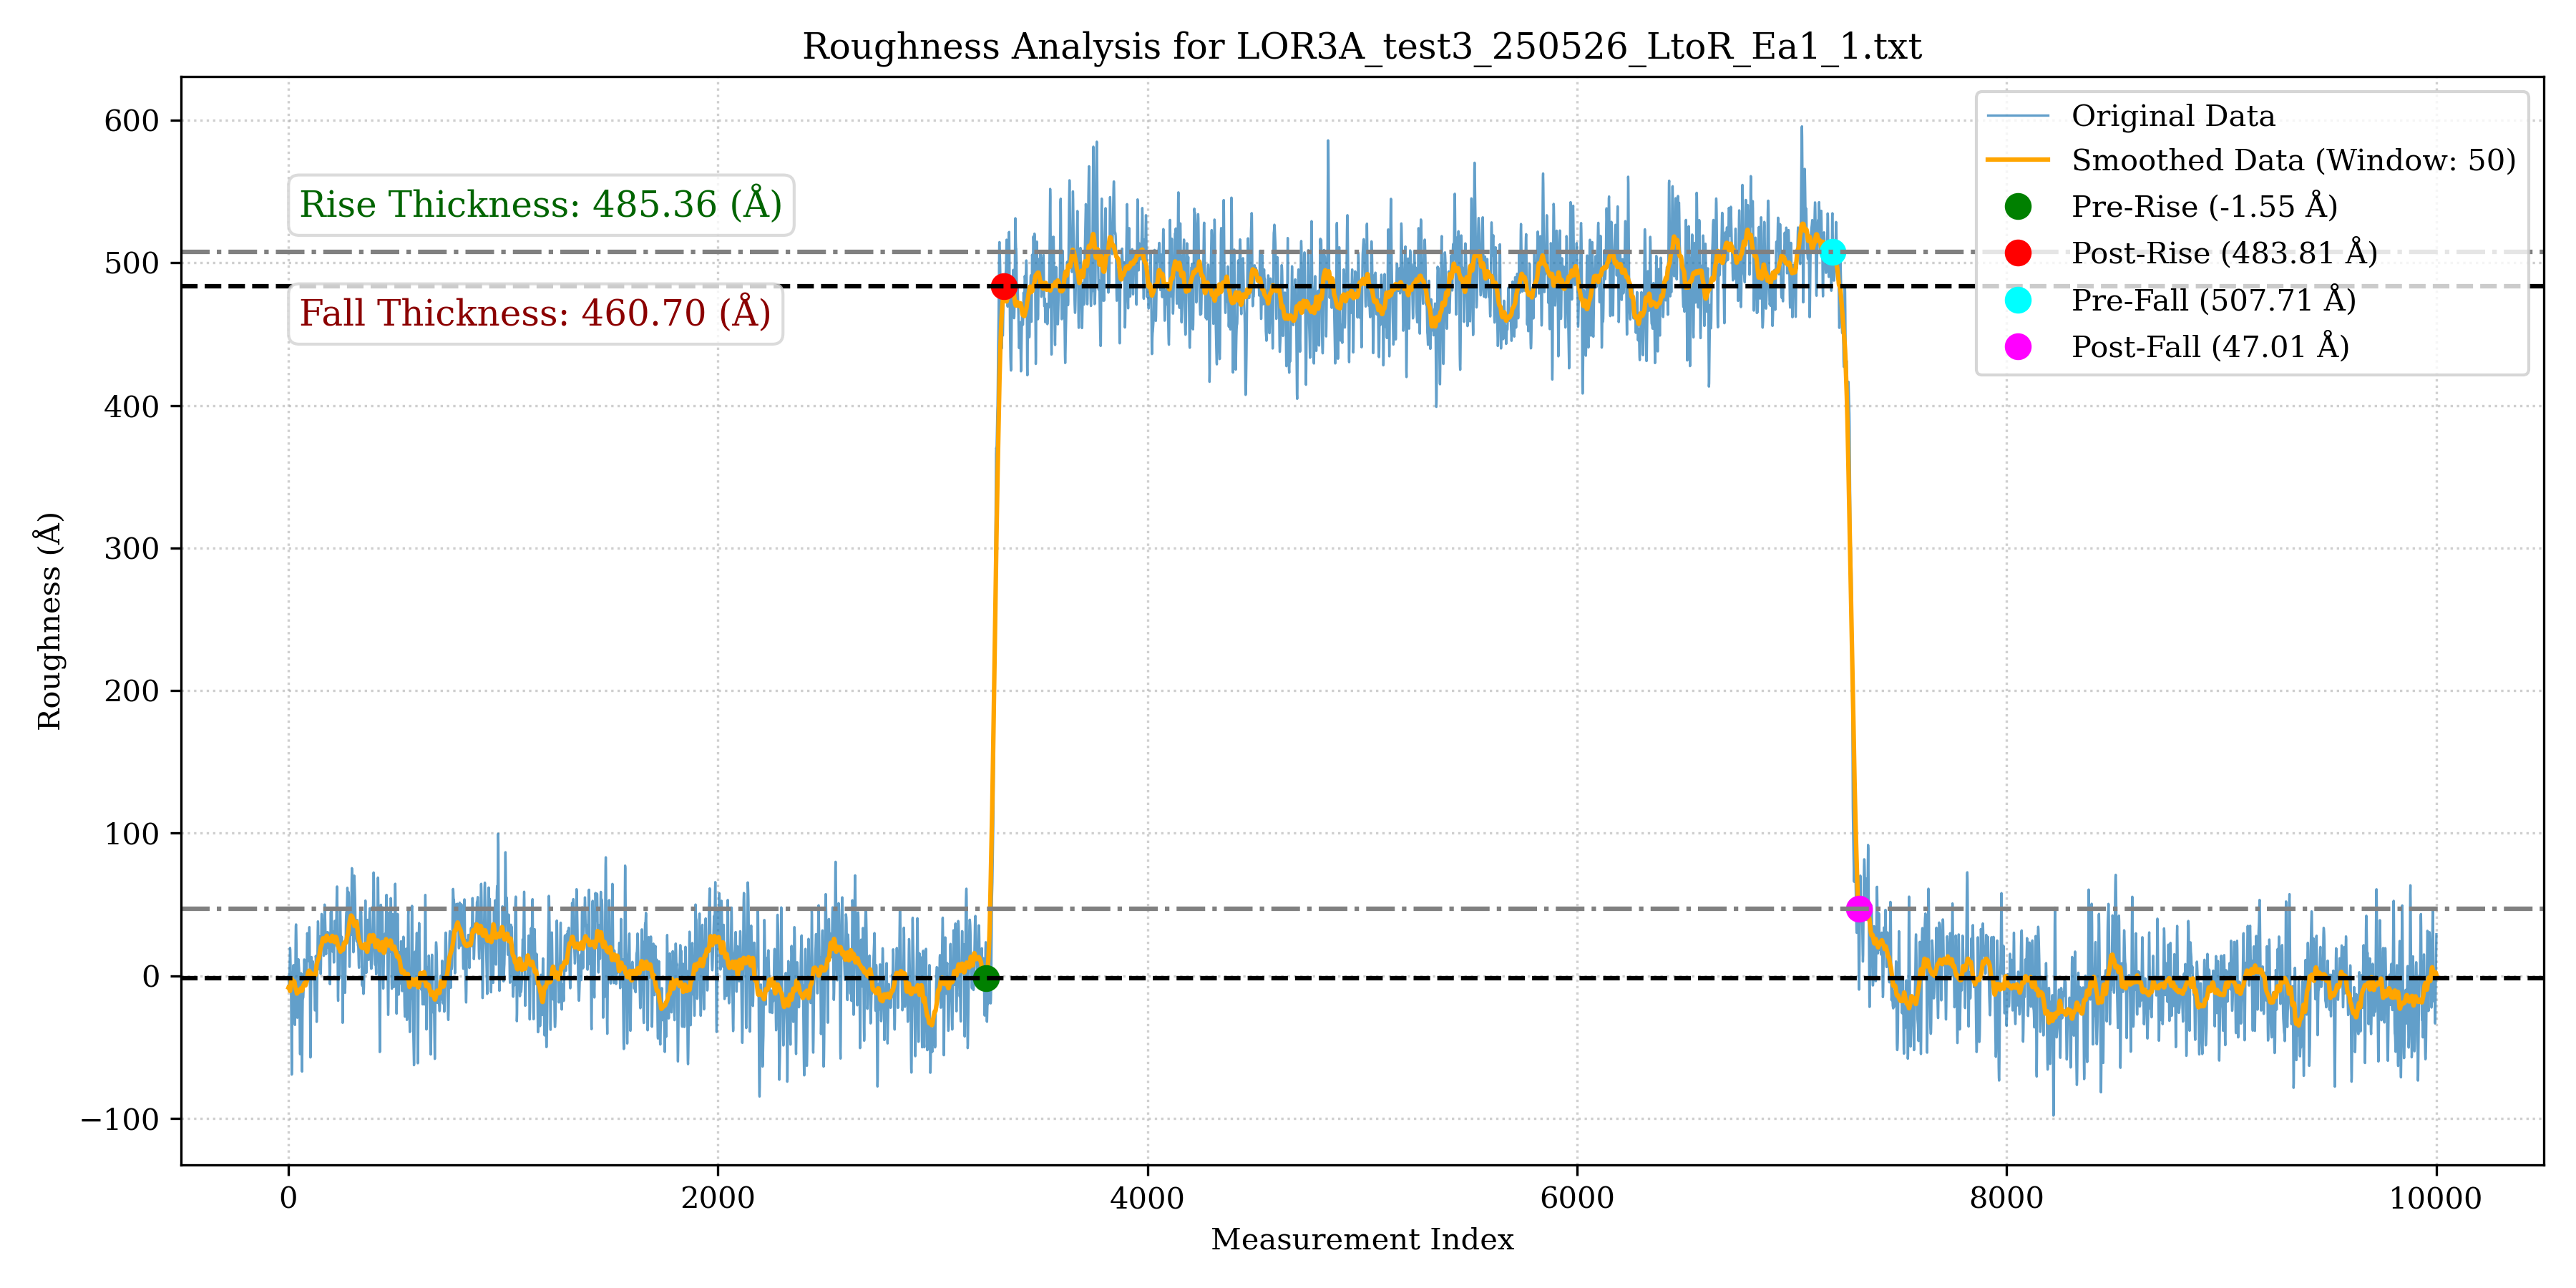
\includegraphics[width=\textwidth]{LOR3A_test3_250526_LtoR_Ea1_1.png}
    \label{fig:LOR3Atest3250526LtoREa11}
\end{figure}
\begin{figure}[H]
    \centering
    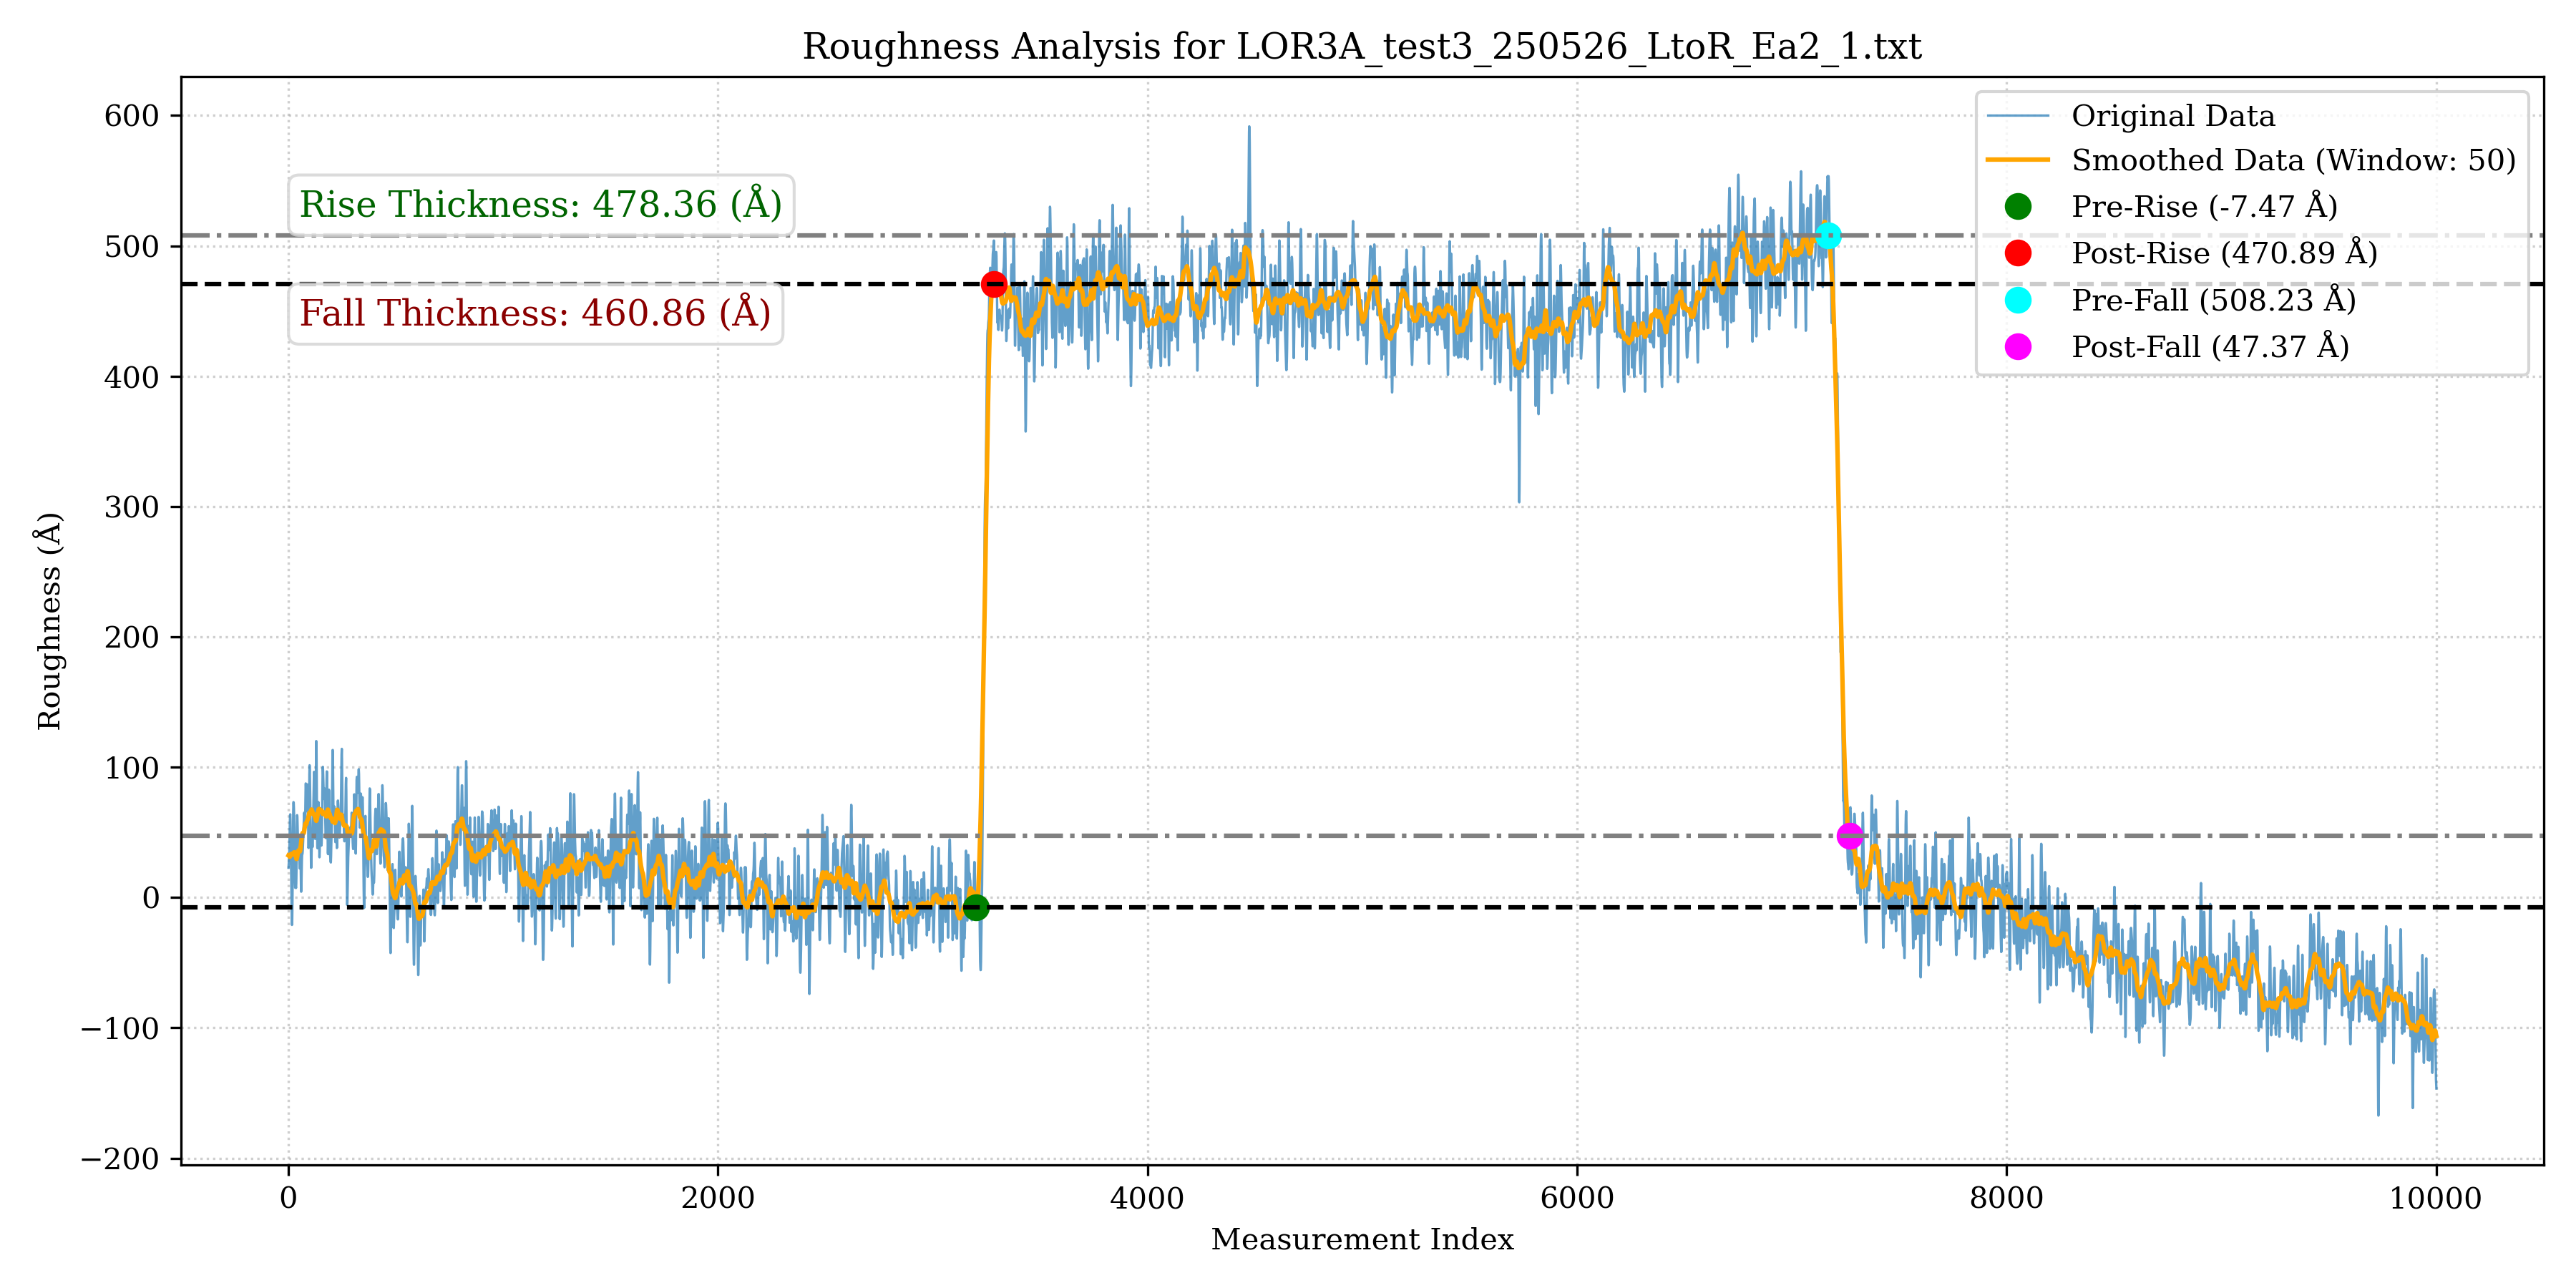
\includegraphics[width=\textwidth]{LOR3A_test3_250526_LtoR_Ea2_1.png}
    \label{fig:LOR3Atest3250526LtoREa21}
\end{figure}
\begin{figure}[H]
    \centering
    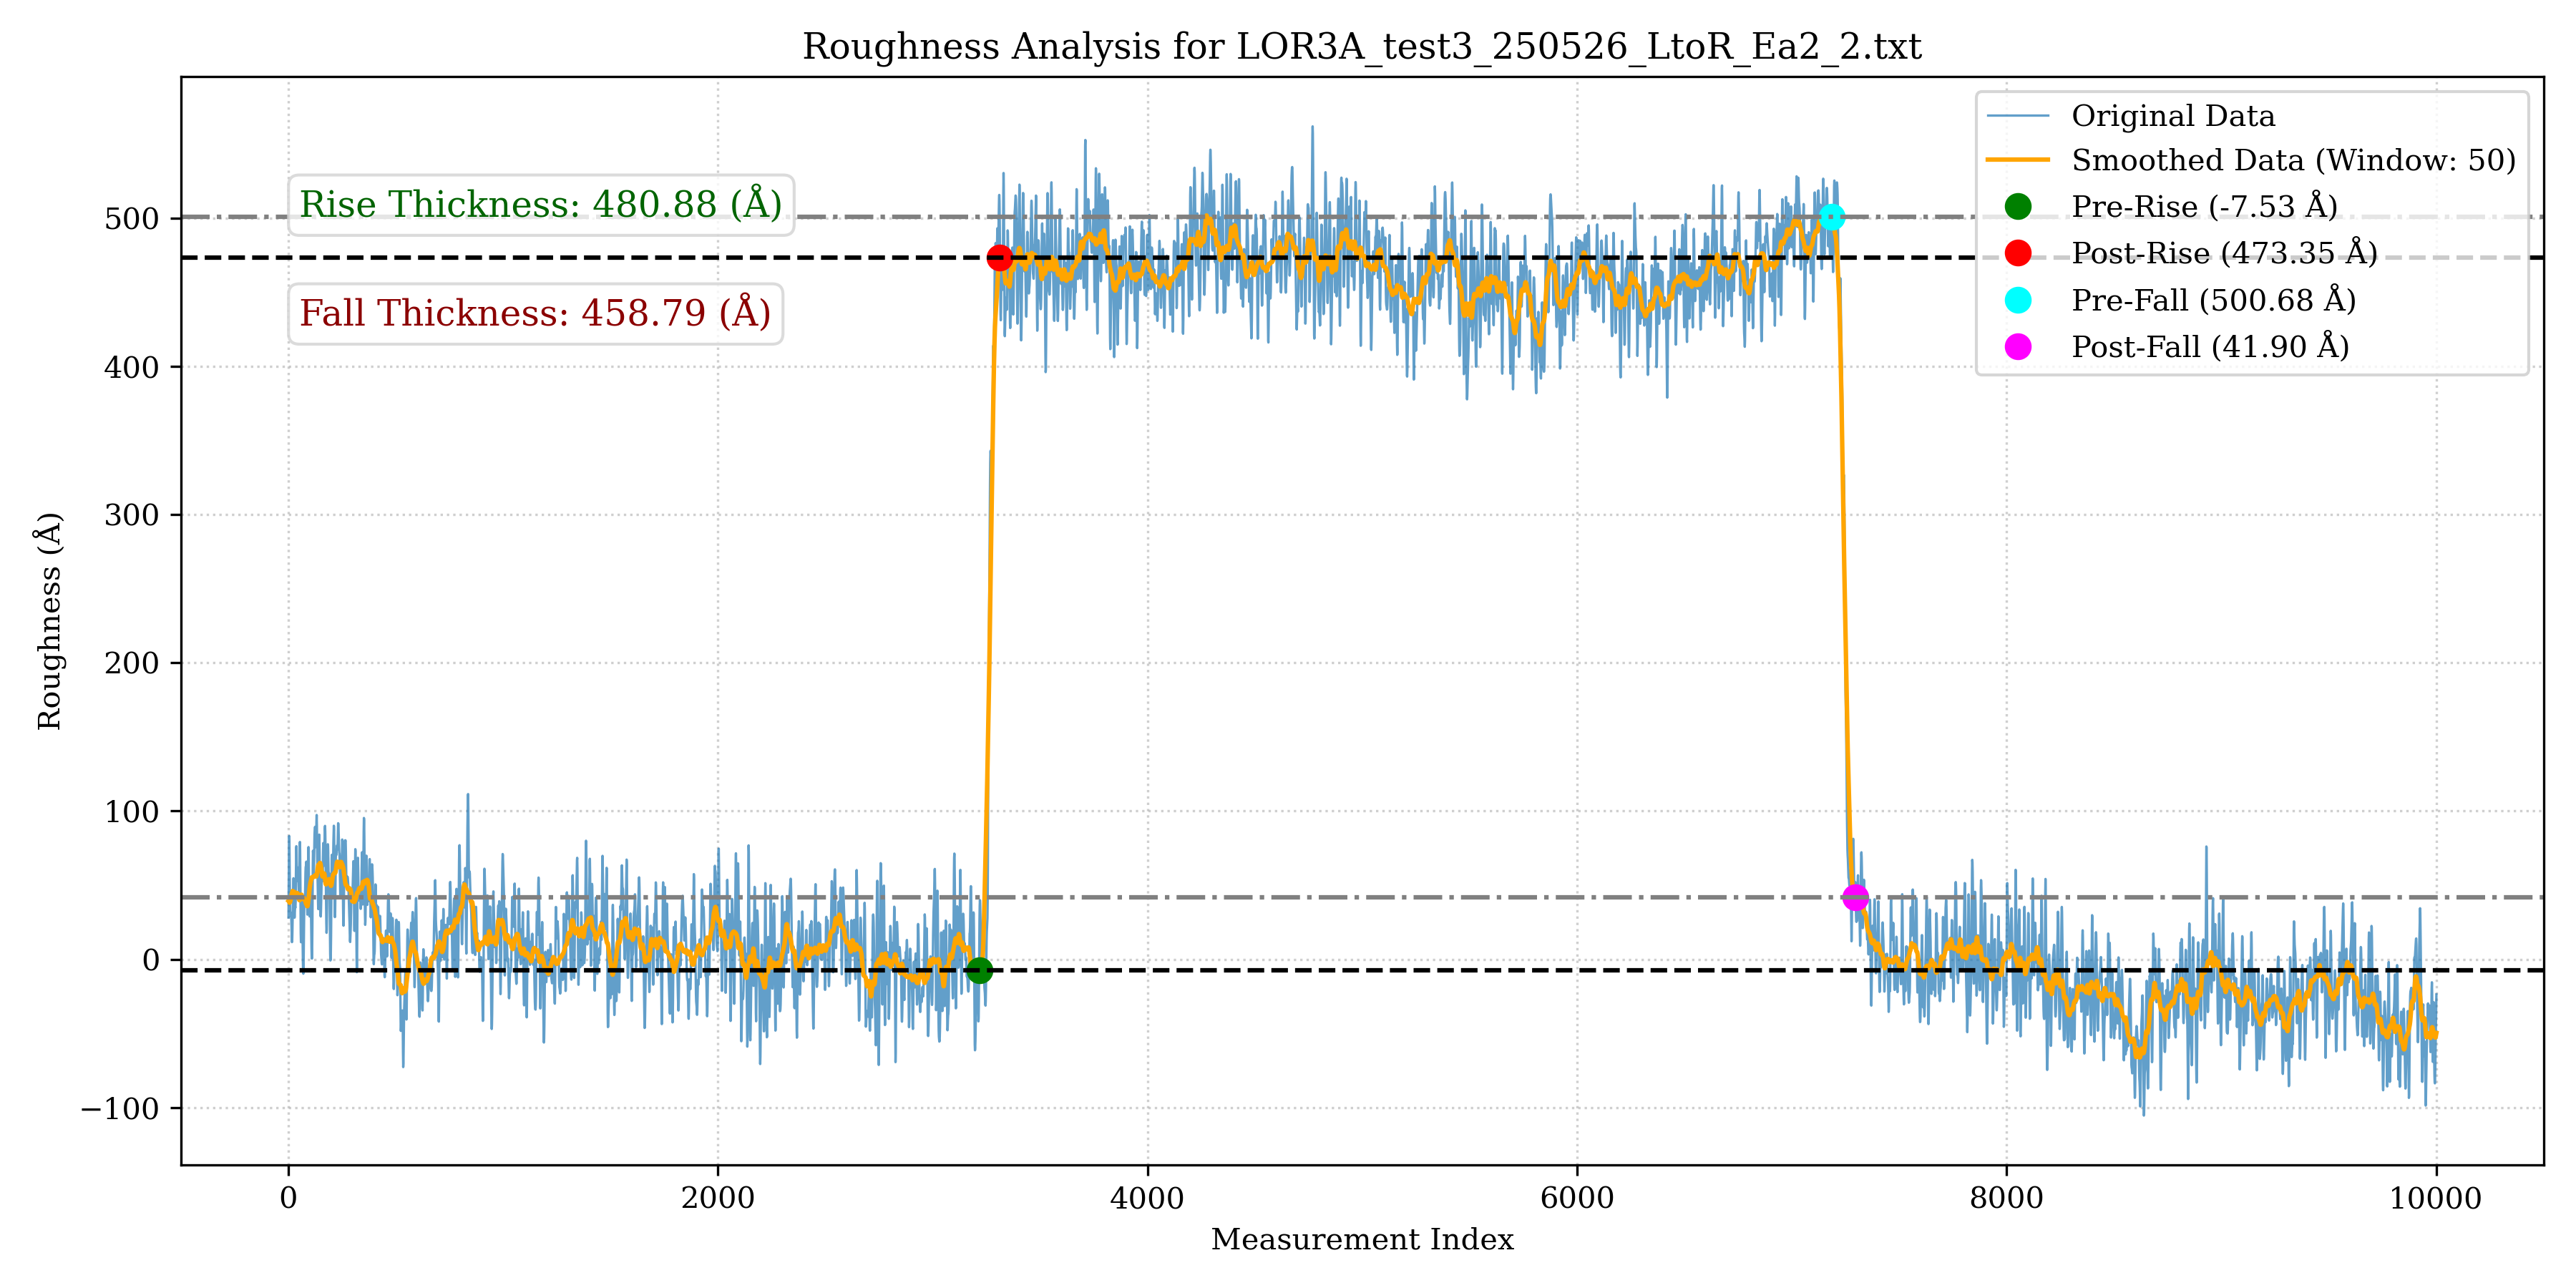
\includegraphics[width=\textwidth]{LOR3A_test3_250526_LtoR_Ea2_2.png}
    \label{fig:LOR3Atest3250526LtoREa22}
\end{figure}
\begin{figure}[H]
    \centering
    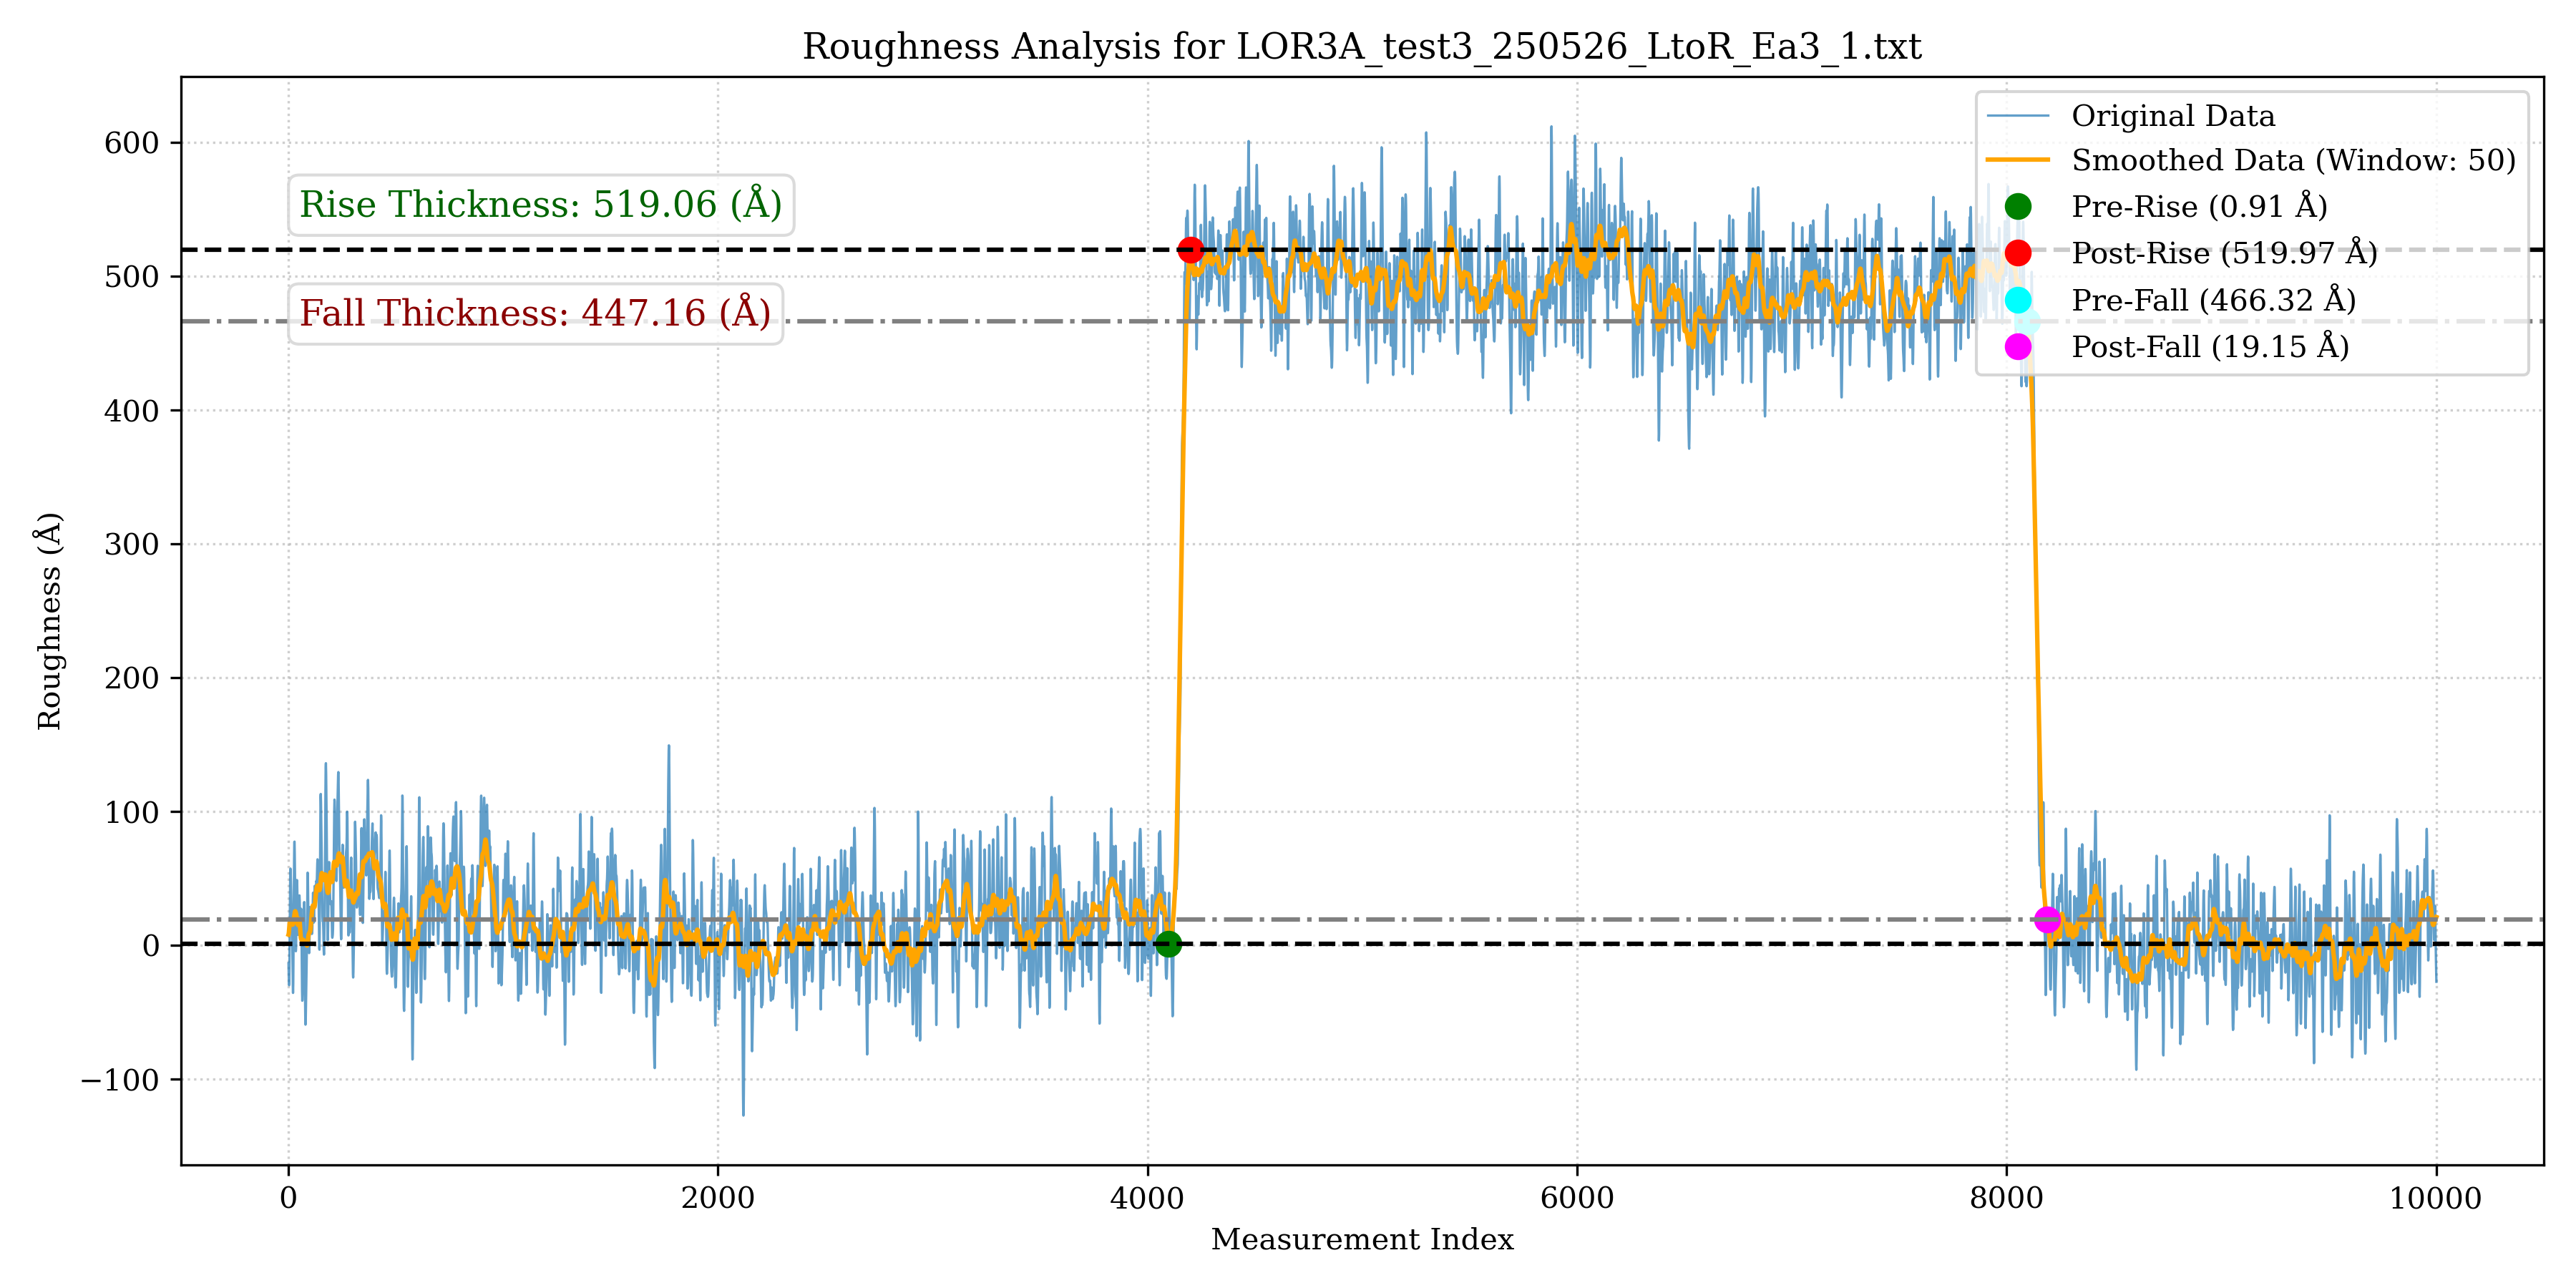
\includegraphics[width=\textwidth]{LOR3A_test3_250526_LtoR_Ea3_1.png}
    \label{fig:LOR3Atest3250526LtoREa31}
\end{figure}
\begin{figure}[H]
    \centering
    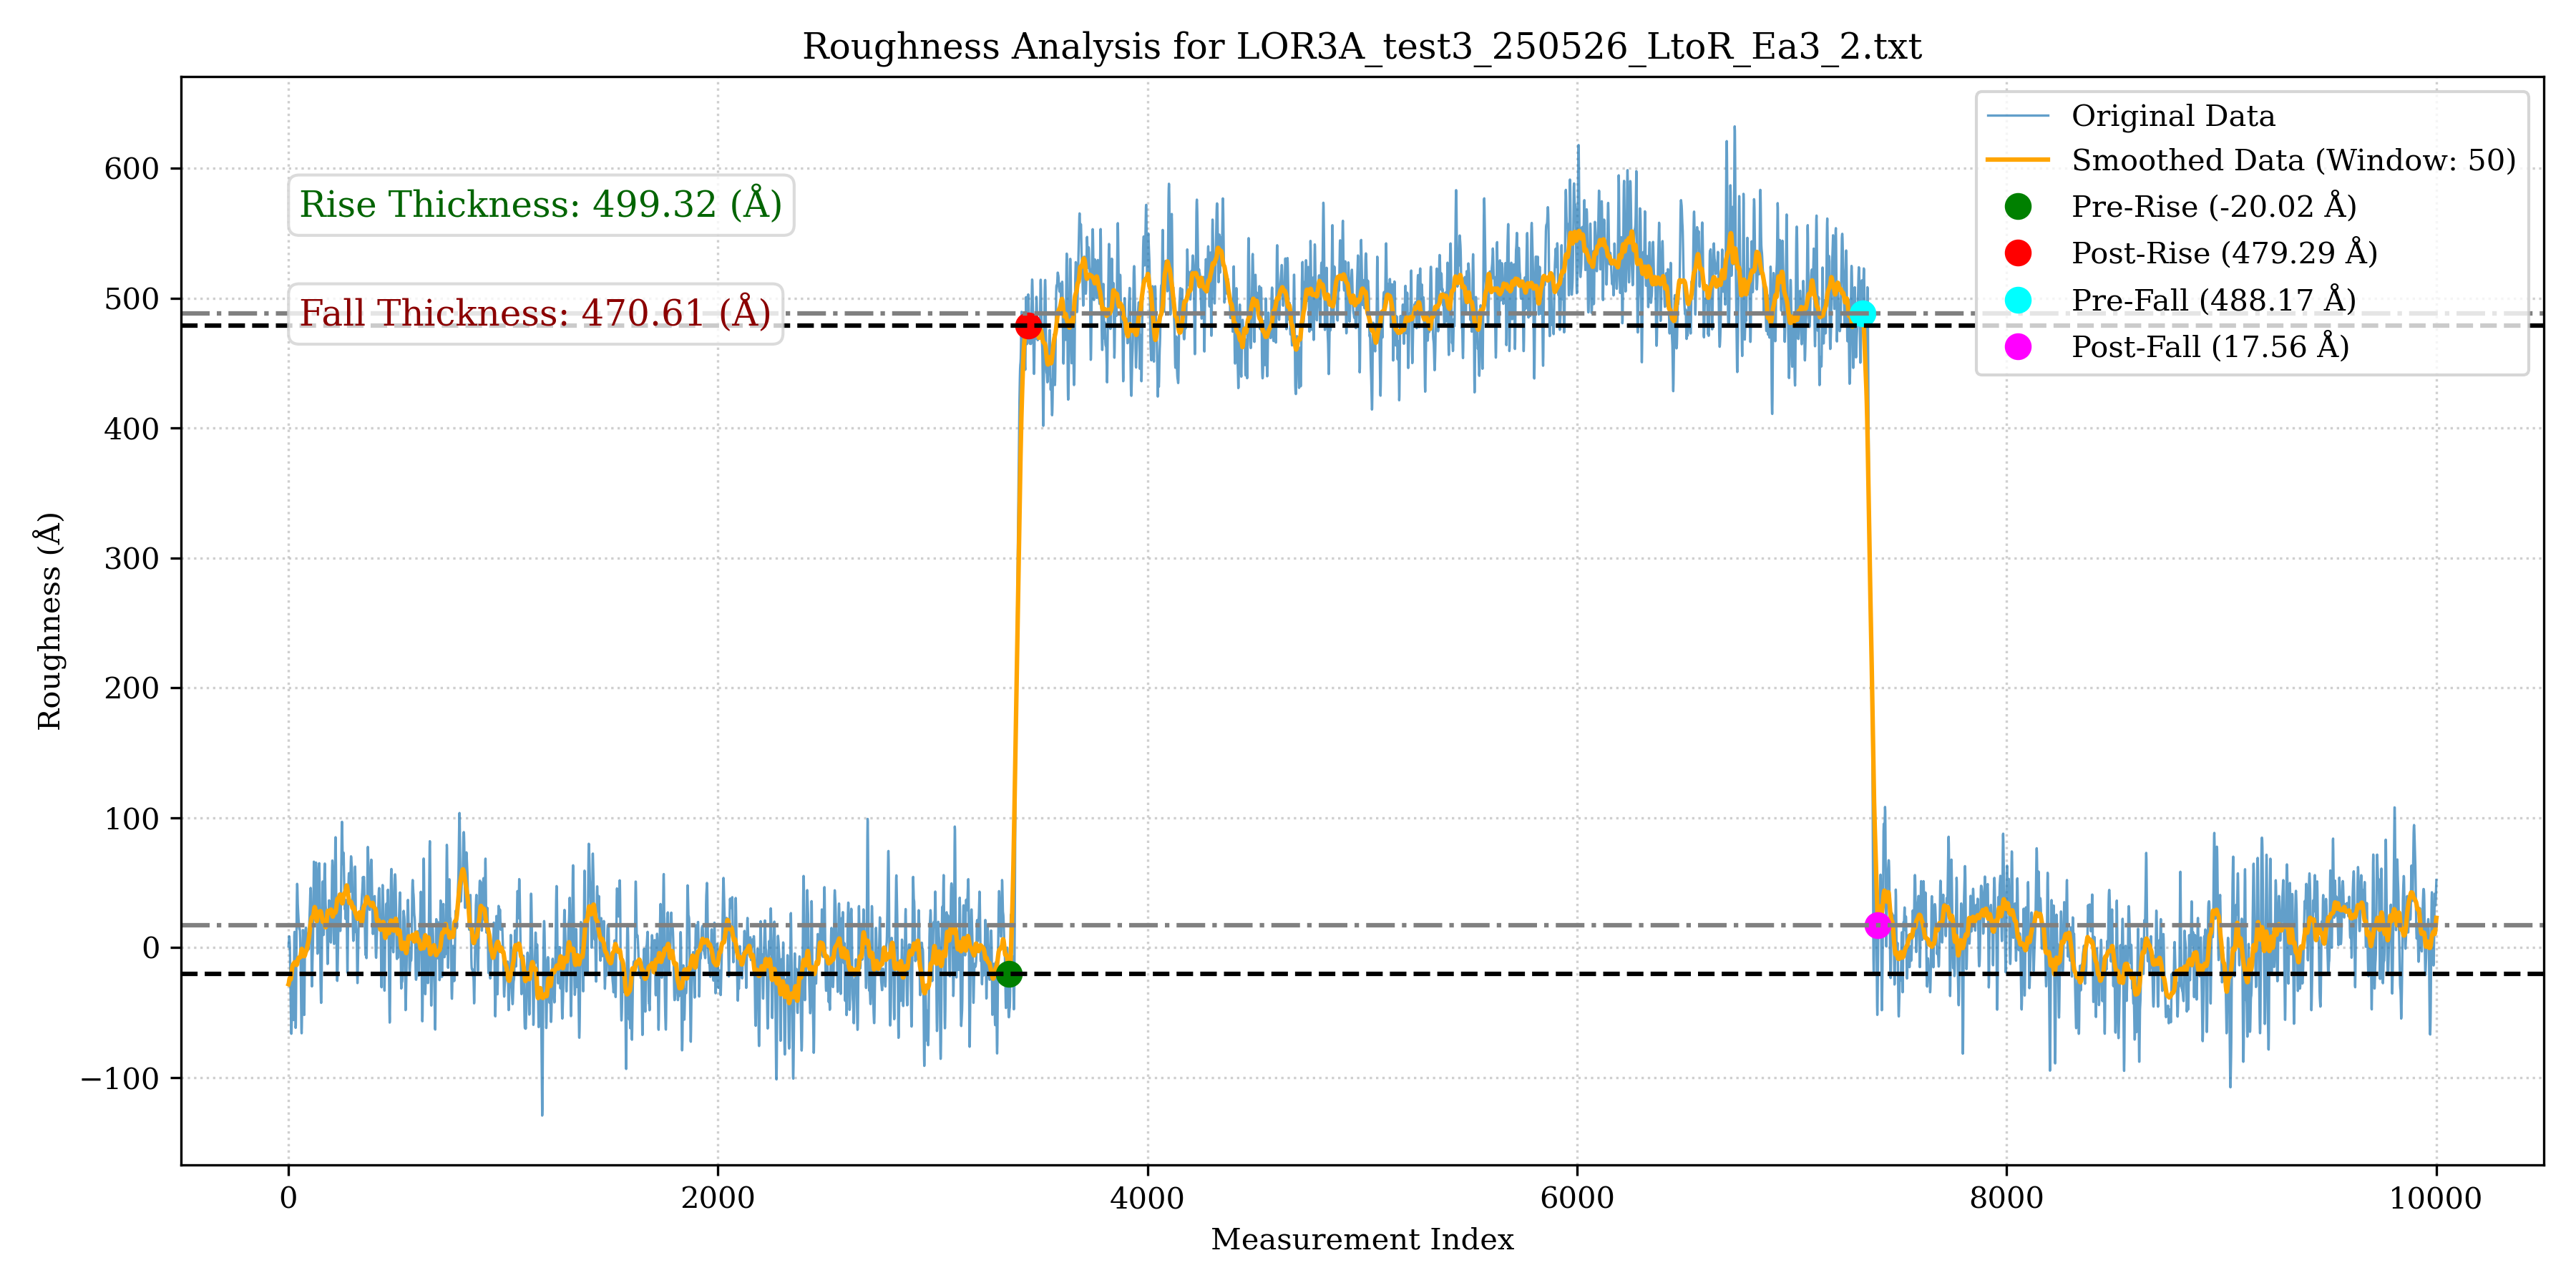
\includegraphics[width=\textwidth]{LOR3A_test3_250526_LtoR_Ea3_2.png}
    \label{fig:LOR3Atest3250526LtoREa32}
\end{figure}
\begin{figure}[H]
    \centering
    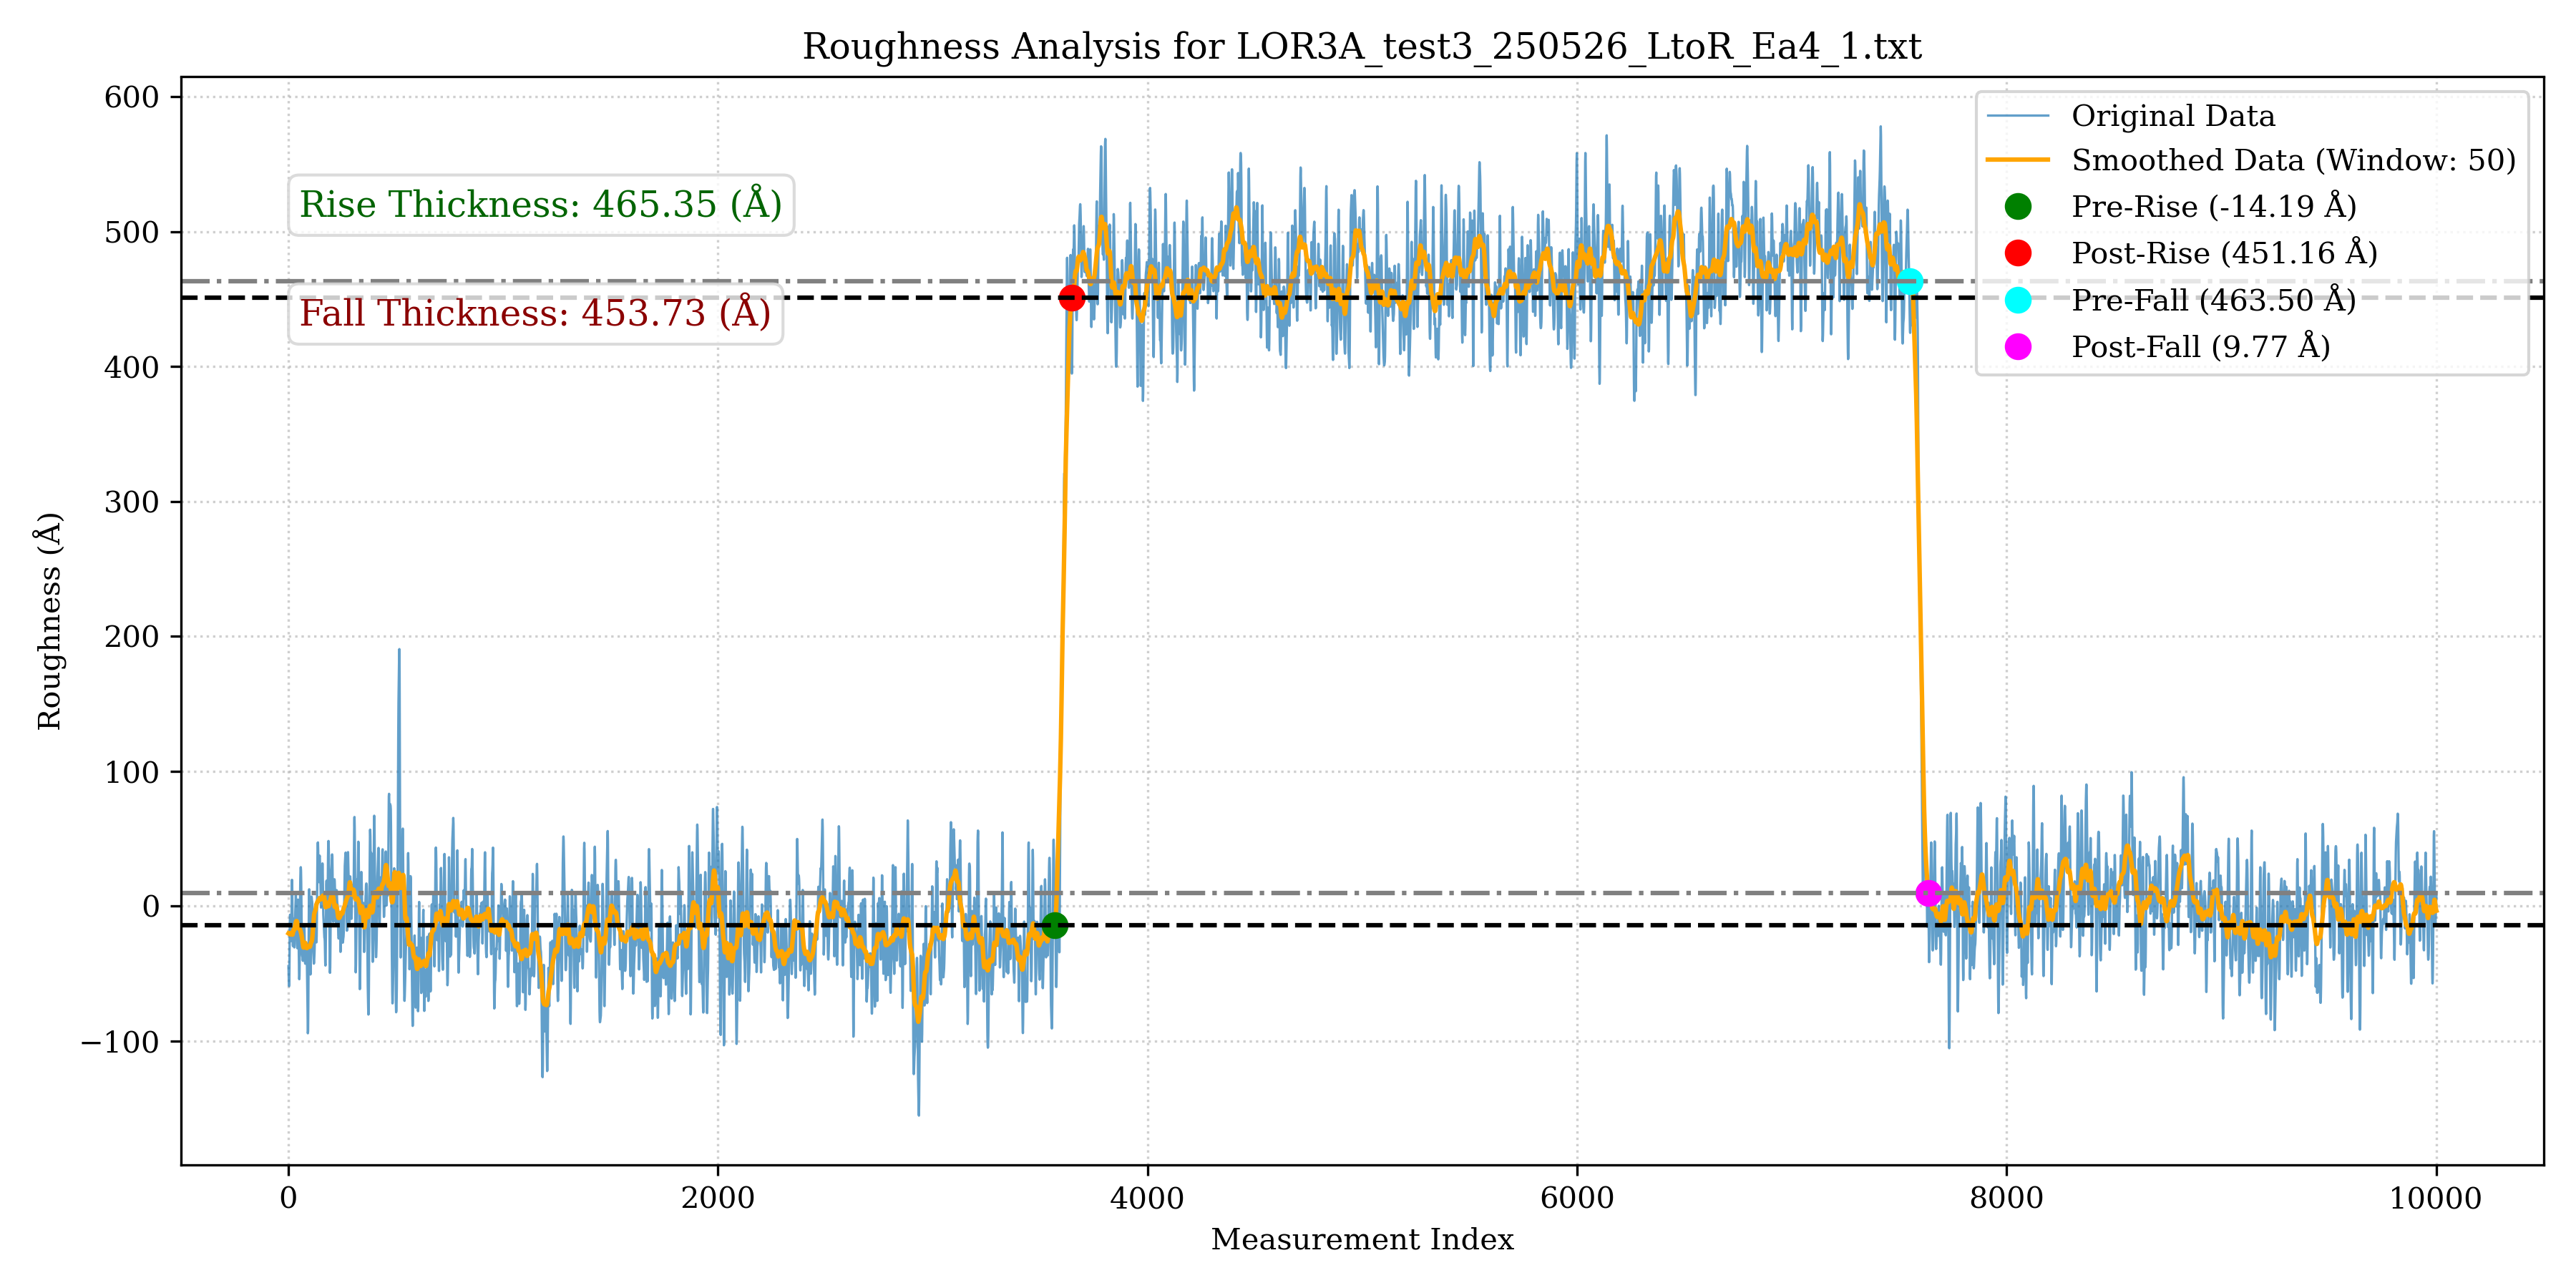
\includegraphics[width=\textwidth]{LOR3A_test3_250526_LtoR_Ea4_1.png}
    \label{fig:LOR3Atest3250526LtoREa41}
\end{figure}
\begin{figure}[H]
    \centering
    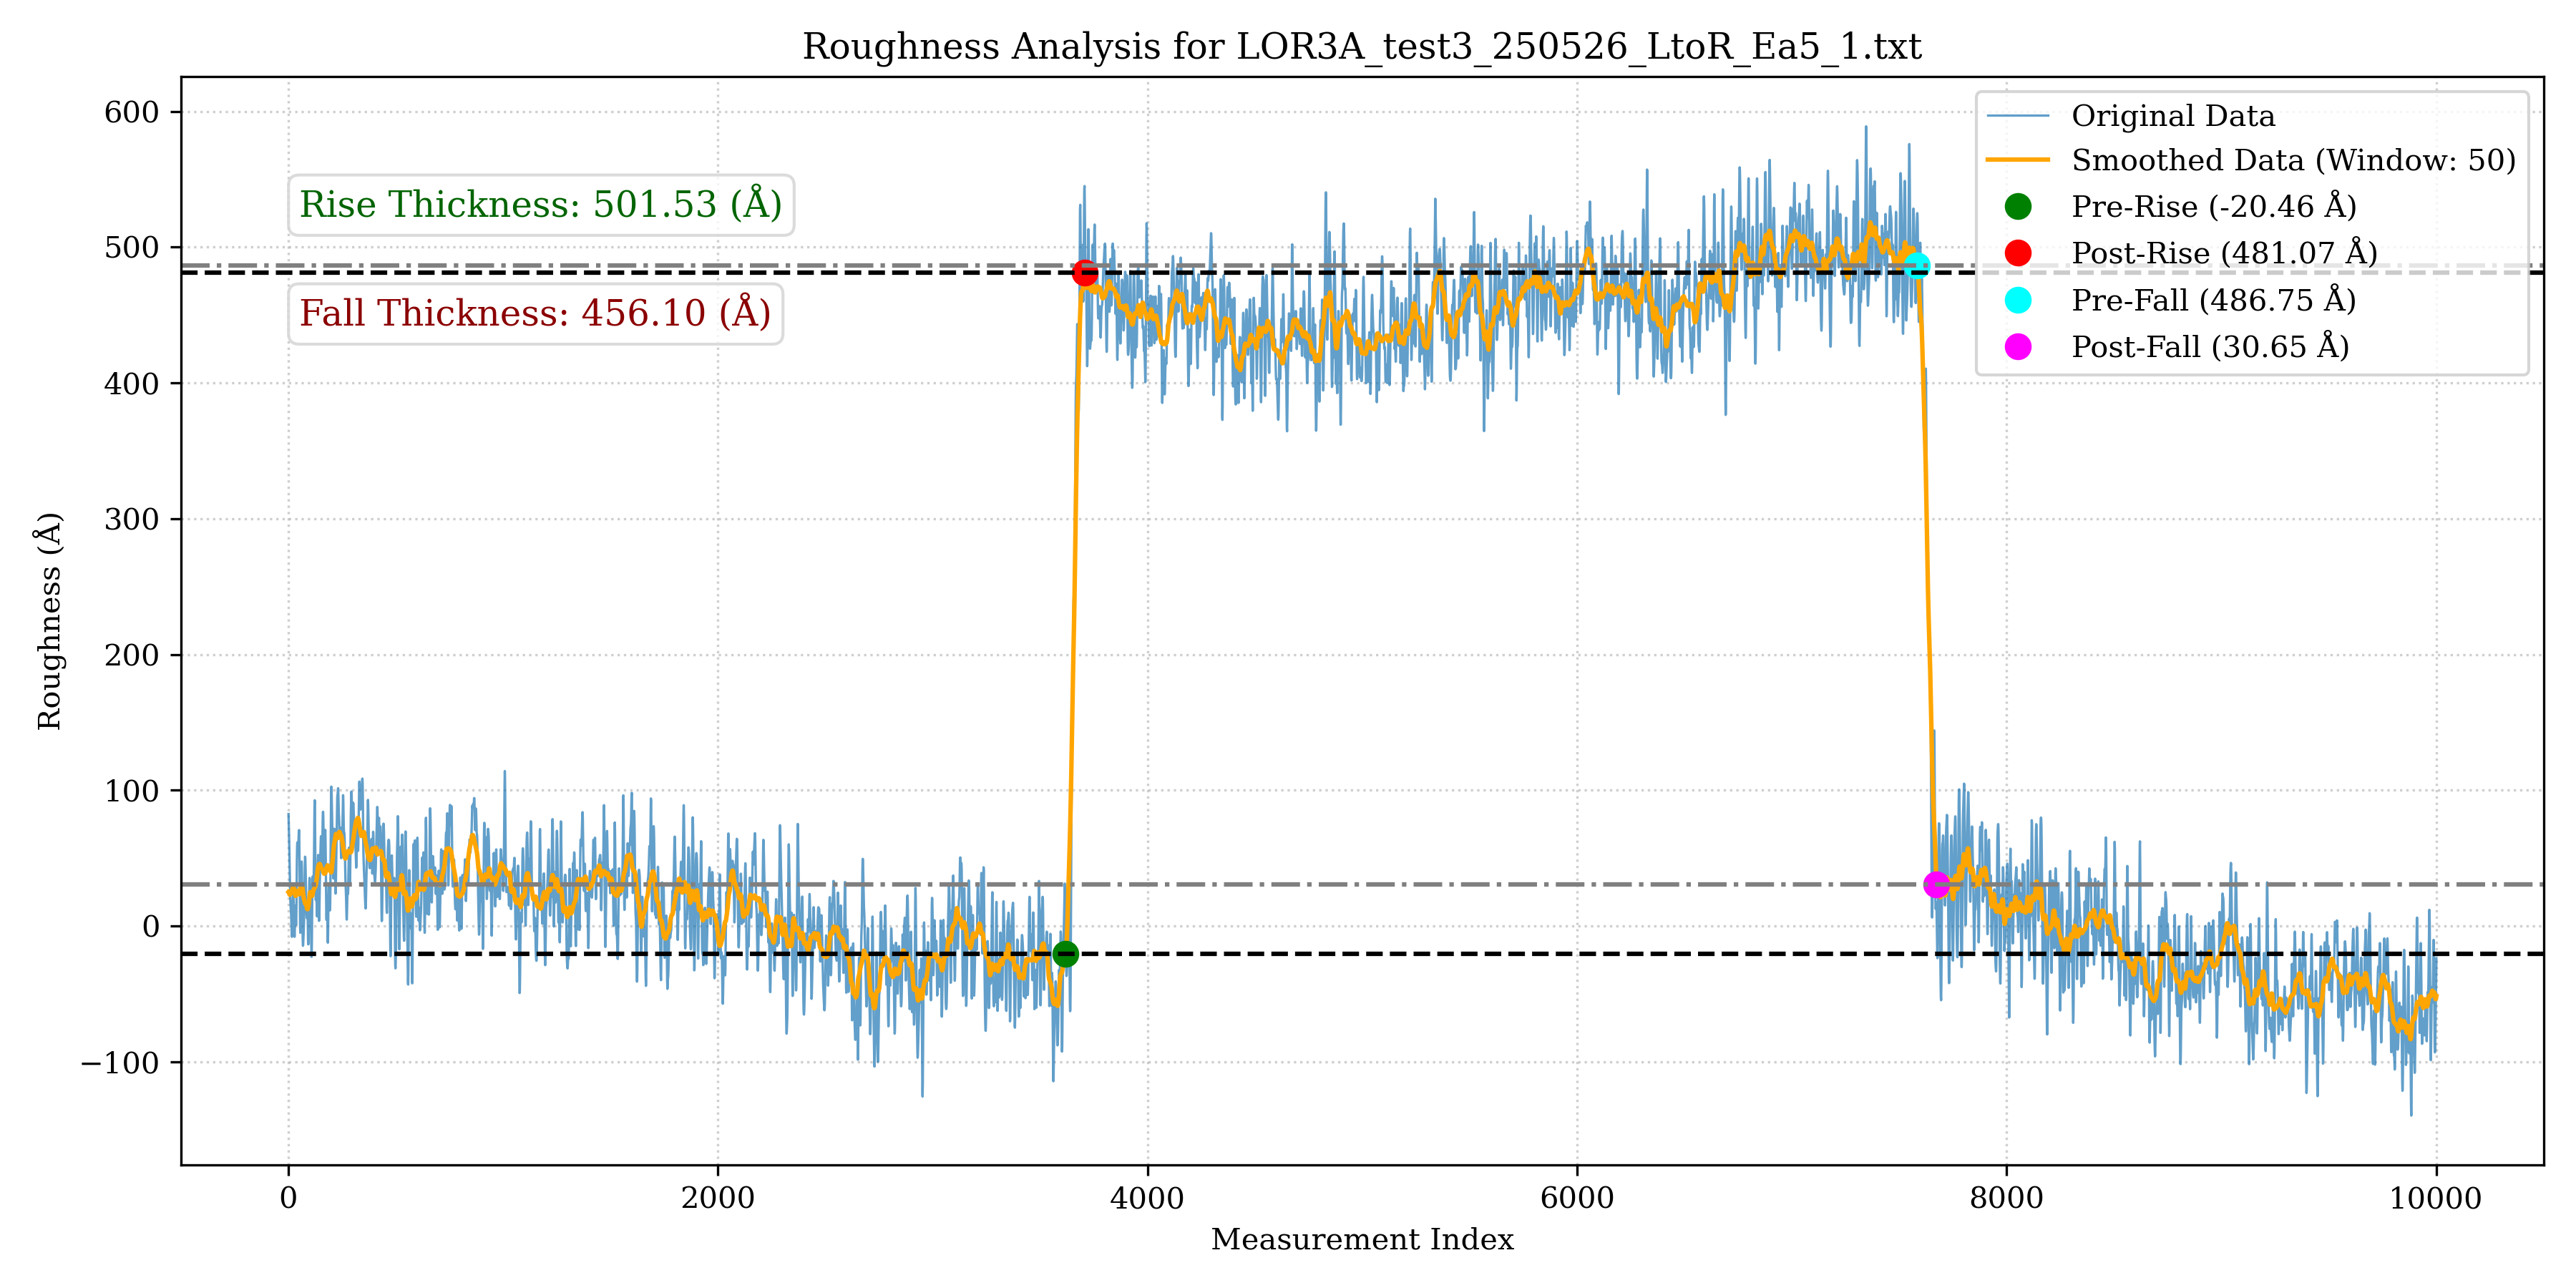
\includegraphics[width=\textwidth]{LOR3A_test3_250526_LtoR_Ea5_1.png}
    \label{fig:LOR3Atest3250526LtoREa51}
\end{figure}
\begin{figure}[H]
    \centering
    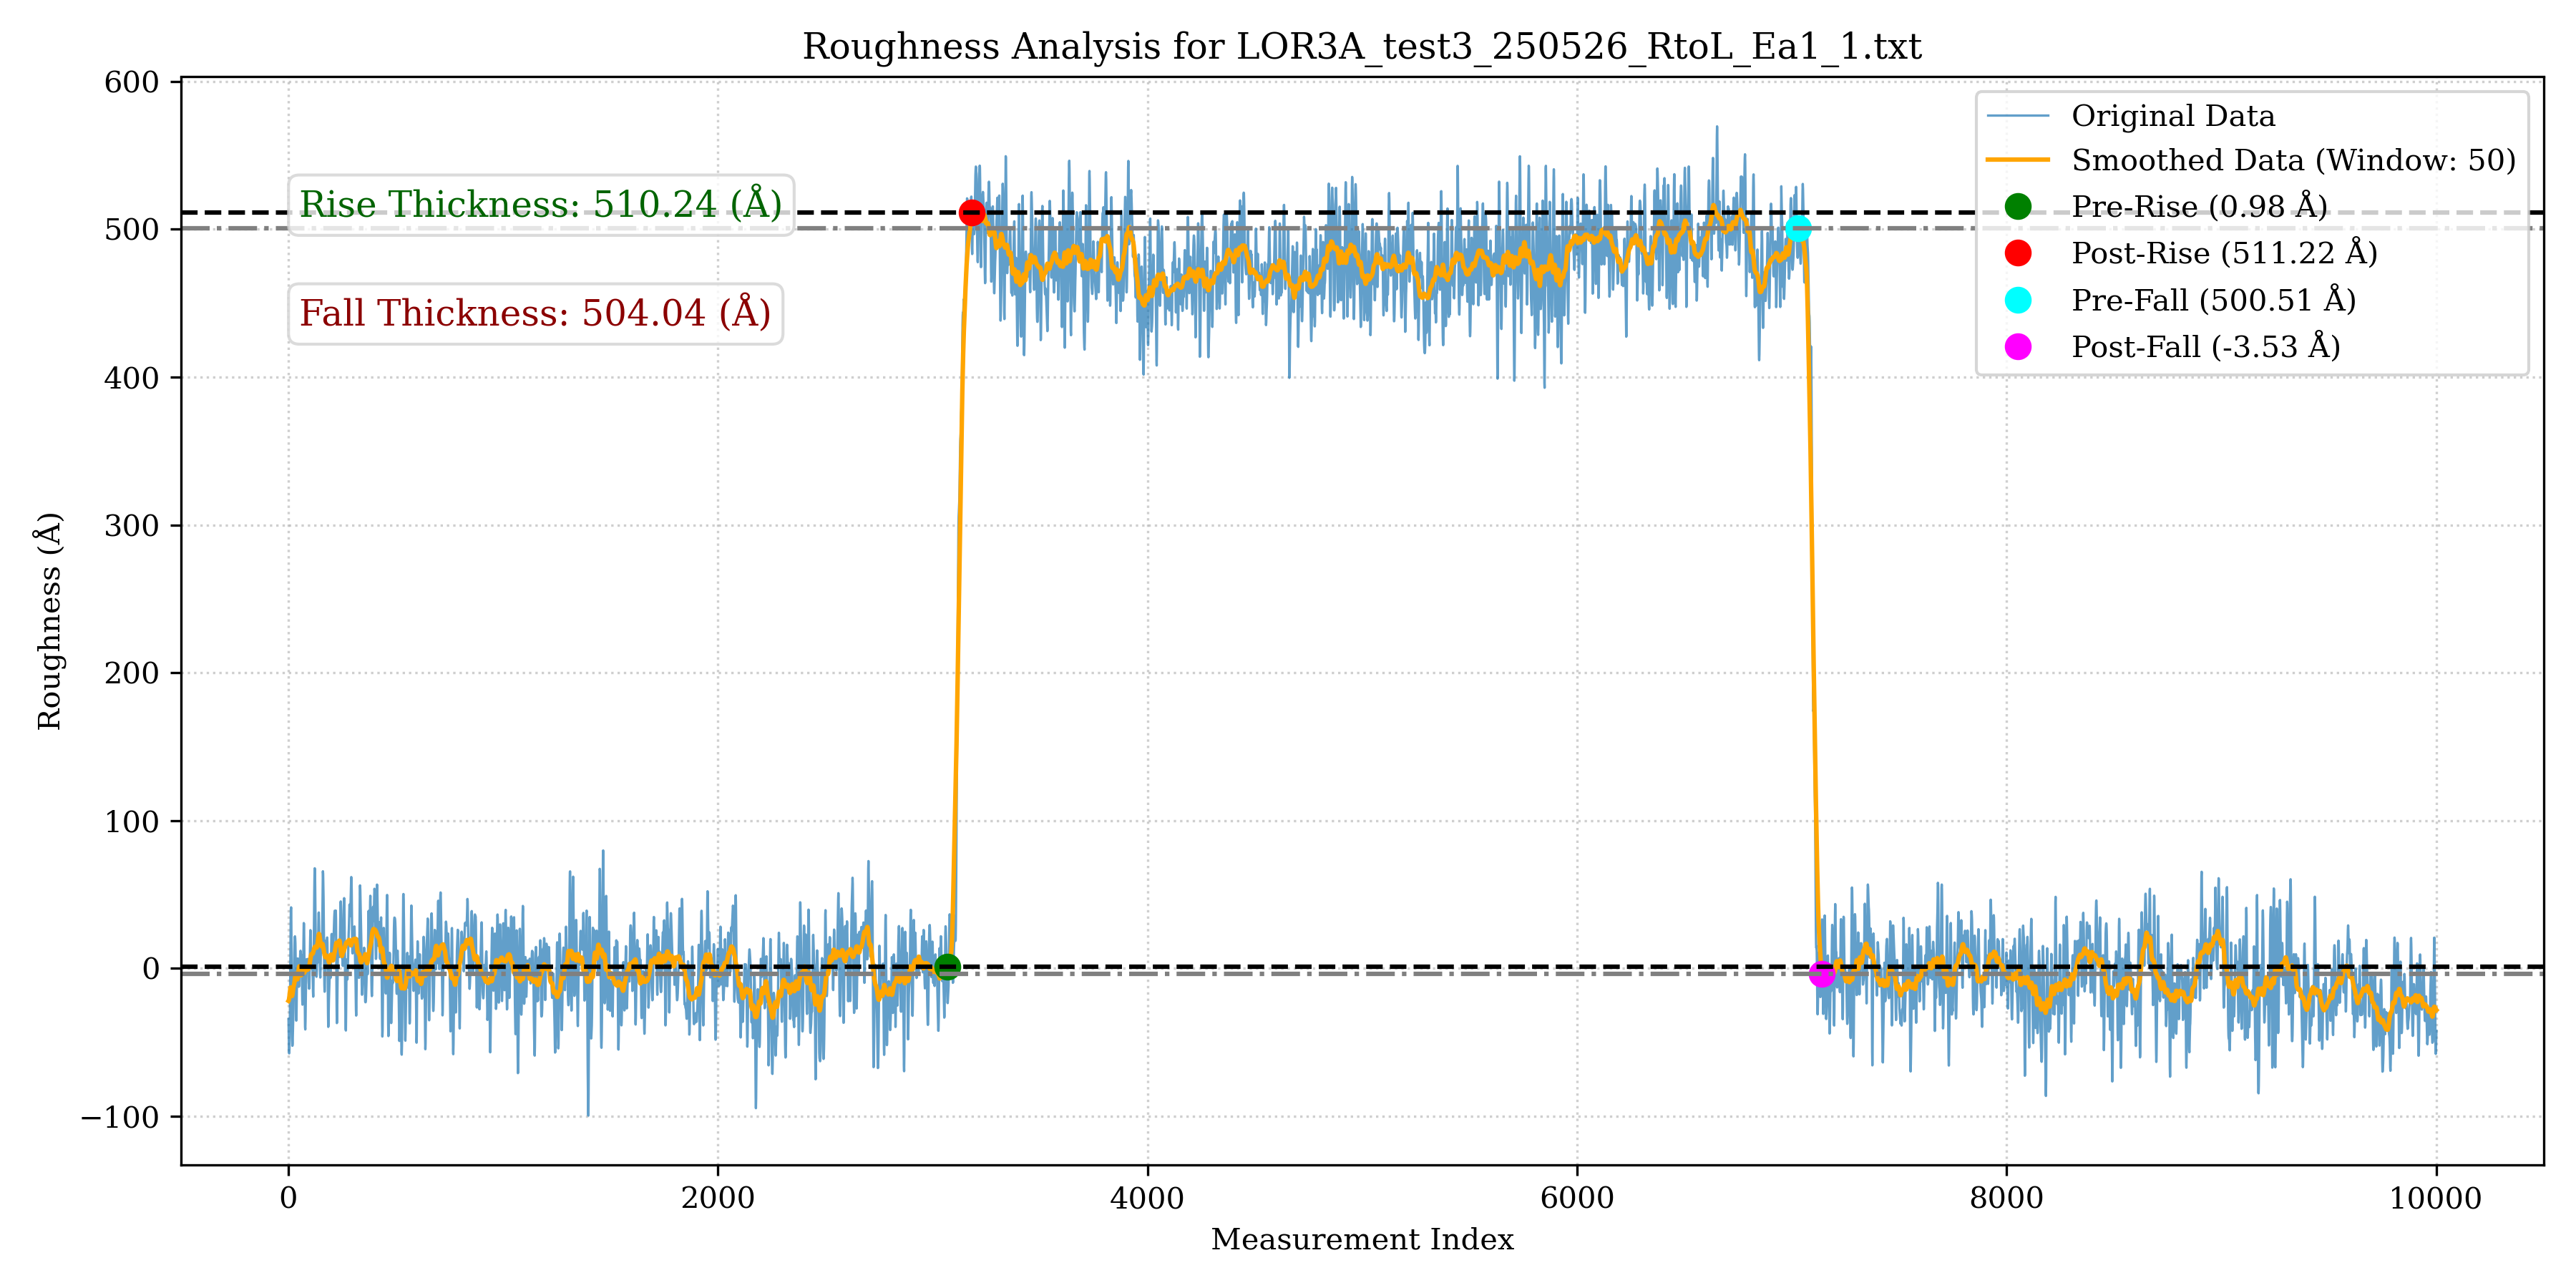
\includegraphics[width=\textwidth]{LOR3A_test3_250526_RtoL_Ea1_1.png}
    \label{fig:LOR3Atest3250526RtoLEa11}
\end{figure}
\begin{figure}[H]
    \centering
    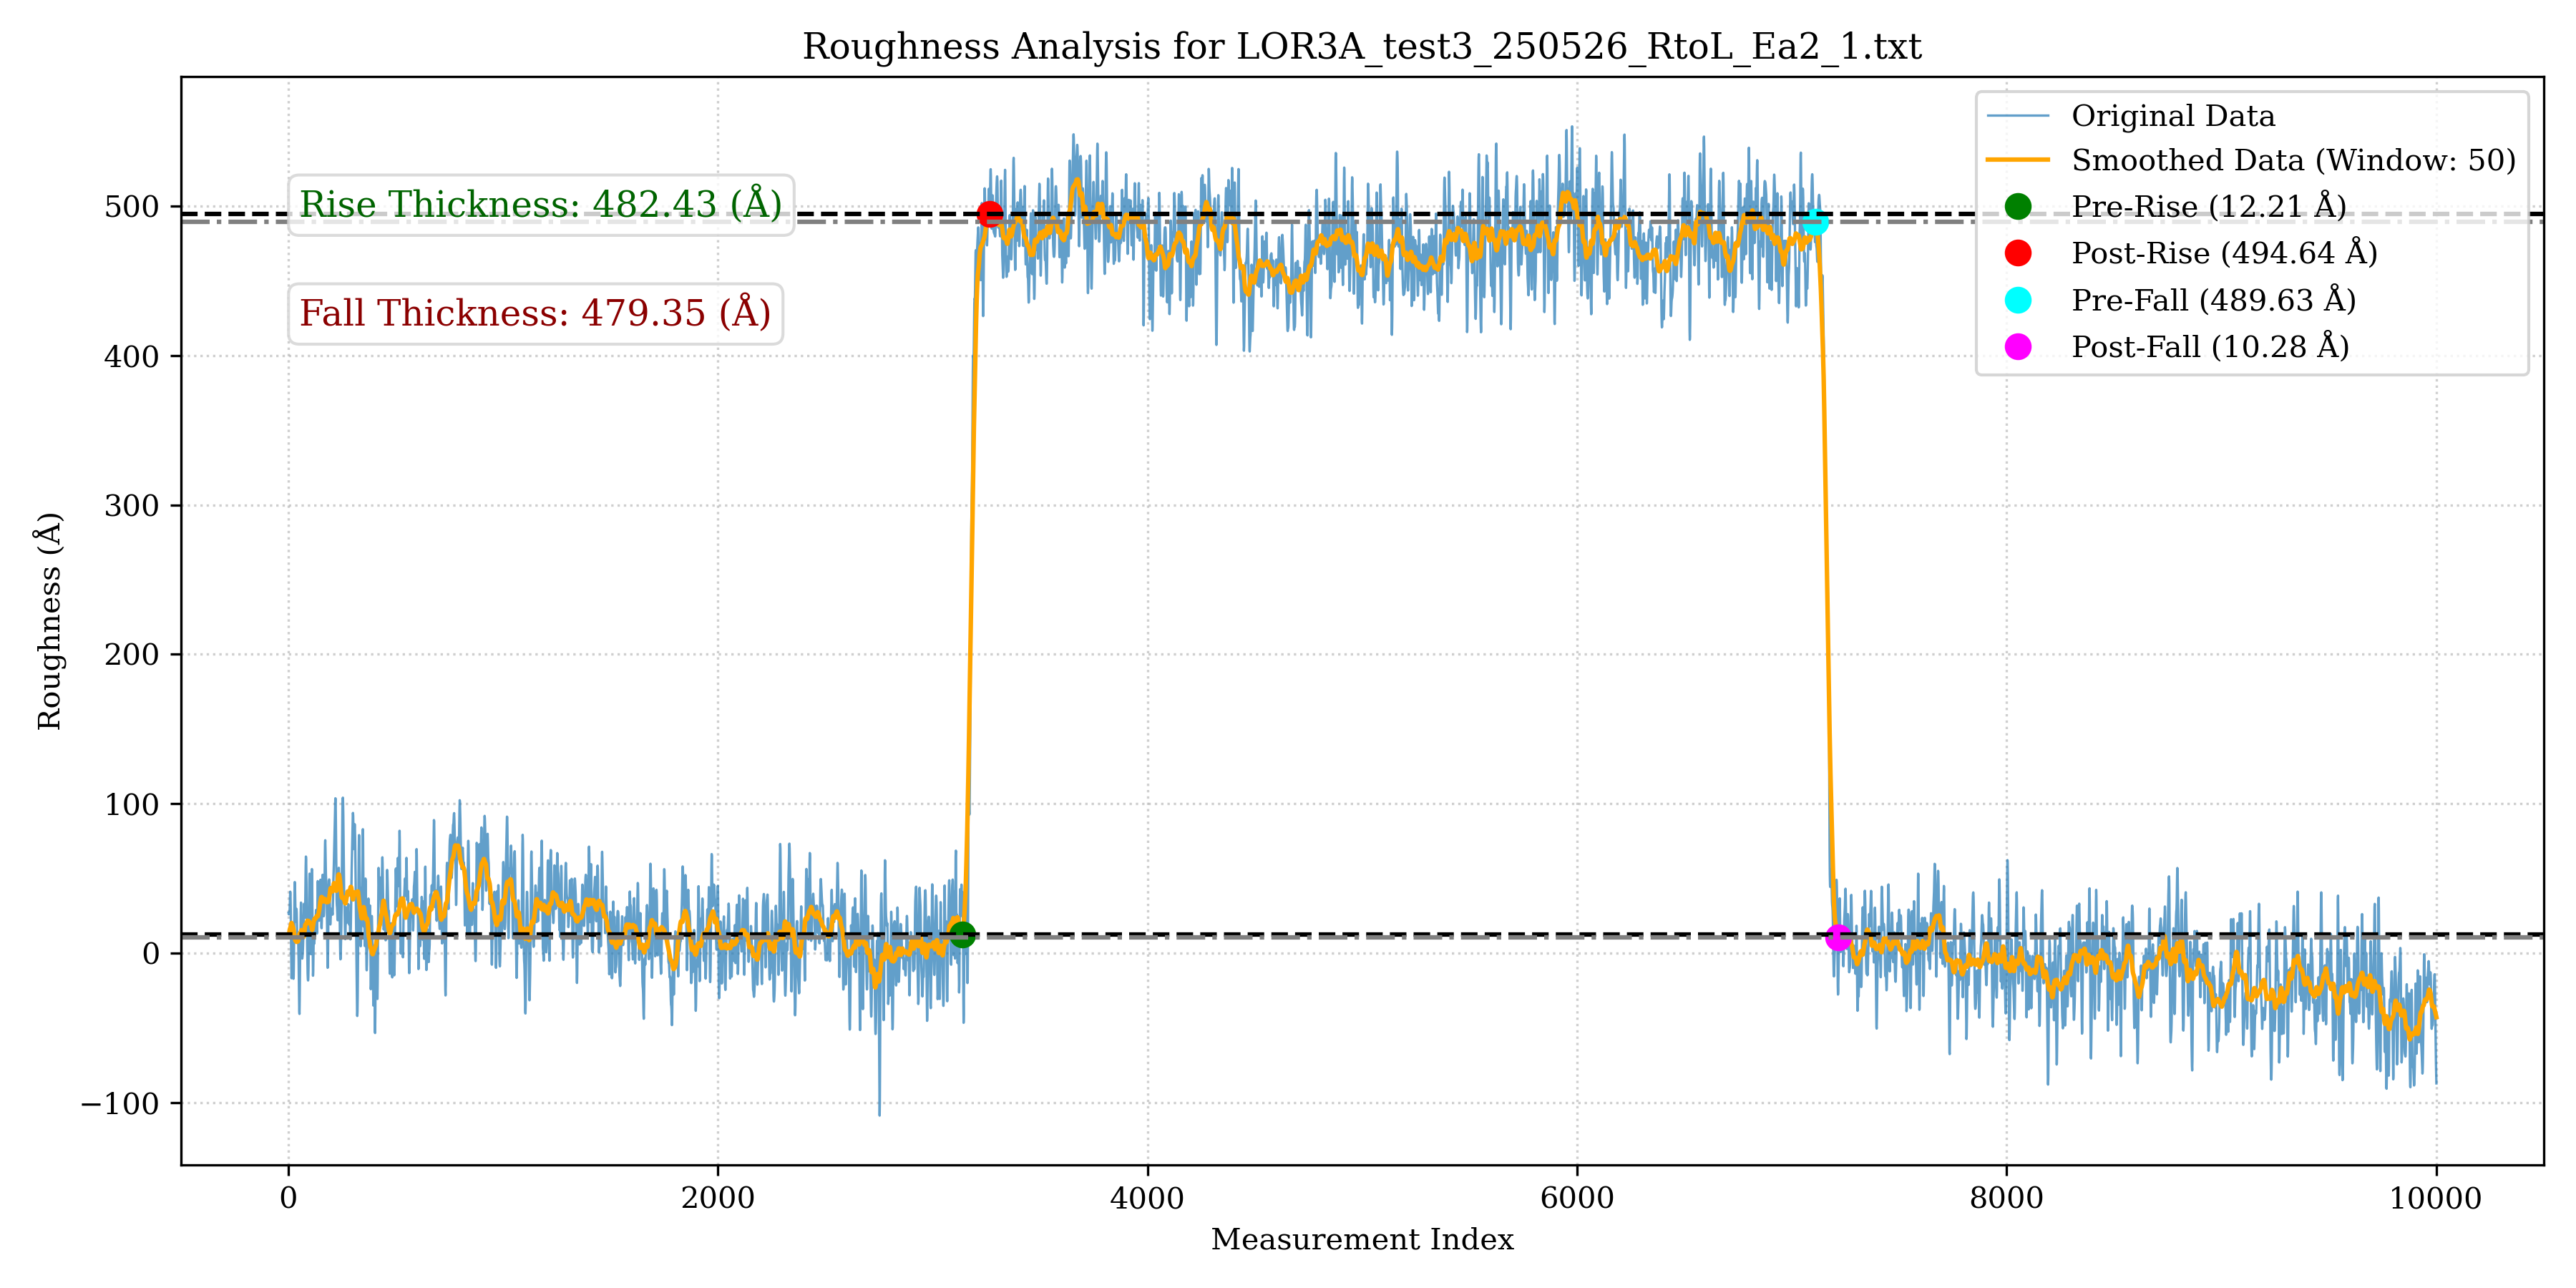
\includegraphics[width=\textwidth]{LOR3A_test3_250526_RtoL_Ea2_1.png}
    \label{fig:LOR3Atest3250526RtoLEa21}
\end{figure}
\begin{figure}[H]
    \centering
    \includegraphics[width=\textwidth]{LOR3A_test3_250526_RtoL_Ea3_1.png}
    \label{fig:LOR3Atest3250526RtoLEa31}
\end{figure}
\begin{figure}[H]
    \centering
    \includegraphics[width=\textwidth]{LOR3A_test3_250526_RtoL_Ea3_2.png}
    \label{fig:LOR3Atest3250526RtoLEa32}
\end{figure}
\begin{figure}[H]
    \centering
    \includegraphics[width=\textwidth]{LOR3A_test3_250526_RtoL_Ea4_1.png}
    \label{fig:LOR3Atest3250526RtoLEa41}
\end{figure}
\begin{figure}[H]
    \centering
    \includegraphics[width=\textwidth]{LOR3A_test3_250526_RtoL_Ea5_1.png}
    \label{fig:LOR3Atest3250526RtoLEa51}
\end{figure}

\end{document}
